\documentclass[12pt,a4paper]{report}

% =========================================================================
% GÓI THƯ VIỆN & CẤU HÌNH CƠ BẢN (XELATEX COMPATIBLE)
% =========================================================================
\usepackage{fontspec}
\setmainfont{Times New Roman}

\usepackage[top=2.5cm, bottom=2.5cm, left=3.0cm, right=2.0cm]{geometry}
\usepackage{amsmath, amsfonts, amssymb}
\usepackage{graphicx}
\usepackage{booktabs}
\usepackage{tabularx}
\usepackage{multirow}
\usepackage{array}
\usepackage{float}
\usepackage{xcolor}
\usepackage{colortbl}
\usepackage{tikz}
\usetikzlibrary{calc, shapes.geometric, arrows.meta, positioning}
\usepackage{hyperref}
\usepackage{fancyhdr}
\usepackage{titlesec}
\usepackage{caption}
\usepackage{subcaption}
\usepackage{enumitem}
\usepackage{listings}
\usepackage{tcolorbox}

% Cấu hình Hyperref
\hypersetup{
    colorlinks=true,
    linkcolor=blue!80!black,
    citecolor=green!60!black,
    urlcolor=blue!70!black,
    pdftitle={Báo Cáo Assignment 05 - Phát Triển Hệ Thống Thông Minh},
    pdfauthor={Phạm Văn Tư - B23DCCN879}
}

% Cấu hình Code Listing cho Python / PyTorch
\definecolor{codegreen}{rgb}{0,0.6,0}
\definecolor{codegray}{rgb}{0.5,0.5,0.5}
\definecolor{codepurple}{rgb}{0.58,0,0.82}
\definecolor{backcolour}{rgb}{0.96,0.97,0.98}

\lstdefinestyle{mystyle}{
    backgroundcolor=\color{backcolour},   
    commentstyle=\color{codegreen},
    keywordstyle=\color{blue!80!black}\bfseries,
    numberstyle=\tiny\color{codegray},
    stringstyle=\color{codepurple},
    basicstyle=\ttfamily\footnotesize,
    breakatwhitespace=false,         
    breaklines=true,                 
    captionpos=b,                    
    keepspaces=true,                 
    numbers=left,                    
    numbersep=5pt,                  
    showspaces=false,                
    showstringspaces=false,
    showtabs=false,                  
    tabsize=2,
    frame=single,
    rulecolor=\color{black!20}
}
\lstset{style=mystyle}

% Định dạng tiêu đề chương, mục chuẩn học thuật PTIT
\titleformat{\chapter}[display]
  {\normalfont\bfseries\color{blue!80!black}}
  {\filleft\Large\bfseries\chaptertitlename\ \thechapter}
  {1ex}
  {\titlerule\vspace{1ex}\filright\LARGE}
  [\vspace{1ex}\titlerule]

\titleformat{\section}
  {\normalfont\Large\bfseries\color{blue!70!black}}
  {\thesection}{1em}{}

\titleformat{\subsection}
  {\normalfont\large\bfseries\color{black!85}}
  {\thesubsection}{1em}{}

% Header & Footer
\pagestyle{fancy}
\fancyhf{}
\fancyhead[R]{\small\itshape Báo cáo Assignment 05: Chuyên đề Mạng Nơ-ron Tích chập (CNN)}
\fancyfoot[C]{\thepage}
\renewcommand{\headrulewidth}{0.4pt}
\renewcommand{\footrulewidth}{0.4pt}
\setlength{\headheight}{14pt}

% =========================================================================
% BẮT ĐẦU TÀI LIỆU
% =========================================================================
\begin{document}

% -------------------------------------------------------------------------
% TRANG BÌA CHUẨN PTIT (ĐỒNG BỘ 100% VỚI TEMPLATE CÁC ASSIGNMENT TRƯỚC)
% -------------------------------------------------------------------------
\begin{titlepage}
\begin{tikzpicture}[remember picture, overlay]
    \node[anchor=center] at (current page.center) {
        
\includegraphics[width=\dimexpr\paperwidth-2.0cm\relax, height=\dimexpr\paperheight-2.0cm\relax]{images/ptit_cover_border.jpeg}
    };
\end{tikzpicture}

\begin{center}
    \vspace*{-0.2cm}
    {\fontsize{14.5pt}{19pt}\selectfont \textbf{HỌC VIỆN CÔNG NGHỆ BƯU CHÍNH VIỄN THÔNG}}\\[0.3cm]
    {\fontsize{14.5pt}{19pt}\selectfont \textbf{KHOA CÔNG NGHỆ THÔNG TIN 1}}\\[0.3cm]
    {\fontsize{14.5pt}{19pt}\selectfont \textbf{HỌC PHẦN PHÁT TRIỂN CÁC HỆ THỐNG THÔNG MINH}}\\[1.1cm]
    
    % Logo PTIT
    
\includegraphics[width=4.5cm]{images/ptit_logo.png}\\[1.3cm]
    
    {\fontsize{18pt}{22pt}\selectfont \textbf{ASSIGNMENT 05}}\\[0.4cm]
    {\fontsize{15pt}{20pt}\selectfont \textbf{MẠNG NƠ-RON TÍCH CHẬP CNN}}\\[1.2cm]
\end{center}

\begin{flushleft}
    \hspace{2.8cm}
    \begin{tabular}{ll}
        \textbf{Lớp:} & D23CTPM01 \\[0.3cm]
        \textbf{Họ và tên:} & Phạm Văn Tư \\[0.3cm]
        \textbf{Mã sinh viên:} & B23DCCN879 \\[0.3cm]
        \textbf{Giảng viên hướng dẫn:} & PGS.TS Trần Đình Quế \\[0.3cm]
        \textbf{Học kỳ:} & Học kỳ 1 năm học 2026 – 2027
    \end{tabular}
\end{flushleft}

\vfill
\begin{center}
    {\fontsize{12pt}{15pt}\selectfont \textbf{Hà Nội, 2026}}\\[0.4cm]
\end{center}
\end{titlepage}

% -------------------------------------------------------------------------
% MỤC LỤC & DANH MỤC HÌNH ẢNH / BẢNG BIỂU
% -------------------------------------------------------------------------
\pagenumbering{roman}
\tableofcontents
\newpage
\listoffigures
\listoftables
\newpage
\pagenumbering{arabic}

% =========================================================================
% TỔNG QUAN BÁO CÁO
% =========================================================================
\chapter*{Tổng Quan Báo Cáo}
\addcontentsline{toc}{chapter}{Tổng Quan Báo Cáo}

Trong kỹ nghệ phát triển các hệ thống thông minh xử lý dữ liệu không gian đa chiều (Thị giác máy tính và Tín hiệu y sinh), \textbf{Mạng Nơ-ron Tích chập (Convolutional Neural Networks -- CNN)} đóng vai trò là một trong những bước nhảy vọt quan trọng nhất của học sâu hiện đại. Khác với cách tiếp cận ``hộp đen'', việc làm chủ CNN đòi hỏi một phương pháp luận toán học chặt chẽ: giải phẫu mạng nơ-ron thành chuỗi các ánh xạ và biểu diễn toàn bộ kiến trúc dưới dạng một \textbf{hàm hợp toán học (Composite Function)}.

Nội dung nghiên cứu và thực nghiệm của báo cáo tập trung vào các trọng tâm khoa học cốt lõi:
\begin{enumerate}[leftmargin=2em]
    \item \textbf{Chương 1 -- Nền tảng Toán học \& Mô hình Hàm hợp:} Trình bày cơ sở giải tích của các toán tử thành phần (Tích chập 2D đa kênh, Hàm kích hoạt phi tuyến, Gom cụm Max Pooling, Gom cụm toàn cục GAP) và mô hình hóa cấu trúc mạng nơ-ron tích chập dưới dạng một hàm hợp toán học liên tục kèm hiện thực hóa thuật toán.
    \item \textbf{Chương 2 -- Các Mô hình Tiến hóa Kiến trúc:} Khảo sát và hiện thực hóa 3 hướng phát triển kinh điển của CNN: Khối VGG (Thừa số hóa bộ lọc $3\times 3$), Khối ResNet (Học phần dư và giải quyết suy biến gradient qua kết nối tắt), và Khối MobileNet (Tích chập tách rời theo chiều sâu Depthwise Separable Convolution).
    \item \textbf{Chương 3 -- Kỹ Thuật Tối Ưu Huấn Luyện, Điều Chuẩn, Chuyển Giao Tri Thức \& Đối Chuẩn Thực Nghiệm:} Phân tích toán học các giải pháp vượt qua thách thức mạng sâu (Z-score, Batch Normalization, Skip Connection), bộ 5 kỹ thuật điều chuẩn chống quá khớp (Ablation Study trên CIFAR-10), phương pháp luận Transfer Learning (Network Surgery) và đối chuẩn thực chiến đa kiến trúc kèm phân tích đường biên Pareto và không gian ẩn PCA.
    \item \textbf{Chương 4 -- Khảo Sát Thực Nghiệm, Khám Phá Dữ Liệu (EDA) \& Tiền Xử Lý 3 Bộ Dữ Liệu Đa Miền:} Kiểm toán dị thường y sinh trên dữ liệu bảng (Pima Diabetes), giải mã đặc trưng quang học ảnh ngoại cảnh (SVHN) và hình thái tế bào học hiển vi (BloodMNIST), thiết lập ma trận đối chuẩn và đóng gói các luồng nạp dữ liệu PyTorch tối ưu.
    \item \textbf{Chương 5 -- Hiện Thực Hóa, Huấn Luyện \& Đối Chuẩn Thực Nghiệm 4 Kiến Trúc CNN:} Huấn luyện, đo kiểm và đối chuẩn đa chiều 4 mô hình học sâu (Baseline CNN, VGG-11, ResNet-18, MobileNetV2) trên các tập dữ liệu đã chuẩn hóa.
\end{enumerate}

\begin{tcolorbox}[colback=blue!3!white, colframe=blue!75!black, title=\textbf{Kho lưu trữ Mã nguồn Thực nghiệm}]
\small\raggedright
\begin{itemize}[leftmargin=1.5em, itemsep=4pt]
    \item \textbf{Kho lưu trữ dự án chính thức:}\\
    \href{https://github.com/phamtu2x5/INTELLIGENT-SYSTEM-DEVELOPMENT}{\texttt{INTELLIGENT-SYSTEM-DEVELOPMENT}}
    \item \textbf{Mã nguồn Thực nghiệm Nền tảng Toán học \& Hàm Hợp CNN:}\\
    \href{https://github.com/phamtu2x5/INTELLIGENT-SYSTEM-DEVELOPMENT/tree/main/src/Assigment\%2005}{\texttt{Mã nguồn thực nghiệm trực tuyến (GitHub)}}
\end{itemize}
\end{tcolorbox}

\newpage

% =========================================================================
% CHƯƠNG 1: CƠ SỞ LÝ THUYẾT VỀ MẠNG NƠ-RON TÍCH CHẬP & BIỂU DIỄN HÀM HỢP
% =========================================================================
\chapter{Cơ Sở Lý Thuyết Về Mạng Nơ-ron Tích Chập \& Biểu Diễn Hàm Hợp}

\section{Cảm Hứng Sinh Học \& Động Lực Chuyển Đổi Từ MLP Sang CNN}

\subsection{Cảm Hứng Sinh Học Từ Vỏ Não Thị Giác (Visual Cortex)}
Mạng Nơ-ron Tích chập (Convolutional Neural Networks -- CNN) không đơn thuần là một mô hình toán học trừu tượng, mà được truyền cảm hứng sâu sắc từ các khám phá kinh điển về hệ thống thị giác sinh học. Năm 1959, hai nhà sinh lý học David Hubel và Torsten Wiesel (được trao giải Nobel Y học năm 1981) đã thực hiện các thí nghiệm đo điện thế hoạt động của các tế bào nơ-ron tại vỏ não thị giác sơ cấp (Primary Visual Cortex -- V1) của loài mèo và linh trưởng khi tiếp nhận các kích thích ánh sáng:
\begin{itemize}[leftmargin=2em]
    \item \textbf{Tế bào Đơn giản (Simple Cells):} Chỉ phản ứng mạnh khi có các kích thích dạng đường thẳng hoặc cạnh biên có phương hướng góc cụ thể (ví dụ: vạch sáng nằm ngang hoặc nghiêng $45^\circ$) xuất hiện trong một vùng thụ cảm không gian rất hẹp.
    \item \textbf{Tế bào Phức tạp (Complex Cells):} Nhận tín hiệu tổng hợp từ nhiều tế bào đơn giản liền kề, phản ứng với các cạnh có hướng nhất định nhưng cho phép cạnh đó chuyển dịch một khoảng nhỏ trong không gian (đặt nền móng cho tính bất biến cục bộ).
    \item \textbf{Cơ chế Xếp tầng Thứ bậc (Hierarchical Processing):} Vỏ não thị giác xử lý thông tin quang học theo chuỗi thứ bậc từ thấp lên cao: từ việc nhận diện các điểm sáng rời rạc $\to$ phát hiện các đường biên, góc cạnh $\to$ tổng hợp thành các đường cong, họa tiết cục bộ $\to$ nhận diện các bộ phận $\to$ định danh toàn bộ cấu trúc vật thể hoàn chỉnh.
\end{itemize}
Kiến trúc CNN hiện đại kế thừa hoàn hảo nguyên lý này: các tầng tích chập ban đầu trích xuất các đặc trưng hình học tần số cao (cạnh, góc), trong khi các tầng tích chập sâu hơn trích xuất các đặc trưng ngữ nghĩa trừu tượng có tính khái quát cao.

\newpage

\subsection{Không Gian Biểu Diễn Ảnh Số: Ma Trận 2D \& Tensor 3D}
Trong xử lý tín hiệu số, một bức ảnh số là kết quả của việc rời rạc hóa cường độ ánh sáng trên một lưới tọa độ không gian hai chiều:
\begin{itemize}[leftmargin=2em]
    \item \textbf{Ảnh đơn sắc (Grayscale):} Được mô hình hóa bởi ma trận hai chiều $\mathbf{X} \in \mathbb{R}^{H \times W}$, trong đó mỗi phần tử $x_{i, j} \in [0, 255]$ là một giá trị độ sáng vô hướng tại tọa độ hàng $i$ và cột $j$ ($H$ là chiều cao, $W$ là chiều rộng). Mức $0$ tương ứng với độ tối tuyệt đối (mức đen) và mức $255$ đại diện cho cường độ sáng tối đa (mức trắng).
    \item \textbf{Ảnh màu tự nhiên (RGB):} Được mô hình hóa bởi một Tensor ba chiều $\mathbf{X} \in \mathbb{R}^{H \times W \times C}$ với $C = 3$ kênh màu cơ bản (Red, Green, Blue). Mỗi điểm ảnh tại vị trí $(i, j)$ được định nghĩa bởi một vector 3 chiều $[R, G, B]^T$, phản ánh cường độ phổ ánh sáng tại tọa độ đó (Hình \ref{fig:image_matrix_and_tensor}).
\end{itemize}

\begin{figure}[H]
\centering
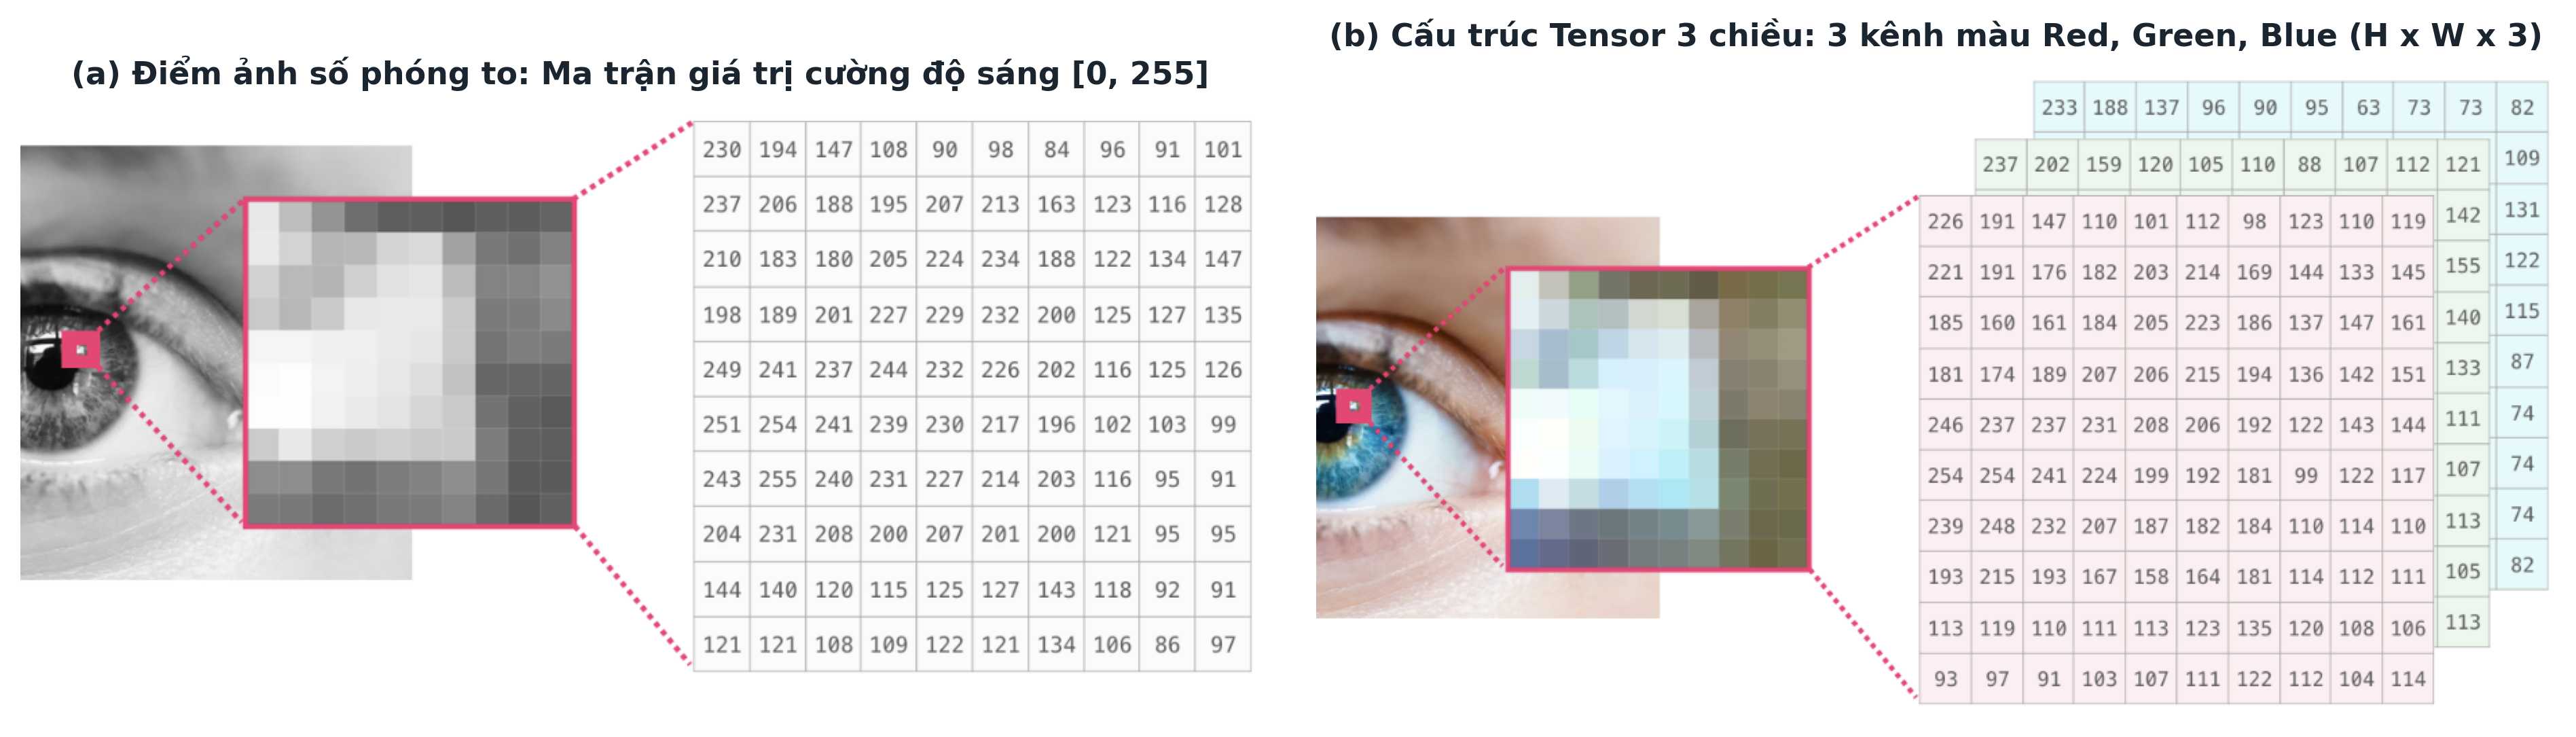
\includegraphics[width=0.95\textwidth]{images/theory_image_pixel_matrix_and_rgb_tensor.png}
\caption{Biểu diễn ảnh số: (a) Ảnh đơn sắc 2D và (b) Ảnh màu RGB 3D}
\label{fig:image_matrix_and_tensor}
\end{figure}

\newpage

\subsection{Hạn Chế Cố Hữu Của Mạng Nơ-ron Truyền Thẳng (MLP) Khi Xử Lý Ảnh}
Trước khi mạng tích chập trở thành tiêu chuẩn, phương pháp tiếp cận phổ biến là sử dụng mạng nơ-ron truyền thẳng đa tầng (Multi-Layer Perceptron -- MLP). Để đưa một bức ảnh hai hoặc ba chiều vào MLP, bước bắt buộc đầu tiên là thực hiện phép làm phẳng (Flatten):
\begin{equation}
\text{vec}: \mathbb{R}^{H \times W \times C} \longrightarrow \mathbb{R}^{D}, \quad D = H \cdot W \cdot C
\end{equation}

\begin{figure}[H]
\centering
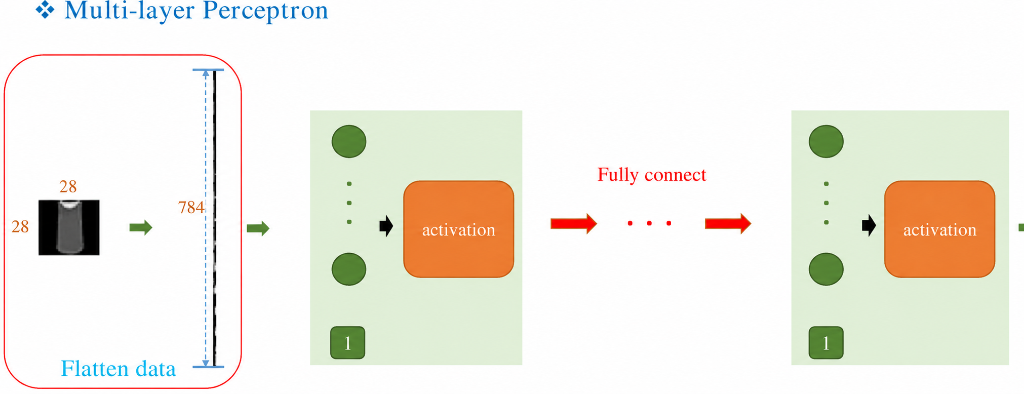
\includegraphics[width=0.88\textwidth]{images/slide15_mlp_flatten.png}
\caption{Cơ chế làm phẳng (Flatten) vector hóa ảnh trong mạng MLP}
\label{fig:mlp_flatten}
\end{figure}

Thao tác này làm phát sinh ba nhược điểm nghiêm trọng trong thị giác máy tính:
\begin{enumerate}[leftmargin=1.5em]
    \item \textbf{Phá hủy hoàn toàn cấu trúc không gian (Spatial Topology Destruction):} Phép làm phẳng coi mọi điểm ảnh là độc lập. Mối tương quan cục bộ tự nhiên giữa hai điểm ảnh nằm sát nhau theo trục dọc $(i, j)$ và $(i+1, j)$ bị kéo dãn cách nhau hàng trăm hoặc hàng ngàn chỉ số trong vector phẳng, triệt tiêu hoàn toàn thông tin về hình dạng, biên giới hình học và tính liên tục quang học.
    \item \textbf{Bùng nổ số lượng tham số (Parameter Explosion):} Trong tầng liên kết đầy đủ (Fully Connected / Dense Layer), mỗi nơ-ron phải kết nối tới toàn bộ $D$ điểm ảnh. Xét một bức ảnh kích thước nhỏ $64 \times 64 \times 3 \approx 12,288$ phần tử. Nếu nối tới một tầng ẩn gồm $1,024$ nơ-ron, ma trận trọng số cần tới $12,288 \times 1,024 \approx 12.58$ triệu tham số. Khối lượng tham số khổng lồ này gây ra hiện tượng quá khớp (Overfitting) nặng nề và đòi hỏi chi phí tính toán cực lớn.
    \item \textbf{Nhạy cảm và thiếu tính bất biến với dịch chuyển (Lack of Translation Invariance):} Nếu một vật thể (chữ số, khuôn mặt, chiếc lá) bị dịch chuyển lệch sang một góc khác của ảnh, mạng MLP hoàn toàn không thể nhận biết được vì bộ trọng số tương ứng ở tọa độ mới chưa từng được huấn luyện với mẫu đặc trưng đó.
\end{enumerate}

\subsection{Hai Nguyên Lý Kiến Trúc Đột Phá Của CNN}
Nhằm giải quyết triệt để ba rào cản trên của MLP, kiến trúc CNN tích hợp hai nguyên lý nền tảng:
\begin{itemize}[leftmargin=2em]
    \item \textbf{Liên kết cục bộ (Local Connectivity / Receptive Field):} Thay vì kết nối toàn phần tới mọi điểm ảnh, mỗi nơ-ron trong tầng tích chập chỉ kết nối với một vùng lân cận không gian nhỏ (Local Receptive Field) kích thước $K_H \times K_W$ thông qua một cửa sổ trượt. Điều này phù hợp với định luật vật lý tự nhiên: các điểm ảnh gần nhau có mối tương quan mạnh mẽ hơn các điểm ảnh ở xa.
    \item \textbf{Chia sẻ trọng số (Weight Sharing):} Cùng một bộ lọc trọng số (Kernel) kích thước cố định được quét tuần tự trên toàn bộ ảnh. Nếu một mẫu đặc trưng (ví dụ: góc nghiêng hoặc cạnh dọc) có ý nghĩa nhận dạng ở góc trái ảnh, thì cùng bộ lọc đó cũng có thể phát hiện mẫu tương tự ở góc phải ảnh. Nguyên lý này giúp giảm số lượng tham số tự do từ hàng triệu xuống chỉ còn vài trăm hoặc vài ngàn tham số.
\end{itemize}

\begin{figure}[H]
\centering
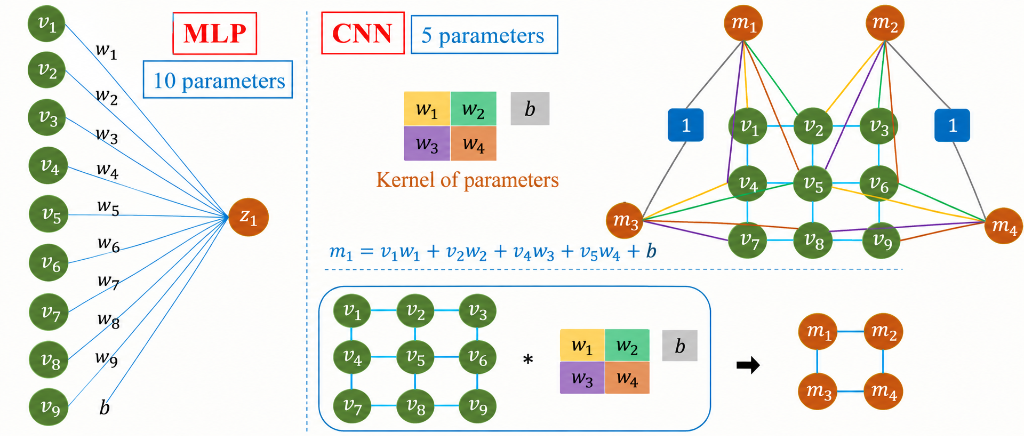
\includegraphics[width=0.88\textwidth]{images/slide16_mlp_vs_cnn_params.png}
\caption{So sánh cơ chế kết nối và tham số giữa MLP và CNN}
\label{fig:mlp_vs_cnn_params}
\end{figure}

\newpage

\section{Bản Chất Toán Học \& Tính Toán Từng Bước Của Phép Tích Chập 2D}

\subsection{Bản Chất Toán Học Của Cửa Sổ Trượt Tích Chập}
Trong học máy, toán tử tích chập (thực chất là phép tương quan chéo rời rạc -- Cross-Correlation) là một ánh xạ trượt một ma trận trọng số nhỏ gọi là \textbf{Bộ lọc (Filter / Kernel)} trên toàn bộ bề mặt của ảnh đầu vào. Tại mỗi vị trí dừng, kernel thực hiện phép tính tích vô hướng Frobenius (nhân từng phần tử tương ứng rồi cộng tổng) giữa các trọng số và vùng ảnh cục bộ:

\begin{figure}[H]
\centering
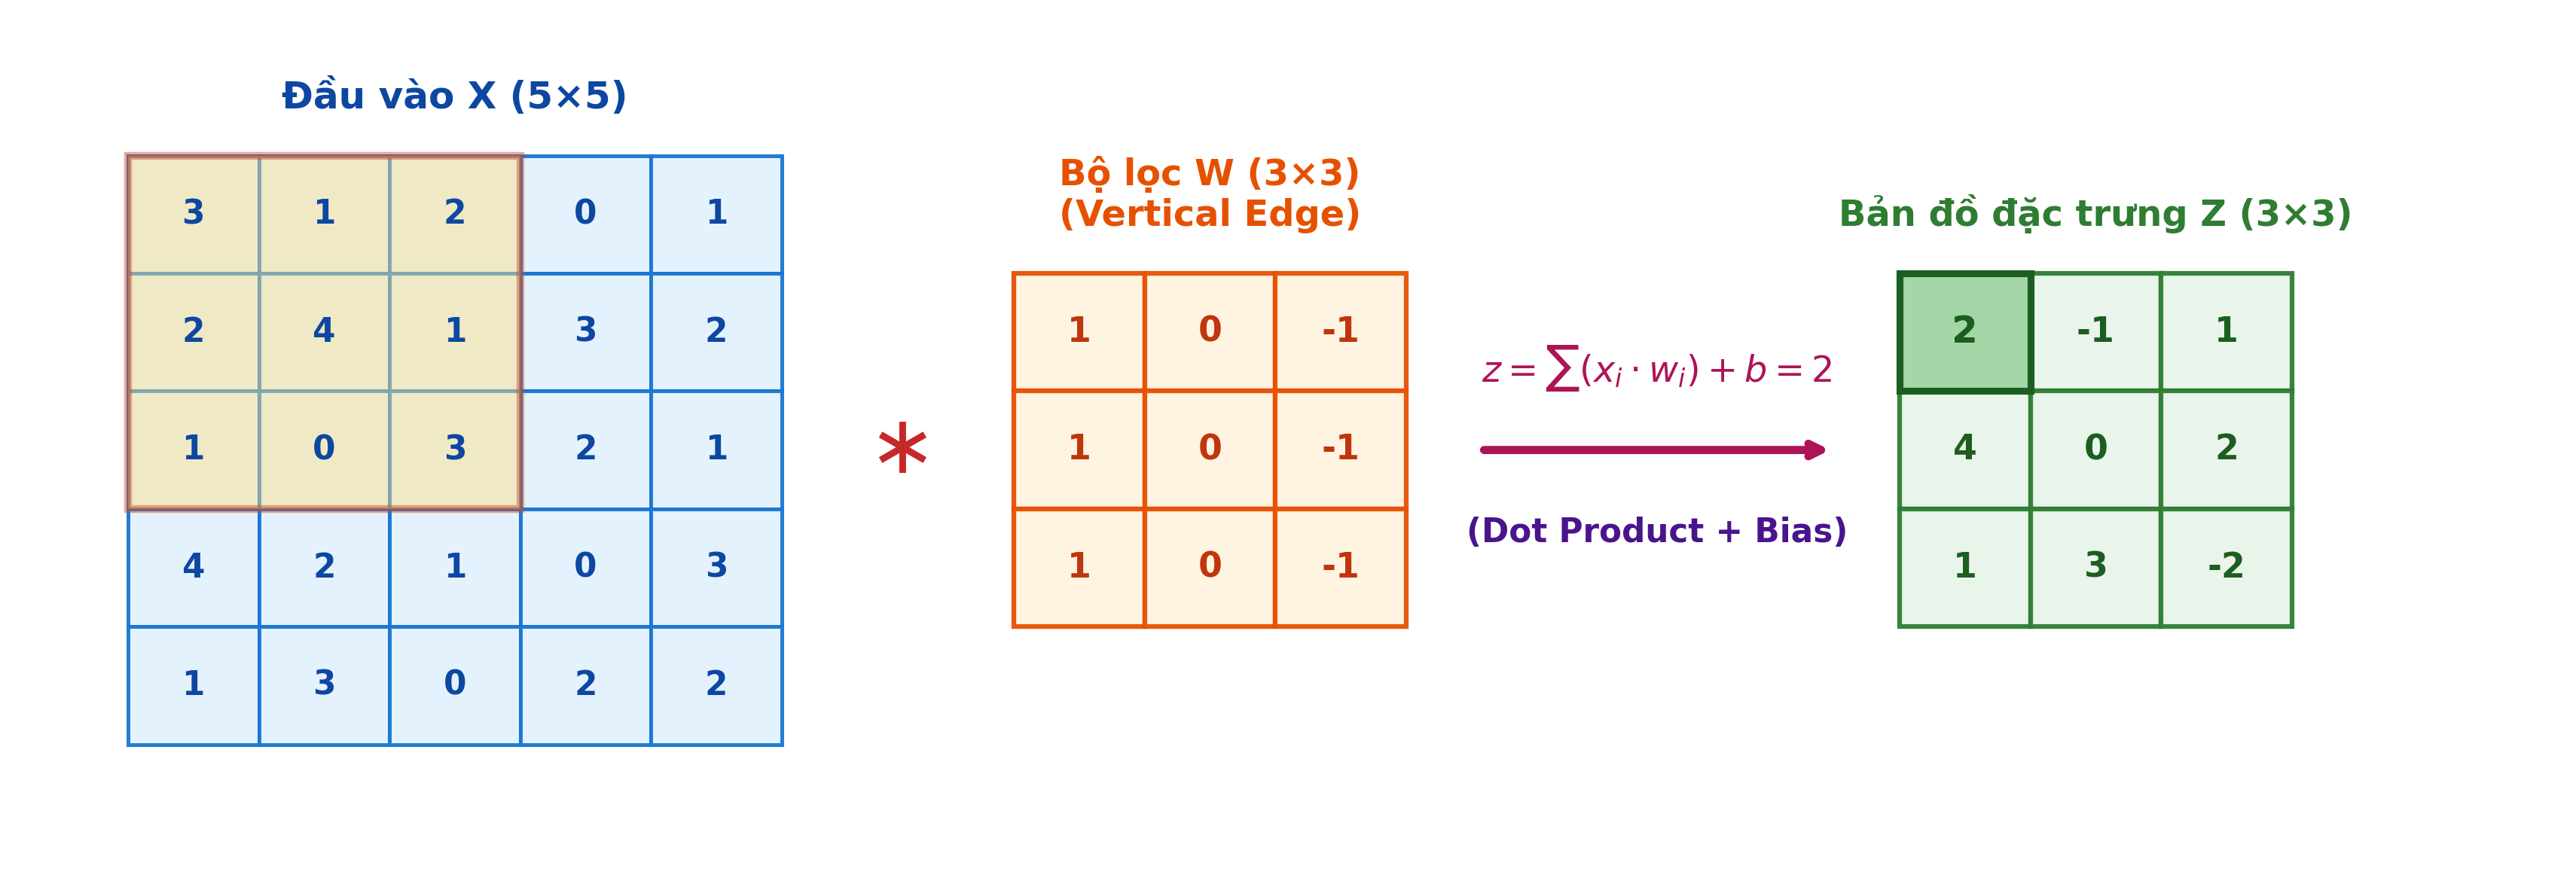
\includegraphics[width=0.92\textwidth]{images/theory_convolution_operation.png}
\caption{Nguyên lý tích chập 2D qua cửa sổ trượt cục bộ}
\label{fig:conv_operation}
\end{figure}

\newpage

\subsection{Minh Họa Tính Toán Số Học Từng Bước (Step-by-Step Convolution)}
Để hiểu trực quan và tường minh nhất quy trình tính toán, xét một ma trận ảnh đơn kênh đầu vào kích thước $5 \times 5$, một kernel trọng số kích thước $3 \times 3$ và hệ số độ chệch $b = 1$:
\begin{equation}
\mathbf{X} = \begin{bmatrix} 1 & 2 & 0 & 1 & 0 \\ 0 & 1 & 1 & 2 & 1 \\ 2 & 1 & 0 & 0 & 3 \\ 1 & 0 & 2 & 1 & 1 \\ 0 & 3 & 1 & 2 & 0 \end{bmatrix}, \quad
\mathbf{W} = \begin{bmatrix} 1 & 0 & -1 \\ 1 & 0 & -1 \\ 1 & 0 & -1 \end{bmatrix}, \quad b = 1
\end{equation}

\noindent \textbf{Bước 1: Tính toán tại vị trí ban đầu (0, 0):} \\
Khi kernel đặt tại vị trí góc trên bên trái của ảnh, cửa sổ trượt bao phủ vùng tiếp nhận cục bộ $\mathbf{X}_{\text{patch}}^{(0, 0)}$ kích thước $3 \times 3$. Giá trị kích hoạt thô đầu ra $Z(0, 0)$ được tính bằng tích vô hướng Frobenius từng phần tử cộng dồn với bias:
\begin{align}
Z(0, 0) &= \sum_{p=0}^2 \sum_{q=0}^2 X_{\text{patch}}(p, q) \cdot W(p, q) + b \nonumber\\
&= (1 \cdot 1 + 2 \cdot 0 + 0 \cdot (-1)) + (0 \cdot 1 + 1 \cdot 0 + 1 \cdot (-1)) + (2 \cdot 1 + 1 \cdot 0 + 0 \cdot (-1)) + 1 \nonumber\\
&= (1 + 0 + 0) + (0 + 0 - 1) + (2 + 0 + 0) + 1 = 1 - 1 + 2 + 1 = 3
\end{align}

\begin{figure}[H]
\centering
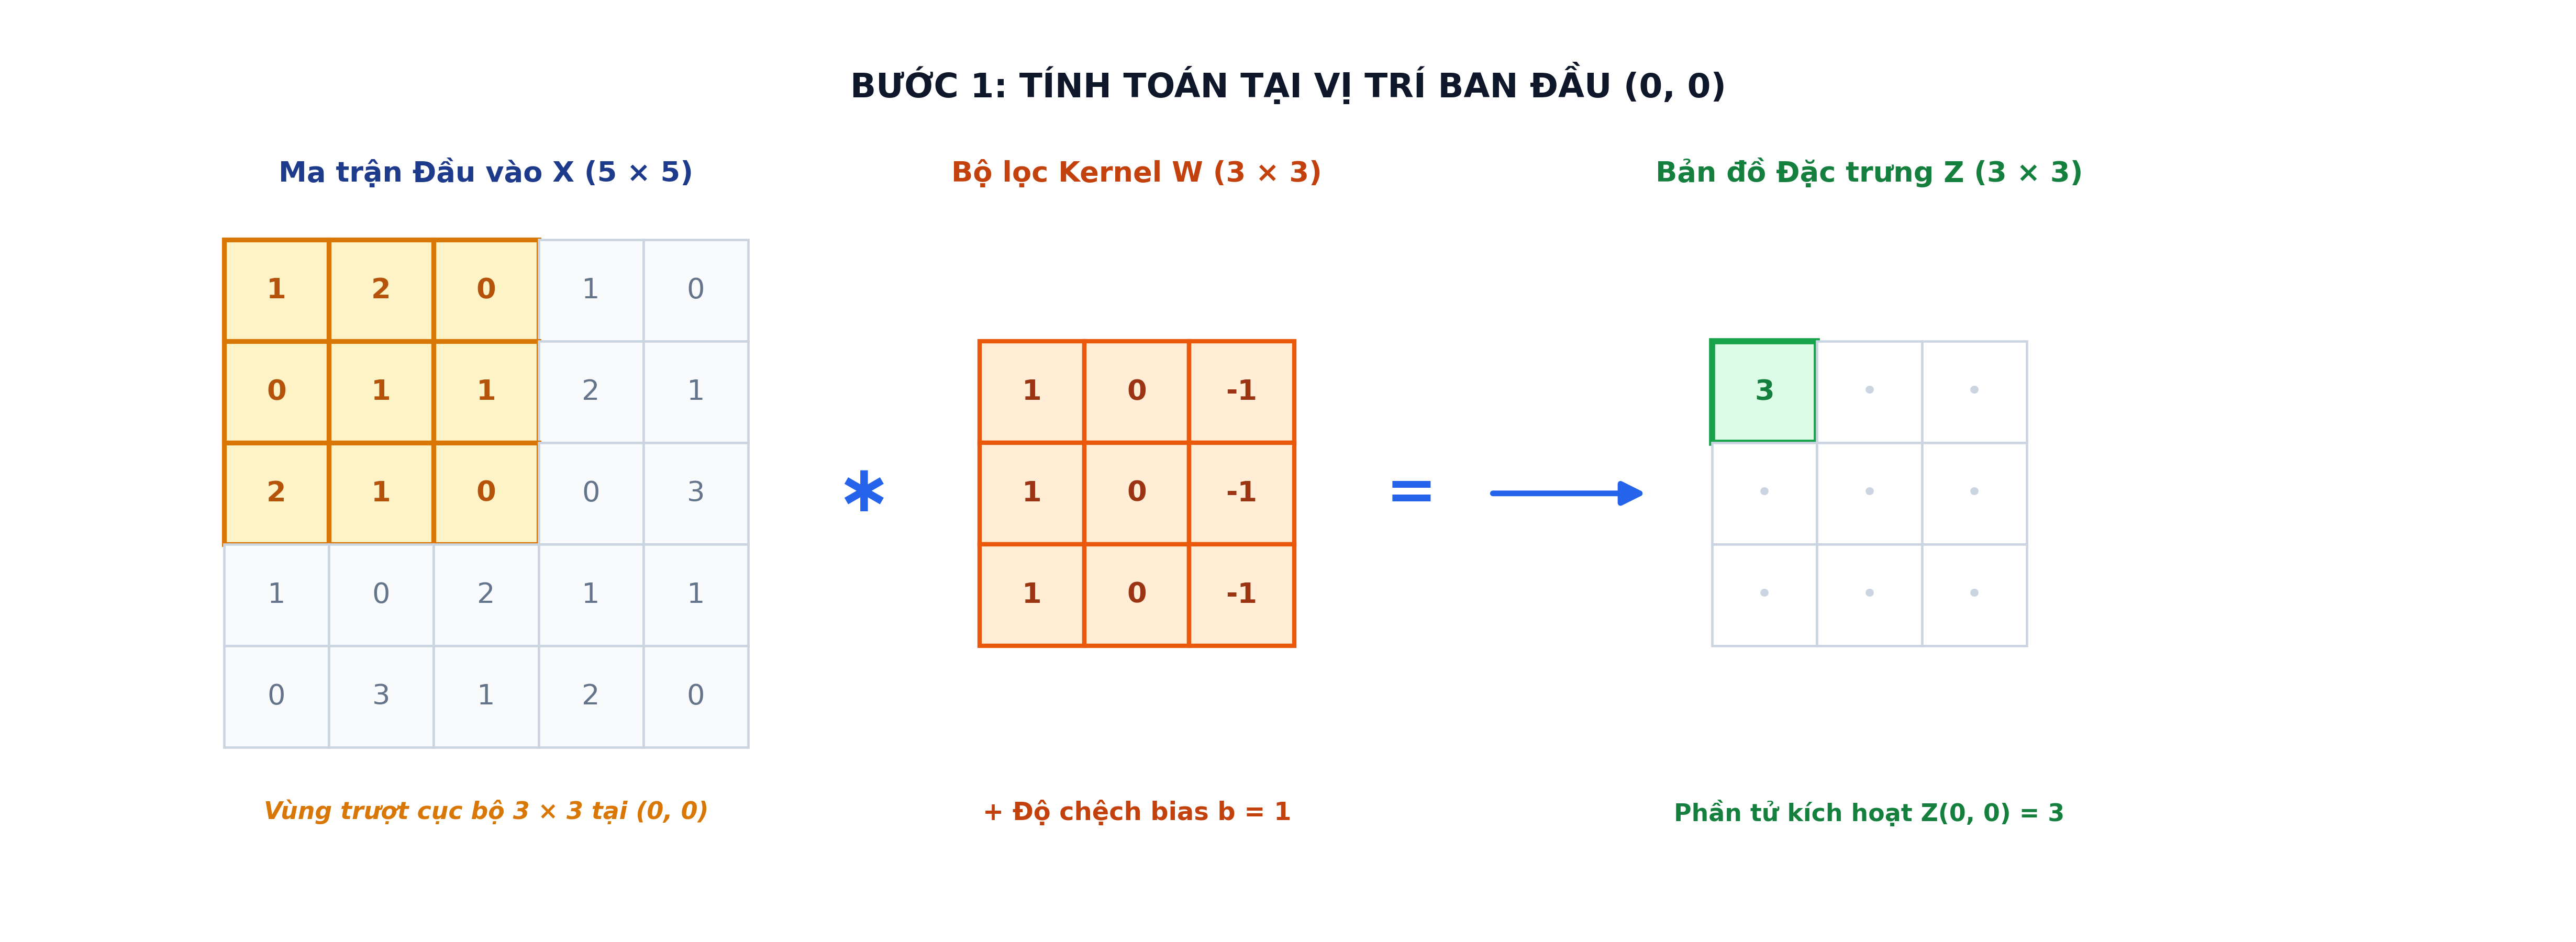
\includegraphics[width=0.80\textwidth]{images/fig06a_conv_step1_pos00.png}
\caption{Phép tích chập 2D tại vị trí ban đầu $(0, 0)$}
\label{fig:numerical_conv_step1}
\end{figure}

\vspace{-0.5em}
\noindent \textbf{Bước 2: Dịch chuyển sang phải một bước trượt ($s = 1$) tới vị trí (0, 1):} \\
Bộ lọc tiếp tục dịch sang phải 1 cột (tương ứng bước trượt Stride $s = 1$), bao phủ vùng cục bộ $\mathbf{X}_{\text{patch}}^{(0, 1)} = \begin{bmatrix} 2 & 0 & 1 \\ 1 & 1 & 2 \\ 1 & 0 & 0 \end{bmatrix}$. Giá trị kích hoạt thô tiếp theo $Z(0, 1)$ được tính:
\begin{align}
Z(0, 1) &= (2 \cdot 1 + 0 \cdot 0 + 1 \cdot (-1)) + (1 \cdot 1 + 1 \cdot 0 + 2 \cdot (-1)) + (1 \cdot 1 + 0 \cdot 0 + 0 \cdot (-1)) + 1 \nonumber\\
&= (2 - 1) + (1 - 2) + (1 - 0) + 1 = 1 - 1 + 1 + 1 = 2
\end{align}
Phần tử $Z(0, 1) = 2$ được cập nhật tiếp vào vị trí tương ứng trên bản đồ đặc trưng đầu ra như thể hiện trong Hình \ref{fig:numerical_conv_step2}.

\begin{figure}[H]
\centering
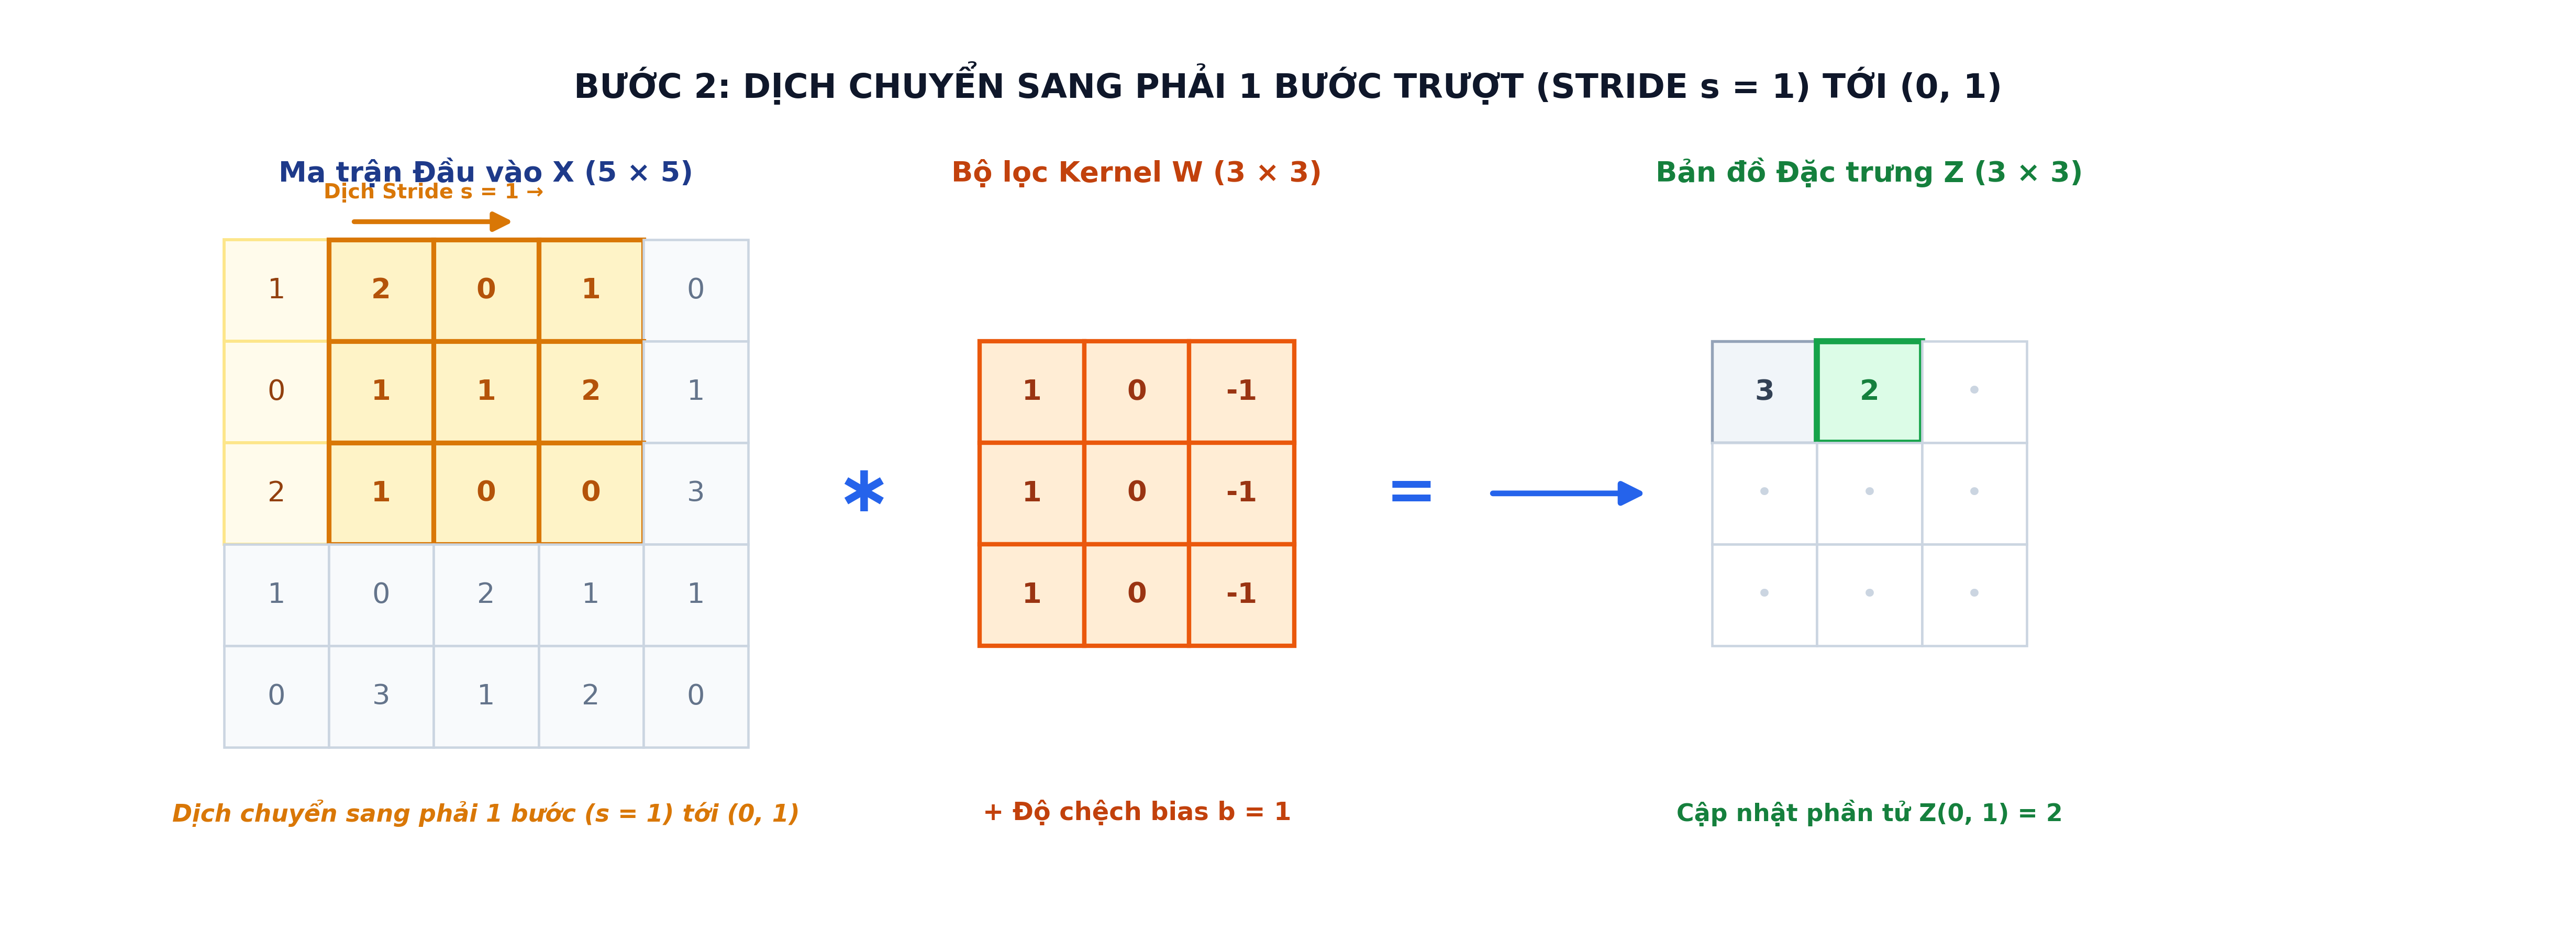
\includegraphics[width=0.80\textwidth]{images/fig06b_conv_step2_pos01.png}
\caption{Phép tích chập 2D khi dịch bước trượt sang phải $(0, 1)$}
\label{fig:numerical_conv_step2}
\end{figure}

\vspace{-0.5em}
\noindent \textbf{Bước 3: Chuyển hàng trượt xuống vị trí (1, 0) \& Hoàn tất bản đồ đặc trưng:} \\
Sau khi quét hết hàng đầu tiên tại $(0, 2)$ cho $Z(0, 2) = -2$, bộ lọc dịch chuyển xuống hàng tiếp theo bắt đầu từ cột 0 tại tọa độ $(1, 0)$, bao phủ vùng ảnh $\mathbf{X}_{\text{patch}}^{(1, 0)} = \begin{bmatrix} 0 & 1 & 1 \\ 2 & 1 & 0 \\ 1 & 0 & 2 \end{bmatrix}$:
\begin{equation}
Z(1, 0) = (0 - 1) + (2 - 0) + (1 - 2) + 1 = -1 + 2 - 1 + 1 = 1
\end{equation}
Lặp lại quy trình trượt tuần tự qua toàn bộ 9 vị trí (3 hàng $\times$ 3 cột), toàn bộ bản đồ đặc trưng đầu ra kích thước $3 \times 3$ được xác định trọn vẹn:
\begin{equation}
\mathbf{Z} = \begin{bmatrix} 3 & 2 & -2 \\ 1 & 0 & -1 \\ 1 & 2 & 0 \end{bmatrix}
\end{equation}

\begin{figure}[H]
\centering
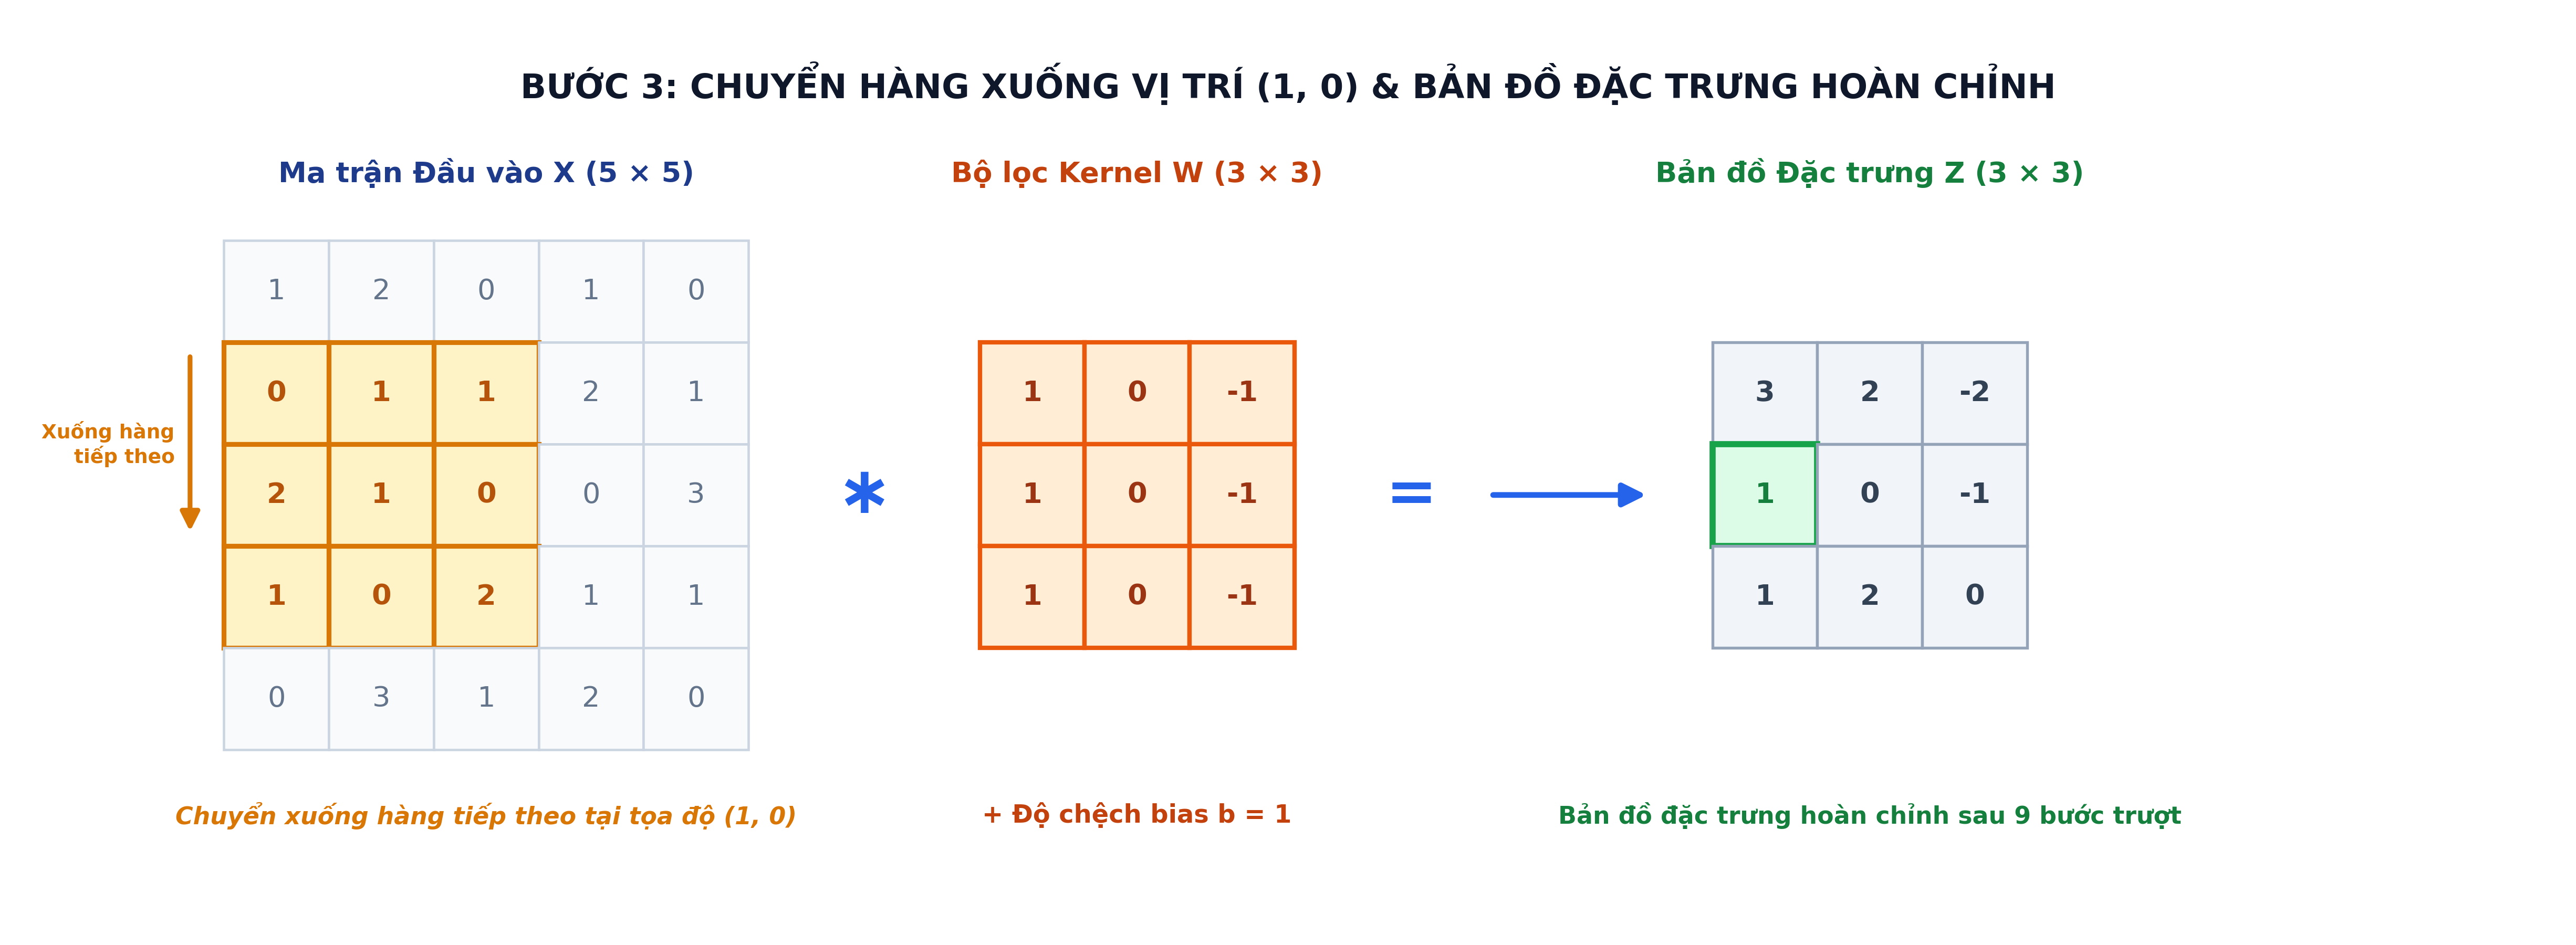
\includegraphics[width=0.80\textwidth]{images/fig06c_conv_step3_complete.png}
\caption{Phép tích chập 2D khi chuyển xuống hàng $(1, 0)$ và kết quả hoàn chỉnh}
\label{fig:numerical_conv_step3}
\end{figure}

\newpage

\subsection{Cơ Chế Gom Kênh Trong Tích Chập 3D Đa Kênh (Multi-Channel Convolution)}
Trong các bài toán thực tế, dữ liệu đầu vào hoặc các bản đồ đặc trưng trung gian luôn có nhiều kênh ($C_{\text{in}} > 1$, ví dụ $C_{\text{in}} = 3$ với ảnh RGB hoặc $C_{\text{in}} = 64$ sau các tầng ẩn). Để xử lý dữ liệu đa kênh, mỗi bộ lọc tích chập bản thân nó là một tensor 3 chiều có cùng độ sâu:
\begin{equation}
\mathbf{W}^{(m)} \in \mathbb{R}^{K_H \times K_W \times C_{\text{in}}}
\end{equation}
Quy trình gom kênh diễn ra qua 3 pha tuần tự:
\begin{enumerate}[leftmargin=1.5em]
    \item \textbf{Tích chập đơn kênh đồng thời:} Kernel trên mỗi kênh $c \in \{1, \dots, C_{\text{in}}\}$ thực hiện phép tích chập 2D trên kênh ảnh tương ứng, sinh ra $C_{\text{in}}$ ma trận kết quả trung gian.
    \item \textbf{Cộng tổng theo chiều sâu (Depth-wise Summation):} Toàn bộ $C_{\text{in}}$ ma trận trung gian này được cộng dồn theo từng tọa độ không gian $(i, j)$:
    \begin{equation}
    Z(i, j, m) = \sum_{c=1}^{C_{\text{in}}} \left( \mathbf{X}_{:, :, c} * \mathbf{W}_{:, :, c}^{(m)} \right)(i, j) + b(m)
    \end{equation}
    Phép cộng dồn này tổng hợp toàn bộ thông tin từ các phổ màu hoặc các đặc trưng khác nhau thành \textbf{một bản đồ đặc trưng 2D duy nhất}.
    \item \textbf{Tập hợp $M$ bộ lọc:} Nếu tầng tích chập sở hữu $M$ bộ lọc độc lập, ta sẽ thu được chính xác $M$ bản đồ đặc trưng 2D, xếp chồng lên nhau tạo thành tensor 3D đầu ra $\mathbf{Z} \in \mathbb{R}^{H_{\text{out}} \times W_{\text{out}} \times M}$.
\end{enumerate}

\begin{figure}[H]
\centering
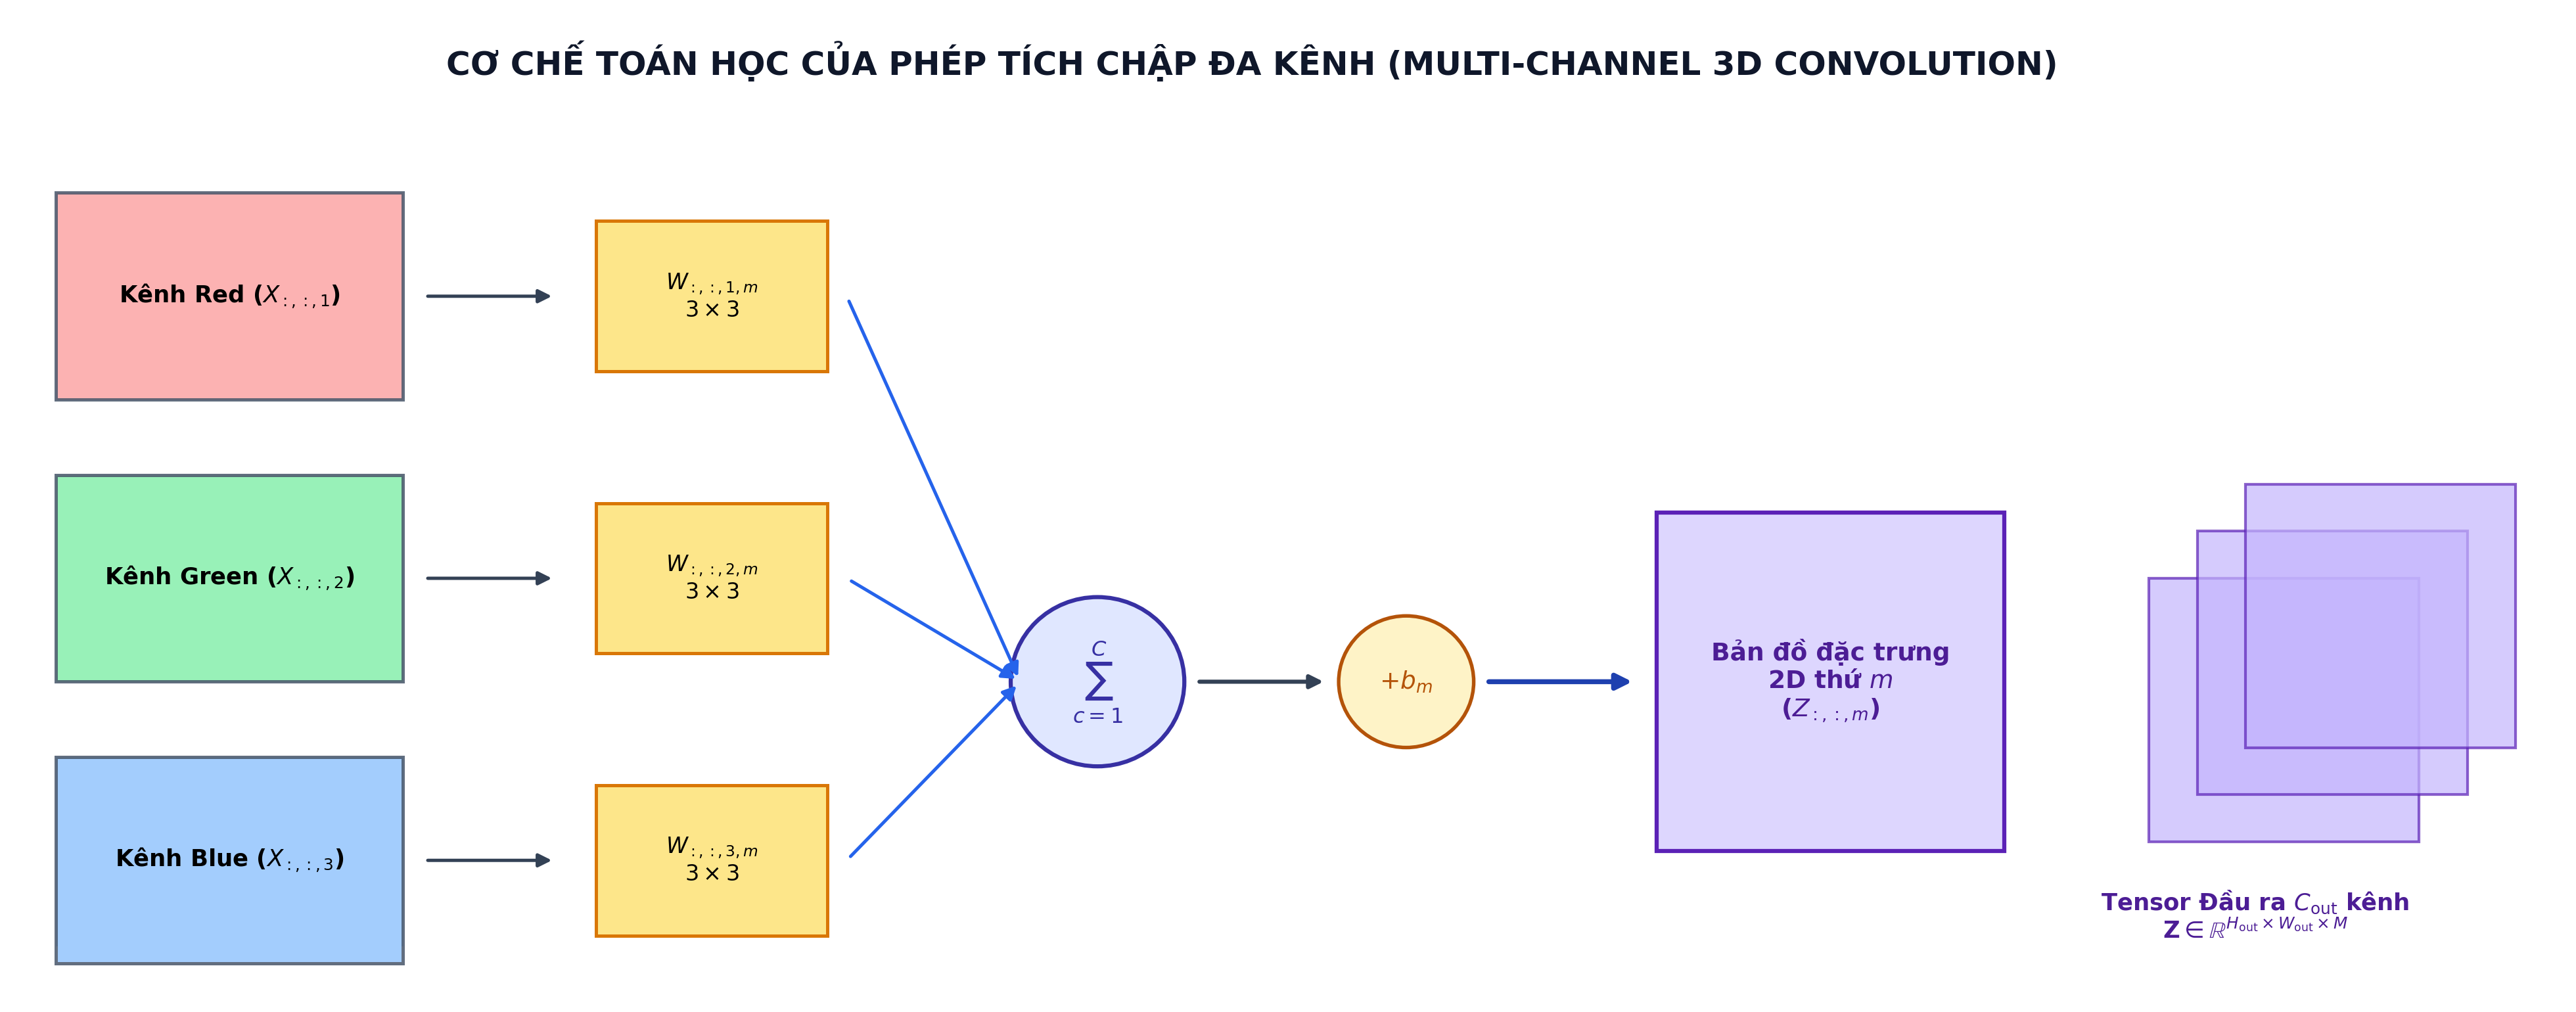
\includegraphics[width=0.96\textwidth]{images/fig02_multichannel_convolution_detailed.png}
\caption{Cơ chế tích chập đa kênh (Multi-Channel Convolution)}
\label{fig:multichannel_conv}
\end{figure}

\newpage

\section{Các Siêu Tham Số Hình Học Điều Khiển Không Gian}

Kích thước không gian của bản đồ đặc trưng đầu ra được kiểm soát và định hình bởi ba siêu tham số kỹ thuật cốt lõi:

\subsection{Đệm Viền (Zero-Padding -- $P$)}
Khi quét kernel trên ảnh không đệm, các điểm ảnh ở góc viền ngoài cùng chỉ được bộ lọc quét qua 1 lần duy nhất, trong khi các điểm ảnh ở trung tâm được quét tới $K^2$ lần. Điều này dẫn đến hai hệ quả bất lợi: kích thước ảnh bị thu hẹp dần sau mỗi tầng và thông tin ở vùng biên bị suy giảm nghiêm trọng. Kỹ thuật Zero-Padding giải quyết vấn đề này bằng cách chèn thêm $P$ hàng và cột số 0 bao quanh biên ngoài của ảnh:
\begin{itemize}[leftmargin=2em]
    \item \textbf{Valid Padding ($P = 0$):} Không đệm viền. Kích thước bản đồ đặc trưng giảm dần: $H_{\text{out}} = H_{\text{in}} - K + 1$. Sau một vài tầng tích chập sâu, kích thước ảnh sẽ tiêu biến về 0.
    \item \textbf{Same Padding ($P = \lfloor K/2 \rfloor$ với bước trượt $s=1$):} Đệm viền sao cho kích thước không gian đầu ra bằng đúng đầu vào ($H_{\text{out}} = H_{\text{in}}$). Đây là cơ sở then chốt cho phép xây dựng các mạng nơ-ron hiện đại sâu hàng chục tầng (như VGG, ResNet).
\end{itemize}

\begin{figure}[H]
\centering
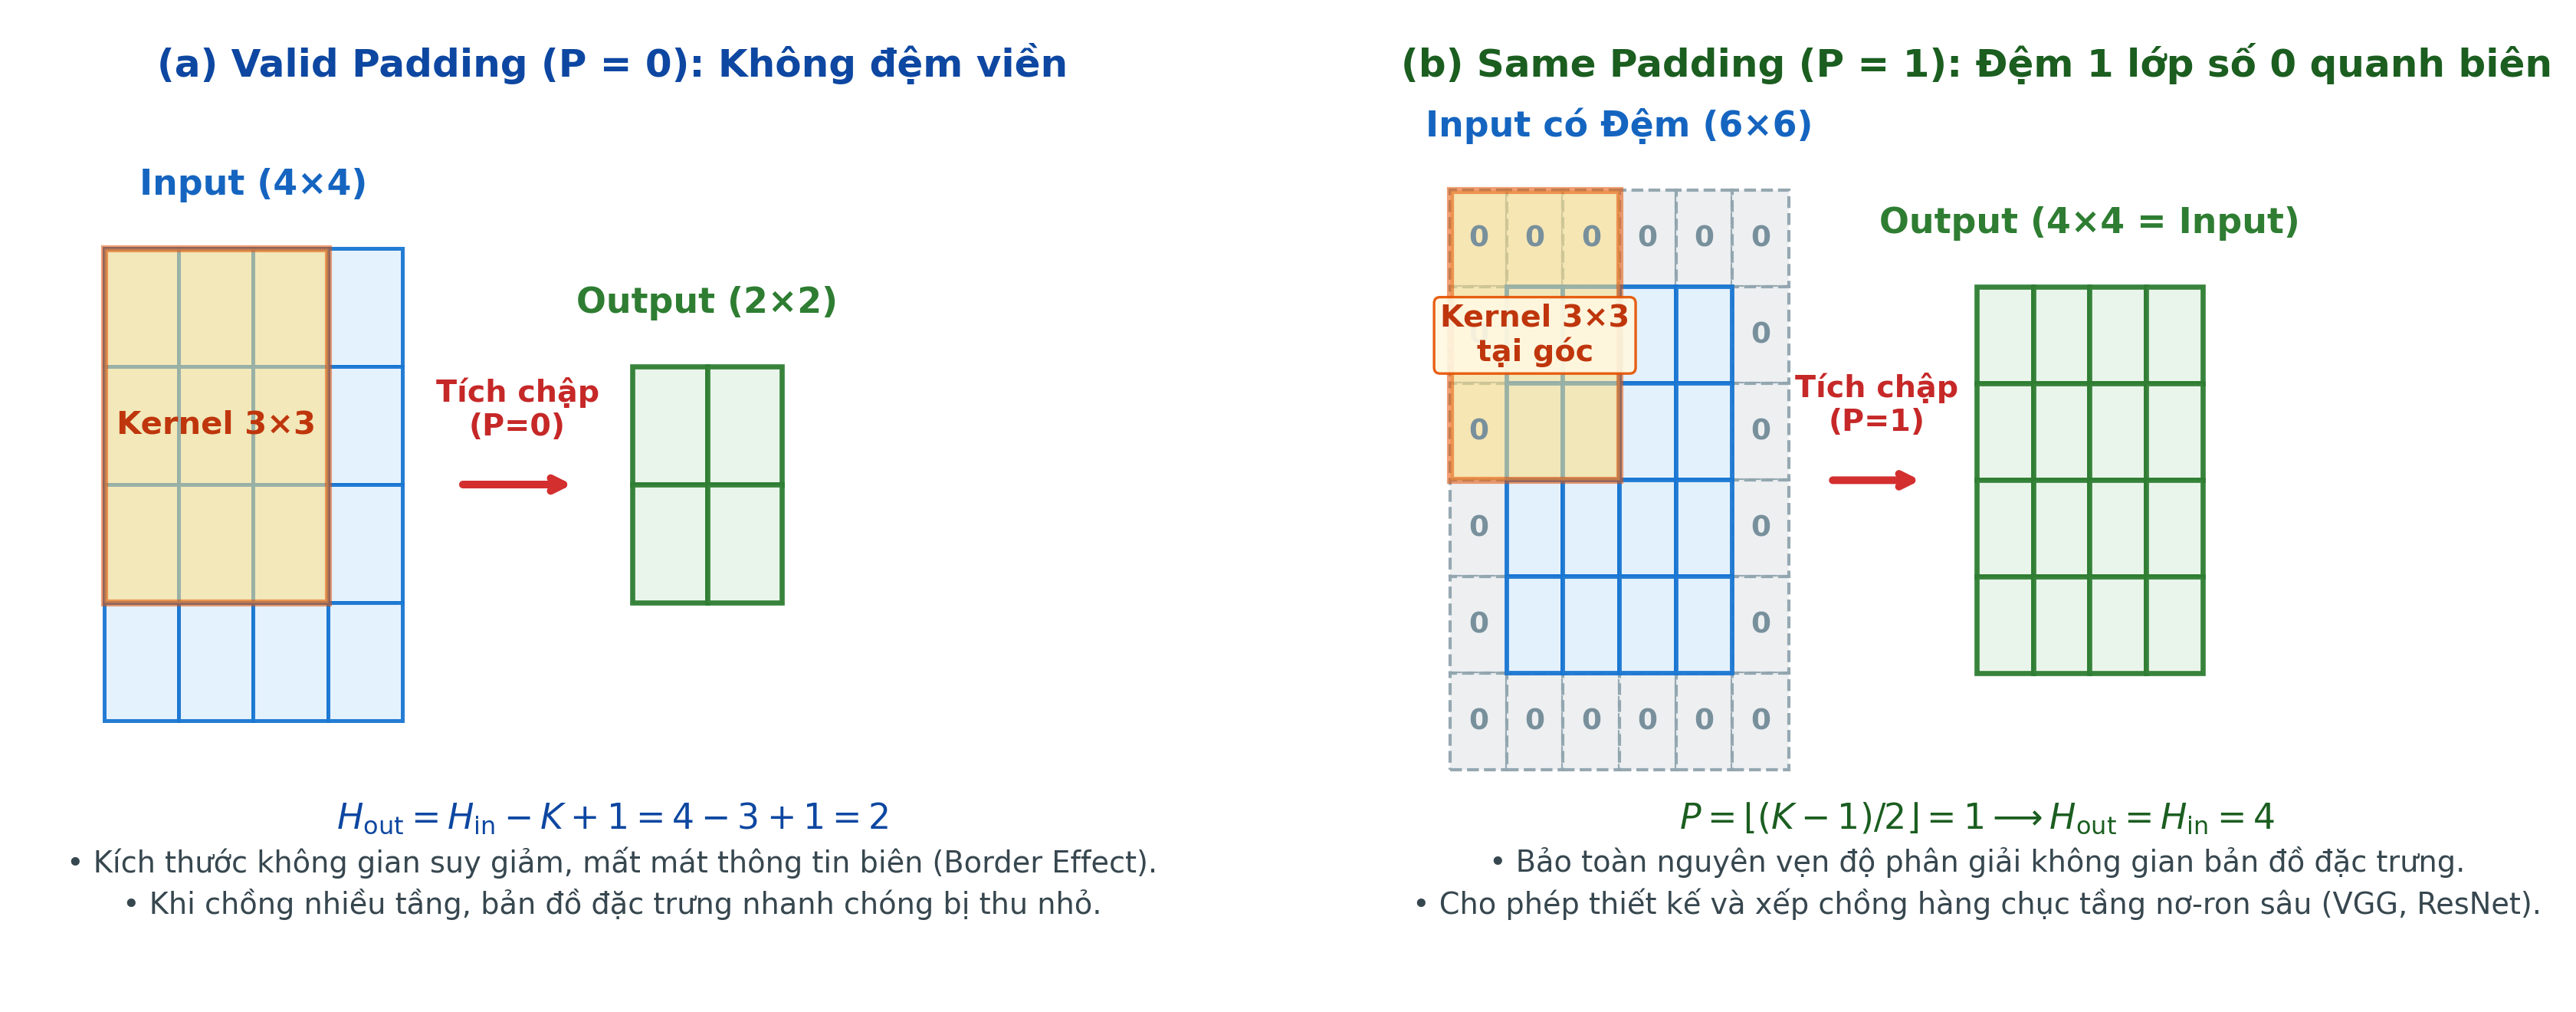
\includegraphics[width=0.92\textwidth]{images/theory_zero_padding.png}
\caption{So sánh cơ chế đệm viền Valid Padding và Same Padding}
\label{fig:zero_padding}
\end{figure}

\newpage

\subsection{Bước Trượt (Stride -- $s$)}
Bước trượt $s$ biểu thị số lượng điểm ảnh mà kernel dịch chuyển trên ảnh sau mỗi lần tính toán:
\begin{itemize}[leftmargin=2em]
    \item \textbf{Stride $s = 1$:} Cửa sổ trượt dịch chuyển từng điểm ảnh một. Tín hiệu được quét với độ phân giải mịn tối đa, bảo toàn vị trí chính xác của từng chi tiết nhỏ.
    \item \textbf{Stride $s = 2$:} Cửa sổ trượt nhảy cách quãng 2 điểm ảnh mỗi bước. Kích thước không gian của bản đồ đặc trưng đầu ra bị giảm đi một nửa ($H_{\text{out}} \approx H_{\text{in}} / 2$). Stride $s=2$ đóng vai trò như một cơ chế giảm mẫu không gian có khả năng học được (Learned Downsampling), thường được dùng thay thế cho Pooling trong các kiến trúc nơ-ron hiện đại.
\end{itemize}

\begin{figure}[H]
\centering
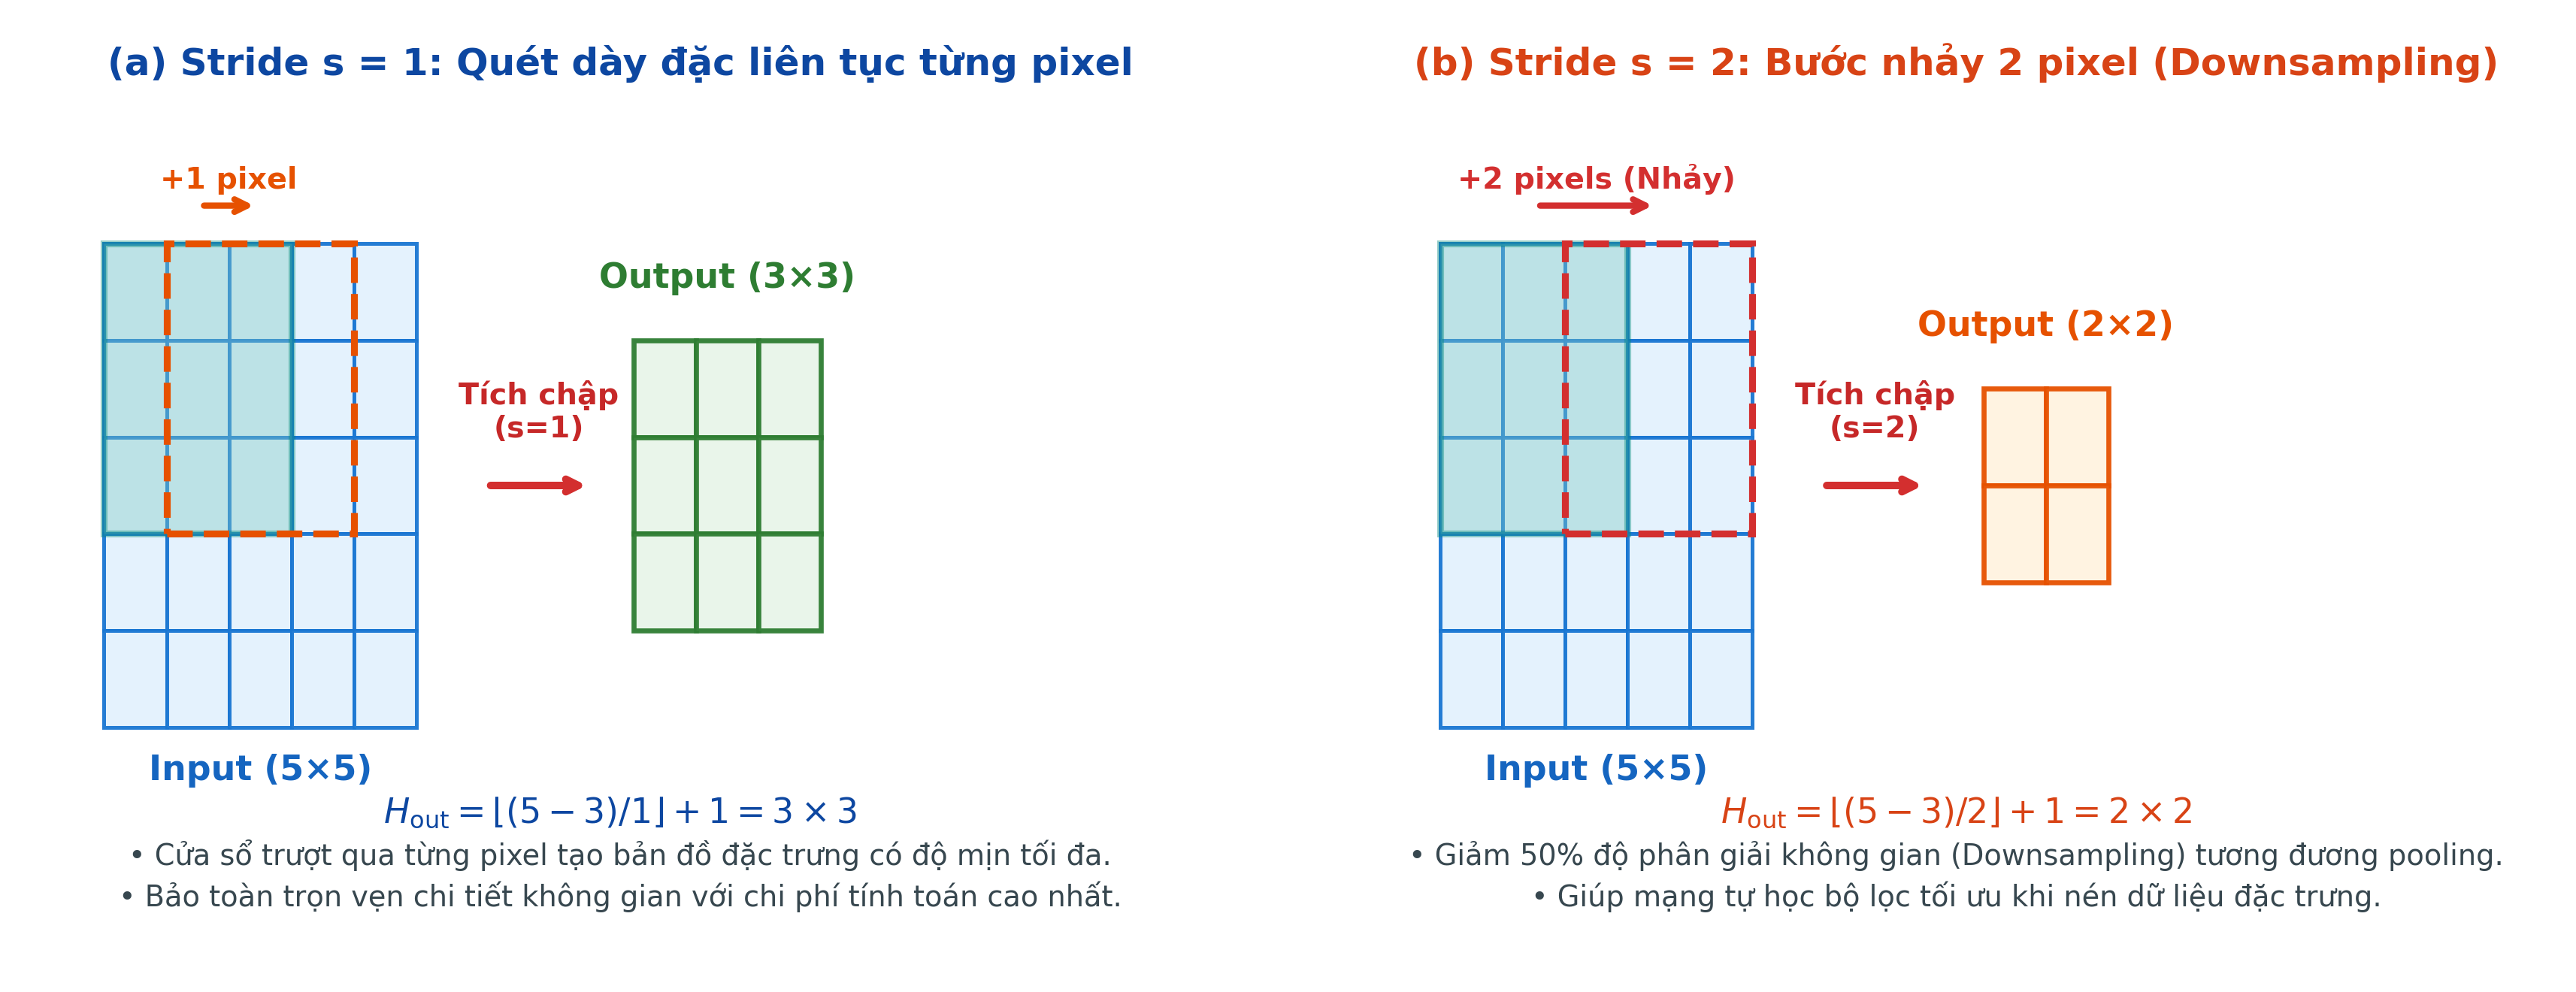
\includegraphics[width=0.92\textwidth]{images/theory_stride.png}
\caption{Cơ chế bước trượt (Stride) với $s=1$ và $s=2$}
\label{fig:stride}
\end{figure}

\subsection{Độ Giãn Nở (Dilation Rate -- $d$)}
Tích chập giãn nở (Dilated / Atrous Convolution) chèn thêm $(d - 1)$ khoảng trống có giá trị 0 vào giữa các trọng số liền kề của kernel:
\begin{equation}
K' = K + (K - 1)(d - 1)
\end{equation}
Khi $d = 2$, một kernel $3 \times 3$ thông thường sẽ mở rộng phạm vi bao phủ không gian tương đương với một vùng $5 \times 5$, nhưng vẫn chỉ tiêu tốn đúng 9 tham số trọng số. Kỹ thuật này giúp mở rộng theo cấp số nhân vùng quan sát thị giác (Receptive Field) mà không làm tăng số lượng tham số hay suy giảm độ phân giải không gian, là trụ cột trong các bài toán phân đoạn ngữ nghĩa ảnh (Semantic Segmentation).

\begin{figure}[H]
\centering
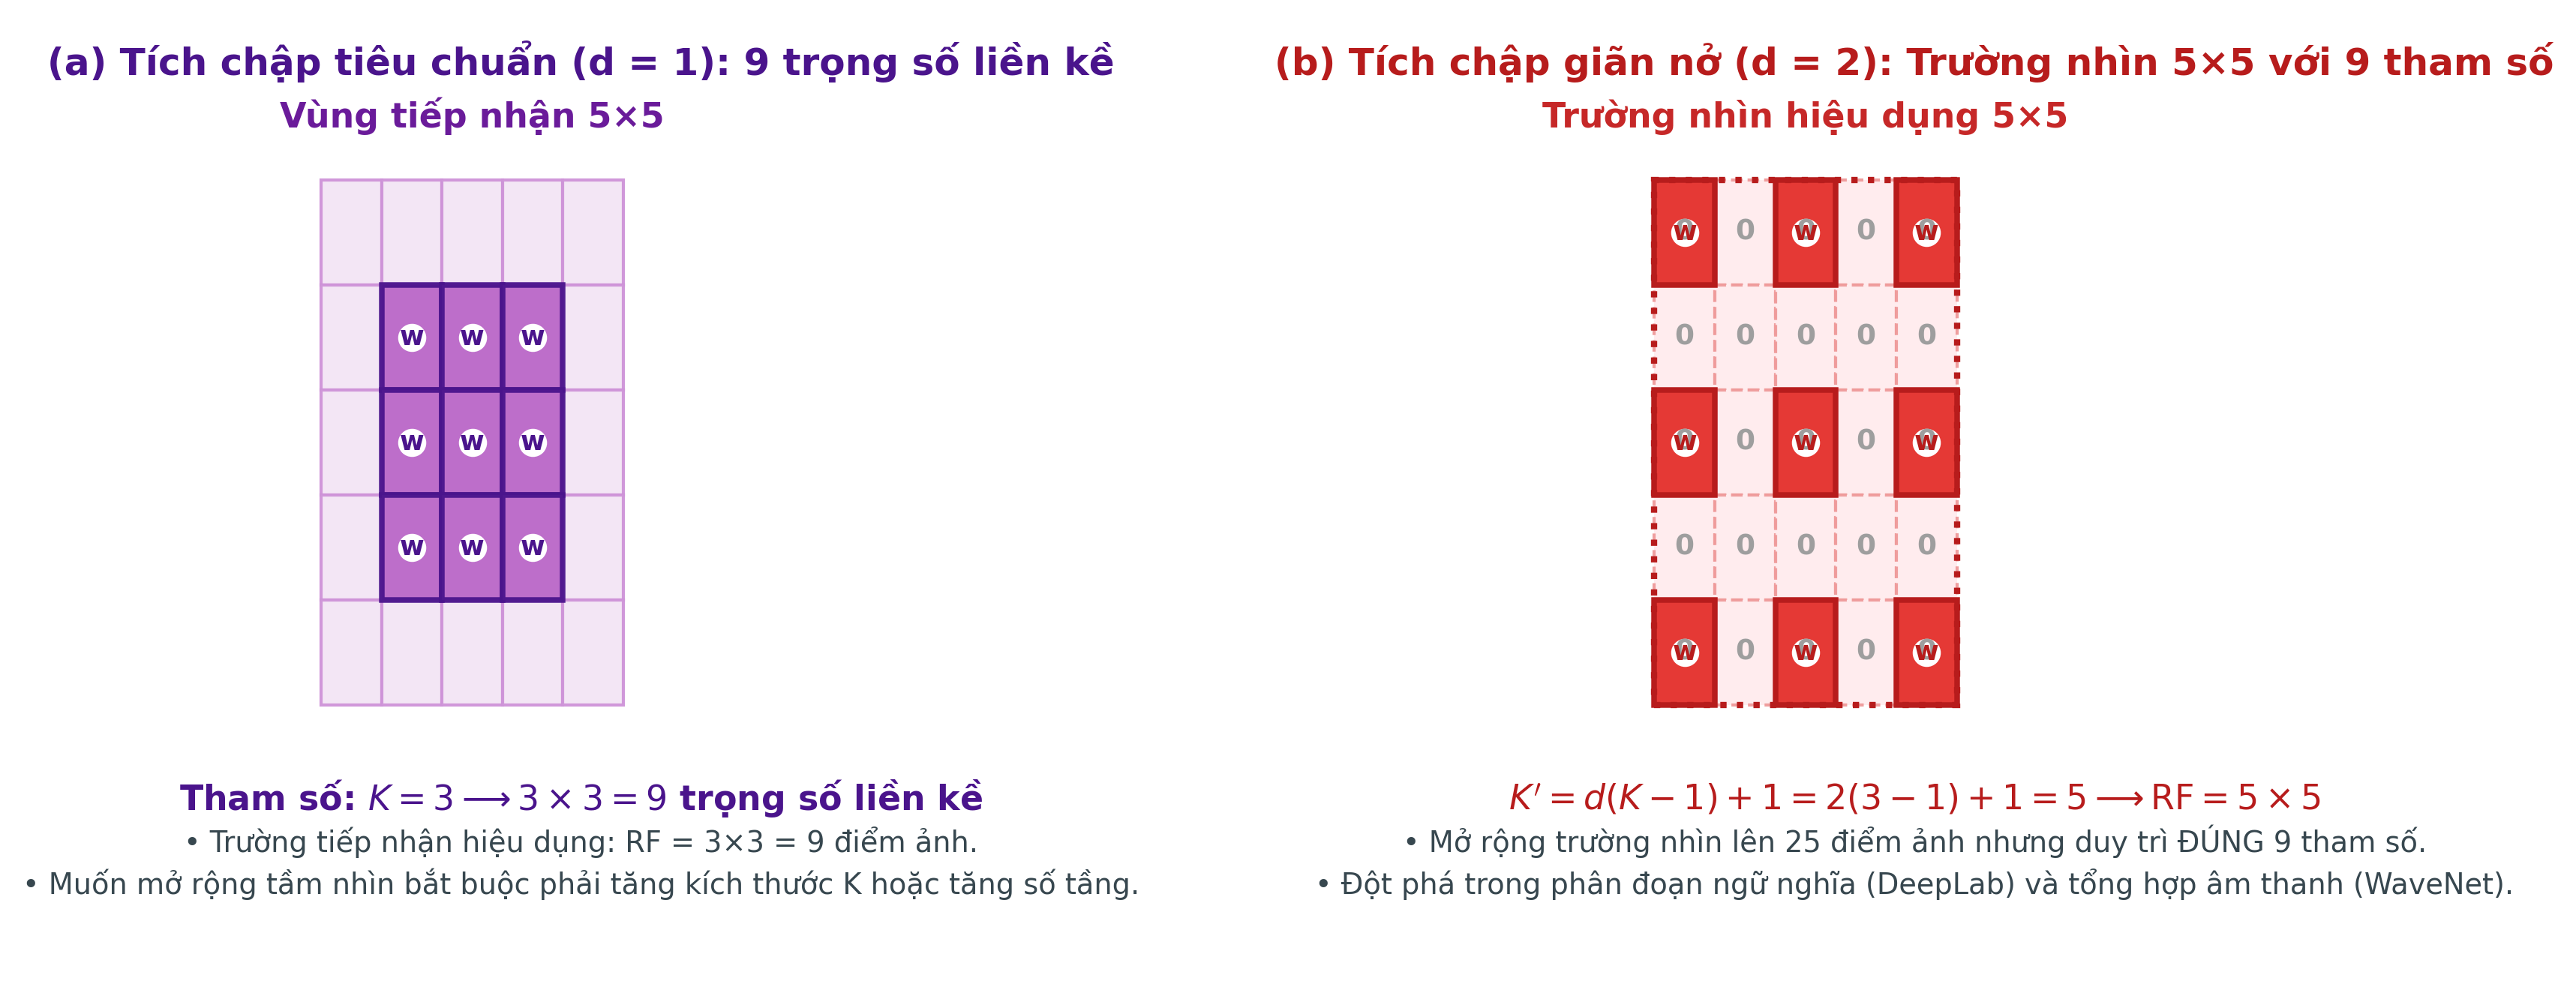
\includegraphics[width=0.70\textwidth]{images/theory_dilation.png}
\caption{Cơ chế tích chập giãn nở (Dilated Convolution)}
\label{fig:dilation}
\end{figure}

\subsection{Công Thức Tổng Quát Xác Định Kích Thước Không Gian Đầu Ra}
Tổng hợp ảnh hưởng của ba siêu tham số hình học trên, kích thước không gian $(H_{\text{out}}, W_{\text{out}})$ của bản đồ đặc trưng đầu ra được xác định chính xác bởi công thức giải tích:
\begin{equation}
H_{\text{out}} = \left\lfloor \frac{H_{\text{in}} + 2P - d(K_H - 1) - 1}{s} \right\rfloor + 1, \quad
W_{\text{out}} = \left\lfloor \frac{W_{\text{in}} + 2P - d(K_W - 1) - 1}{s} \right\rfloor + 1
\label{eq:output_shape_formula}
\end{equation}

\section{Trường Tiếp Nhận (Receptive Field) \& Nguyên Lý Thừa Số Hóa Bộ Lọc}

\subsection{Định Nghĩa Trường Tiếp Nhận Hiệu Dụng (Receptive Field)}
Trường tiếp nhận (Receptive Field -- RF) của một nơ-ron tại tầng thứ $l$ là diện tích vùng không gian trên ảnh đầu vào ban đầu mà nơ-ron đó có khả năng ``quan sát'' và chịu ảnh hưởng trực tiếp (Hình~\ref{fig:rf_definition}). Ở tầng tích chập đầu tiên với kernel $3 \times 3$, mỗi nơ-ron chỉ nhìn thấy vùng $3 \times 3$ trên ảnh gốc. Khi qua chuỗi các tầng kế tiếp, trường tiếp nhận sẽ tích lũy và mở rộng phân tầng theo công thức giải tích $RF_l = RF_{l-1} + (K_l - 1)$, cho phép một nơ-ron đơn lẻ tại tầng sâu nắm bắt được ngữ cảnh không gian toàn cục rộng lớn của ảnh gốc.

\begin{figure}[H]
\centering
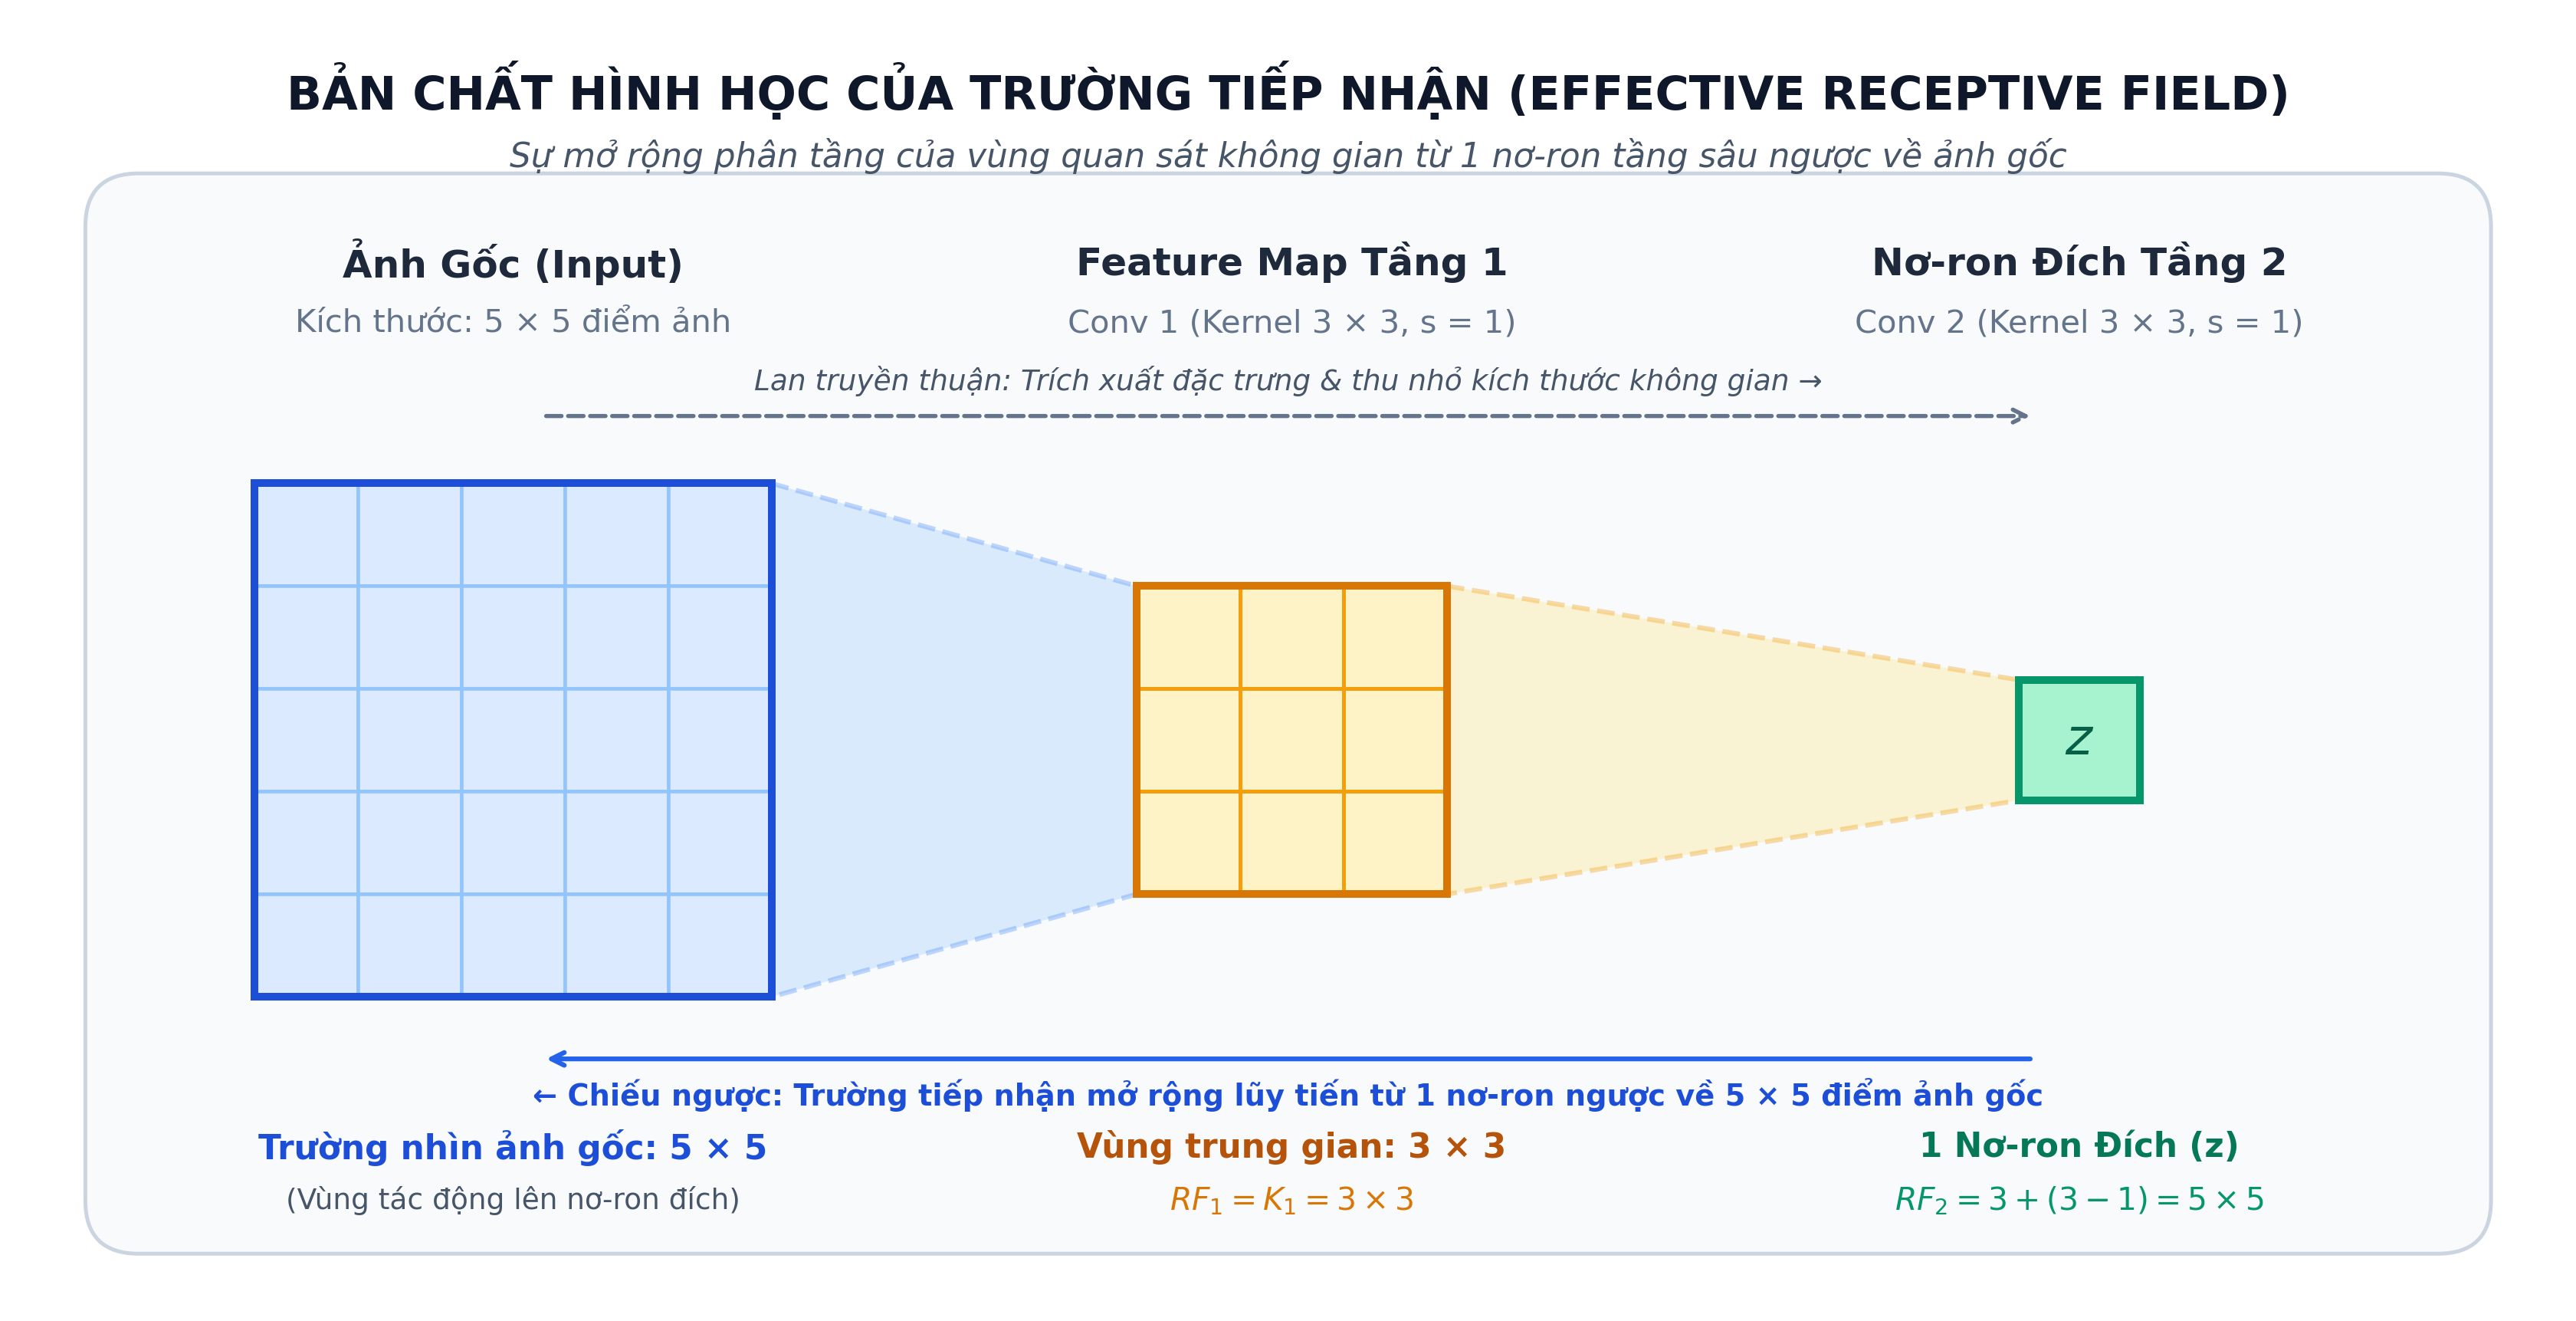
\includegraphics[width=0.82\textwidth]{images/fig_receptive_field_definition.png}
\caption{Mô hình hình học trường tiếp nhận hiệu dụng (Receptive Field)}
\label{fig:rf_definition}
\end{figure}

\newpage

\subsection{Nguyên Lý Thừa Số Hóa Bộ Lọc (Filter Factorization)}
Trong nghiên cứu kiến trúc mạng VGGNet kinh điển (Simonyan \& Zisserman, 2014), một nguyên lý đột phá đã được chứng minh: \textbf{Xếp chồng chuỗi ba tầng tích chập $3 \times 3$ liên tiếp tạo ra trường tiếp nhận hiệu dụng tương đương đúng một tầng tích chập lớn $7 \times 7$}.
\begin{itemize}[leftmargin=1.8em, itemsep=3pt, parsep=0pt]
    \item \textbf{Cơ chế hình học kim tự tháp:} Với bước trượt $s=1$, trường tiếp nhận tích lũy theo công thức $RF_l = RF_{l-1} + (K_l - 1)$. Tầng 1 đạt $RF_1 = 3 \times 3$, Tầng 2 mở rộng $RF_2 = 3 + (3 - 1) = 5 \times 5$, và Tầng 3 bao trọn $RF_3 = 5 + (3 - 1) = 7 \times 7$. Chỉ một nơ-ron tại tầng 3 đã có khả năng bao quát toàn bộ vùng $7 \times 7$ điểm ảnh trên ảnh gốc.
    \item \textbf{Tiết kiệm 45\% tham số trọng số:} Một tầng $7 \times 7$ với $C$ kênh tiêu tốn $1 \times (7^2 \cdot C^2) = 49 C^2$ tham số; trong khi ba tầng $3 \times 3$ chỉ tiêu tốn $3 \times (3^2 \cdot C^2) = 27 C^2$ tham số. Tỷ lệ tham số $\frac{27 C^2}{49 C^2} \approx 55.1\% \implies$ Cắt giảm đến $\mathbf{45\%}$ dung lượng mô hình.
    \item \textbf{Gấp 3 lần năng lực phi tuyến (Triple ReLU):} Thay vì chỉ có 1 hàm ReLU sau tầng $7 \times 7$, cấu trúc 3 tầng $3 \times 3$ chèn xen kẽ 3 hàm kích hoạt ReLU liên tiếp, giúp mạng học được các hàm xấp xỉ sâu và trừu tượng hơn vượt bậc.
\end{itemize}

\begin{figure}[H]
\centering
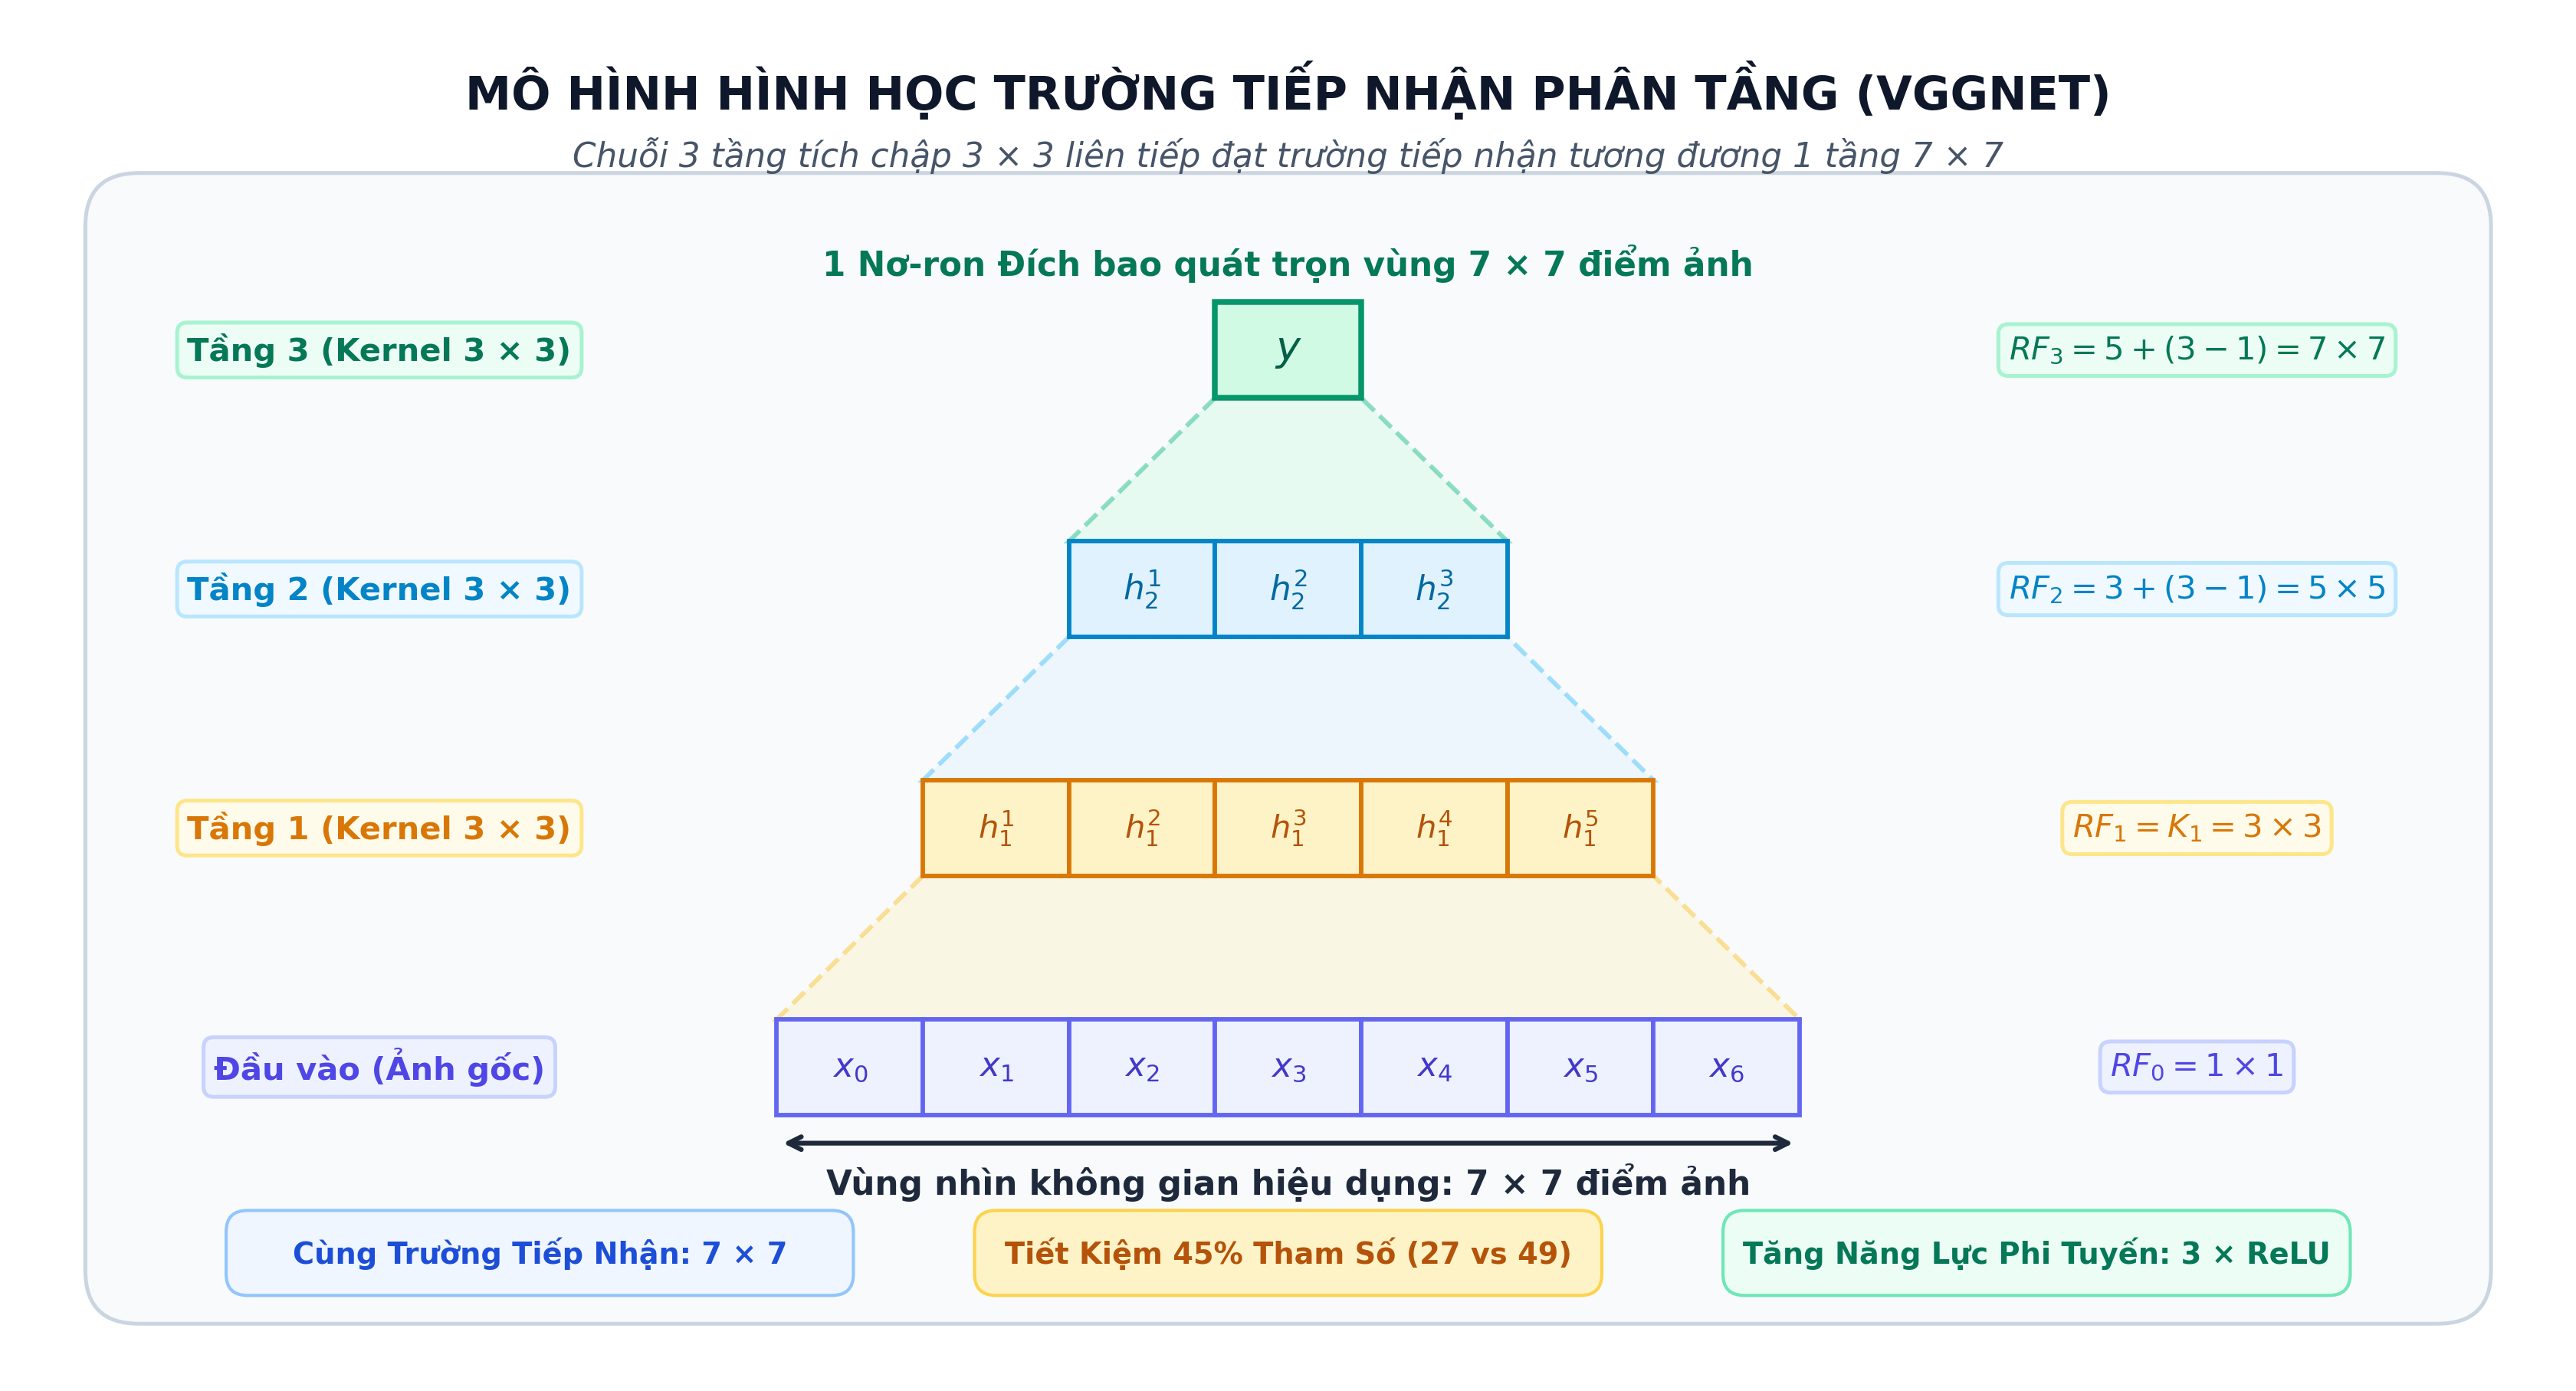
\includegraphics[width=0.92\textwidth]{images/fig07_receptive_field_stacking.png}
\caption{Nguyên lý thừa số hóa bộ lọc trong kiến trúc VGGNet}
\label{fig:receptive_field}
\end{figure}

\newpage

\section{Hàm Kích Hoạt Phi Tuyến (Nonlinear Activation)}

\subsection{Vai Trò Bắt Buộc Của Tính Phi Tuyến}
Phép tích chập thuần túy bản chất là một phép biến đổi tuyến tính (nhân ma trận). Nếu không có hàm kích hoạt phi tuyến chèn giữa các tầng, một chuỗi $L$ phép tích chập liên tiếp sẽ suy biến về một phép biến đổi tuyến tính duy nhất:
\begin{equation}
\mathbf{W}_L \cdot (\mathbf{W}_{L-1} \dots (\mathbf{W}_1 \mathbf{X})) = \mathbf{W}_{\text{total}} \cdot \mathbf{X}
\end{equation}
Khi đó, toàn bộ mạng sâu dù có hàng trăm tầng cũng chỉ tương đương với một mô hình hồi quy tuyến tính đơn giản, hoàn toàn bất lực trước việc phân loại các mẫu phi tuyến phức tạp trong không gian ảnh.

\subsection{So Sánh Giải Tích: ReLU vs Sigmoid / Tanh \& Vấn Đề Triệt Tiêu Gradient}
Trong các mô hình học sâu hiện đại, hàm \textbf{ReLU (Rectified Linear Unit)} đã thay thế hoàn toàn các hàm bão hòa truyền thống như Sigmoid và Tanh:
\begin{equation}
\text{ReLU}(z) = \max(0, z), \quad \frac{d}{dz}\text{ReLU}(z) = \begin{cases} 1 & \text{khi } z > 0 \\ 0 & \text{khi } z \le 0 \end{cases}
\end{equation}
So sánh giải tích làm nổi bật ba ưu thế áp đảo của ReLU:
\begin{enumerate}[leftmargin=1.5em]
    \item \textbf{Triệt tiêu hiện tượng suy biến gradient (Vanishing Gradient):} Với hàm Sigmoid $\sigma(z) = \frac{1}{1 + e^{-z}}$, đạo hàm cực đại tại $z = 0$ chỉ đạt $0.25$. Khi truyền ngược qua $L$ tầng, gradient suy giảm theo cấp số nhân: $(0.25)^L \to 0$. Hậu quả là các tầng tích chập đầu tiên gần như ngừng học. Ngược lại, đạo hàm của ReLU bằng hằng số $1$ trên toàn bộ miền dương ($z > 0$), cho phép dòng gradient chảy thẳng thông suốt về các tầng sâu nhất.
    \item \textbf{Tối ưu hóa tốc độ tính toán:} ReLU chỉ yêu cầu một phép so sánh ngưỡng $z > 0$, trong khi Sigmoid và Tanh đòi hỏi các phép tính lũy thừa và phân số tốn kém thời gian phần cứng.
    \item \textbf{Tính thưa thớt biểu diễn (Sparse Representation):} Với mọi giá trị âm, ReLU triệt tiêu đầu ra về đúng $0$. Điều này tạo ra biểu diễn thưa tự nhiên (khoảng $50\%$ nơ-ron ở trạng thái nghỉ), mô phỏng cơ chế phản xạ sinh học hiệu quả năng lượng của não bộ.
\end{enumerate}

\begin{figure}[H]
\centering
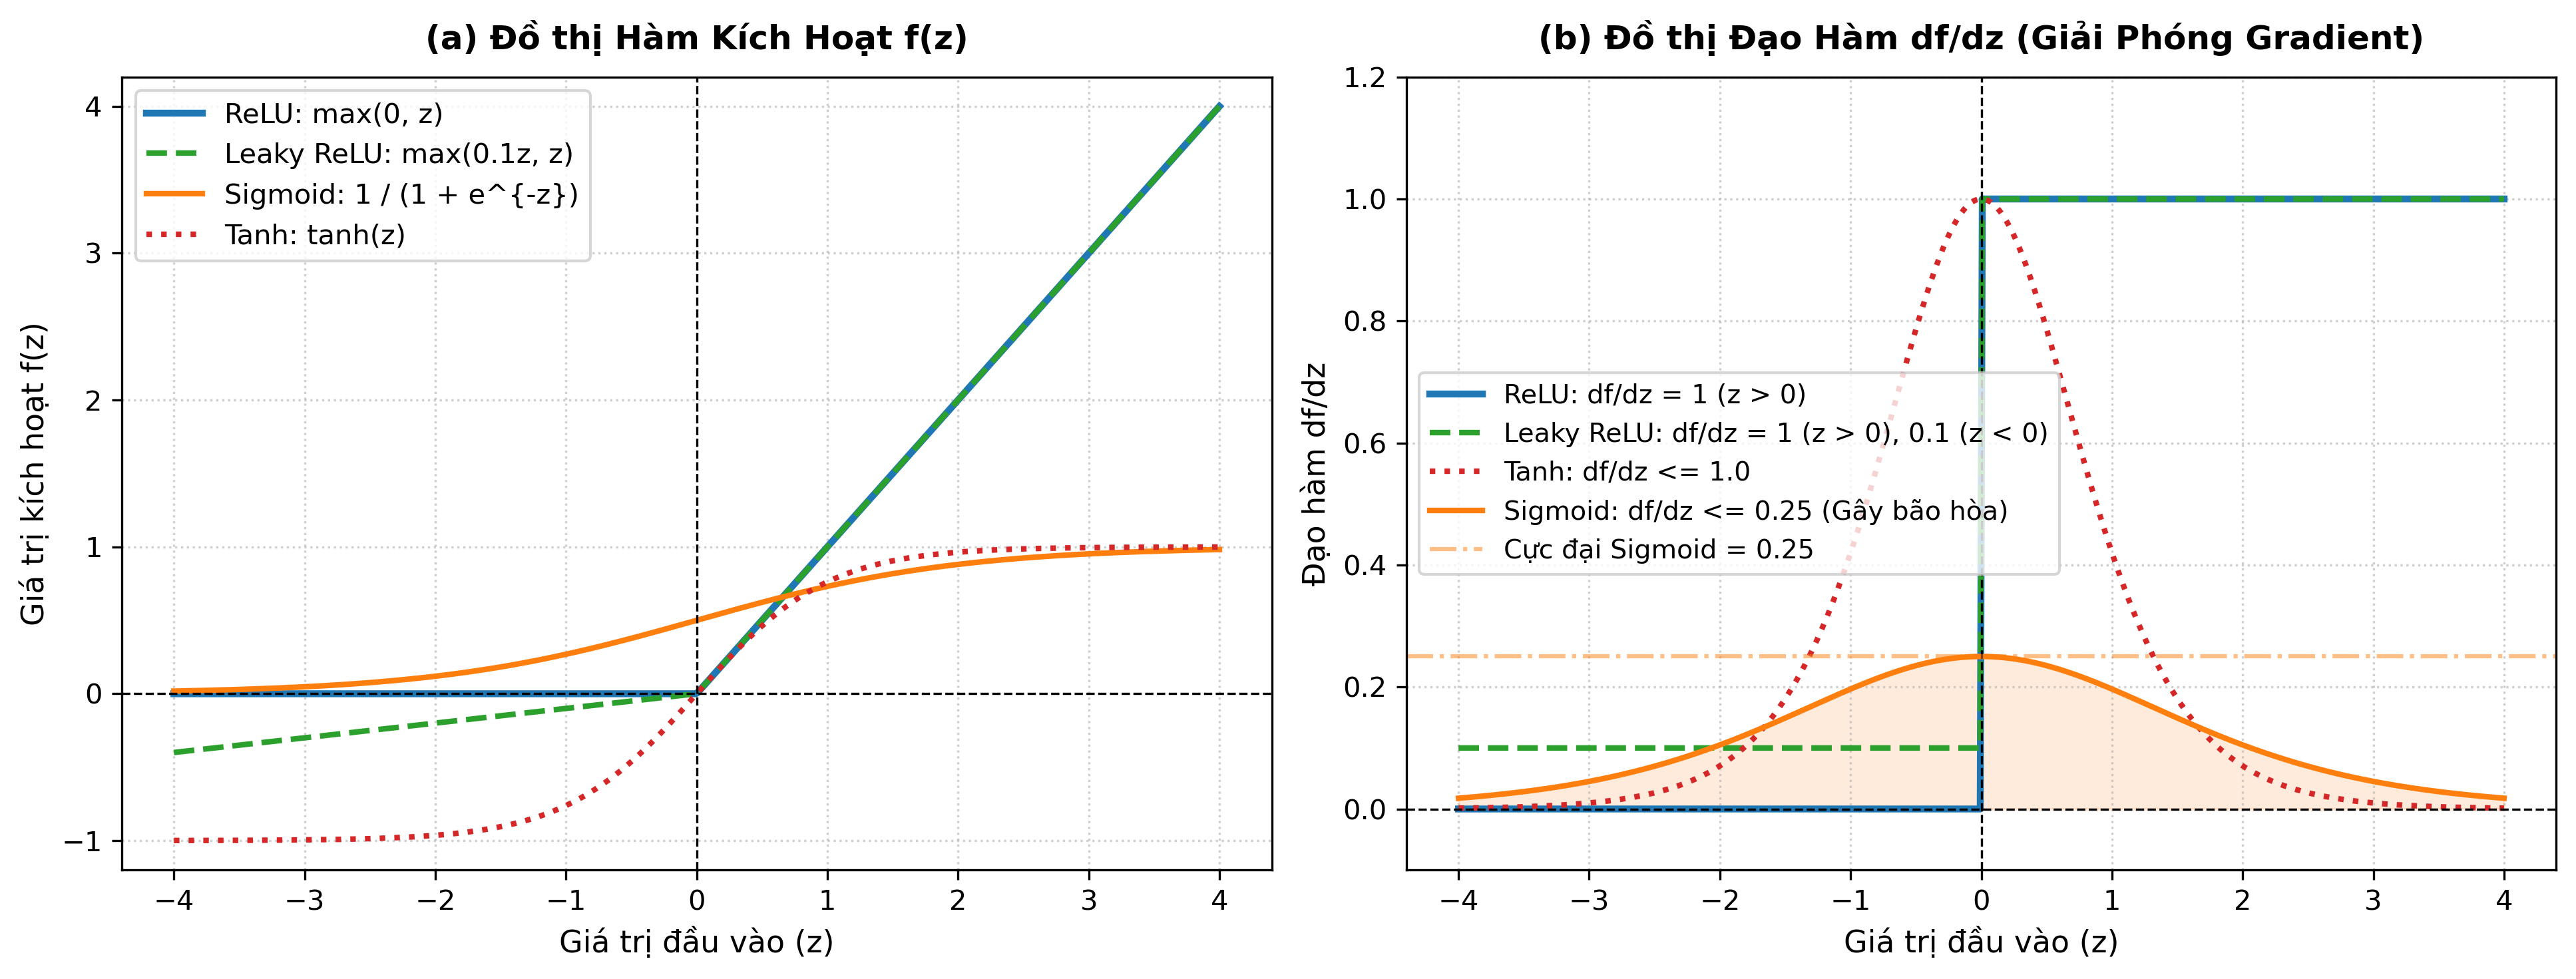
\includegraphics[width=0.92\textwidth]{images/fig08_activation_functions_relu.png}
\caption{Đồ thị hàm số và đạo hàm của ReLU, Leaky ReLU và Sigmoid}
\label{fig:activation_relu}
\end{figure}

\newpage

\section{Hai Cơ Chế Gom Cụm Không Gian: Max Pooling vs GAP}

Nhằm trích xuất các đặc trưng có tính bất biến và tinh gọn không gian biểu diễn, hai kỹ thuật gom cụm đóng vai trò then chốt:

\subsection{Hàm Gom Cụm Cực Đại (Max Pooling)}
Hàm Max Pooling quét một cửa sổ kích thước $K_p \times K_p$ (chuẩn mực là $2 \times 2$ với bước trượt $s=2$) trên từng kênh đặc trưng độc lập và chỉ giữ lại giá trị số học lớn nhất trong mỗi vùng:
\begin{equation}
P(i, j, c) = \max_{p, q \in [0, K_p-1]} A(s \cdot i + p, s \cdot j + q, c)
\end{equation}
\begin{itemize}[leftmargin=2em]
    \item \textbf{Nén dữ liệu 75\%:} Giảm diện tích bản đồ đặc trưng đi 4 lần (từ 16 phần tử xuống 4 phần tử trên mỗi vùng $4\times 4$), giúp giảm chi phí tính toán cho các tầng tiếp theo.
    \item \textbf{Bảo tồn tín hiệu vượt trội:} Giữ lại phản ứng kích hoạt mạnh nhất, đại diện cho sự hiện diện tin cậy nhất của hoa văn hoặc cạnh viền.
    \item \textbf{Tính bất biến tịnh tiến cục bộ (Local Translation Invariance):} Nếu vật thể dịch chuyển nhẹ 1 pixel trong phạm vi cửa sổ $2 \times 2$, giá trị cực đại đầu ra không hề thay đổi.
    \item \textbf{Không chứa tham số học được (0 Parameters):} Max Pooling thuần túy là phép trích chọn số học, không làm gia tăng độ phức tạp dung lượng mô hình.
\end{itemize}

\begin{figure}[H]
\centering
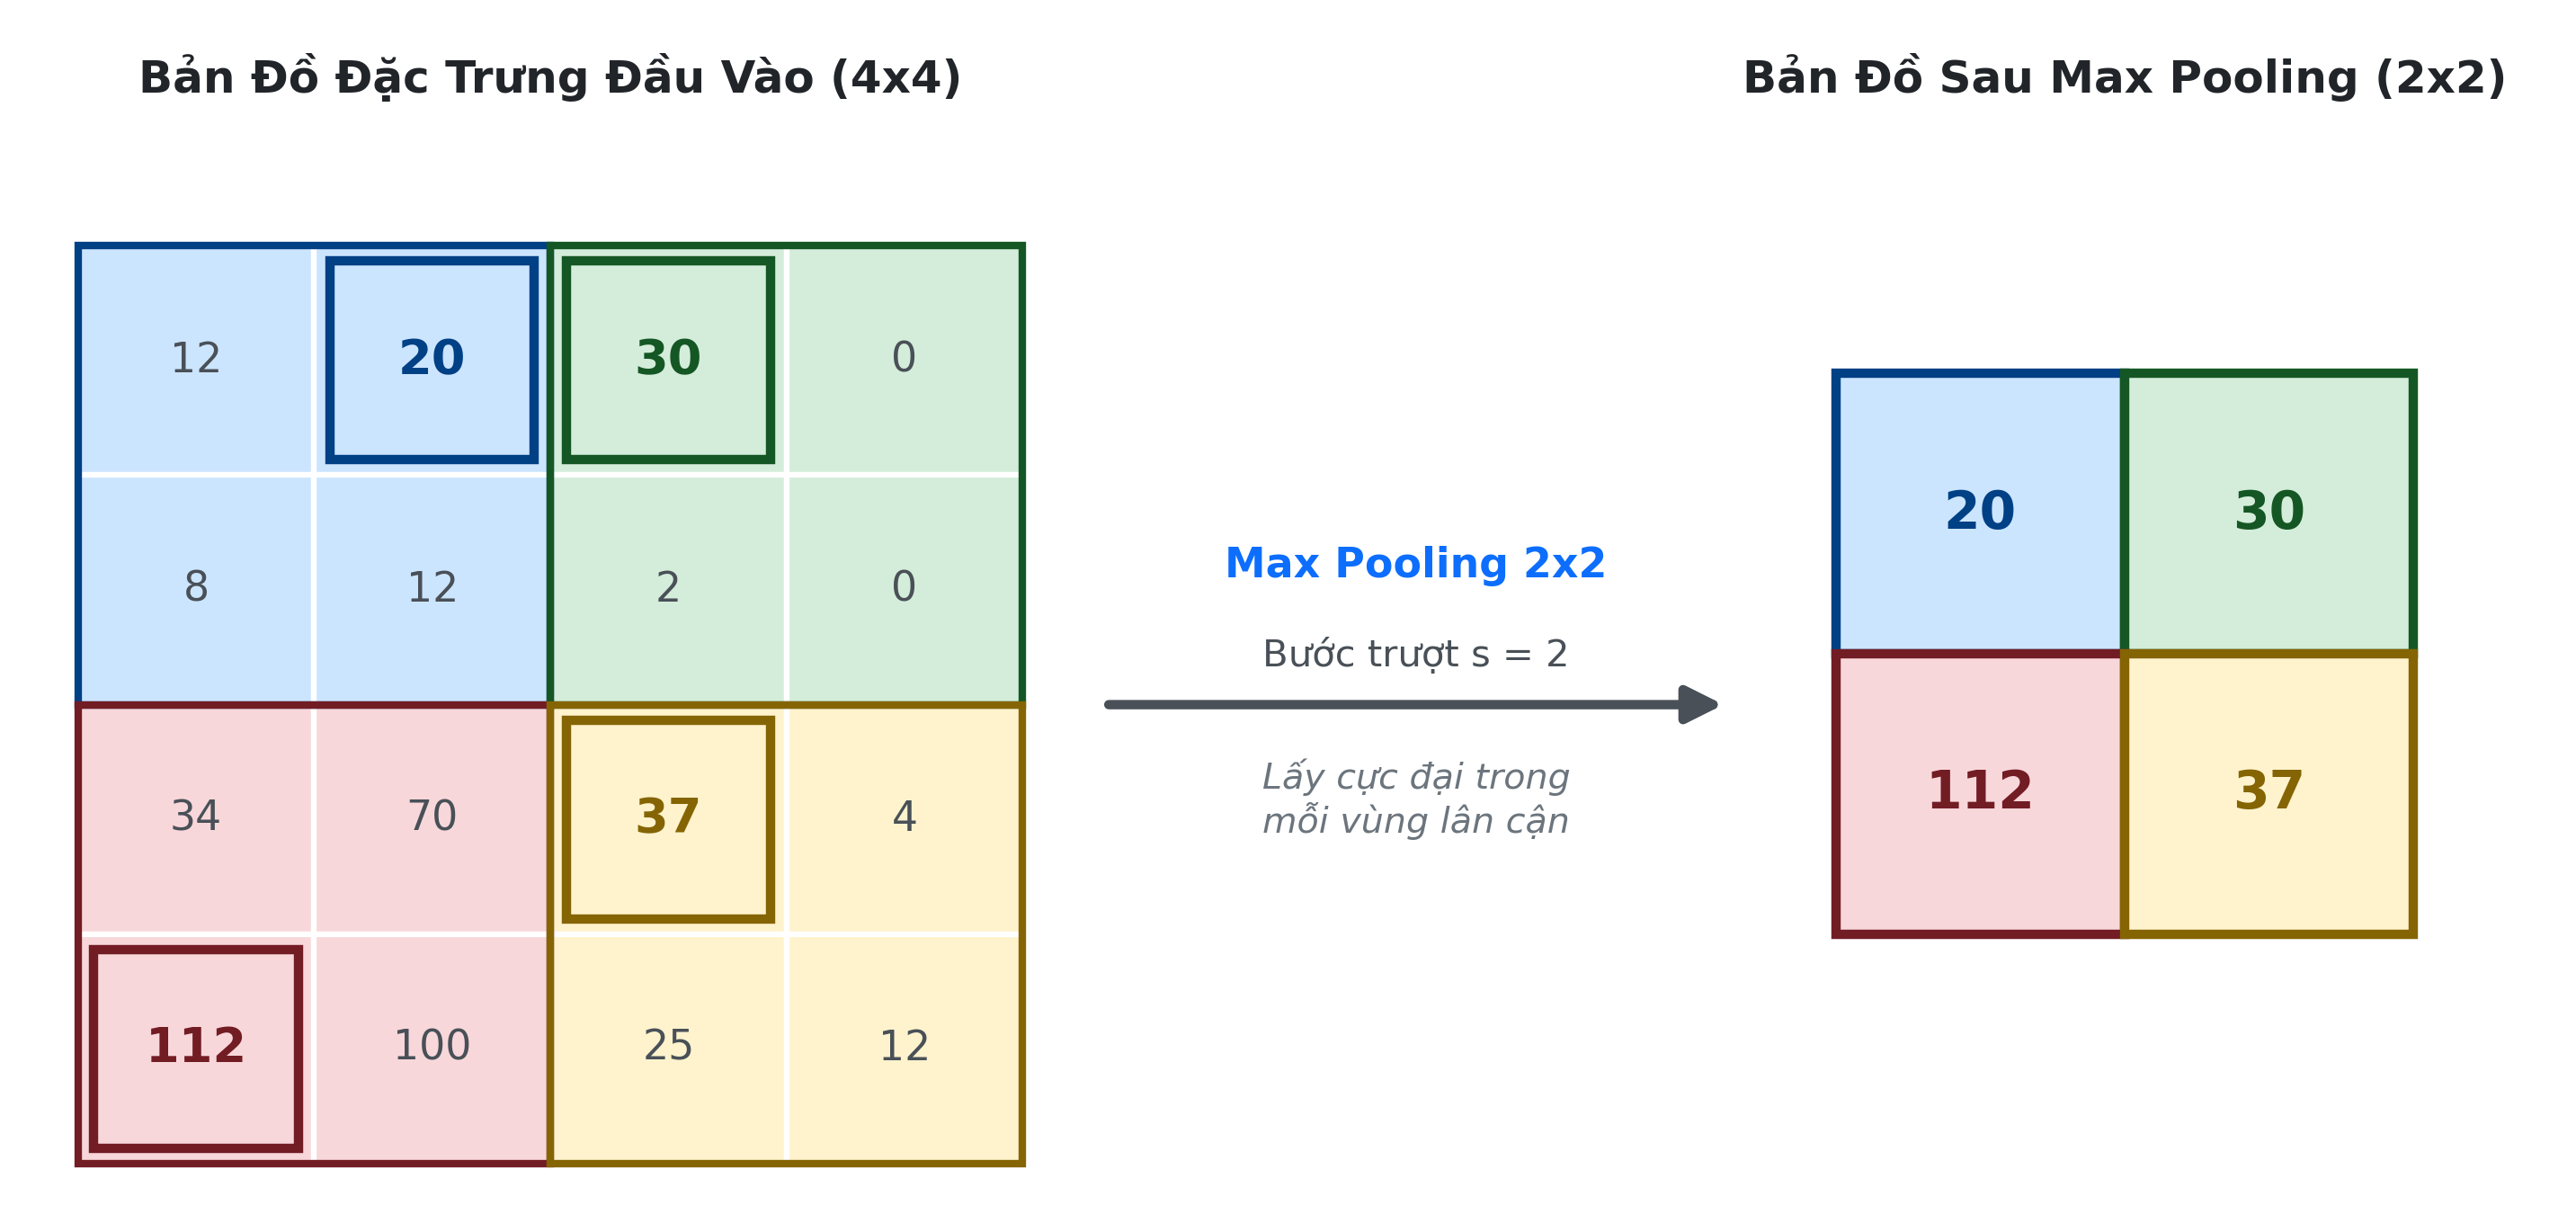
\includegraphics[width=0.90\textwidth]{images/fig09_max_pooling_detailed.png}
\caption{Cơ chế gom mẫu cực đại Max Pooling $2\times 2$ ($s=2$)}
\label{fig:max_pooling}
\end{figure}

\newpage

\subsection{Hàm Gom Cụm Trung Bình Toàn Cục (Global Average Pooling -- GAP)}
Một trong những bước tiến kiến trúc quan trọng nhất của học sâu (được đề xuất bởi Lin et al. trong bài báo Network-in-Network và hoàn thiện tại GoogLeNet, ResNet) là cơ chế \textbf{Gom cụm Trung bình Toàn cục (Global Average Pooling -- GAP)}.
\begin{equation}
\mathbf{v}(c) = \frac{1}{H \cdot W} \sum_{i=1}^H \sum_{j=1}^W A(i, j, c), \quad c = 1, \dots, C
\end{equation}
Thay vì làm phẳng một tensor 3D kích thước $(H \times W \times C)$ thành một vector khổng lồ rồi nối vào tầng Dense chứa hàng triệu tham số, GAP tính giá trị trung bình số học của toàn bộ $H \times W$ điểm ảnh trên mỗi kênh để thu được đúng một giá trị vô hướng cho mỗi kênh:
\begin{itemize}[leftmargin=2em]
    \item \textbf{Triệt tiêu bùng nổ tham số và chống quá khớp (Overfitting):} GAP hoàn toàn không chứa tham số học được (0 tham số). Nó thay thế trực tiếp các tầng Dense cồng kềnh, giảm từ 80\% đến 90\% tổng số tham số của toàn mạng.
    \item \textbf{Tính diễn giải hình học cao:} Mỗi kênh đặc trưng ở tầng tích chập cuối cùng đóng vai trò như một ``bản đồ độ tin cậy của danh mục'' (Category Confidence Map), phản ánh mức độ hiện diện của các thuộc tính tương ứng với lớp phân loại.
    \item \textbf{Mạng tích chập hoàn toàn (Fully Convolutional Network):} Mạng sử dụng GAP có khả năng tiếp nhận ảnh đầu vào với kích thước không gian tùy ý khi suy luận mà không bị bó hẹp bởi kích thước cố định như tầng Dense truyền thống.
\end{itemize}

\begin{figure}[H]
\centering
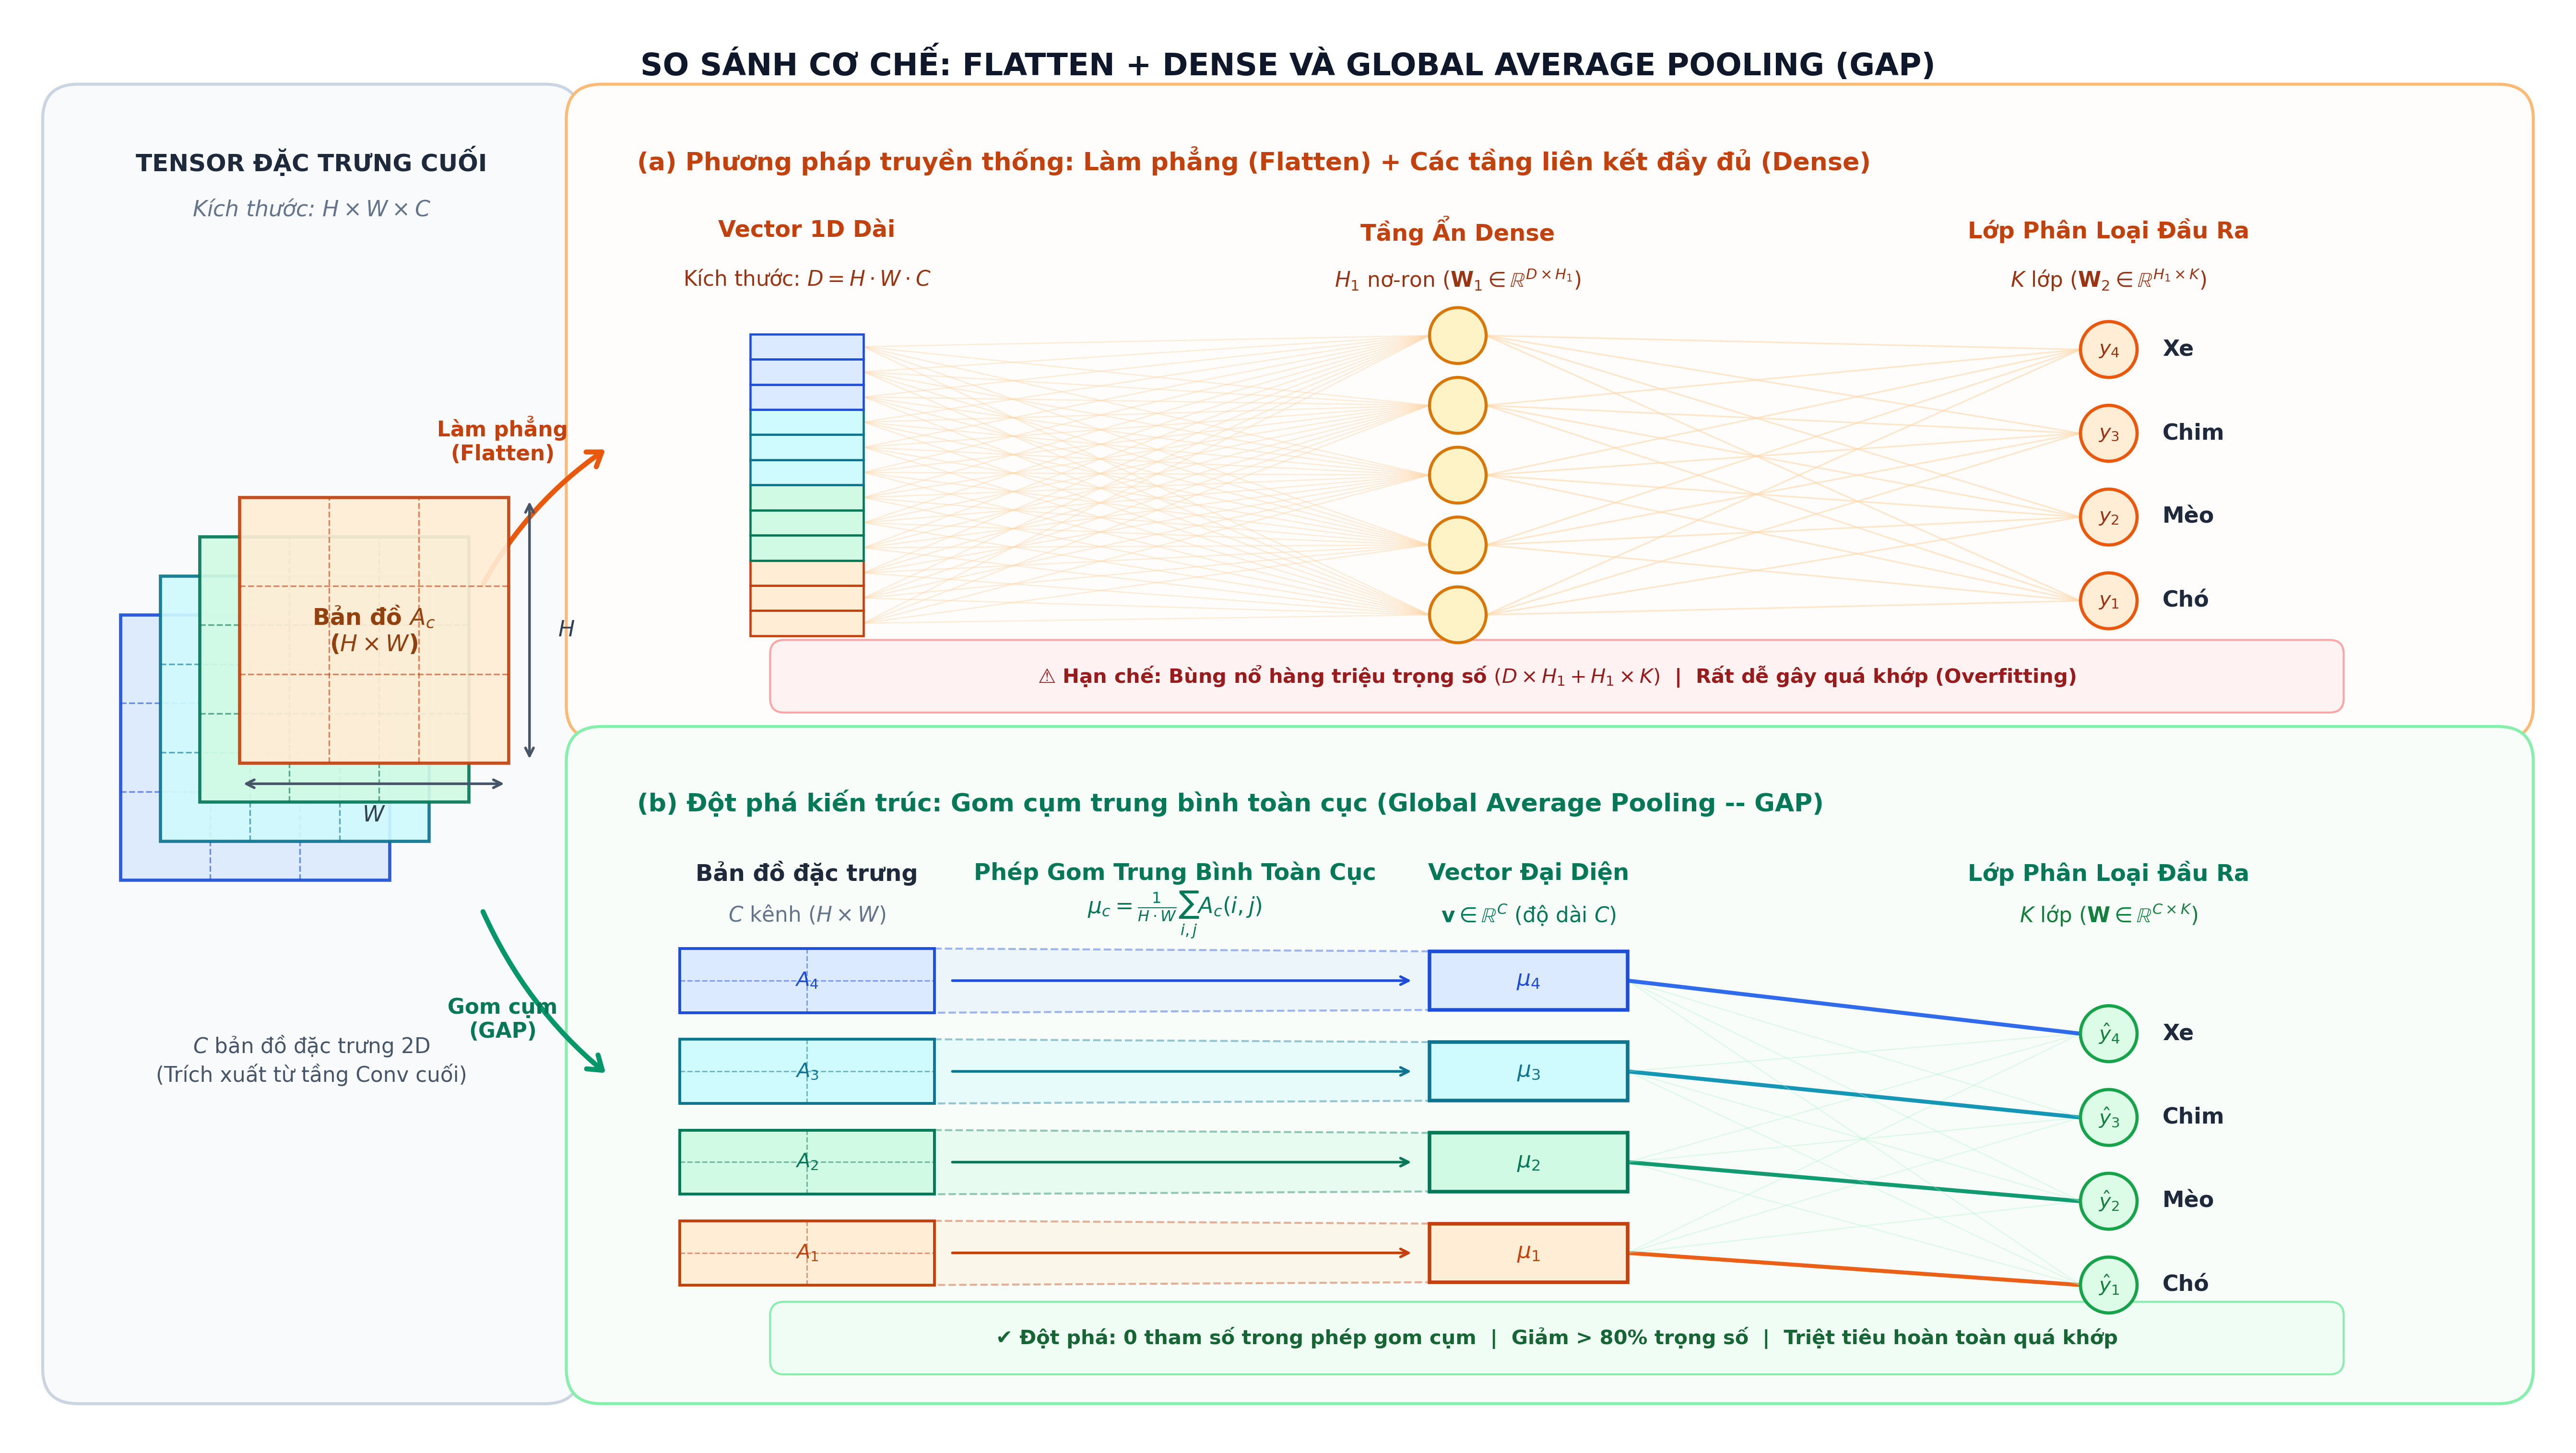
\includegraphics[width=0.92\textwidth]{images/fig10_gap_detailed.png}
\caption{Cơ chế gom cụm trung bình toàn cục (Global Average Pooling)}
\label{fig:gap}
\end{figure}

\newpage

\section{Mô Hình Toán Học Dạng Hàm Hợp (Composite Function) Của CNN}

\subsection{Bản Chất Toán Học Của Hàm Hợp Toàn Mạng}
Trong đại số giải tích, toàn bộ quy trình tính toán của một mạng nơ-ron tích chập $L$ tầng được mô hình hóa chính xác như một \textbf{phép hợp thành hàm toán học đa tầng có tham số} (Composite Function):
\begin{equation}
\hat{\mathbf{y}} = f(\mathbf{X}; \theta) = \left( f_L \circ f_{L-1} \circ \dots \circ f_3 \circ f_2 \circ f_1 \right)(\mathbf{X})
\label{eq:composite_function}
\end{equation}
trong đó mỗi hàm thành phần $f_l$ là một ánh xạ xác định biến đổi giữa các không gian tensor:
\begin{equation}
f_l: \mathcal{T}_{l-1} \longrightarrow \mathcal{T}_l, \quad \mathbf{Z}_l = f_l(\mathbf{Z}_{l-1}; \mathbf{W}^{[l]}, \mathbf{b}^{[l]})
\end{equation}
và tập tham số toàn cục của mạng là hợp các tham số học được tại từng tầng ánh xạ:
\begin{equation}
\theta = \bigcup_{l=1}^L \{ \mathbf{W}^{[l]}, \mathbf{b}^{[l]} \}
\end{equation}

\begin{figure}[H]
\centering
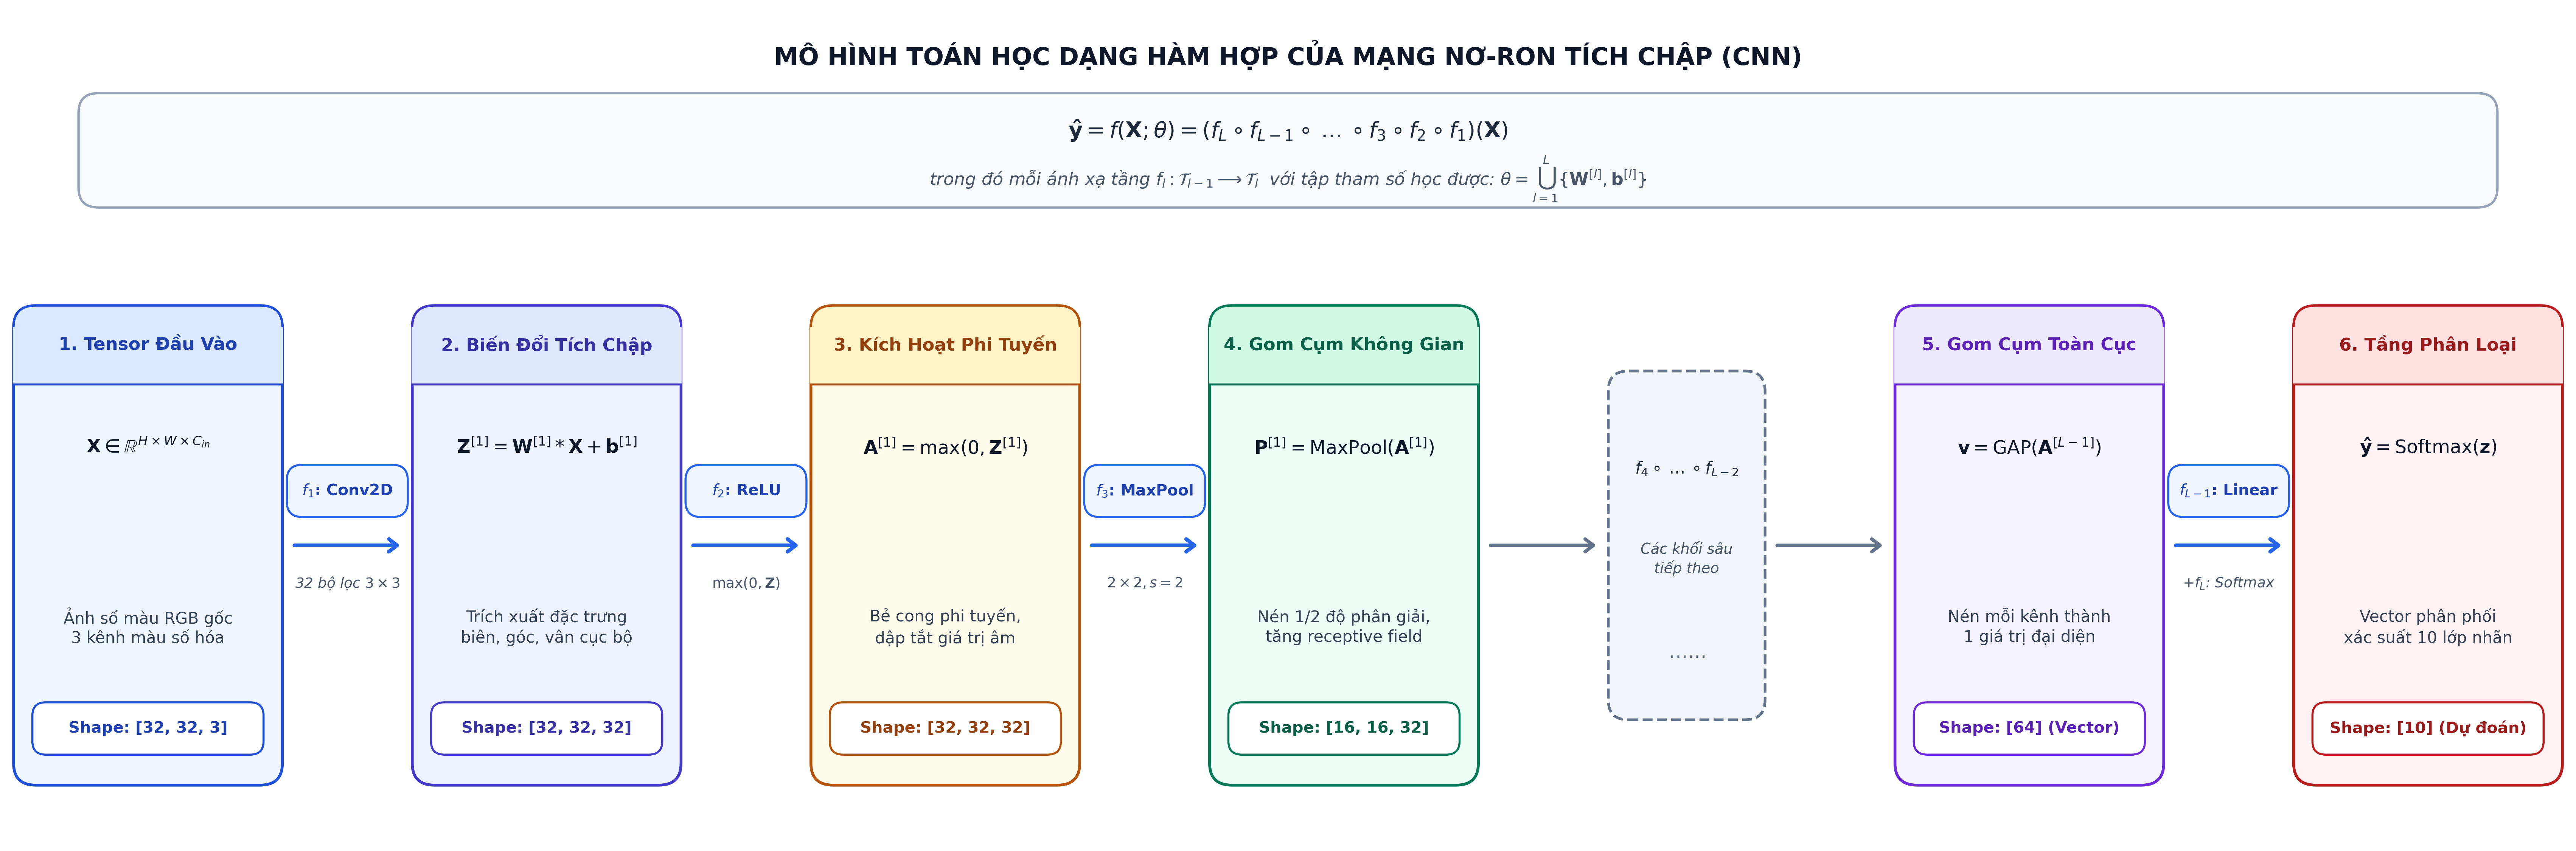
\includegraphics[width=0.95\textwidth]{images/fig01_composite_function_flow.png}
\caption{Sơ đồ dòng chảy ánh xạ tensor trong mạng CNN}
\label{fig:composite_flow}
\end{figure}

\subsection{Phân Tích Chi Tiết Dòng Chảy Kích Thước Tensor (Tensor Shape Flow)}
Bảng \ref{tab:tensor_shape_flow} giải phẫu chính xác sự chuyển dịch không gian vector và số lượng tham số qua từng hàm thành phần của một mạng CNN cơ bản nhận ảnh đầu vào $32 \times 32 \times 3$:

\begin{table}[H]
\centering
\footnotesize
\caption{Giải phẫu chi tiết luồng ánh xạ không gian và tham số trong hàm hợp CNN}
\label{tab:tensor_shape_flow}
\begin{tabularx}{\textwidth}{c >{\raggedright\arraybackslash}X c c r}
\toprule
\textbf{Bước} & \textbf{Hàm Ánh Xạ $f_l$} & \textbf{Không Gian Vào} & \textbf{Không Gian Ra} & \textbf{Tham Số Học Được} \\
\midrule
$f_1$ & $\mathbf{Conv2D}$ (Kernel $3\times 3$, P=1) & $\mathbb{R}^{32 \times 32 \times 3}$ & $\mathbb{R}^{32 \times 32 \times 32}$ & $(3\times 3\times 3 + 1)\times 32 = 896$ \\
$f_2$ & $\mathbf{ReLU}$ (Kích hoạt phi tuyến) & $\mathbb{R}^{32 \times 32 \times 32}$ & $\mathbb{R}^{32 \times 32 \times 32}$ & $0$ \\
$f_3$ & $\mathbf{MaxPool2D}$ (Cửa sổ $2\times 2$, s=2) & $\mathbb{R}^{32 \times 32 \times 32}$ & $\mathbb{R}^{16 \times 16 \times 32}$ & $0$ \\
$f_4$ & $\mathbf{Conv2D}$ (Kernel $3\times 3$, P=1) & $\mathbb{R}^{16 \times 16 \times 32}$ & $\mathbb{R}^{16 \times 16 \times 64}$ & $(3\times 3\times 32 + 1)\times 64 = 18,496$ \\
$f_5$ & $\mathbf{ReLU}$ (Kích hoạt phi tuyến) & $\mathbb{R}^{16 \times 16 \times 64}$ & $\mathbb{R}^{16 \times 16 \times 64}$ & $0$ \\
$f_6$ & $\mathbf{MaxPool2D}$ (Cửa sổ $2\times 2$, s=2) & $\mathbb{R}^{16 \times 16 \times 64}$ & $\mathbb{R}^{8 \times 8 \times 64}$ & $0$ \\
$f_7$ & $\mathbf{GAP}$ (Nén không gian toàn cục) & $\mathbb{R}^{8 \times 8 \times 64}$ & $\mathbb{R}^{64}$ & $0$ \\
$f_8$ & $\mathbf{Linear}$ (Chiếu sang 10 lớp nhãn) & $\mathbb{R}^{64}$ & $\mathbb{R}^{10}$ & $(64 + 1)\times 10 = 650$ \\
$f_9$ & $\mathbf{Softmax}$ (Chuẩn hóa xác suất) & $\mathbb{R}^{10}$ & $[0, 1]^{10}$ & $0$ \\
\midrule
\multicolumn{4}{l}{\textbf{Tổng số lượng tham số học được của toàn bộ Hàm Hợp:}} & \textbf{20,042} \\
\bottomrule
\end{tabularx}
\end{table}

\newpage

\section{Hiện Thực Hóa Mã Nguồn Toán Học \& Kiểm Chứng Thực Nghiệm}

Nhằm kiểm chứng tính chính xác của các mô hình giải tích đã thiết lập, phần này trình bày mã nguồn hiện thực hóa chi tiết các toán tử cốt lõi của mạng nơ-ron tích chập và mô hình hàm hợp bằng ngôn ngữ Python (sử dụng thư viện tính toán số trị NumPy):

\subsection{Cài Đặt Hàm Tích Chập 2D Đa Kênh Thuần Toán Học}
Listing \ref{lst:conv2d_explicit} thể hiện tường minh $100\%$ các vòng lặp tính toán cửa sổ trượt, áp dụng đệm viền và tích vô hướng Frobenius:

\begin{lstlisting}[language=Python, caption={Cài đặt hàm tích chập 2D đa kênh thuần giải tích bằng NumPy}, label={lst:conv2d_explicit}]
def conv2d_forward_explicit(X, W, b, stride=1, padding=0):
    H_in, W_in, C_in = X.shape
    K_h, K_w, C_in_w, C_out = W.shape
    assert C_in == C_in_w, "So kenh dau vao phai khop so kenh cua bo loc!"
    
    # 1. Ap dung dem vien Zero-Padding
    if padding > 0:
        X_padded = np.pad(X, ((padding, padding), (padding, padding), (0, 0)), 
                          mode="constant", constant_values=0)
    else:
        X_padded = X
        
    # 2. Tinh toan kich thuoc khong gian dau ra
    H_out = int(np.floor((H_in + 2 * padding - K_h) / stride)) + 1
    W_out = int(np.floor((W_in + 2 * padding - K_w) / stride)) + 1
    Z = np.zeros((H_out, W_out, C_out), dtype=np.float32)
    
    # 3. Quet cua so truot tren tung kenh va cong don chieu sau
    for m in range(C_out):
        for i in range(H_out):
            for j in range(W_out):
                h_start = i * stride
                h_end = h_start + K_h
                w_start = j * stride
                w_end = w_start + K_w
                X_slice = X_padded[h_start:h_end, w_start:w_end, :]
                Z[i, j, m] = np.sum(X_slice * W[:, :, :, m]) + b[m]
    return Z
\end{lstlisting}

\subsection{Cài Đặt Lớp Kiến Trúc Hàm Hợp Bằng PyTorch}
Listing \ref{lst:composite_cnn} định nghĩa lớp \texttt{ExplicitCompositeCNN}, trong đó mỗi hàm thành phần $f_1, \dots, f_9$ được phân tách thành từng thuộc tính và tính toán tuần tự:

\begin{lstlisting}[language=Python, caption={Cài đặt lớp ExplicitCompositeCNN thể hiện tường minh mô hình hàm hợp}, label={lst:composite_cnn}]
class ExplicitCompositeCNN(nn.Module):
    def __init__(self, num_classes=10):
        super().__init__()
        # Khoi dac trung 1: f_1 (Conv) -> f_2 (ReLU) -> f_3 (Pool)
        self.f1_conv1 = nn.Conv2d(in_channels=3, out_channels=32, kernel_size=3, padding=1)
        self.f2_relu1 = nn.ReLU()
        self.f3_pool1 = nn.MaxPool2d(kernel_size=2, stride=2)
        
        # Khoi dac trung 2: f_4 (Conv) -> f_5 (ReLU) -> f_6 (Pool)
        self.f4_conv2 = nn.Conv2d(in_channels=32, out_channels=64, kernel_size=3, padding=1)
        self.f5_relu2 = nn.ReLU()
        self.f6_pool2 = nn.MaxPool2d(kernel_size=2, stride=2)
        
        # f_7: Global Average Pooling (GAP)
        self.f7_gap = nn.AdaptiveAvgPool2d((1, 1))
        
        # f_8: Phep bien doi Affine
        self.f8_linear = nn.Linear(in_features=64, out_features=num_classes)
        
        # f_9: Chuan hoa xac suat Softmax
        self.f9_softmax = nn.Softmax(dim=-1)

    def forward(self, x):
        # Lan truyen tien: f = (f_9 o f_8 o ... o f_1)(x)
        x = self.f1_conv1(x)
        x = self.f2_relu1(x)
        x = self.f3_pool1(x)
        x = self.f4_conv2(x)
        x = self.f5_relu2(x)
        x = self.f6_pool2(x)
        v = torch.flatten(self.f7_gap(x), 1)
        return self.f9_softmax(self.f8_linear(v))
\end{lstlisting}

\subsection{Trực Quan Hóa Bản Đồ Đặc Trưng Trung Gian (Feature Maps)}
Khi đưa ảnh qua hàm hợp, các bản đồ đặc trưng ở từng giai đoạn thể hiện rõ ràng tính chất phân cấp thứ bậc của thị giác:
\begin{itemize}[leftmargin=2em]
    \item \textbf{Tầng đầu $f_2$:} Kích hoạt mạnh tại các đường biên, cạnh viền sắc nét, tương ứng với chức năng của các tế bào đơn giản (Simple Cells).
    \item \textbf{Tầng sâu $f_5$:} Bản đồ có kích thước không gian nhỏ hơn ($16 \times 16$) nhưng mức độ biểu cảm phong phú hơn, phản ánh các cấu trúc họa tiết và hoa văn trừu tượng có ý nghĩa phân loại cao.
\end{itemize}

\begin{figure}[H]
\centering
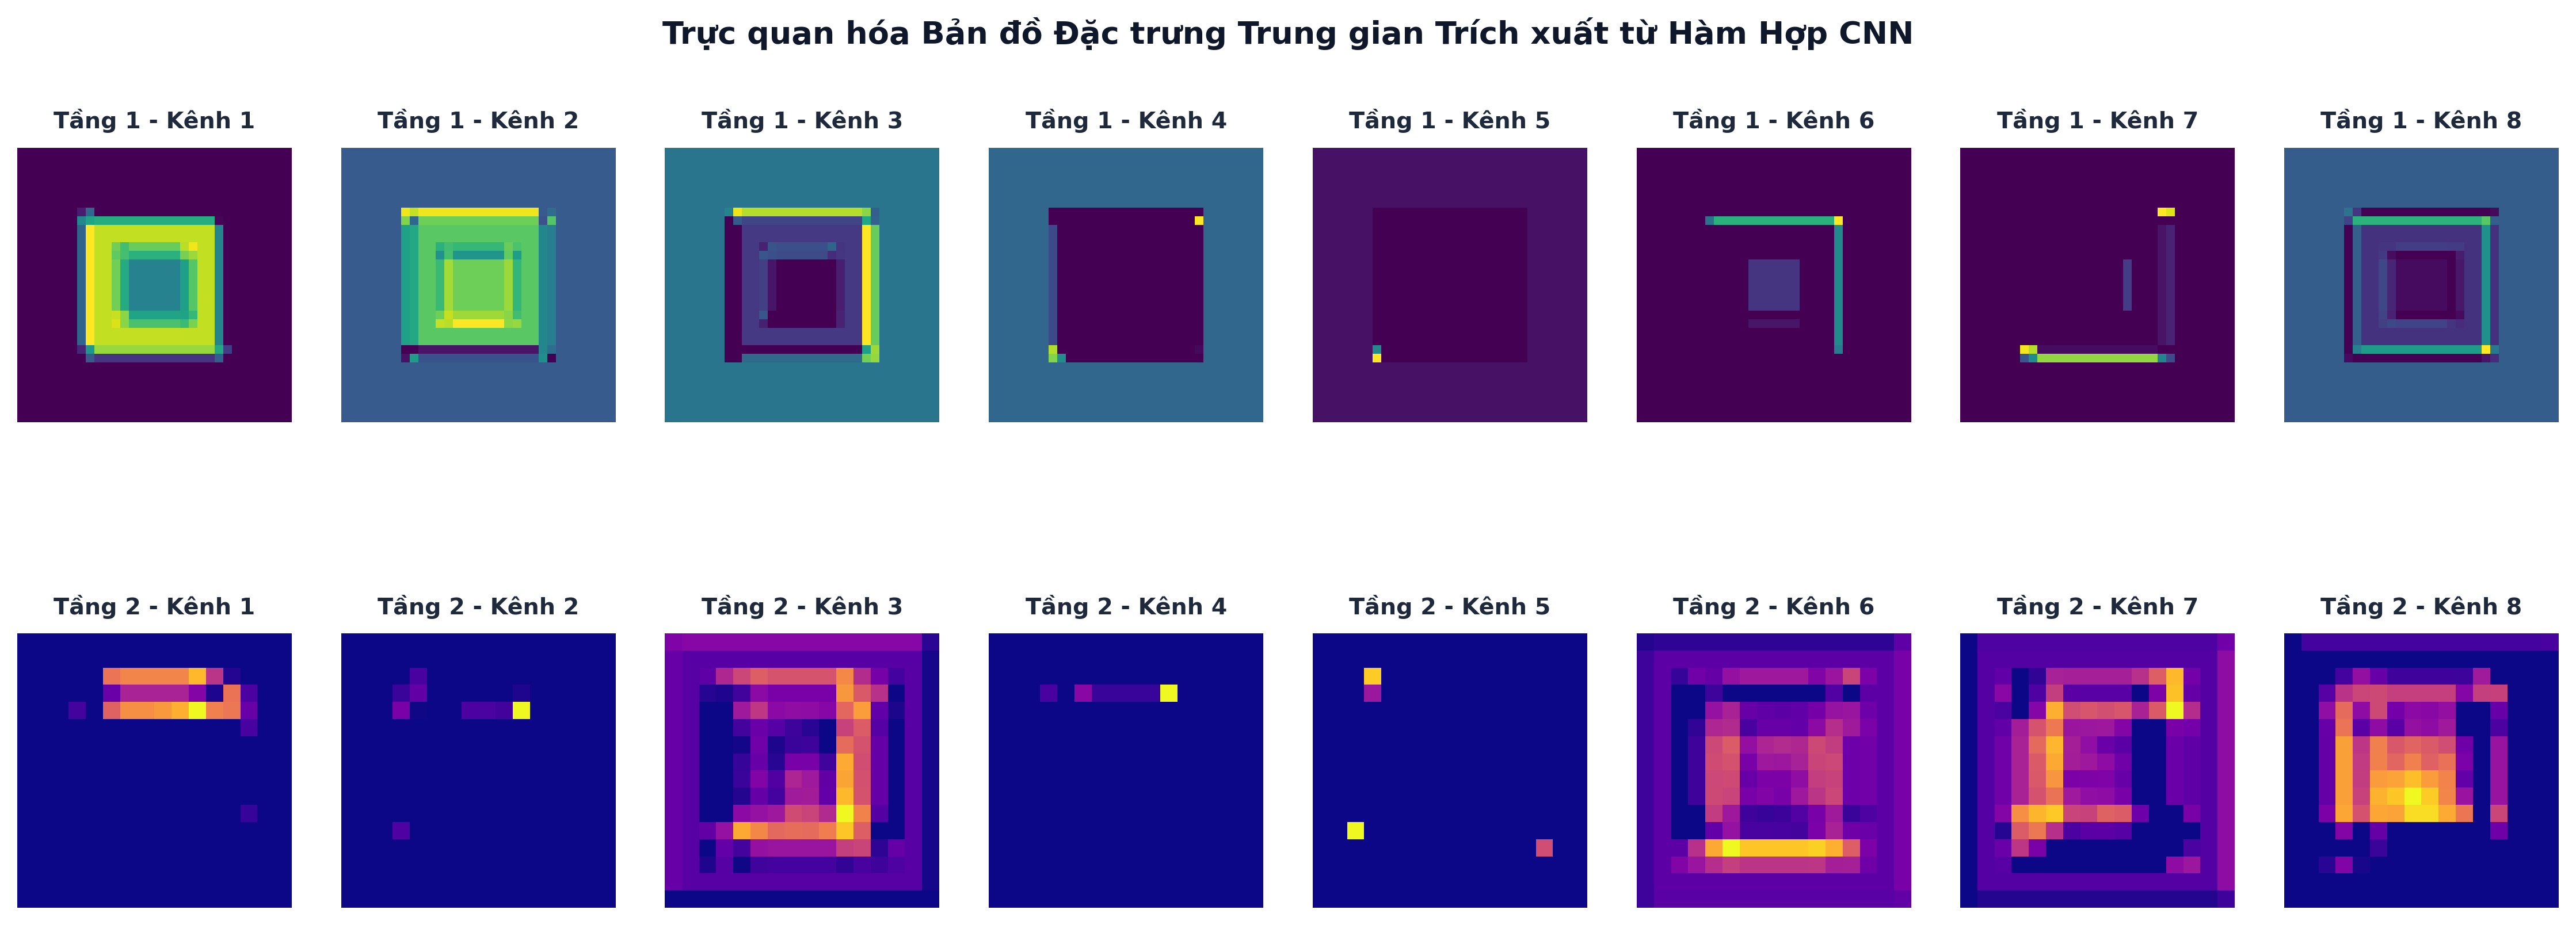
\includegraphics[width=0.95\textwidth]{images/fig04_intermediate_feature_maps.png}
\caption{Bản đồ đặc trưng trích xuất từ các tầng ẩn của CNN}
\label{fig:feature_maps}
\end{figure}

\section{Tóm Tắt Chương 1}
Qua phân tích giải tích và hiện thực hóa mã nguồn trong Chương 1:
\begin{enumerate}[leftmargin=1.5em]
    \item Đã làm rõ nguồn gốc sinh học và chứng minh bản chất của mạng CNN là một \textbf{hàm hợp đa tầng} $f = (f_L \circ \dots \circ f_1)$ bảo toàn cấu trúc tô-pô không gian 2D, giải quyết triệt để 3 hạn chế chí mạng của mạng MLP truyền thống.
    \item Đã làm sáng tỏ tường minh cơ chế toán học và hình học của từng toán tử thành phần: tính toán số học tích chập từng bước, tích chập 3D đa kênh gom theo chiều sâu, đệm viền Zero-Padding, bước trượt Stride, độ giãn nở Dilation, nguyên lý mở rộng trường tiếp nhận hiệu dụng với bộ lọc $3\times 3$, hàm kích hoạt phi tuyến ReLU triệt tiêu bão hòa gradient, và hai cơ chế gom cụm (Max Pooling cục bộ và GAP nén toàn cục).
    \item Toàn bộ các thuật toán và mô hình hàm hợp toán học đã được kiểm chứng thực nghiệm độc lập thông qua bộ mã nguồn kiểm thử số trị, xác lập cơ sở lý thuyết và phương pháp luận vững chắc để triển khai sang \textbf{Chương 2: Các Mô Hình Tiến Hóa Kiến Trúc Kinh Điển (VGG, ResNet, MobileNet)}.
\end{enumerate}

\chapter{Các Mô Hình Tiến Hóa Kiến Trúc Kinh Điển (VGG, ResNet, MobileNet)}

\section{Động Lực Phát Triển \& Bức Tranh Tổng Thể Tiến Hóa Kiến Trúc}

\subsection{Bối Cảnh Lịch Sử: Từ Mạng Nguyên Khối Đến Thiết Kế Hướng Khối}
Sự phát triển của Mạng Nơ-ron Tích chập (CNN) trong hơn hai thập kỷ qua là minh chứng điển hình cho sự tiến hóa của các hệ hình thiết kế kiến trúc học sâu. Quá trình này có thể chia thành hai giai đoạn bản lề:
\begin{itemize}[leftmargin=2em]
    \item \textbf{Giai đoạn khởi nguyên và thiết kế nguyên khối (1998 -- 2012):} Mở đầu với LeNet-5 (LeCun et al., 1998) giải quyết bài toán nhận diện chữ số viết tay trên bộ dữ liệu MNIST. Đến năm 2012, AlexNet (Krizhevsky et al.) tạo nên cú hích lịch sử tại cuộc thi ImageNet Large Scale Visual Recognition Challenge (ILSVRC) khi giảm tỉ lệ lỗi phân loại Top-5 từ 26\% xuống còn 15.3\%. Tuy nhiên, đặc điểm chung của các mạng trong giai đoạn này là cấu trúc mang tính \textbf{nguyên khối (Monolithic)}: các siêu tham số (kích thước kernel, bước trượt stride, số kênh) được bố trí thủ công, sử dụng các bộ lọc không gian rất lớn ($11 \times 11$, $5 \times 5$), và phần lớn tham số tập trung tại các tầng kết nối đầy đủ (Fully Connected -- FC).
    \item \textbf{Kỷ nguyên chuẩn hóa hướng khối (Modular Block-based Design, 2014 -- nay):} Kể từ sau năm 2014, cộng đồng nghiên cứu chuyển dịch hoàn toàn sang phương pháp luận module hóa. Thay vì thiết kế từng tầng riêng rẽ, mạng nơ-ron được cấu thành từ việc lặp lại các \textbf{khối kiến trúc vi mô chuẩn hóa (Micro-architectural Blocks)}. Sự chuyển dịch này không chỉ giúp đơn giản hóa việc tối ưu hóa mà còn mở đường cho việc xây dựng các mạng nơ-ron cực sâu và cực kỳ hiệu quả về mặt tài nguyên tính toán.
\end{itemize}

\subsection{Ba Thách Thức Cốt Lõi Thúc Đẩy Đột Phá Kiến Trúc}
Sự tiến hóa từ các mạng nguyên khối sang các kiến trúc hiện đại được thúc đẩy bởi ba bài toán kỹ thuật nền tảng:

\begin{enumerate}[leftmargin=2em]
    \item \textbf{Thách thức bùng nổ tham số do bộ lọc lớn và tầng Fully Connected:}
    Trong các mạng cổ điển như AlexNet (Hình \ref{fig:alexnet_monolithic}A), tầng tích chập đầu tiên sử dụng bộ lọc không gian rất lớn ($11 \times 11$), đòi hỏi $11 \times 11 \times 3 \times 96 = 34{,}848$ trọng số. Tuy nhiên, điểm nghẽn nghiêm trọng nhất của kiến trúc nguyên khối nằm ở sự chuyển giao từ giai đoạn trích xuất đặc trưng tích chập sang giai đoạn phân loại:
    \begin{itemize}[leftmargin=1.5em]
        \item \textit{Điểm nghẽn bùng nổ tham số tại tầng Flatten và FC-6:} Sau 5 tầng Conv-MaxPool, tensor bản đồ đặc trưng cuối cùng có kích thước $6 \times 6 \times 256$ ($9{,}216$ giá trị). Để đưa vào bộ phân loại dày đặc, mạng buộc phải thực hiện phép trải phẳng (Flatten) thành vector $1\mathrm{D}$ kích thước $9{,}216$. Khi kết nối toàn phần vào tầng $\text{FC-6}$ gồm $4{,}096$ nơ-ron, ma trận trọng số tương ứng có kích thước $\mathbf{W}_{\text{FC6}} \in \mathbb{R}^{9{,}216 \times 4{,}096}$, tiêu tốn tới $9{,}216 \times 4{,}096 = 37{,}748{,}736$ trọng số cùng $4{,}096$ hệ số chệch, tổng cộng hơn $37.75$ triệu tham số. Chỉ riêng tầng này đã chiếm tới $60.55\%$ tổng số tham số của toàn bộ mô hình ($62.37$ triệu tham số). Nếu tính cả 3 tầng Fully Connected ($\text{FC-6}$, $\text{FC-7}$, $\text{FC-8}$), tổng lượng tham số lên tới $58.63$ triệu, chiếm áp đảo $93.99\%$ dung lượng lưu trữ của toàn mạng (tương đương $>234\text{ MB}$ ở định dạng float32).
        
        \item \textit{Nghịch lý đối nghịch giữa Tham số và Khối lượng tính toán (FLOPs):} Phân tích định lượng tại Hình \ref{fig:alexnet_monolithic}B chỉ ra một sự mất cân đối cực đoan: $5$ tầng tích chập (Conv Backbone) đảm nhận tới $95.0\%$ toàn bộ khối lượng tính toán số học dấu phẩy động ($\approx 0.68\text{ GFLOPs}$ trên tổng số $0.72\text{ GFLOPs}$), nhưng chỉ chứa vỏn vẹn $6.01\%$ tham số ($3.74$ triệu tham số). Ngược lại, $3$ tầng Fully Connected tiêu tốn tới gần $94\%$ tham số nhưng chỉ đóng góp chưa đầy $5.0\%$ khối lượng tính toán.
        
        \item \textit{Hệ quả quá khớp và sự bắt buộc sử dụng Dropout cực đoan:} Sự tập trung tới gần $60$ triệu tham số tự do tại phần đuôi mạng làm tăng đột biến dung lượng mô hình (model capacity), khiến mạng rất dễ ghi nhớ vẹt dữ liệu huấn luyện (Overfitting). Để kiểm soát nguy cơ này, Krizhevsky et al. bắt buộc phải áp dụng kỹ thuật Dropout với tỷ lệ ngắt bỏ nơ-ron cực cao ($p = 0.5$) tại hai tầng $\text{FC-6}$ và $\text{FC-7}$, ép các nơ-ron phải học các biểu diễn phân tán và ngăn chặn hiện tượng đồng thích ứng (co-adaptation).
        
        \item \textit{Động lực chuyển dịch sang Khối vi mô và Global Average Pooling (GAP):} Điểm nghẽn tham số của AlexNet đã trực tiếp thúc đẩy hai cải tiến kiến trúc mang tính lịch sử: (1) Chuẩn hóa các khối tích chập vi mô $3 \times 3$ trong VGG để tiết kiệm tham số bộ lọc; và (2) Thay thế hoàn toàn các tầng Fully Connected cồng kềnh bằng tầng Gom cụm trung bình toàn cục (Global Average Pooling -- GAP) khởi xướng từ Network-In-Network (Lin et al., 2013) và sau đó trở thành chuẩn mực trong ResNet, MobileNet. Kỹ thuật GAP tính giá trị trung bình trên từng kênh không gian để chuyển đổi trực tiếp tensor $H \times W \times C$ thành vector $1 \times C$, giảm số tham số chuyển tiếp về $0$ và bảo toàn tối đa ý nghĩa không gian của các bản đồ đặc trưng.
    \end{itemize}

\begin{figure}[H]
\centering
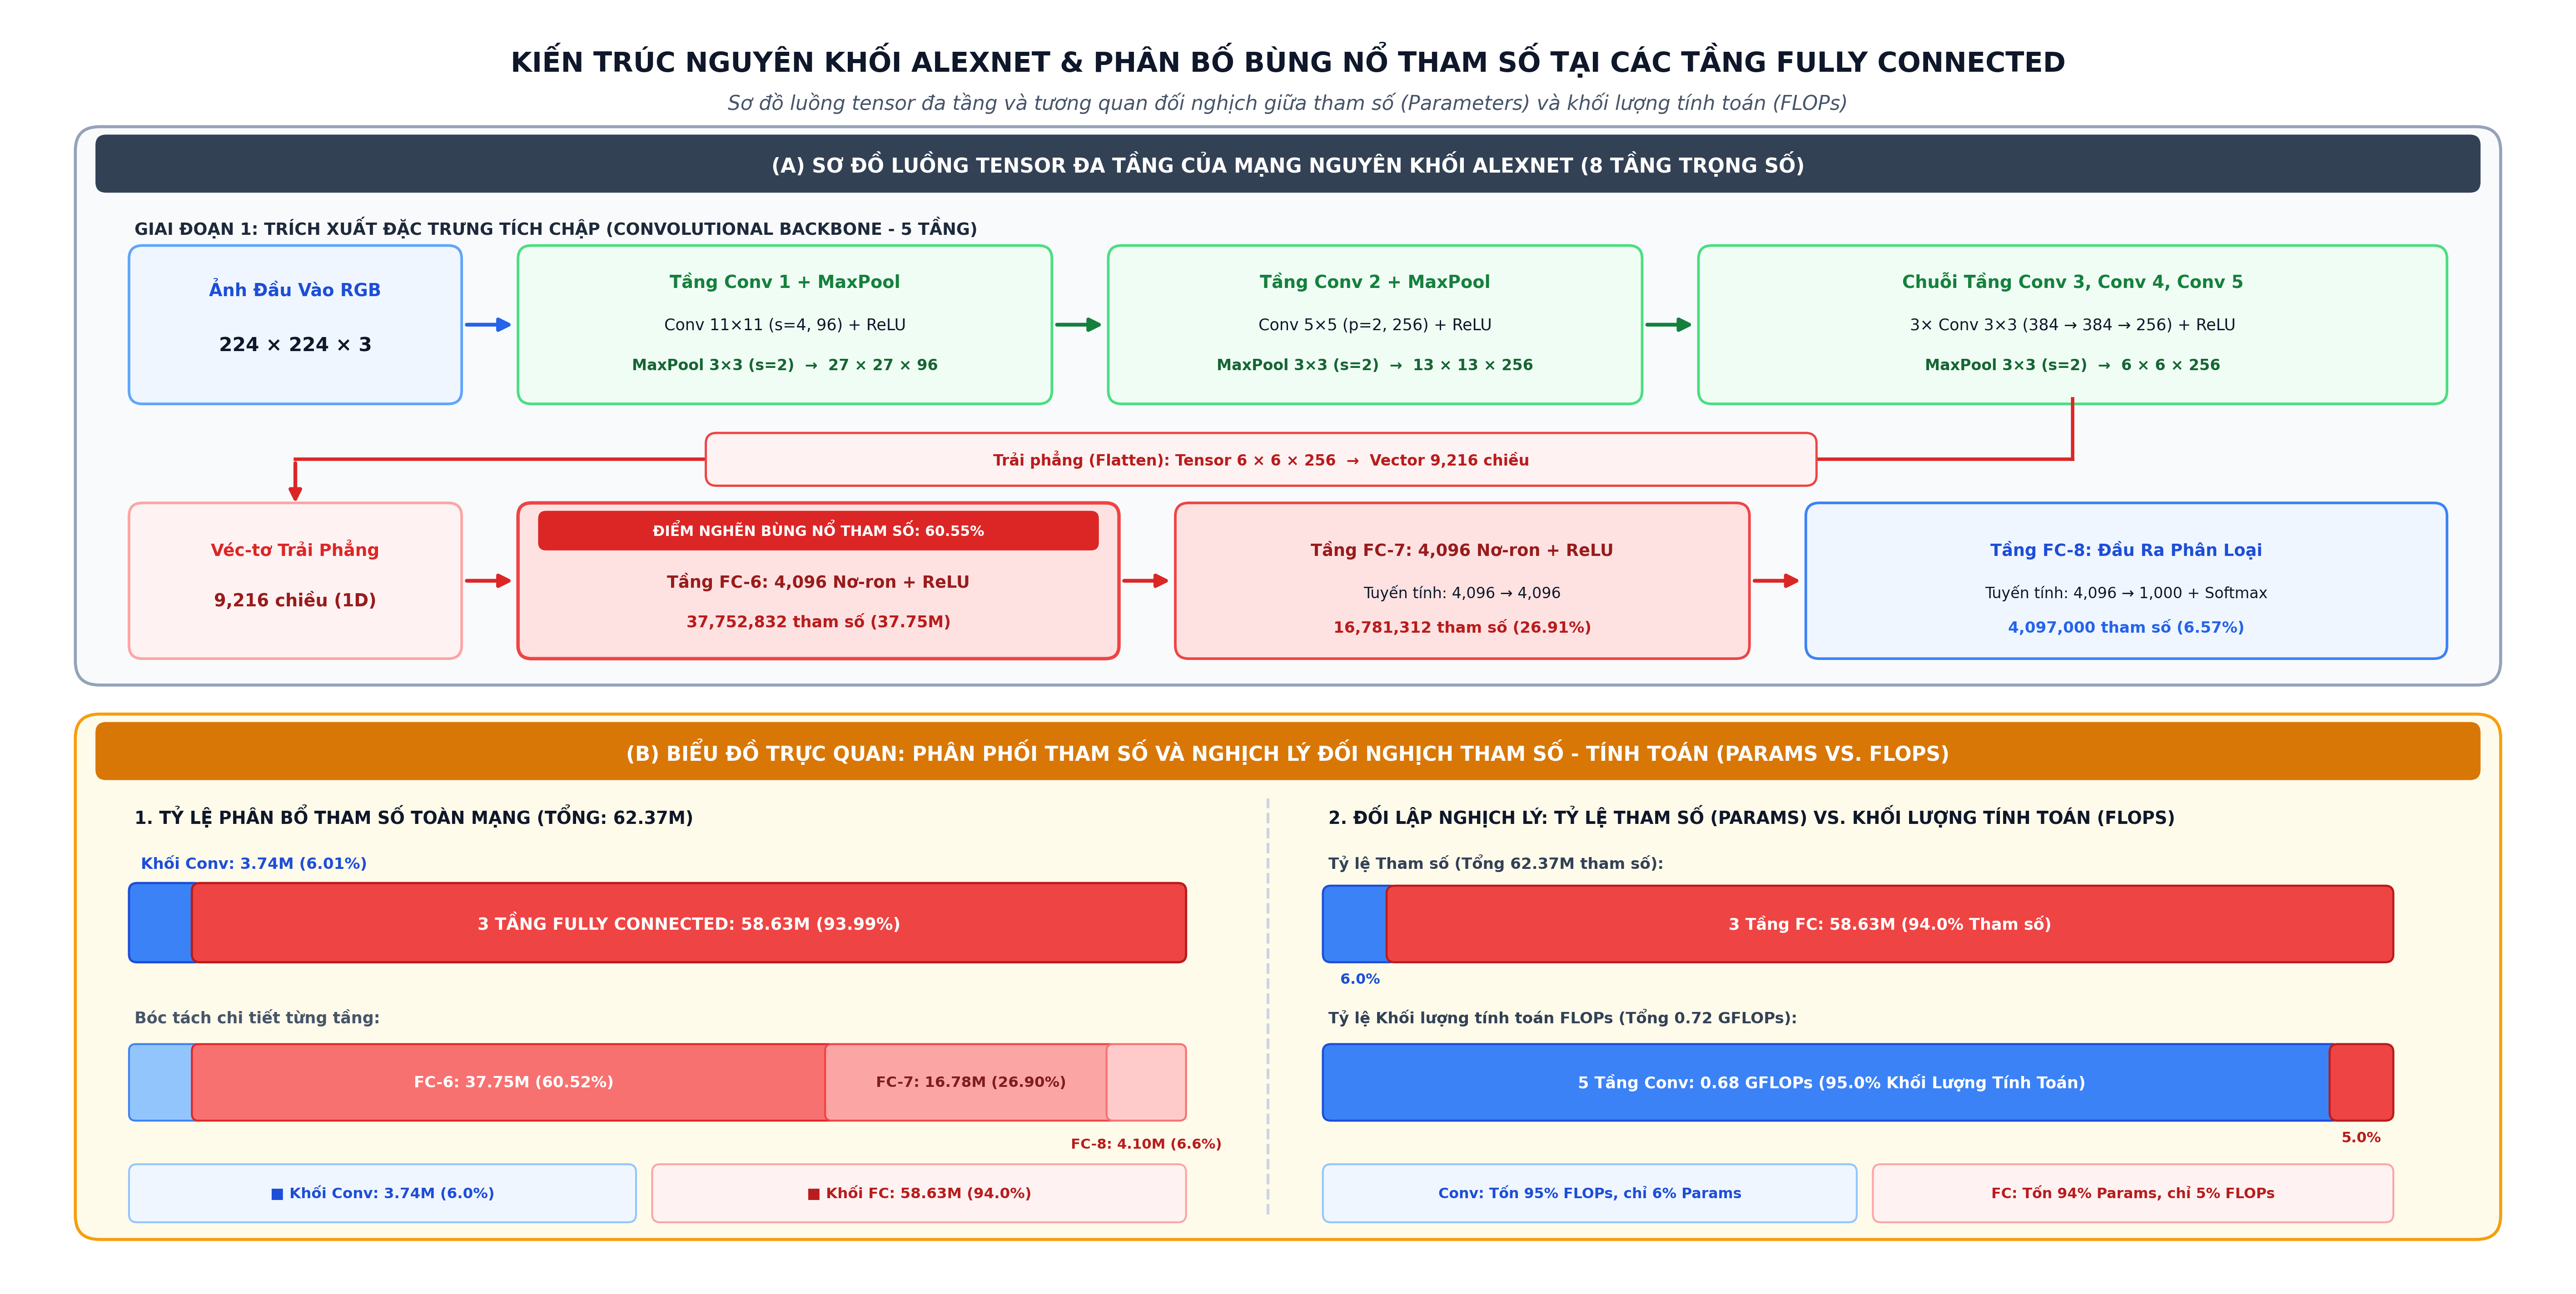
\includegraphics[width=0.96\textwidth]{images/fig201_alexnet_monolithic.png}
\caption{Kiến trúc nguyên khối AlexNet và phân bố tham số bùng nổ tại các tầng Fully Connected.}
\label{fig:alexnet_monolithic}
\end{figure}

    \item \textbf{Hiện tượng suy biến mạng sâu (Degradation Problem) \& Triệt tiêu Gradient:}
    Theo trực giác lý thuyết, khi tăng độ sâu mạng ($L \to \infty$), không gian hàm biểu diễn của mạng phải mở rộng, do đó một mạng sâu hơn ít nhất phải đạt được độ chính xác huấn luyện không kém hơn mạng nông (vì các tầng bổ sung có thể học ánh xạ đồng nhất $\mathbf{x} \mapsto \mathbf{x}$). Tuy nhiên, thực nghiệm trên các mạng thuần tích chập (Plain CNN) cho thấy: khi độ sâu vượt quá 20 tầng, cả độ chính xác trên tập kiểm tra lẫn tập huấn luyện đều bị suy thoái nghiêm trọng (Degradation). Vấn đề này bắt nguồn từ hiện tượng suy biến đạo hàm khi lan truyền ngược qua chuỗi tích ma trận dài:
    \begin{equation}
        \frac{\partial \mathcal{L}}{\partial \mathbf{x}_l} = \frac{\partial \mathcal{L}}{\partial \mathbf{x}_L} \prod_{k=l}^{L-1} \mathbf{W}_{k+1}^T \text{diag}\big(\sigma'(\mathbf{z}_k)\big)
    \end{equation}
    Khi các giá trị riêng hoặc chuẩn phổ của các ma trận trọng số $\mathbf{W}$ bị suy lệch khỏi 1, tín hiệu gradient sẽ tiệm cận 0 (Vanishing Gradient) hoặc bùng nổ vô hạn (Exploding Gradient), khiến các tầng đầu tiên gần như ngừng học.

    \item \textbf{Rào cản triển khai trên thiết bị biên (Edge Computing Constraints):}
    Các mô hình như VGG-16 đạt độ chính xác cao nhưng tiêu tốn tới 138 triệu tham số (tương đương dung lượng lưu trữ trên 520 MB) và đòi hỏi hơn 15.3 tỷ phép tính nhân-cộng (FLOPs) cho mỗi ảnh đầu vào $224 \times 224$. Điều này tạo nên rào cản bất khả thi khi triển khai trên các thiết bị nhúng, robot tự hành, hoặc điện thoại di động vốn bị khống chế nghiêm ngặt bởi giới hạn công suất tiêu thụ (Watt), bộ nhớ RAM và yêu cầu xử lý thời gian thực ($\ge 30$ FPS).
\end{enumerate}

\subsection{Ba Làn Sóng Tiến Hóa Kiến Trúc Tiêu Biểu}
Nhằm giải quyết triệt để 3 thách thức trên, ba trường phái kiến trúc kinh điển đã lần lượt ra đời và tạo nên các bước ngoặt mang tính cách mạng trong thiết kế mạng nơ-ron tích chập:

\begin{itemize}[leftmargin=2em]
    \item \textbf{Làn sóng 1 -- Chuẩn hóa khối vi mô đồng nhất (Khối VGG, 2014):}
    Nhóm nghiên cứu Visual Geometry Group (Simonyan \& Zisserman, 2014) đã thiết lập một chuẩn mực thiết kế mới: \textit{loại bỏ hoàn toàn các bộ lọc kích thước lớn ($11 \times 11, 7 \times 7, 5 \times 5$) và thay thế bằng chuỗi các lớp tích chập vi mô $3 \times 3$ xếp chồng liên tiếp}. Nguyên lý này dựa trên quy luật thừa số hóa trường tiếp nhận: hai tầng $3 \times 3$ liên tiếp bao phủ trường tiếp nhận $5 \times 5$ nhưng giảm 28\% số tham số; ba tầng $3 \times 3$ bao phủ trường tiếp nhận $7 \times 7$ nhưng giảm tới 45\% số tham số, đồng thời bổ sung thêm 3 hàm kích hoạt phi tuyến xen kẽ giúp tăng khả năng biểu đạt của mạng (chi tiết giải phẫu cấu trúc khối và phân rã tham số trình bày tại Mục \ref{sec:vgg} và Hình \ref{fig:vgg_block}).

    \item \textbf{Làn sóng 2 -- Đột phá học phần dư qua đường truyền tắt (Khối ResNet, 2015):}
    Kaiming He cùng các cộng sự tại Microsoft Research (CVPR 2016) đã giới thiệu kiến trúc Mạng Phần Dư (Residual Networks -- ResNet), mang lại giải pháp đột phá cho bài toán suy biến mạng sâu. Thay vì ép các tầng nơ-ron học trực tiếp ánh xạ mục tiêu $\mathcal{H}(\mathbf{x})$, khối Residual học ánh xạ phần dư sai lệch:
    \begin{equation}
        \mathcal{F}(\mathbf{x}) = \mathcal{H}(\mathbf{x}) - \mathbf{x} \iff \mathcal{H}(\mathbf{x}) = \mathcal{F}(\mathbf{x}) + \mathbf{x}
    \end{equation}
    Đường truyền tắt (Identity Shortcut Connection) đóng vai trò như một ``đại lộ cao tốc'' cho tín hiệu đạo hàm truyền thẳng ngược về các tầng ban đầu mà không bị suy giảm ma trận trọng số, cho phép mở rộng độ sâu mạng nơ-ron lên tới 152 tầng và thậm chí vượt mốc 1000 tầng (chi tiết cấu trúc khối và cơ chế dòng gradient trình bày tại Mục \ref{sec:resnet} và Hình \ref{fig:resnet_block}).

    \item \textbf{Làn sóng 3 -- Tách rời không gian và kênh (Khối MobileNet, 2017):}
    Howard et al. (Google Research, 2017) đã đề xuất kiến trúc MobileNet dựa trên phép \textbf{Tích chập tách rời theo chiều sâu (Depthwise Separable Convolution)}. Thay vì thực hiện đồng thời việc lọc không gian và gom thông tin kênh như tích chập chuẩn, phép toán này phân tách thành hai công đoạn độc lập:
    \begin{enumerate}
        \item \textit{Depthwise Convolution:} Áp dụng một bộ lọc $3 \times 3$ riêng biệt cho từng kênh đầu vào để trích xuất đặc trưng không gian cục bộ.
        \item \textit{Pointwise Convolution:} Áp dụng bộ lọc $1 \times 1$ quét trên tất cả các kênh để hòa trộn và ánh xạ tuyến tính các đặc trưng sang không gian số chiều mới.
    \end{enumerate}
    Đột phá này giúp cắt giảm từ 8 đến 9 lần khối lượng tính toán FLOPs và số lượng tham số bộ lọc, mở ra kỷ nguyên học sâu trên thiết bị di động và thiết bị biên (chi tiết toán học và chứng minh định lượng trình bày tại Mục \ref{sec:mobilenet} và Hình \ref{fig:mobilenet_block}).
\end{itemize}

\subsection{Bảng Đối Chuẩn Tổng Quan Các Mô Hình Tiến Hóa}
Bảng \ref{tab:cnn_evolution_summary} tổng hợp và so sánh toàn diện các đặc trưng cốt lõi giữa 4 giai đoạn tiến hóa kiến trúc CNN kinh điển.

\begin{table}[H]
\centering
\small
\caption{Đối chuẩn tổng quan các thế hệ kiến trúc CNN kinh điển}
\label{tab:cnn_evolution_summary}
\begin{tabularx}{\textwidth}{lccccX}
\toprule
\textbf{Mô hình} & \textbf{Năm} & \textbf{Độ sâu (tầng)} & \textbf{Tham số} & \textbf{FLOPs} & \textbf{Đột phá kiến trúc cốt lõi} \\
\midrule
\textbf{AlexNet} & 2012 & 8 & 61.0M & 0.72G & Kích thước kernel lớn ($11 \times 11, 5 \times 5$), kích hoạt ReLU, Dropout, 2 tầng FC khổng lồ. \\
\addlinespace
\textbf{VGG-16} & 2014 & 16 & 138.4M & 15.3G & Chuẩn hóa hoàn toàn khối vi mô $3 \times 3$, nhân đôi số kênh sau Max Pooling, loại bỏ kernel lớn. \\
\addlinespace
\textbf{ResNet-50} & 2015 & 50 & 25.6M & 4.1G & Đường truyền tắt phần dư (Skip Connection), khối Bottleneck $1\times 1 \to 3\times 3 \to 1\times 1$, Batch Normalization. \\
\addlinespace
\textbf{MobileNetV1} & 2017 & 28 & 4.2M & 0.57G & Tích chập tách rời chiều sâu (Depthwise Separable Conv), siêu tham số co giãn chiều rộng $\alpha$ và độ phân giải $\rho$. \\
\bottomrule
\end{tabularx}
\end{table}

% =========================================================================
% 2.2. KIẾN TRÚC VGG & NGUYÊN LÝ THIẾT KẾ KHỐI ĐỒNG NHẤT
% =========================================================================
\section{Kiến Trúc VGG \& Nguyên Lý Thiết Kế Khối Đồng Nhất}
\label{sec:vgg}

\subsection{Bối Cảnh Ra Đời \& Triết Lý Khối Vi Mô (Micro-Architecture)}
Kiến trúc VGG (Visual Geometry Group, Đại học Oxford) được đề xuất bởi Simonyan và Zisserman tại hội nghị ICLR 2015, đánh dấu một bước chuyển dịch căn bản trong tư duy thiết kế mạng nơ-ron tích chập. Trước VGG, các mạng kinh điển như AlexNet (2012) và ZFNet (2013) sử dụng các bộ lọc có kích thước lớn ($11 \times 11$, $7 \times 7$, $5 \times 5$) ở những tầng đầu tiên nhằm nhanh chóng bao quát phạm vi không gian của ảnh đầu vào. Tuy nhiên, cách tiếp cận này kéo theo hai hệ quả bất lợi: làm bùng nổ số lượng tham số tự do và hạn chế số lượng biến đổi phi tuyến trong mạng.

VGG đã thiết lập một nguyên lý thiết kế mang tính chuẩn mực: \textbf{chuẩn hóa hoàn toàn mạng bằng các bộ lọc kích thước nhỏ nhất có thể nắm bắt ngữ cảnh không gian hai chiều, cụ thể là $3 \times 3$}, với bước trượt $s=1$ và đệm $p=1$. Toàn bộ kiến trúc mạng được xây dựng bằng cách lặp lại tuần tự các khối tích chập đồng nhất (homogeneous blocks) kết hợp với các tầng Max Pooling $2 \times 2$ có bước trượt 2 để giảm độ phân giải không gian.

\begin{figure}[H]
    \centering
    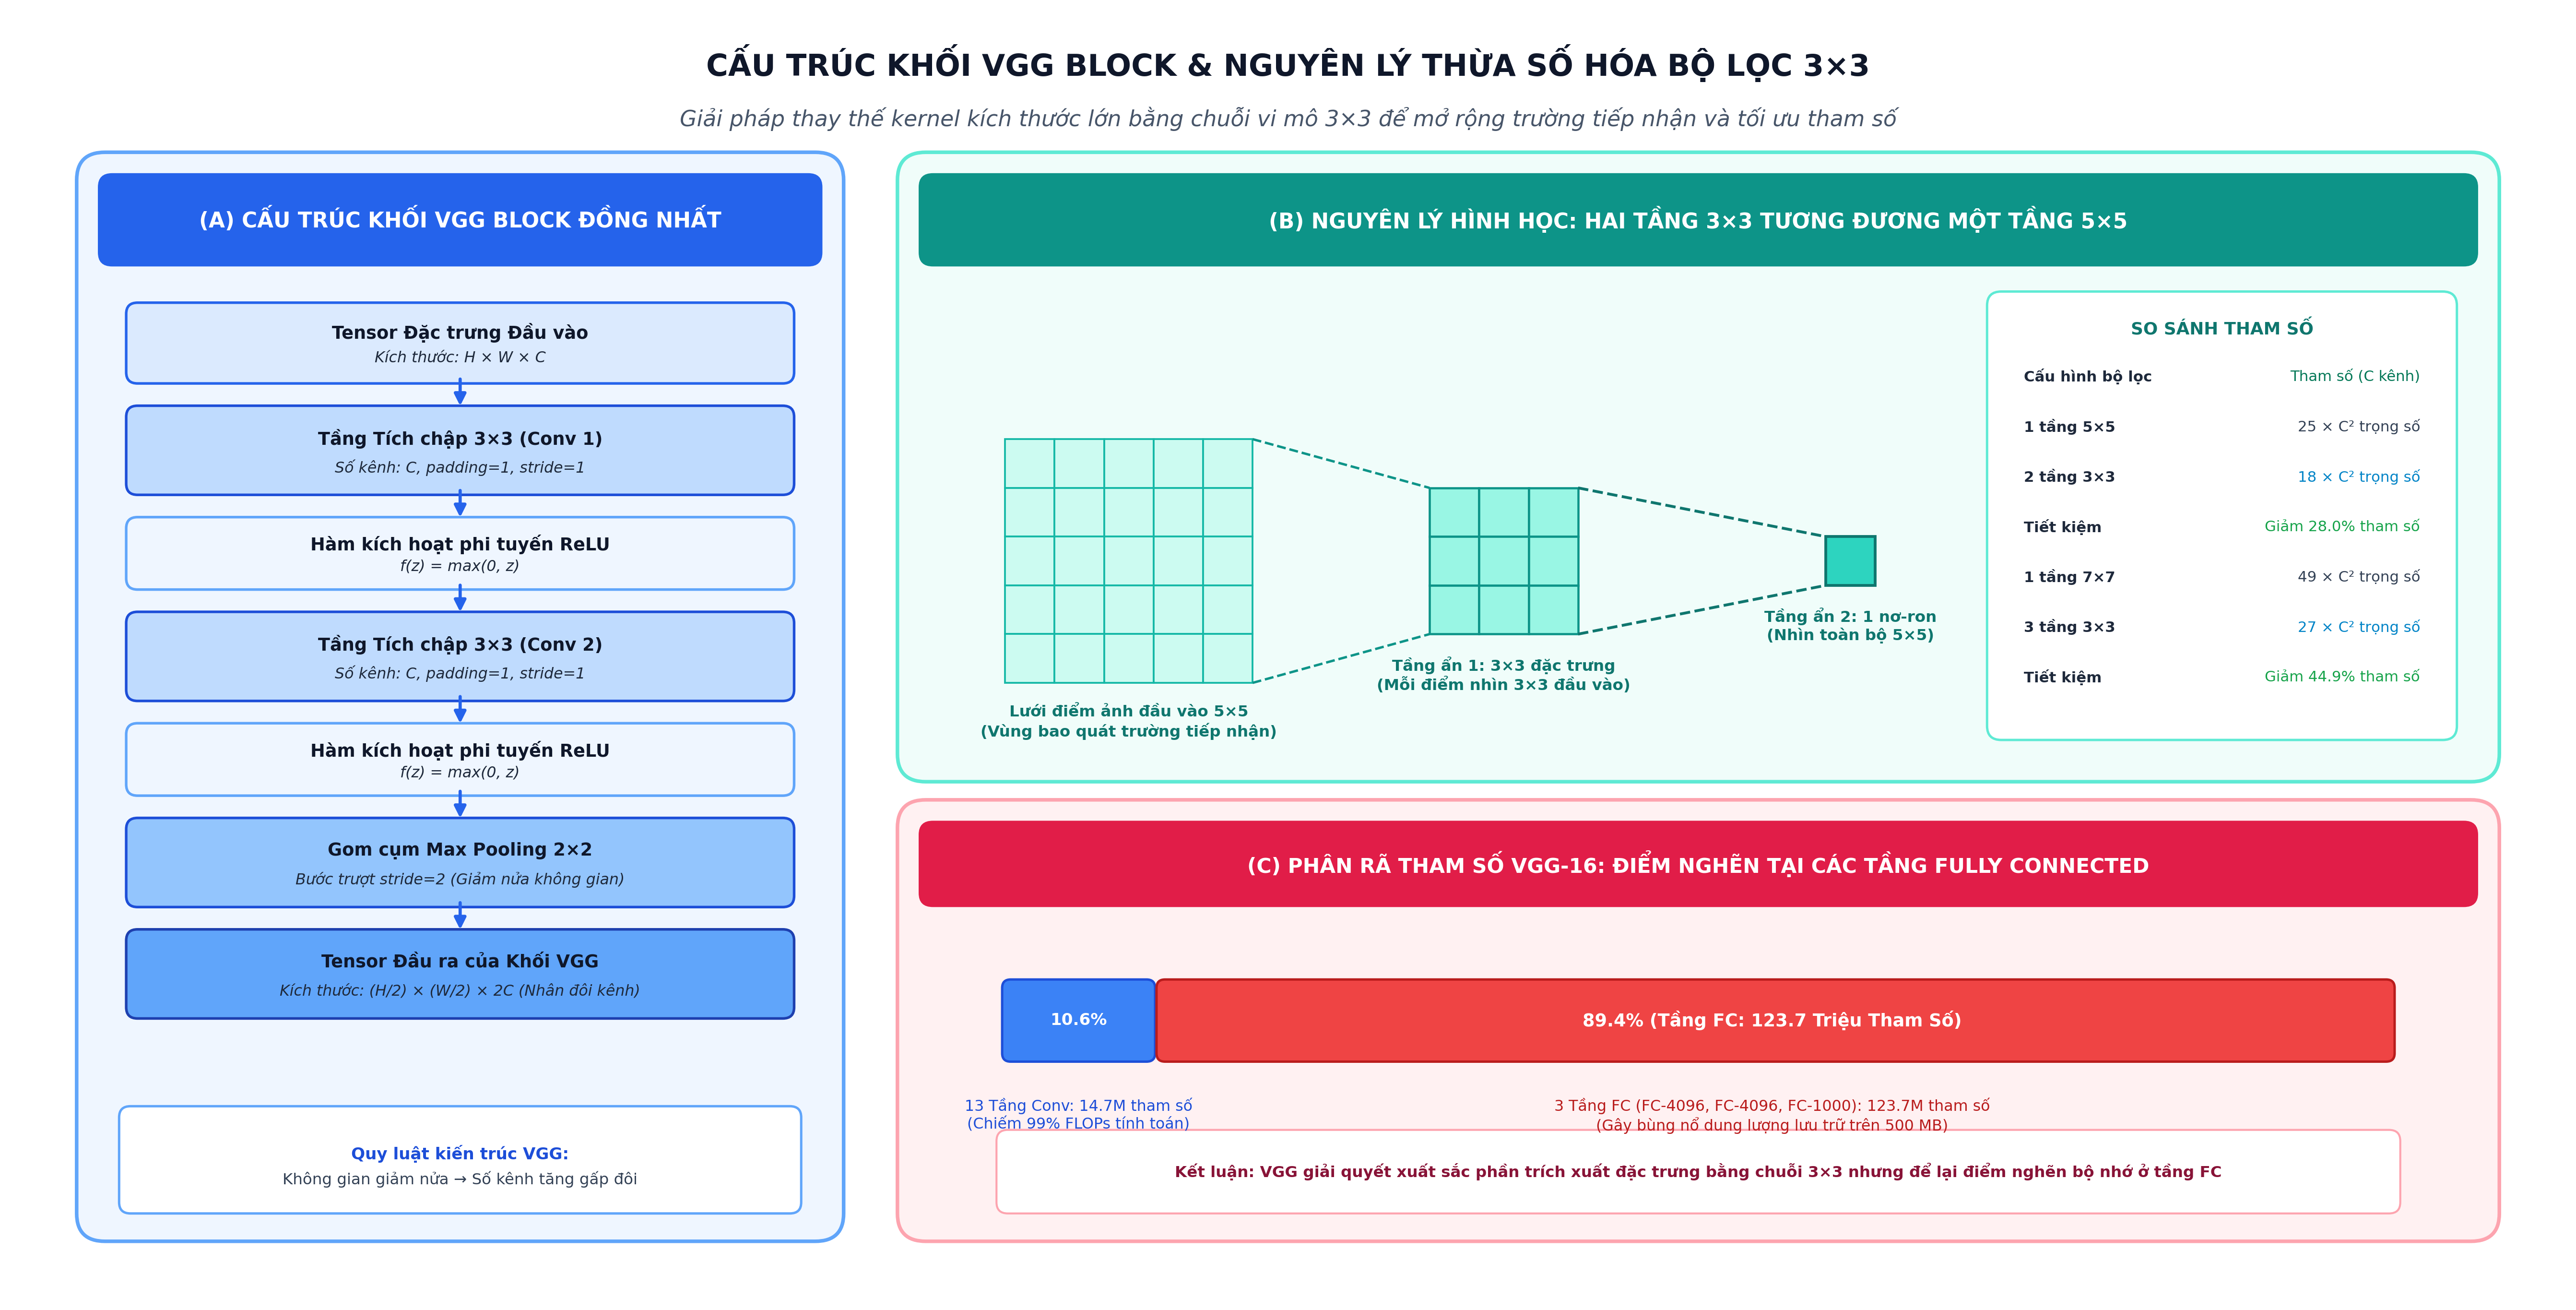
\includegraphics[width=0.92\textwidth]{images/fig202_vgg_block_and_receptive_field.png}
    \caption{Cấu trúc khối VGG và cơ chế tương đương kích thước đón nhận (Receptive Field).}
    \label{fig:vgg_block}
\end{figure}

\subsection{Nguyên Lý Vùng Đón Nhận Tương Đương (Equivalent Receptive Field)}
Cơ sở lý thuyết vững chắc nhất của việc thay thế các bộ lọc lớn bằng chuỗi các bộ lọc $3 \times 3$ nằm ở kích thước vùng đón nhận tương đương. Gọi $r_{l}$ là kích thước vùng đón nhận hiệu dụng của một nơ-ron tại tầng thứ $l$, công thức đệ quy tính vùng đón nhận khi xếp chồng các tầng tích chập có bước trượt $s=1$ được xác định theo:
\begin{equation}
    r_{l} = r_{l-1} + (k_l - 1)
\end{equation}
trong đó $k_l$ là kích thước kernel của tầng thứ $l$, và quy ước $r_0 = 1$ (tại điểm ảnh đầu vào).

\begin{itemize}[leftmargin=*]
    \item \textbf{Hai tầng tích chập $3 \times 3$ xếp chồng:}
    Tầng thứ nhất có $k_1 = 3 \implies r_1 = 1 + (3 - 1) = 3$. Tầng thứ hai có $k_2 = 3 \implies r_2 = 3 + (3 - 1) = 5$. Như vậy, hai tầng $3 \times 3$ liên tiếp tạo ra một vùng đón nhận kích thước $5 \times 5$ trên không gian đầu vào.

    \item \textbf{Ba tầng tích chập $3 \times 3$ xếp chồng:}
    Tầng thứ ba có $k_3 = 3 \implies r_3 = 5 + (3 - 1) = 7$. Như vậy, chuỗi ba tầng $3 \times 3$ liên tiếp tạo ra một vùng đón nhận kích thước hoàn toàn tương đương với một tầng tích chập đơn lẻ sử dụng bộ lọc $7 \times 7$.
\end{itemize}

Minh họa tại Hình \ref{fig:vgg_block} thể hiện trực quan quá trình lan tỏa thông tin không gian: điểm nơ-ron đơn lẻ tại tầng đầu ra thứ 3 tích hợp thông tin từ vùng $3 \times 3$ tại tầng 2, tương ứng với vùng $5 \times 5$ tại tầng 1, và bao quát trọn vẹn khu vực $7 \times 7$ tại ảnh đầu vào.

\subsection{Lợi Ích Kép: Năng Lực Phi Tuyến \& Tiết Kiệm Tham Số}
Việc phân rã một tầng $7 \times 7$ thành ba tầng $3 \times 3$ mang lại hai ưu thế vượt trội:

\begin{enumerate}[leftmargin=*]
    \item \textbf{Tăng cường độ phức tạp phi tuyến (Enhanced Non-Linearity):}
    Một tầng tích chập đơn lẻ kích thước $7 \times 7$ chỉ thực hiện một phép biến đổi tuyến tính kèm theo một hàm kích hoạt phi tuyến ReLU duy nhất. Ngược lại, chuỗi 3 tầng $3 \times 3$ tích hợp xen kẽ 3 hàm kích hoạt ReLU liên tiếp:
    \begin{equation}
        \mathbf{x}_3 = \operatorname{ReLU}\left(\mathbf{W}_3 * \operatorname{ReLU}\left(\mathbf{W}_2 * \operatorname{ReLU}\left(\mathbf{W}_1 * \mathbf{x}_0 + \mathbf{b}_1\right) + \mathbf{b}_2\right) + \mathbf{b}_3\right)
    \end{equation}
    Điều này cho phép hàm giả thuyết tổng thể phân tách các mặt quyết định (decision boundaries) phức tạp hơn rất nhiều, tăng cường đáng kể năng lực biểu diễn của mô hình.

    \item \textbf{Cắt giảm mạnh số lượng tham số tự do (Parameter Reduction):}
    Giả sử số kênh đầu vào và số kênh đầu ra cùng bằng $C$.
    \begin{itemize}
        \item Với một tầng tích chập $7 \times 7$, tổng số tham số trọng số là:
        \begin{equation}
            \Theta_{7 \times 7} = 7 \times 7 \times C \times C = 49 C^2
        \end{equation}
        \item Với ba tầng tích chập $3 \times 3$, tổng số tham số trọng số là:
        \begin{equation}
            \Theta_{3 \times (3 \times 3)} = 3 \times (3 \times 3 \times C \times C) = 27 C^2
        \end{equation}
        \item Tỷ số tham số giữa hai cách tiếp cận:
        \begin{equation}
            \frac{\Theta_{3 \times (3 \times 3)}}{\Theta_{7 \times 7}} = \frac{27 C^2}{49 C^2} = \frac{27}{49} \approx 55.1\%
        \end{equation}
    \end{itemize}
    Như vậy, việc thay thế một tầng $7 \times 7$ bằng ba tầng $3 \times 3$ giúp giảm tới \textbf{44.9\%} số lượng tham số trọng số, vừa giảm nguy cơ quá khớp (overfitting), vừa giảm dung lượng lưu trữ cần thiết cho mô hình.
\end{enumerate}

\subsection{Quy Tắc Nhân Đôi Số Kênh \& Cân Bằng Năng Lực Tính Toán}
VGG thiết lập nguyên lý cấu trúc không gian hình kim tự tháp chuẩn mực: cứ sau mỗi tầng Max Pooling $2 \times 2$ làm giảm một nửa chiều cao $H$ và chiều rộng $W$ của bản đồ đặc trưng, số lượng kênh $C$ sẽ được nhân đôi (từ $64 \to 128 \to 256 \to 512$). 

Quy tắc này giúp cân bằng khối lượng tính toán (FLOPs) giữa các giai đoạn (stages) của mạng. Khối lượng tính toán của một tầng tích chập chuẩn được tính xấp xỉ bởi:
\begin{equation}
    \text{FLOPs} \approx 2 \times H \times W \times C_{\text{in}} \times C_{\text{out}} \times k^2
\end{equation}
Khi kích thước không gian giảm 4 lần ($H/2 \times W/2$) và số kênh tăng gấp đôi ($C \to 2C$), tích số $(H/2) \cdot (W/2) \cdot (2C) \cdot (2C) = H \cdot W \cdot C^2$, nghĩa là khối lượng tính toán gần như được bảo toàn ổn định xuyên suốt các tầng sâu, không bị nghẽn cục bộ ở một giai đoạn đơn lẻ.

\subsection{Nút Thắt Cổ Chai \& Hạn Chế Của Kiến Trúc VGG}
Mặc dù là chuẩn mực thiết kế trong thời gian dài, VGG vẫn bộc lộ những điểm yếu chí mạng khiến nó dần bị thay thế trong các ứng dụng thực tế:
\begin{itemize}[leftmargin=*]
    \item \textbf{Nút thắt tham số tại các tầng Fully Connected (FC Layers):}
    Trong mô hình VGG-16 với tổng cộng 138.35 triệu tham số, ba tầng FC cuối cùng (FC-4096, FC-4096, FC-1000) chiếm tới hơn 123.6 triệu tham số (tương đương \textbf{89.3\%} toàn bộ tham số của mạng). Riêng tầng FC đầu tiên kết nối tensor đặc trưng đã trải phẳng $7 \times 7 \times 512 = 25,088$ nơ-ron với 4,096 nơ-ron ẩn đã tiêu tốn $25,088 \times 4096 \approx 102.76$ triệu trọng số.
    \item \textbf{Dung lượng bộ nhớ kích hoạt (Activation Memory):}
    Do duy trì độ phân giải cao ($224 \times 224$) qua nhiều tầng ở giai đoạn đầu, các bản đồ kích hoạt cần được lưu trữ trong bộ nhớ GPU trong quá trình lan truyền xuôi (Forward Pass) để phục vụ tính gradient ở quá trình lan truyền ngược (Backward Pass) lên tới hàng trăm Megabyte cho mỗi ảnh, gây khó khăn khi huấn luyện với kích thước batch lớn.
    \item \textbf{Giới hạn độ sâu (Vanishing Gradient):}
    Khi cố gắng mở rộng VGG vượt quá 19 tầng (như VGG-22 hay VGG-25), mô hình gặp phải hiện tượng gradient bị triệt tiêu khi lan truyền qua chuỗi dài các phép nhân ma trận, khiến sai số huấn luyện không thể hội tụ nếu không áp dụng các kỹ thuật khởi tạo cực kỳ khắt khe hoặc huấn luyện mồi (pre-training) trên mạng nông.
\end{itemize}


% =========================================================================
% 2.3. KIẾN TRÚC RESNET & ĐỘT PHÁ HỌC PHẦN DƯ
% =========================================================================
\section{Kiến Trúc ResNet \& Đột Phá Học Phần Dư (Residual Learning)}
\label{sec:resnet}

\subsection{Hiện Tượng Suy Biến Mạng Sâu (The Degradation Problem)}
Trước năm 2015, trực giác chung trong cộng đồng học sâu cho rằng việc tăng số lượng tầng sẽ trực tiếp làm tăng năng lực biểu diễn của mô hình. Tuy nhiên, các nghiên cứu thực nghiệm với các mạng tích chập sâu thuần túy (Plain Networks) cho thấy một nghịch lý nghiêm trọng: khi độ sâu mạng vượt quá khoảng 20 tầng, độ chính xác bắt đầu bão hòa và sau đó tụt dốc thảm hại.

Hiện tượng này được gọi là \textbf{Hiện tượng suy biến (Degradation Problem)}. Điều đặc biệt quan trọng là hiện tượng suy biến \textit{không phải do hiện tượng quá khớp (Overfitting)}. Trong thực nghiệm của He et al. (CVPR 2016), khi so sánh mạng 56 tầng và mạng 20 tầng thuần túy, mạng 56 tầng có cả sai số trên tập huấn luyện (training error) lẫn sai số trên tập kiểm tra (test error) đều cao hơn đáng kể so với mạng 20 tầng.

Về mặt lý thuyết, nếu không gian hàm biểu diễn của mạng sâu chứa không gian hàm của mạng nông, thì một mô hình 56 tầng hoàn toàn có thể đạt sai số huấn luyện không cao hơn mô hình 20 tầng đơn giản bằng cách sao chép 20 tầng của mạng nông và gán các tầng còn lại thành các phép ánh xạ đồng nhất (Identity Mappings, $f(\mathbf{x}) = \mathbf{x}$). Tuy nhiên, các thuật toán tối ưu hóa dựa trên gradient (SGD, Momentum, Adam) thực tế hoàn toàn thất bại trong việc tìm ra nghiệm đồng nhất này khi đi qua chuỗi dài các tầng tích chập phi tuyến.

\subsection{Khung Học Phần Dư (Deep Residual Learning Framework)}
Để phá vỡ nút thắt suy biến, Kaiming He cùng các cộng sự đã đề xuất khung học phần dư. Thay vì ép các tầng nơ-ron xếp chồng học trực tiếp ánh xạ mục tiêu phức tạp $\mathcal{H}(\mathbf{x})$, nhóm tác giả giả định rằng nếu ánh xạ tối ưu tiệm cận ánh xạ đồng nhất, thì việc học độ lệch phần dư sẽ dễ dàng hơn rất nhiều.

Đặt ánh xạ phần dư là:
\begin{equation}
    \mathcal{F}(\mathbf{x}) = \mathcal{H}(\mathbf{x}) - \mathbf{x}
\end{equation}
Khi đó, ánh xạ mục tiêu ban đầu được viết lại thành:
\begin{equation}
    \mathcal{H}(\mathbf{x}) = \mathcal{F}(\mathbf{x}) + \mathbf{x}
\end{equation}
Cấu trúc này được hiện thực hóa thông qua một \textbf{Khối Phần Dư (Residual Block)}, trong đó một \textbf{Đường truyền tắt đồng nhất (Identity Shortcut Connection)} nối tắt từ đầu vào $\mathbf{x}$, bỏ qua các tầng tích chập trung gian, và được cộng theo từng phần tử (element-wise addition) với đầu ra biến đổi $\mathcal{F}(\mathbf{x})$:
\begin{equation}
    \mathbf{y} = \sigma\left(\mathcal{F}(\mathbf{x}, \{\mathbf{W}_i\}) + \mathbf{x}\right)
\end{equation}
trong đó $\sigma(\cdot)$ là hàm kích hoạt ReLU đặt ở cuối khối, và $\mathcal{F}$ biểu diễn hàm ánh xạ phần dư được huấn luyện (thường bao gồm 2 hoặc 3 tầng Conv-BN-ReLU liên tiếp).

Nếu ánh xạ đồng nhất là cấu hình tối ưu, bộ tối ưu hóa chỉ cần triệt tiêu trọng số của các tầng tích chập về 0 ($\mathcal{F}(\mathbf{x}) \to \mathbf{0}$), đưa toàn bộ khối về ánh xạ đồng nhất $\mathbf{y} = \sigma(\mathbf{x})$. Việc đẩy trọng số về 0 thông qua kỹ thuật suy giảm trọng số (Weight Decay) dễ hơn theo cấp số nhân so với việc học phép biến đổi đồng nhất từ đầu.

\begin{figure}[H]
    \centering
    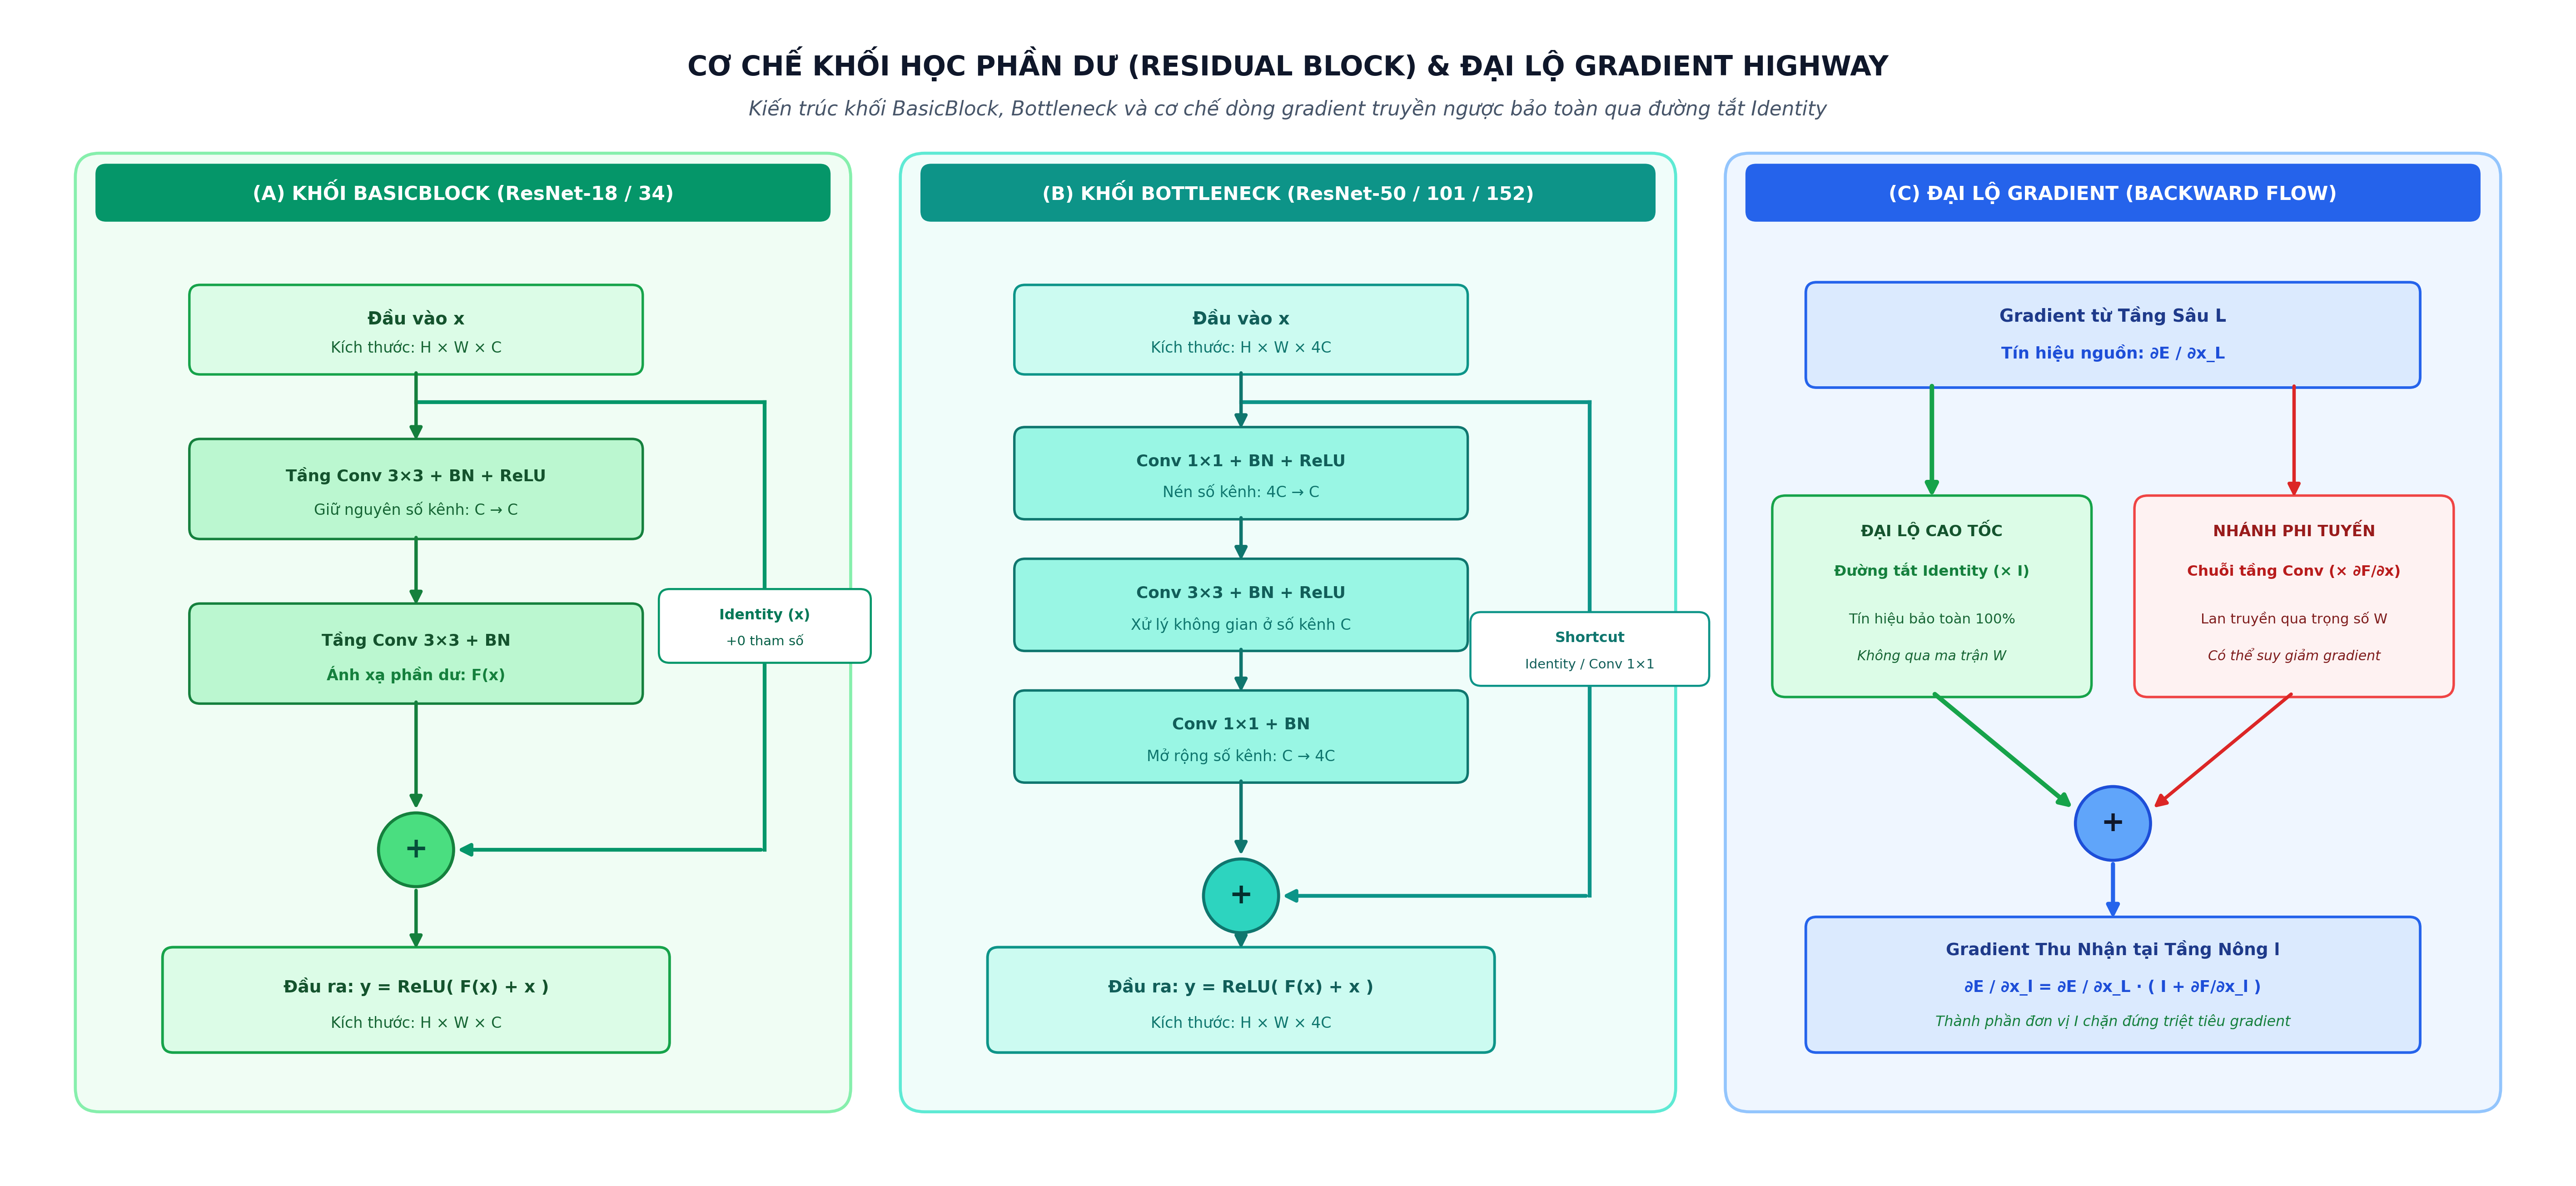
\includegraphics[width=0.95\textwidth]{images/fig203_resnet_residual_block_and_gradient.png}
    \caption{Cấu trúc khối ResNet Residual và cơ chế đại lộ gradient giải quyết suy biến mạng sâu.}
    \label{fig:resnet_block}
\end{figure}

\subsection{Giải Phẫu Toán Học: Đại Lộ Gradient (Gradient Highway)}
Bản chất kỳ diệu giúp ResNet có thể mở rộng độ sâu lên tới hàng trăm tầng (như ResNet-101, ResNet-152) nằm ở đặc tính lan truyền đạo hàm ngược qua đường tắt identity.

Xét một chuỗi gồm $L$ khối phần dư liên tiếp (với dạng pre-activation hoặc identity mapping). Đặc trưng tại tầng sâu $L$ có thể biểu diễn đệ quy dưới dạng tổng tích lũy từ tầng nông $l$ bất kỳ ($l < L$):
\begin{equation}
    \mathbf{x}_L = \mathbf{x}_l + \sum_{i=l}^{L-1} \mathcal{F}(\mathbf{x}_i, \mathcal{W}_i)
\end{equation}
Khi tính gradient của hàm mất mát toàn cục $\mathcal{E}$ theo đặc trưng đầu vào của tầng $l$ bằng quy tắc dây chuyền vi phân:
\begin{equation}
    \frac{\partial \mathcal{E}}{\partial \mathbf{x}_l} = \frac{\partial \mathcal{E}}{\partial \mathbf{x}_L} \cdot \frac{\partial \mathbf{x}_L}{\partial \mathbf{x}_l} = \frac{\partial \mathcal{E}}{\partial \mathbf{x}_L} \left( \mathbf{I} + \frac{\partial}{\partial \mathbf{x}_l} \sum_{i=l}^{L-1} \mathcal{F}(\mathbf{x}_i, \mathcal{W}_i) \right)
\end{equation}
Khai triển phương trình vi phân trên cho thấy gradient truyền ngược bao gồm hai thành phần rõ rệt:
\begin{equation}
    \frac{\partial \mathcal{E}}{\partial \mathbf{x}_l} = \underbrace{\frac{\partial \mathcal{E}}{\partial \mathbf{x}_L}}_{\text{Đại lộ Gradient trực tiếp}} + \underbrace{\frac{\partial \mathcal{E}}{\partial \mathbf{x}_L} \left(\frac{\partial}{\partial \mathbf{x}_l} \sum_{i=l}^{L-1} \mathcal{F}(\mathbf{x}_i, \mathcal{W}_i)\right)}_{\text{Thành phần gradient qua nhánh biến đổi}}
\end{equation}
\textbf{Ý nghĩa cốt lõi của ma trận đơn vị $\mathbf{I}$:}
\begin{itemize}[leftmargin=*]
    \item Gradient từ tầng sâu nhất $\frac{\partial \mathcal{E}}{\partial \mathbf{x}_L}$ có thể truyền \textbf{thẳng trực tiếp} về tầng nông nhất $\mathbf{x}_l$ mà không bị nhân liên tiếp qua bất kỳ ma trận trọng số $\mathcal{W}_i$ nào.
    \item Ngay cả khi thành phần tích chập $\frac{\partial}{\partial \mathbf{x}_l} \sum \mathcal{F}$ bị suy giảm triệt tiêu về 0 (vanishing), tổng gradient $\frac{\partial \mathcal{E}}{\partial \mathbf{x}_l}$ vẫn luôn giữ được giá trị khác không nhờ số hạng $\frac{\partial \mathcal{E}}{\partial \mathbf{x}_L} \mathbf{I}$.
    \item Do đó, hiện tượng biến mất gradient bị vô hiệu hóa hoàn toàn, biến đường truyền tắt thành một ``đại lộ cao tốc'' cho dòng gradient lưu thông tự do xuyên suốt toàn bộ chiều sâu của mạng nơ-ron.
\end{itemize}

\subsection{Hai Biến Thể Khối Phần Dư Cốt Lõi: BasicBlock \& BottleneckBlock}
Tùy thuộc vào độ sâu thiết kế của mạng, ResNet sử dụng hai biến thể khối phần dư:
\begin{enumerate}[leftmargin=*]
    \item \textbf{Khối cơ bản (BasicBlock - dùng cho ResNet-18, ResNet-34):}
    Bao gồm 2 tầng tích chập $3 \times 3$ liên tiếp kết hợp với Batch Normalization và hàm kích hoạt ReLU. Biến thể này phù hợp với các mạng có độ sâu vừa phải, nơi chi phí tính toán của kernel $3 \times 3$ trên số kênh hiện hành vẫn nằm trong giới hạn cho phép.
    \item \textbf{Khối thắt cổ chai (BottleneckBlock - dùng cho ResNet-50, ResNet-101, ResNet-152):}
    Khi số lượng kênh tăng lên tới 256 hoặc 512, chi phí tính toán của việc xếp chồng hai tầng $3 \times 3$ trở nên quá lớn. ResNet giải quyết bài toán này bằng cấu trúc 3 tầng:
    \begin{itemize}
        \item \textit{Tầng 1 ($1 \times 1$ Conv):} Nén (squeeze) số lượng kênh xuống 4 lần (ví dụ từ 256 xuống 64).
        \item \textit{Tầng 2 ($3 \times 3$ Conv):} Thực hiện trích xuất không gian trên không gian số chiều thấp (64 kênh).
        \item \textit{Tầng 3 ($1 \times 1$ Conv):} Mở rộng (expand) số lượng kênh trở lại 4 lần (từ 64 lên 256).
    \end{itemize}
    Cấu trúc thắt cổ chai này giúp giảm khối lượng tính toán FLOPs gần 3 lần so với việc duy trì 2 tầng $3 \times 3$ ở số kênh lớn, đồng thời cho phép mở rộng độ sâu mạng lên tới hơn 150 tầng với số tham số chỉ xấp xỉ 25.6 triệu (đối với ResNet-50).
\end{enumerate}

\subsection{Xử Lý Bất Đồng Kích Thước: Projection Shortcut}
Khi khối phần dư thực hiện chức năng giảm kích thước không gian (bước trượt $s=2$) hoặc mở rộng số kênh ($C_{\text{in}} \ne C_{\text{out}}$), tensor $\mathbf{x}$ và tensor $\mathcal{F}(\mathbf{x})$ không còn cùng kích thước hình học, khiến phép cộng phần tử không thể thực hiện trực tiếp.

Trong trường hợp này, ResNet sử dụng một \textbf{Phép chiếu tuyến tính (Projection Shortcut)}:
\begin{equation}
    \mathbf{y} = \mathcal{F}(\mathbf{x}, \{\mathbf{W}_i\}) + \mathbf{W}_s \mathbf{x}
\end{equation}
trong đó $\mathbf{W}_s$ là một phép tích chập $1 \times 1$ với bước trượt $s=2$ và số kênh ra bằng $C_{\text{out}}$, kết hợp ngay sau đó là một tầng Batch Normalization để đồng nhất tuyệt đối về cả kích thước không gian lẫn số kênh với nhánh chính.


% =========================================================================
% 2.4. KIẾN TRÚC MOBILENET & TÍCH CHẬP TÁCH RỜI CHIỀU SÂU
% =========================================================================
\section{Kiến Trúc MobileNet \& Tích Chập Tách Rời Chiều Sâu}
\label{sec:mobilenet}

\subsection{Bối Cảnh Điện Toán Biên \& Thách Thức Tài Nguyên}
Trong khi VGG và ResNet chủ yếu tập trung vào việc gia tăng độ chính xác trên các siêu máy chủ GPU, xu hướng ứng dụng thực tế của thị giác máy tính đòi hỏi các mô hình học sâu phải hoạt động hiệu quả trực tiếp trên các thiết bị biên (Edge Devices) có tài nguyên phần cứng cực kỳ hạn chế như điện thoại thông minh, hệ thống nhúng IoT, robot di động và xe tự hành. Các thiết bị này bị ràng buộc nghiêm ngặt bởi dung lượng RAM (thường dưới 1--2GB dành cho AI), năng lực xử lý số học dấu phẩy động (GFLOPS thấp), độ trễ phản hồi thời gian thực và thời lượng pin tiêu thụ.

Để giải quyết thách thức này, Howard et al. tại Google Research (2017) đã đề xuất kiến trúc \textbf{MobileNetV1}, dựa trên một giải pháp kiến trúc mang tính cách mạng: thay thế hoàn toàn phép tích chập chuẩn tốn kém bằng phép \textbf{Tích chập tách rời theo chiều sâu (Depthwise Separable Convolution)}.

\begin{figure}[H]
    \centering
    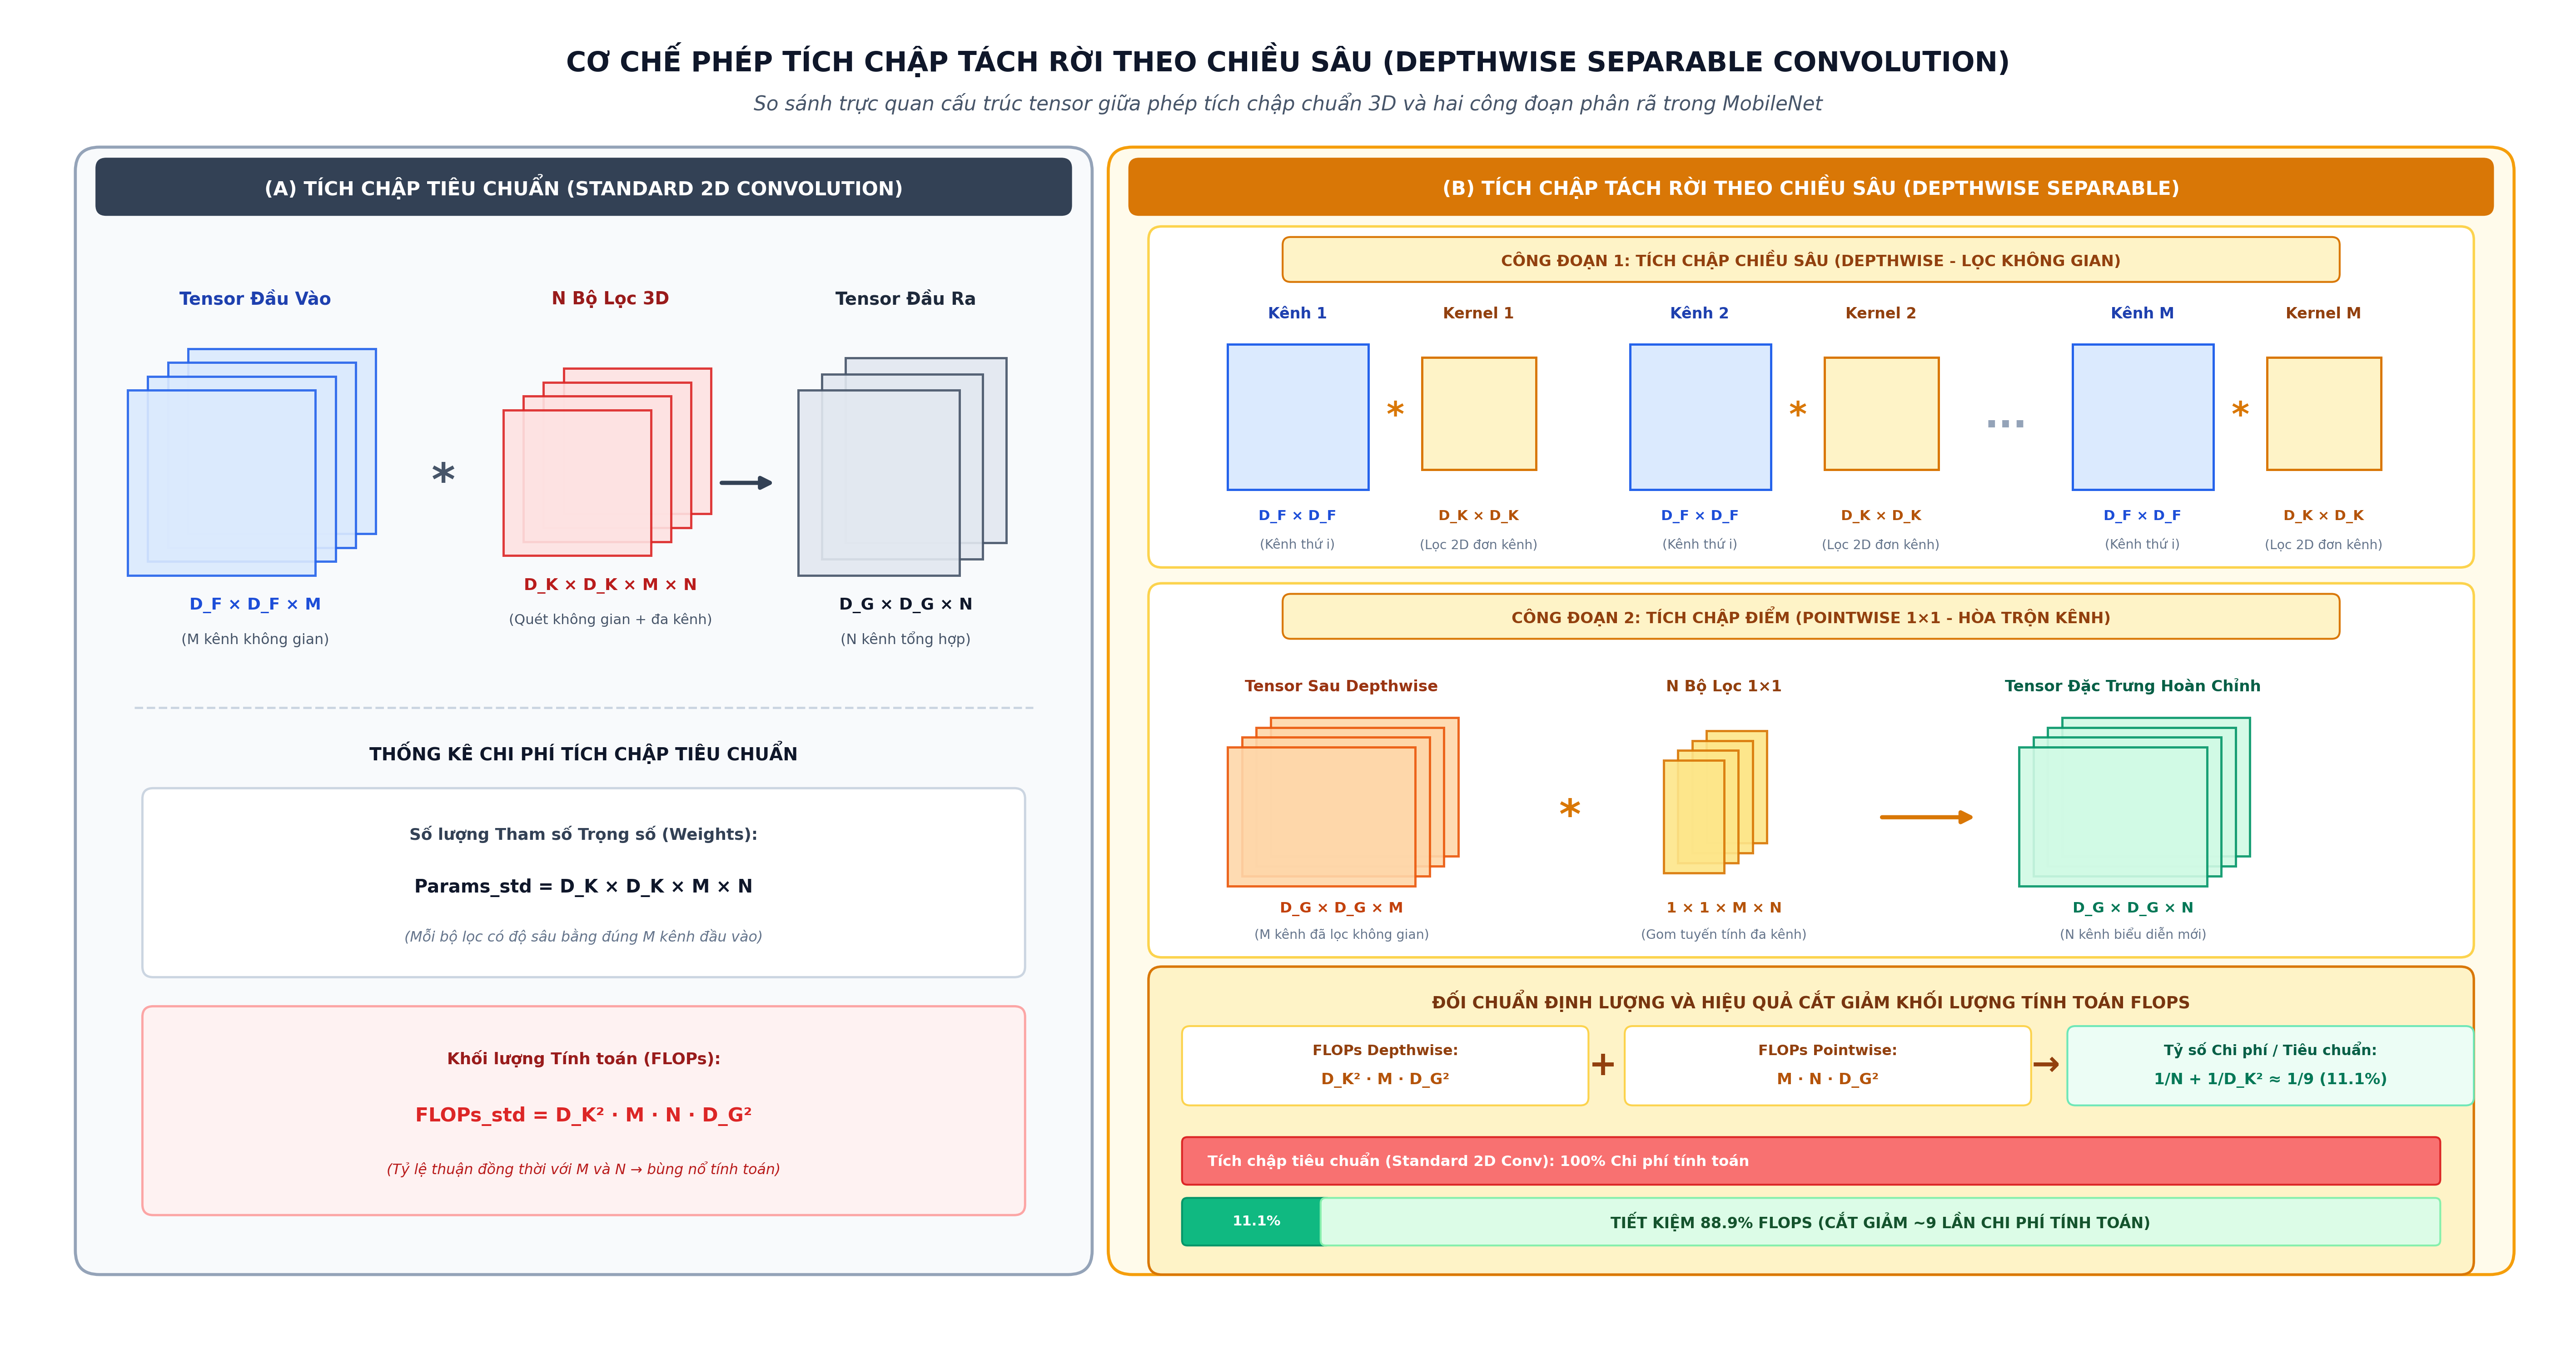
\includegraphics[width=0.95\textwidth]{images/fig204_mobilenet_depthwise_separable.png}
    \caption{Cơ chế tích chập tách rời chiều sâu (Depthwise Separable Convolution) trong \mbox{MobileNet}.}
    \label{fig:mobilenet_block}
\end{figure}

\subsection{Cơ Chế Tách Rời Chiều Sâu: Depthwise và Pointwise}
Phép tích chập chuẩn hai chiều thực hiện đồng thời hai nhiệm vụ trong một bước duy nhất: lọc các đặc trưng không gian trên từng kênh ($D_K \times D_K$) và kết hợp tuyến tính thông tin xuyên qua toàn bộ các kênh đầu vào ($M \to N$). Ý tưởng cốt lõi của Depthwise Separable Convolution là phân rã hai nhiệm vụ này thành hai công đoạn độc lập tuần tự (Hình \ref{fig:mobilenet_block}):

\begin{enumerate}[leftmargin=*]
    \item \textbf{Công đoạn 1 -- Depthwise Convolution (Lọc không gian theo từng kênh):}
    Áp dụng một bộ lọc không gian duy nhất kích thước $D_K \times D_K$ độc lập cho từng kênh đầu vào. Nếu tensor đầu vào có $M$ kênh, thì sẽ có đúng $M$ bộ lọc $D_K \times D_K$ hoạt động song song trên từng lát cắt 2D, hoàn toàn không có sự tương tác hay chia sẻ thông tin giữa các kênh với nhau. Đầu ra của công đoạn này là một tensor có kích thước $D_G \times D_G \times M$.
    \item \textbf{Công đoạn 2 -- Pointwise Convolution (Hòa trộn thông tin liên kênh):}
    Để kết hợp thông tin trích xuất từ các kênh khác nhau và điều chỉnh số lượng kênh từ $M$ sang $N$, MobileNet áp dụng phép tích chập điểm kích thước $1 \times 1$. Với $N$ bộ lọc kích thước $1 \times 1 \times M$, công đoạn này tính tổ hợp tuyến tính xuyên qua toàn bộ $M$ kênh tại từng vị trí không gian để tạo ra tensor đặc trưng hoàn chỉnh kích thước $D_G \times D_G \times N$.
\end{enumerate}

Mỗi công đoạn tích chập trong khối đều được tiếp nối ngay bởi một tầng Batch Normalization và một hàm kích hoạt phi tuyến ReLU6.

\subsection{Chứng Minh Định Lượng Mức Độ Tiết Kiệm FLOPs \& Tham Số}
Gọi:
\begin{itemize}
    \item $D_F \times D_F \times M$: Kích thước không gian và số kênh của tensor đầu vào.
    \item $D_G \times D_G \times N$: Kích thước không gian và số kênh của tensor đầu ra.
    \item $D_K \times D_K$: Kích thước không gian của bộ lọc tích chập (thường $D_K = 3$).
\end{itemize}

\subsubsection{Khối Lượng Tính Toán Của Tích Chập Chuẩn}
Một phép tích chập chuẩn sử dụng $N$ bộ lọc kích thước $D_K \times D_K \times M$. Tại mỗi vị trí không gian của bản đồ đặc trưng đầu ra ($D_G \times D_G$), để tạo ra một giá trị kích hoạt cho 1 kênh cần $D_K \times D_K \times M$ phép nhân và cộng. Với $N$ kênh đầu ra, tổng số phép tính dấu phẩy động (FLOPs) là:
\begin{equation}
    \text{FLOPs}_{\text{std}} = D_K \cdot D_K \cdot M \cdot N \cdot D_G \cdot D_G
\end{equation}
Số lượng tham số trọng số tương ứng là:
\begin{equation}
    \Theta_{\text{std}} = D_K \cdot D_K \cdot M \cdot N
\end{equation}

\subsubsection{Khối Lượng Tính Toán Của Tích Chập Tách Rời Chiều Sâu}
Khối lượng tính toán của tích chập tách rời chiều sâu bằng tổng của hai công đoạn:
\begin{enumerate}
    \item Chi phí của tầng Depthwise ($M$ bộ lọc kích thước $D_K \times D_K \times 1$):
    \begin{equation}
        \text{FLOPs}_{\text{dw}} = D_K \cdot D_K \cdot M \cdot D_G \cdot D_G
    \end{equation}
    \item Chi phí của tầng Pointwise ($N$ bộ lọc kích thước $1 \times 1 \times M$):
    \begin{equation}
        \text{FLOPs}_{\text{pw}} = 1 \cdot 1 \cdot M \cdot N \cdot D_G \cdot D_G
    \end{equation}
\end{enumerate}
Tổng chi phí tính toán của toàn bộ khối tách rời chiều sâu là:
\begin{equation}
    \text{FLOPs}_{\text{dws}} = \text{FLOPs}_{\text{dw}} + \text{FLOPs}_{\text{pw}} = D_K \cdot D_K \cdot M \cdot D_G \cdot D_G + M \cdot N \cdot D_G \cdot D_G
\end{equation}
Tổng số tham số trọng số tương ứng là:
\begin{equation}
    \Theta_{\text{dws}} = D_K \cdot D_K \cdot M + M \cdot N
\end{equation}

\subsubsection{Tỷ Số Tiết Kiệm Toán Học}
Lấy tỷ số giữa khối lượng tính toán của tích chập tách rời chiều sâu so với tích chập chuẩn:
\begin{equation}
    \frac{\text{FLOPs}_{\text{dws}}}{\text{FLOPs}_{\text{std}}} = \frac{D_K^2 \cdot M \cdot D_G^2 + M \cdot N \cdot D_G^2}{D_K^2 \cdot M \cdot N \cdot D_G^2} = \frac{D_K^2 + N}{D_K^2 \cdot N} = \frac{1}{N} + \frac{1}{D_K^2}
\end{equation}
Tương tự đối với tỷ số số lượng tham số trọng số:
\begin{equation}
    \frac{\Theta_{\text{dws}}}{\Theta_{\text{std}}} = \frac{D_K^2 \cdot M + M \cdot N}{D_K^2 \cdot M \cdot N} = \frac{1}{N} + \frac{1}{D_K^2}
\end{equation}
Trong các kiến trúc thực tế, kích thước bộ lọc tiêu chuẩn là $D_K = 3$, và số kênh đầu ra thường rất lớn ($N \ge 64, 128, 512, 1024$). Khi đó, số hạng $\frac{1}{N} \ll 1$ và có thể bỏ qua khi xấp xỉ:
\begin{equation}
    \frac{\text{FLOPs}_{\text{dws}}}{\text{FLOPs}_{\text{std}}} \approx \frac{1}{D_K^2} = \frac{1}{3^2} = \frac{1}{9} \approx 11.1\%
\end{equation}
\textbf{Kết luận:} Việc áp dụng tích chập tách rời theo chiều sâu giúp \textbf{cắt giảm từ 8 đến 9 lần (khoảng 89\%)} cả khối lượng tính toán FLOPs lẫn số lượng tham số bộ lọc so với tích chập chuẩn. Đáng kinh ngạc hơn, kết quả thực nghiệm trên tập ImageNet cho thấy sự suy giảm độ chính xác Top-1 chỉ xấp xỉ khoảng $1\%$ so với việc sử dụng toàn bộ tích chập chuẩn!

\subsection{Hai Siêu Tham Số Co Giãn Mô Hình (Model Shrinking Hyperparameters)}
Để tăng tính linh hoạt khi triển khai trên các thiết bị phần cứng có cấu hình đa dạng, MobileNetV1 đưa vào hai siêu tham số toàn cục điều chỉnh sự đánh đổi giữa độ chính xác và tốc độ xử lý:

\begin{itemize}[leftmargin=*]
    \item \textbf{Hệ số co giãn chiều rộng (Width Multiplier $\alpha \in (0, 1]$):}
    Điều chỉnh đồng đều số lượng kênh tại tất cả các tầng của mạng. Số kênh đầu vào $M$ trở thành $\alpha M$, và số kênh đầu ra $N$ trở thành $\alpha N$. Khối lượng tính toán của khối biến đổi theo:
    \begin{equation}
        \text{FLOPs}(\alpha) = D_K^2 \cdot (\alpha M) \cdot D_G^2 + (\alpha M) \cdot (\alpha N) \cdot D_G^2 \approx \alpha^2 \cdot \text{FLOPs}_{\text{dws}}
    \end{equation}
    Như vậy, khi chọn $\alpha = 0.5$, số lượng tham số và khối lượng tính toán giảm xấp xỉ 4 lần ($\alpha^2 = 0.25$), tạo ra một mô hình siêu nhẹ cho các bộ vi xử lý cấp thấp.

    \item \textbf{Hệ số co giãn độ phân giải (Resolution Multiplier $\rho \in (0, 1]$):}
    Điều chỉnh độ phân giải của ảnh đầu vào và các bản đồ đặc trưng không gian: $D_F \to \rho D_F$ và $D_G \to \rho D_G$. Khối lượng tính toán tỷ lệ với diện tích không gian:
    \begin{equation}
        \text{FLOPs}(\alpha, \rho) \approx \alpha^2 \cdot \rho^2 \cdot \text{FLOPs}_{\text{dws}}
    \end{equation}
    Hệ số này không làm thay đổi số lượng tham số trọng số lưu trữ nhưng giúp giảm đáng kể thời gian xử lý và dung lượng RAM tức thời trong pha suy luận.
\end{itemize}

\subsection{Hàm Kích Hoạt ReLU6 \& Tối Ưu Hóa Số Học Điểm Tĩnh (Fixed-Point)}
Khác với ReLU truyền thống ($\operatorname{ReLU}(x) = \max(0, x)$) không có giới hạn trên, MobileNet sử dụng hàm kích hoạt \textbf{ReLU6}:
\begin{equation}
    \operatorname{ReLU6}(x) = \min(\max(0, x), 6)
\end{equation}
\textbf{Căn cứ thiết kế kỹ thuật:}
Trên các vi xử lý di động hoặc chip nhúng DSP, các mô hình học sâu thường được lượng tử hóa từ định dạng số thực dấu phẩy động 32-bit (FP32) sang định dạng số nguyên 8-bit (INT8) để tăng tốc xử lý và tiết kiệm pin. Khi hàm kích hoạt không bị chặn trên, một số giá trị ngoại lai (outliers) quá lớn sẽ làm dải động bị kéo giãn, dẫn đến mất mát độ chính xác nghiêm trọng tại các vùng giá trị nhỏ. Việc chặn cứng giá trị kích hoạt tối đa ở mức 6.0 giúp dải biểu diễn số học điểm tĩnh bảo toàn được tối đa độ phân giải thông tin ở các giá trị đặc trưng thấp, đảm bảo mô hình giữ vững độ chính xác sau quá trình lượng tử hóa.


% =========================================================================
% 2.5. PHÂN TÍCH SO SÁNH ĐỊNH LƯỢNG GIỮA BA KHỐI KIẾN TRÚC
% =========================================================================
\section{Phân Tích So Sánh Định Lượng Giữa Ba Khối Kiến Trúc}
Để cung cấp một góc nhìn phân tích tổng hợp và hệ thống hóa, Bảng \ref{tab:chapter2_block_comparison} đối chuẩn trực diện ba khối kiến trúc cốt lõi (VGG Block, ResNet BasicBlock, và MobileNet SeparableBlock) trên các tiêu chí toán học, độ phức tạp tính toán, cơ chế lan truyền đạo hàm và môi trường ứng dụng thực tế.

\begin{table}[H]
\centering
\small
\caption{Bảng so sánh đối chuẩn định lượng giữa ba khối kiến trúc CNN kinh điển}
\label{tab:chapter2_block_comparison}
\renewcommand{\arraystretch}{1.32}
\setlength{\tabcolsep}{4.5pt}
\begin{tabularx}{\textwidth}{>{\bfseries\raggedright\arraybackslash}p{3.3cm} >{\raggedright\arraybackslash}X >{\raggedright\arraybackslash}X >{\raggedright\arraybackslash}X}
\toprule
\rowcolor{blue!85!black}
\textcolor{white}{\textbf{Tiêu chí đối chuẩn}} & 
\textcolor{white}{\textbf{VGG Block}} & 
\textcolor{white}{\textbf{ResNet BasicBlock}} & 
\textcolor{white}{\textbf{MobileNet Separable}} \\
\midrule
% -------------------------------------------------------------
\rowcolor{blue!8}
\multicolumn{4}{l}{\bfseries\color{blue!90!black} I. CẤU TRÚC TẦNG \& CÔNG THỨC TOÁN HỌC} \\
\midrule
Cấu trúc các tầng & 
$\bullet$ $[\text{Conv } 3\times 3 \to \text{BN} \to \text{ReLU}] \times 2$ \newline
$\bullet$ $\text{MaxPool } 2\times 2$ ($s=2$) & 
$\bullet$ $\text{Conv } 3\times 3 \to \text{BN} \to \text{ReLU}$ \newline
$\bullet$ $\text{Conv } 3\times 3 \to \text{BN}$ \newline
$+$ Nhánh tắt $(\mathbf{x}) \to \text{ReLU}$ & 
$\bullet$ $\text{DW Conv } 3\times 3 \to \text{BN} \to \text{ReLU6}$ \newline
$\bullet$ $\text{PW Conv } 1\times 1 \to \text{BN} \to \text{ReLU6}$ \\

\rowcolor{gray!4}
Công thức tham số & 
$2 \times (3^2 \cdot C_{\text{in}} \cdot C_{\text{out}})$ & 
$3^2 C_{\text{in}} C_{\text{out}} + 3^2 C_{\text{out}}^2 + (C_{\text{in}} C_{\text{out}})^{\dagger}$ & 
$3^2 C_{\text{in}} + C_{\text{in}} C_{\text{out}}$ \\

Công thức FLOPs & 
$2 \cdot 3^2 C_{\text{in}} C_{\text{out}} H W$ & 
$(3^2 C_{\text{in}} C_{\text{out}} + 3^2 C_{\text{out}}^2)HW$ \newline
$+ (C_{\text{in}} C_{\text{out}})HW \text{ (proj)}$ & 
$(3^2 C_{\text{in}} + C_{\text{in}} C_{\text{out}}) H W$ \\
\midrule
% -------------------------------------------------------------
\rowcolor{blue!8}
\multicolumn{4}{l}{\bfseries\color{blue!90!black} II. ĐỐI CHUẨN THỰC NGHIỆM ($C_{\text{in}}=64 \to C_{\text{out}}=128, s=2$)} \\
\midrule
Tham số thực nghiệm & 
\textbf{221,440} \newline
\textcolor{gray!80!black}{(100\% -- chuẩn đối sánh)} & 
\textbf{230,144} \newline
\textcolor{gray!80!black}{(103.9\% do nhánh chiếu)} & 
\textbf{9,152} \newline
\colorbox{green!15}{\textcolor{green!60!black}{\bfseries 4.13\% (giảm 95.87\%)}} \\

\rowcolor{gray!4}
Bộ nhớ kích hoạt & 
Cao \newline
\textit{\footnotesize (Lưu giữ tensor 2D lớn)} & 
Trung bình \newline
\textit{\footnotesize (Lưu trữ nhánh skip connection)} & 
Rất thấp \newline
\textit{\footnotesize (Tách kênh giảm tải bộ đệm)} \\
\midrule
% -------------------------------------------------------------
\rowcolor{blue!8}
\multicolumn{4}{l}{\bfseries\color{blue!90!black} III. ĐỘNG HỌC HỌC SÂU \& TRIỂN KHAI THỰC TẾ} \\
\midrule
Dòng truyền Gradient & 
Nhân chuỗi Jacobian $\prod_{i} \mathbf{J}_i$ \newline
\textcolor{red!70!black}{\footnotesize Nguy cơ triệt tiêu ở mạng sâu} & 
Đại lộ cộng trực tiếp $\mathbf{I} + \frac{\partial \mathcal{F}}{\partial \mathbf{x}}$ \newline
\textcolor{blue!80!black}{\footnotesize Bảo toàn gradient tuyệt đối} & 
Chuỗi nhân ngắn qua DW và PW \newline
\textcolor{green!60!black}{\footnotesize Ổn định, ít bị suy thoái} \\

\rowcolor{gray!4}
Mục tiêu kiến trúc & 
Chuẩn hóa không gian đón nhận bằng kernel nhỏ $3\times 3$ & 
Giải phóng giới hạn độ sâu, tránh suy thoái biểu diễn & 
Cắt giảm tối đa FLOPs và bộ nhớ cho thiết bị biên \\

Phần cứng mục tiêu & 
Máy chủ GPU hiệu năng cao (Server / HPC) & 
Máy chủ GPU, trung tâm dữ liệu huấn luyện sâu & 
Mobile, Edge AI, IoT, Raspberry Pi, nhúng \\
\bottomrule
\end{tabularx}
\vspace{1.5mm}
\begin{tcolorbox}[colback=blue!2, colframe=blue!20, arc=1mm, boxrule=0.5pt, left=2mm, right=2mm, top=1mm, bottom=1mm]
\footnotesize\itshape $^{\dagger}$ \textbf{Ghi chú:} $(C_{\text{in}} C_{\text{out}})$ là số lượng tham số bổ sung của tầng Conv $1 \times 1$ trong nhánh tắt chiếu (Projection Shortcut), được kích hoạt khi khối thực hiện đồng thời hai nhiệm vụ: giảm một nửa độ phân giải không gian ($s=2$) và nhân đôi số kênh đặc trưng ($64 \to 128$).
\end{tcolorbox}
\end{table}


% =========================================================================
% 2.6. HIỆN THỰC HÓA MÃ NGUỒN PYTORCH MODULE HÓA & KIỂM CHỨNG SỐ TRỊ
% =========================================================================
\section{Hiện Thực Hóa Mã Nguồn PyTorch Module Hóa \& Kiểm Chứng Số Trị}

\subsection{Mã Nguồn Cài Đặt Module Hóa Ba Khối Kiến Trúc}
Nhằm kiểm chứng chính xác các nguyên lý lý thuyết đã trình bày, chúng tôi hiện thực hóa cả ba khối kiến trúc bằng thư viện PyTorch dưới dạng các lớp kế thừa từ \texttt{torch.nn.Module} chuẩn mực, đảm bảo tính tái sử dụng cao và hoàn toàn tương thích với các bộ tối ưu hóa hiện đại. Đoạn mã dưới đây minh họa việc cài đặt chi tiết của từng khối.

\begin{lstlisting}[language=Python, caption={Cài đặt module hóa ba khối kiến trúc VGG, ResNet và MobileNet trong PyTorch}]
import torch
import torch.nn as nn

# 1. Khoi VGG Block Dong Nhat (2x Conv 3x3 + MaxPool 2x2)
class VGGBlock(nn.Module):
    def __init__(self, in_channels: int, out_channels: int, num_convs: int = 2):
        super().__init__()
        layers = []
        for i in range(num_convs):
            c_in = in_channels if i == 0 else out_channels
            layers.extend([
                nn.Conv2d(c_in, out_channels, kernel_size=3, stride=1, padding=1, bias=True),
                nn.BatchNorm2d(out_channels),
                nn.ReLU(inplace=True)
            ])
        layers.append(nn.MaxPool2d(kernel_size=2, stride=2))
        self.block = nn.Sequential(*layers)

    def forward(self, x: torch.Tensor) -> torch.Tensor:
        return self.block(x)


# 2. Khoi ResNet BasicBlock voi Duong Truyen Tat Phan Du
class ResidualBlock(nn.Module):
    def __init__(self, in_channels: int, out_channels: int, stride: int = 1):
        super().__init__()
        # Nhanh bien doi F(x)
        self.conv1 = nn.Conv2d(in_channels, out_channels, kernel_size=3, stride=stride, padding=1, bias=False)
        self.bn1 = nn.BatchNorm2d(out_channels)
        self.relu = nn.ReLU(inplace=True)
        self.conv2 = nn.Conv2d(out_channels, out_channels, kernel_size=3, stride=1, padding=1, bias=False)
        self.bn2 = nn.BatchNorm2d(out_channels)

        # Nhanh Projection Shortcut khi bat dong kich thuoc
        if stride != 1 or in_channels != out_channels:
            self.shortcut = nn.Sequential(
                nn.Conv2d(in_channels, out_channels, kernel_size=1, stride=stride, bias=False),
                nn.BatchNorm2d(out_channels)
            )
        else:
            self.shortcut = nn.Identity()

    def forward(self, x: torch.Tensor) -> torch.Tensor:
        residual = self.shortcut(x)
        out = self.relu(self.bn1(self.conv1(x)))
        out = self.bn2(self.conv2(out))
        out += residual
        return self.relu(out)


# 3. Khoi MobileNet Depthwise Separable Block
class DepthwiseSeparableBlock(nn.Module):
    def __init__(self, in_channels: int, out_channels: int, stride: int = 1):
        super().__init__()
        # Depthwise Convolution: groups = in_channels
        self.depthwise = nn.Sequential(
            nn.Conv2d(in_channels, in_channels, kernel_size=3, stride=stride, padding=1,
                      groups=in_channels, bias=False),
            nn.BatchNorm2d(in_channels),
            nn.ReLU6(inplace=True)
        )
        # Pointwise Convolution: 1x1 Conv
        self.pointwise = nn.Sequential(
            nn.Conv2d(in_channels, out_channels, kernel_size=1, stride=1, padding=0, bias=False),
            nn.BatchNorm2d(out_channels),
            nn.ReLU6(inplace=True)
        )

    def forward(self, x: torch.Tensor) -> torch.Tensor:
        x = self.depthwise(x)
        x = self.pointwise(x)
        return x
\end{lstlisting}

\subsection{Kịch Bản Kiểm Chứng Luồng Tensor \& Ổn Định Gradient}
Để kiểm chứng thực nghiệm tính đúng đắn toán học và hành vi số trị của ba khối, chúng tôi thiết lập một kịch bản thử nghiệm đồng nhất:
\begin{itemize}[leftmargin=*]
    \item \textbf{Tensor đầu vào:} Batch gồm $B=2$ mẫu, số kênh $C_{\text{in}}=64$, kích thước không gian $H \times W = 32 \times 32$. Tensor được khởi tạo ngẫu nhiên theo phân phối chuẩn tắc với cờ theo dõi vi phân \texttt{requires\_grad=True}.
    \item \textbf{Mục tiêu cấu hình:} Chuyển đổi số kênh từ $64 \to 128$ đồng thời giảm kích thước không gian đi một nửa ($32 \times 32 \to 16 \times 16$, bước trượt hiệu dụng $s=2$).
    \item \textbf{Đánh giá lan truyền ngược:} Khởi tạo hàm mất mát vô hướng $\mathcal{L} = \sum \mathbf{y}_{\text{out}}$, thực thi lan truyền ngược bằng \texttt{loss.backward()}, và đo lường chuẩn đạo hàm cấp hai (L2-norm) của gradient truyền ngược về tensor đầu vào:
    \begin{equation}
        \|\nabla_{\mathbf{x}} \mathcal{L}\|_2 = \sqrt{\sum_{i} \left(\frac{\partial \mathcal{L}}{\partial x_i}\right)^2}
    \end{equation}
\end{itemize}

\begin{table}[H]
\centering
\small
\caption{Kết quả kiểm chứng định lượng luồng tensor và đạo hàm của 3 khối kiến trúc}
\label{tab:pytorch_verification_results}
\begin{tabularx}{\textwidth}{lccccc}
\toprule
\textbf{Khối kiến trúc} & \textbf{Shape đầu vào} & \textbf{Shape đầu ra} & \textbf{Số tham số} & \textbf{Tỷ lệ tham số} & \textbf{Chuẩn đạo hàm $\|\nabla_{\mathbf{x}} \mathcal{L}\|_2$} \\
\midrule
\textbf{VGG Block} & $[2, 64, 32, 32]$ & $[2, 128, 16, 16]$ & $221,440$ & $100.00\%$ & $73.4735$ \\
\addlinespace
\textbf{Residual Block} & $[2, 64, 32, 32]$ & $[2, 128, 16, 16]$ & $230,144$ & $103.93\%$ & $164.0931$ \\
\addlinespace
\textbf{MobileNet Block} & $[2, 64, 32, 32]$ & $[2, 128, 16, 16]$ & $\mathbf{9,152}$ & $\mathbf{4.13\%}$ & $97.9947$ \\
\bottomrule
\end{tabularx}
\end{table}

\subsection{Phân Tích Đánh Giá Kết Quả Kiểm Chứng}
Kết quả thực nghiệm số trị tại Bảng \ref{tab:pytorch_verification_results} khẳng định các kết luận lý thuyết quan trọng sau:
\begin{enumerate}[leftmargin=*]
    \item \textbf{Tính nhất quán về hình học tensor:} Cả 3 khối đều chuyển đổi thành công tensor đầu vào $[2, 64, 32, 32]$ về đúng kích thước mong muốn $[2, 128, 16, 16]$, chứng minh tính tương thích hoàn hảo của các cơ chế giảm kích thước không gian khác nhau (VGG dùng MaxPool, ResNet dùng Conv $3\times 3$ stride 2 kèm shortcut $1\times 1$, MobileNet dùng DW Conv $3\times 3$ stride 2).
    \item \textbf{Mức độ cắt giảm tham số đột phá của MobileNet:} Khối Separable Block của MobileNet chỉ tiêu tốn đúng \textbf{9,152 tham số}, giảm tới \textbf{95.87\%} so với khối VGG (221,440 tham số) và giảm \textbf{96.02\%} so với khối ResNet (230,144 tham số). Đây là bằng chứng thực nghiệm rõ nét cho sức mạnh tối ưu của phép tách rời chiều sâu khi triển khai trên phần cứng giới hạn.
    \item \textbf{Sự ổn định và sức mạnh của dòng Gradient trong ResNet:} Chuẩn gradient truyền ngược về đầu vào của Residual Block đạt mức cao nhất ($164.0931$), cao hơn gấp 2.23 lần so với VGG Block ($73.4735$). Điều này chứng minh trên phương diện số trị rằng đường truyền tắt shortcut đóng góp một lượng lớn gradient trực tiếp không suy giảm ($\frac{\partial \mathcal{E}}{\partial \mathbf{x}_L} \mathbf{I}$), giúp các tầng sâu nhận được tín hiệu cập nhật mạnh mẽ và ổn định.
    \item \textbf{Không có hiện tượng bão hòa hay phát nổ gradient:} Toàn bộ các khối đều cho chuẩn đạo hàm hữu hạn, không xuất hiện hiện tượng giá trị vô cực (\texttt{Inf}) hoặc giá trị không xác định (\texttt{NaN}), sẵn sàng cho quá trình tối ưu hóa ổn định trong toàn bộ mạng.
\end{enumerate}


% =========================================================================
% 2.7. TÓM TẮT CHƯƠNG 2
% =========================================================================
\section{Tóm Tắt Chương 2}
Chương 2 đã thực hiện một cuộc khảo sát chuyên sâu, toàn diện và có hệ thống về ba bước chuyển dịch kiến trúc quan trọng bậc nhất trong lịch sử phát triển của mạng nơ-ron tích chập hiện đại:
\begin{itemize}[leftmargin=*]
    \item \textbf{Kiến trúc VGG:} Khẳng định tính ưu việt của triết lý thiết kế khối vi mô đồng nhất. Bằng cách chứng minh toán học rằng ba tầng $3 \times 3$ có vùng đón nhận tương đương một tầng $7 \times 7$ nhưng tiết kiệm tới $44.9\%$ tham số và tăng gấp ba số lượng hàm phi tuyến ReLU, VGG đã đặt nền móng chuẩn mực cho các mạng tích chập sâu. Tuy nhiên, nút thắt tham số tại các tầng Fully Connected và hiện tượng suy giảm gradient đã đặt ra giới hạn cho sự phát triển tiếp theo của kiến trúc này.
    \item \textbf{Kiến trúc ResNet:} Mang lại giải pháp đột phá cho bài toán suy biến mạng sâu bằng cơ chế học phần dư và đường truyền tắt Identity Shortcut. Phân tích toán học vi phân chỉ ra rằng sự hiện diện của ma trận đơn vị $\mathbf{I}$ trong công thức đạo hàm chuỗi đã kiến tạo một ``đại lộ cao tốc'' cho dòng gradient, giải phóng hoàn toàn rào cản về độ sâu và cho phép xây dựng các mô hình với hàng trăm tầng nơ-ron ổn định.
    \item \textbf{Kiến trúc MobileNet:} Tiên phong mở ra kỷ nguyên học sâu trên thiết bị biên bằng phép tích chập tách rời theo chiều sâu (Depthwise Separable Convolution). Bằng cách phân tách không gian và kênh, MobileNet cắt giảm từ 8 đến 9 lần chi phí FLOPs và tham số, kết hợp với các siêu tham số co giãn mô hình ($\alpha, \rho$) và kích hoạt ReLU6 tối ưu hóa cho lượng tử hóa số nguyên 8-bit.
\end{itemize}

Các phân tích lý thuyết, bảng đối chuẩn định lượng và kết quả kiểm chứng thực nghiệm bằng mã nguồn PyTorch trong chương này tạo tiền đề khoa học vững chắc để bước vào \textbf{Chương 3: Kỹ Thuật Tối Ưu Huấn Luyện, Điều Chuẩn, Chuyển Giao Tri Thức \& Đối Chuẩn Thực Nghiệm}, nơi chúng tôi sẽ hiện thực hóa toàn diện pipeline tối ưu hóa, kiểm soát khoảng cách tổng quát hóa, ứng dụng kỹ thuật phẫu thuật mạng và đối chuẩn đa chiều giữa các kiến trúc kinh điển.

% =========================================================================
% CHƯƠNG 3: KỸ THUẬT TỐI ƯU HUẤN LUYỆN, ĐIỀU CHUẨN, CHUYỂN GIAO TRI THỨC
%           & ĐỐI CHUẨN THỰC NGHIỆM ĐA KIẾN TRÚC
% =========================================================================
\chapter{Kỹ Thuật Tối Ưu Huấn Luyện, Điều Chuẩn, Chuyển Giao Tri Thức \& Đối Chuẩn Thực Nghiệm}

\section{Thách Thức Toán Học Trong Huấn Luyện Mạng Sâu \& Bộ Công Cụ Tối Ưu Hóa}

\subsection{Hiện Tượng Tiêu Biến Đạo Hàm (Vanishing Gradient) \& Giới Hạn Của Hàm Kích Hoạt}
Trong các mạng nơ-ron tích chập sâu với cấu trúc hàm hợp gồm $L$ tầng liên tiếp:
\begin{equation}
    \mathbf{z}_l = \mathbf{W}_l \mathbf{a}_{l-1} + \mathbf{b}_l, \quad \mathbf{a}_l = \sigma(\mathbf{z}_l), \quad l = 1, \dots, L
\end{equation}
Khi áp dụng thuật toán lan truyền ngược (Backpropagation) dựa trên quy tắc chuỗi (Chain Rule) để tính gradient của hàm mất mát $\mathcal{L}$ đối với ma trận trọng số $\mathbf{W}_1$ ở tầng đầu tiên, đạo hàm được biểu diễn dưới dạng tích của chuỗi ma trận Jacobian:
\begin{equation}
    \frac{\partial \mathcal{L}}{\partial \mathbf{W}_1} = \frac{\partial \mathcal{L}}{\partial \mathbf{a}_L} \cdot \left[ \prod_{l=2}^{L} \frac{\partial \mathbf{a}_l}{\partial \mathbf{a}_{l-1}} \right] \cdot \frac{\partial \mathbf{a}_1}{\partial \mathbf{W}_1}
\end{equation}
Trong trường hợp vô hướng đơn giản, mỗi số hạng trung gian có dạng:
\begin{equation}
    \frac{\partial a_l}{\partial a_{l-1}} = w_l \cdot \sigma'(z_l)
\end{equation}
Nếu sử dụng hàm kích hoạt phi tuyến Sigmoid cổ điển $\sigma(z) = \frac{1}{1 + e^{-z}}$, đạo hàm bậc nhất của nó là:
\begin{equation}
    \sigma'(z) = \sigma(z) \cdot (1 - \sigma(z))
\end{equation}
Khảo sát cực trị của hàm $\sigma'(z)$, ta thấy giá trị đạo hàm đạt cực đại tại điểm $z = 0$:
\begin{equation}
    \max_{z \in \mathbb{R}} \sigma'(z) = \sigma(0) \cdot (1 - \sigma(0)) = 0.5 \times 0.5 = 0.25
\end{equation}
Do $\sigma'(z) \le 0.25$ với mọi $z \in \mathbb{R}$, tích chuỗi đạo hàm qua $L$ tầng sẽ bị chặn trên bởi đại lượng $0.25^{L-1}$. Cụ thể, khi mạng có độ sâu chỉ từ 10 tầng:
\begin{equation}
    \prod_{l=2}^{10} \sigma'(z_l) \le (0.25)^9 \approx 3.81 \times 10^{-6} \approx 0
\end{equation}
Hệ quả số học này dẫn đến hiện tượng \textbf{tiêu biến đạo hàm (Vanishing Gradient)}: tín hiệu lỗi khi truyền ngược về phía các tầng đầu gần như bằng $0$. Ma trận trọng số $\mathbf{W}_1, \mathbf{W}_2$ ở các tầng nông bị đóng băng hoàn toàn, không thể cập nhật và triệt tiêu khả năng học các đặc trưng thị giác cơ bản.

Để giải quyết triệt để rào cản này, hàm kích hoạt đơn vị chỉnh lưu tuyến tính (\textbf{Rectified Linear Unit -- ReLU}) được áp dụng:
\begin{equation}
    \text{ReLU}(z) = \max(0, z) \implies \text{ReLU}'(z) = 
    \begin{cases} 
      1 & \text{nếu } z > 0 \\ 
      0 & \text{nếu } z < 0 
    \end{cases}
\end{equation}
Đạo hàm bằng đúng $1$ trên toàn bộ miền dương ($z > 0$) giúp duy trì biên độ dòng gradient ổn định qua vô số tầng tích chập mà không bị suy giảm theo hàm mũ.

\subsection{Chuẩn Hóa Dữ Liệu Đầu Vào (Z-Score Normalization) \& Điều Kiện Hình Học Của Loss Surface}
Bên cạnh hàm kích hoạt, phân phối của dữ liệu đầu vào có ảnh hưởng trực tiếp đến hình học của mặt cong hàm mất mát (Loss Surface). Khi các kênh màu hoặc các thuộc tính đầu vào có sự chênh lệch lớn về biên độ hoặc phương sai, ma trận Hessian của hàm mất mát:
\begin{equation}
    \mathbf{H} = \nabla^2 \mathcal{L}(\mathbf{W}) = \frac{\partial^2 \mathcal{L}}{\partial \mathbf{W} \partial \mathbf{W}^T}
\end{equation}
sẽ có tỷ số điều kiện (Condition Number) rất lớn:
\begin{equation}
    \kappa(\mathbf{H}) = \frac{\lambda_{\max}(\mathbf{H})}{\lambda_{\min}(\mathbf{H})} \gg 1
\end{equation}
trong đó $\lambda_{\max}$ và $\lambda_{\min}$ là các giá trị riêng lớn nhất và nhỏ nhất của $\mathbf{H}$.

Về mặt hình học, tỷ số điều kiện lớn khiến mặt cong hàm mất mát bị kéo dẹt thành một thung lũng hẹp hình elip (Hình \ref{fig:loss_surface_zscore}A). Khi áp dụng thuật toán Gradient Descent, véc-tơ gradient luôn vuông góc với các đường đồng mức (contour lines), dẫn tới hiện tượng dao động zigzag dữ dội qua lại giữa hai sườn dốc thay vì tiến thẳng về tâm cực tiểu. Quá trình này đòi hỏi tốc độ học $\eta$ phải rất nhỏ để tránh phân kỳ, làm chậm nghiêm trọng tốc độ hội tụ.

Phép chuẩn hóa Z-Score đưa phân phối của từng kênh điểm ảnh về kỳ vọng $\mu = 0$ và độ lệch chuẩn $\sigma = 1$:
\begin{equation}
    x_{\text{norm}}^{(c)} = \frac{x^{(c)} - \mu^{(c)}}{\sigma^{(c)}}
\end{equation}
Đối với ảnh màu tự nhiên theo chuẩn ImageNet, các tham số thống kê chuẩn mực được áp dụng đồng nhất là:
\begin{equation}
    \boldsymbol{\mu} = [0.485, 0.456, 0.406], \quad \boldsymbol{\sigma} = [0.229, 0.224, 0.225]
\end{equation}
Chuẩn hóa đưa tỷ số điều kiện của ma trận Hessian về gần $1$ ($\kappa(\mathbf{H}) \approx 1$), biến các đường đồng mức elip thành các đường tròn đẳng hướng đối xứng (Hình \ref{fig:loss_surface_zscore}B). Nhờ đó, gradient hướng trực diện vào tâm cực tiểu toàn cục, triệt tiêu dao động zigzag và cho phép áp dụng tốc độ học lớn hơn mà vẫn đảm bảo độ ổn định số trị tuyệt đối.

\begin{figure}[H]
    \centering
    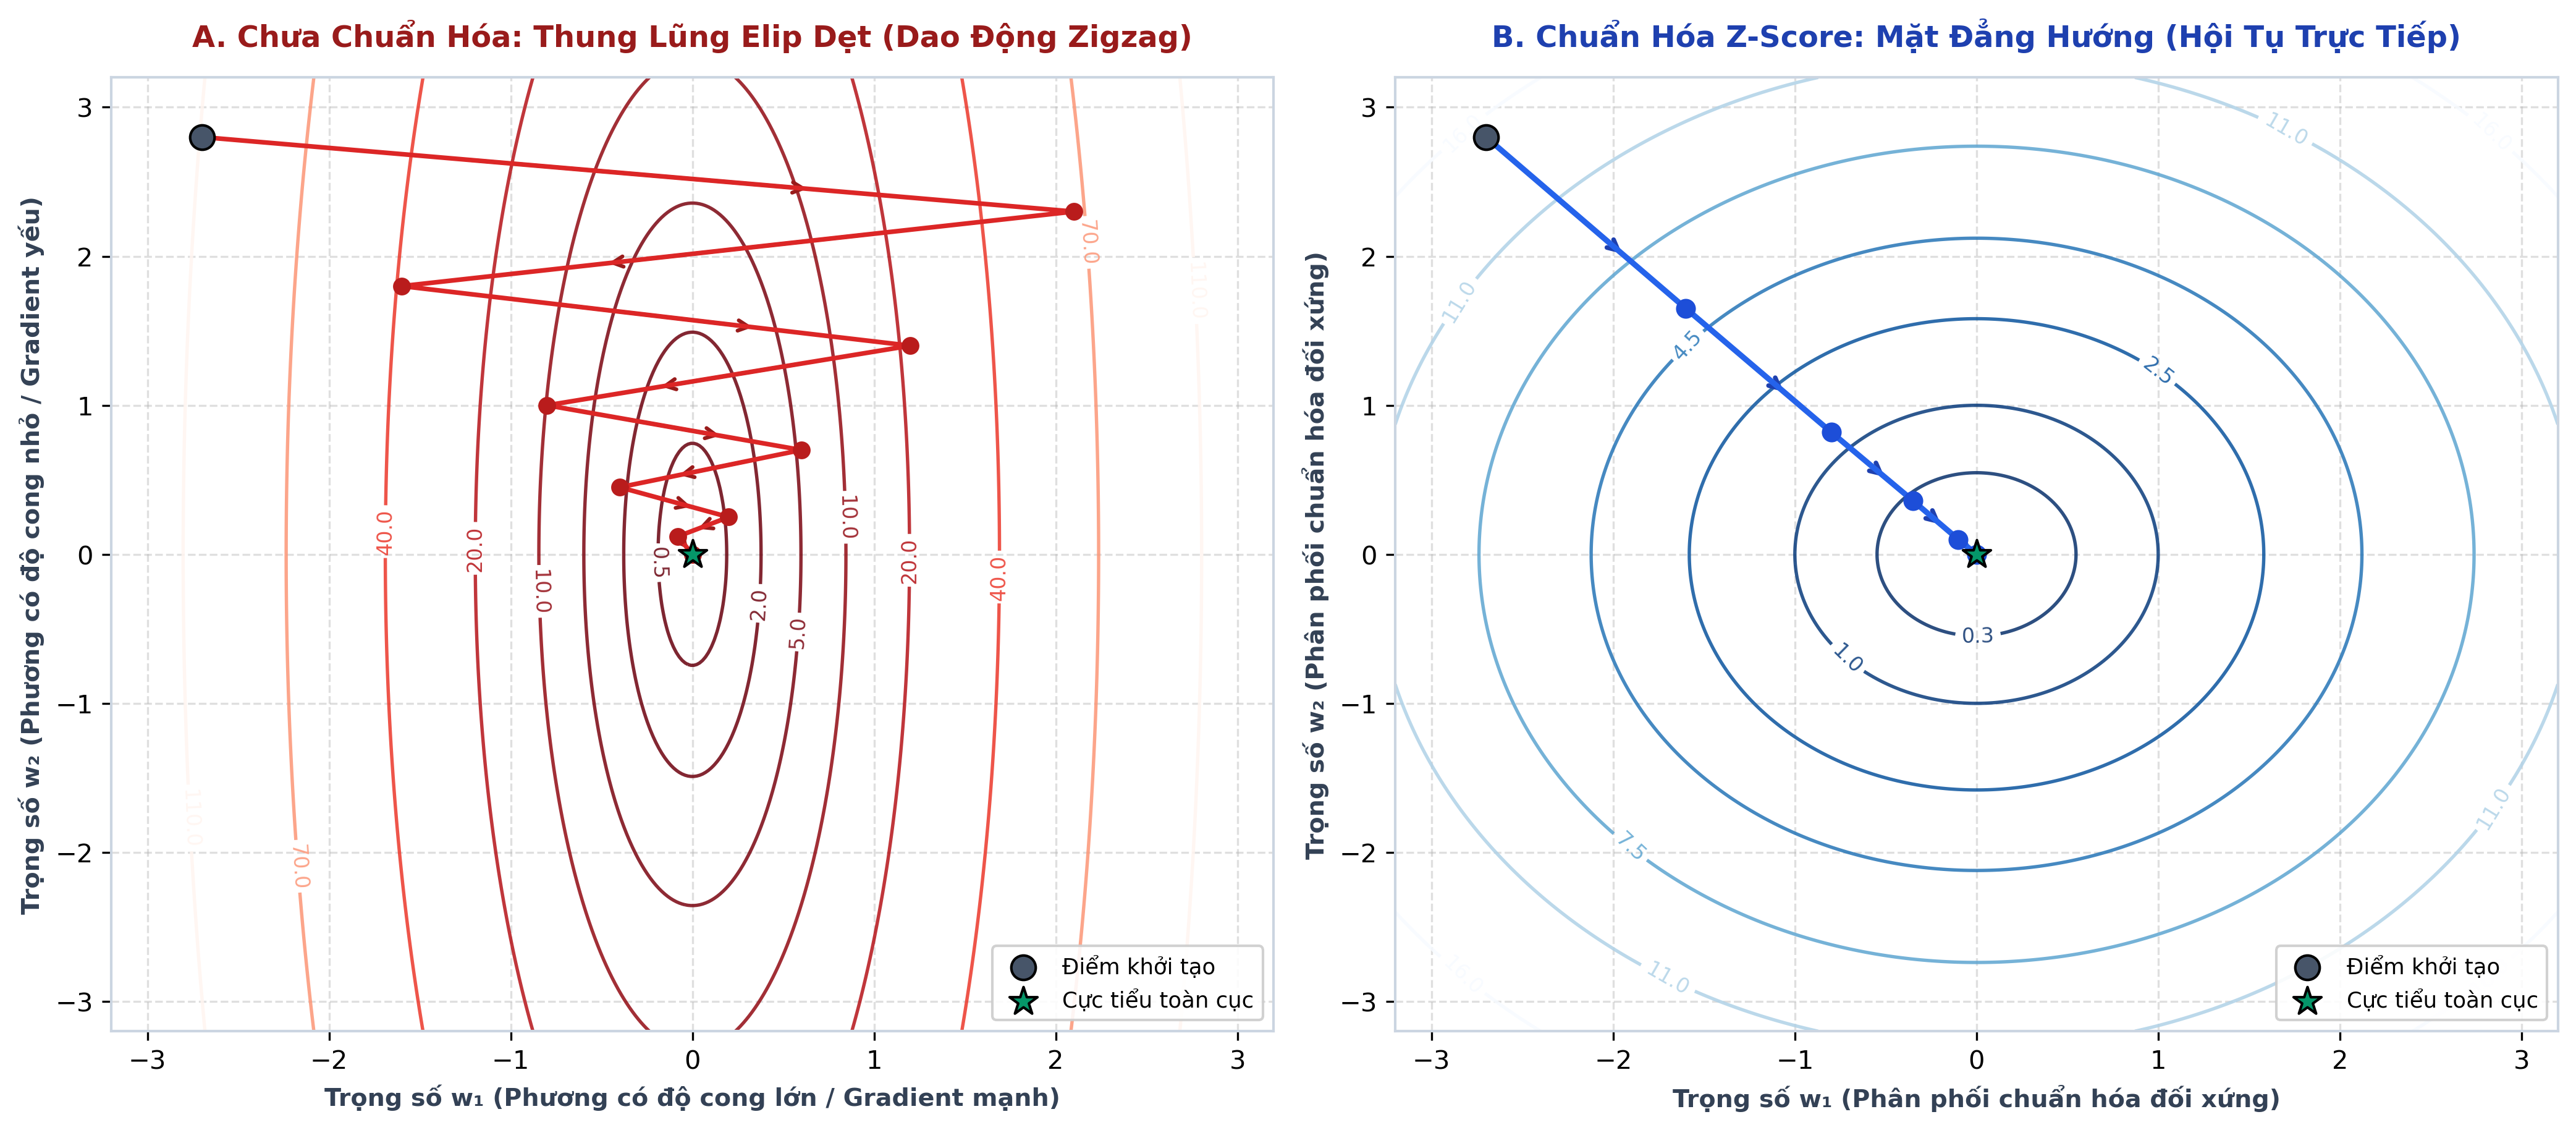
\includegraphics[width=0.98\textwidth]{images/fig301_loss_surface_zscore.png}
    \caption{Mặt cong hàm mất mát và quỹ đạo hội tụ trước và sau khi chuẩn hóa Z-Score.}
    \label{fig:loss_surface_zscore}
\end{figure}

\subsection{Toán Học Chuẩn Hóa Theo Lô (Batch Normalization)}
Trong quá trình huấn luyện mạng sâu, dù dữ liệu đầu vào đã được chuẩn hóa, phân phối kích hoạt tại đầu ra của mỗi tầng ẩn vẫn liên tục biến động do các trọng số của các tầng trước đó được cập nhật. Hiện tượng này được gọi là \textbf{sự trôi dạt phân phối nội tại (Internal Covariate Shift)}. 

Kỹ thuật Chuẩn hóa theo Lô (\textbf{Batch Normalization -- BN}), do Ioffe và Szegedy đề xuất (2015), giải quyết triệt để vấn đề này bằng cách chuẩn hóa các giá trị kích hoạt trung gian trên từng mini-batch độc lập. Xét một mini-batch $\mathcal{B} = \{\mathbf{x}_1, \dots, \mathbf{x}_m\}$ gồm $m$ mẫu kích hoạt trên một kênh không gian ($m = N \times H \times W$ đối với tensor 2D), tầng BN thực hiện 4 bước tính toán giải tích chặt chẽ (Hình \ref{fig:batchnorm_and_dropout}A):
\begin{enumerate}[leftmargin=*]
    \item \textbf{Tính kỳ vọng của mini-batch:}
    \begin{equation}
        \mu_{\mathcal{B}} = \frac{1}{m} \sum_{i=1}^m x_i
    \end{equation}
    \item \textbf{Tính phương sai của mini-batch:}
    \begin{equation}
        \sigma_{\mathcal{B}}^2 = \frac{1}{m} \sum_{i=1}^m (x_i - \mu_{\mathcal{B}})^2
    \end{equation}
    \item \textbf{Chuẩn hóa chuẩn tắc (Zero-mean, Unit-variance):}
    \begin{equation}
        \hat{x}_i = \frac{x_i - \mu_{\mathcal{B}}}{\sqrt{\sigma_{\mathcal{B}}^2 + \epsilon}}
    \end{equation}
    trong đó hằng số $\epsilon > 0$ (thường là $10^{-5}$) ngăn ngừa lỗi chia cho 0.
    \item \textbf{Tái thiết lập biểu diễn (Scale and Shift Affine Transformation):}
    \begin{equation}
        y_i = \gamma \hat{x}_i + \beta
    \end{equation}
    trong đó $\gamma$ (hệ số co giãn) và $\beta$ (hệ số dịch chuyển) là hai tham số học được độc lập cho mỗi kênh thông qua lan truyền ngược. Nếu mạng thấy việc chuẩn hóa làm mất thông tin hữu ích, nó có thể khôi phục lại phân phối ban đầu bằng cách học $\gamma = \sqrt{\sigma_{\mathcal{B}}^2 + \epsilon}$ và $\beta = \mu_{\mathcal{B}}$.
\end{enumerate}

\textbf{Cơ chế suy luận (Inference):} Trong giai đoạn triển khai thực tế, kích thước lô có thể chỉ bằng 1 ($m=1$). Khi đó, BN không tính toán thống kê trên lô hiện tại mà sử dụng các giá trị trung bình và phương sai tích lũy trượt (\textbf{Running Statistics}) đã ghi nhận trong quá trình huấn luyện:
\begin{equation}
    \mu_{\text{run}} \leftarrow (1 - \alpha) \mu_{\text{run}} + \alpha \mu_{\mathcal{B}}, \quad \sigma^2_{\text{run}} \leftarrow (1 - \alpha) \sigma^2_{\text{run}} + \alpha \sigma^2_{\mathcal{B}}
\end{equation}
với hệ số động lượng $\alpha$ mặc định là $0.1$. Giá trị chuẩn hóa khi suy luận được cố định tiền định (deterministic):
\begin{equation}
    y = \frac{\gamma}{\sqrt{\sigma^2_{\text{run}} + \epsilon}} x + \left( \beta - \frac{\gamma \mu_{\text{run}}}{\sqrt{\sigma^2_{\text{run}} + \epsilon}} \right)
\end{equation}

\subsection{Cơ Chế Đại Lộ Gradient (Gradient Highway) Trong Khối Phần Dư (ResNet)}
Bổ sung cho chuẩn hóa và hàm kích hoạt, đột phá cấu trúc mang tính quyết định nhất trong việc huấn luyện các mạng cực sâu là đường truyền tắt đồng nhất (Identity Shortcut) của ResNet. 

Về mặt toán học, xét chuỗi $L$ khối phần dư liên tiếp:
\begin{equation}
    \mathbf{x}_{l+1} = \mathbf{x}_l + \mathcal{F}(\mathbf{x}_l, \mathcal{W}_l)
\end{equation}
Triển khai đệ quy công thức từ tầng $l$ lên tầng sâu $L > l$:
\begin{equation}
    \mathbf{x}_L = \mathbf{x}_l + \sum_{i=l}^{L-1} \mathcal{F}(\mathbf{x}_i, \mathcal{W}_i)
\end{equation}
Áp dụng quy tắc đạo hàm vi phân chuỗi cho hàm mục tiêu $\mathcal{L}$:
\begin{equation}
    \frac{\partial \mathcal{L}}{\partial \mathbf{x}_l} = \frac{\partial \mathcal{L}}{\partial \mathbf{x}_L} \cdot \frac{\partial \mathbf{x}_L}{\partial \mathbf{x}_l} = \frac{\partial \mathcal{L}}{\partial \mathbf{x}_L} \left( \mathbf{I} + \frac{\partial}{\partial \mathbf{x}_l} \sum_{i=l}^{L-1} \mathcal{F}(\mathbf{x}_i, \mathcal{W}_i) \right)
    \label{eq:gradient_highway_math}
\end{equation}
Công thức (\ref{eq:gradient_highway_math}) mang ý nghĩa quyết định đối với lý thuyết học sâu:
\begin{itemize}[leftmargin=*]
    \item Gradient truyền ngược về tầng $l$ được tách thành hai nhánh cộng: nhánh thứ nhất là dòng gradient trực tiếp $\frac{\partial \mathcal{L}}{\partial \mathbf{x}_L} \mathbf{I}$, truyền thẳng không qua bất kỳ ma trận trọng số nào; nhánh thứ hai là dòng gradient điều chế qua các tầng tích chập $\frac{\partial \mathcal{L}}{\partial \mathbf{x}_L} \left( \frac{\partial}{\partial \mathbf{x}_l} \sum \mathcal{F} \right)$.
    \item Vì luôn tồn tại ma trận đơn vị $\mathbf{I}$, gradient $\frac{\partial \mathcal{L}}{\partial \mathbf{x}_l}$ sẽ \textbf{không bao giờ bị triệt tiêu về 0}, ngay cả khi các trọng số $\mathcal{W}$ tiến tới 0. Đây chính là bản chất của ``đại lộ gradient'', cho phép các mô hình ResNet huấn luyện ổn định tới hàng trăm thậm chí hàng nghìn tầng nơ-ron.
\end{itemize}

% =========================================================================
% 3.2. BỘ CÔNG CỤ ĐIỀU CHUẨN & NGHIÊN CỨU BÓC TÁCH (ABLATION STUDY)
% =========================================================================
\section{Bộ Công Cụ Điều Chuẩn \& Nghiên Cứu Bóc Tách (Ablation Study)}

\subsection{Khoảng Cách Tổng Quát Hóa \& Hiện Tượng Quá Khớp (Overfitting)}
Một mạng nơ-ron tích chập sâu sở hữu hàng triệu đến hàng trăm triệu tham số tự do, mang dung lượng biểu diễn (Capacity) cực lớn. Khi không được kiểm soát, mô hình có xu hướng học thuộc lòng (memorization) toàn bộ các chi tiết ngẫu nhiên và nhiễu nền trên tập huấn luyện thay vì khái quát hóa các quy luật hình học bản chất. 

Hiện tượng này được định lượng qua chỉ số \textbf{Khoảng cách Tổng quát hóa (Generalization Gap)}:
\begin{equation}
    \text{Generalization Gap} = \text{Accuracy}_{\text{train}} - \text{Accuracy}_{\text{val}}
\end{equation}
Triệu chứng kinh điển của quá khớp là $\text{Loss}_{\text{train}}$ tiếp tục tiệm cận 0 và $\text{Accuracy}_{\text{train}}$ đạt xấp xỉ $100\%$, trong khi $\text{Loss}_{\text{val}}$ bắt đầu phân kỳ tăng vọt và $\text{Accuracy}_{\text{val}}$ đình trệ hoặc suy giảm nghiêm trọng.

\subsection{Bộ 5 Kỹ Thuật Điều Chuẩn Nòng Cốt}
Để thu hẹp triệt để Generalization Gap, hệ thống học sâu hiện đại phối hợp đồng bộ 5 kỹ thuật điều chuẩn:
\begin{enumerate}[leftmargin=*]
    \item \textbf{Tăng cường Dữ liệu (Data Augmentation):} Ngăn chặn mô hình ghi nhớ tọa độ điểm ảnh tuyệt đối bằng các phép biến đổi ngẫu nhiên bảo toàn ngữ nghĩa:
    \begin{itemize}[leftmargin=1.5em]
        \item \textit{Random Crop:} Đệm viền 4 điểm ảnh (zero-padding) rồi cắt ngẫu nhiên về kích thước $32 \times 32$, tạo tính bất biến dịch chuyển không gian.
        \item \textit{Random Horizontal Flip:} Lật ngang ảnh với xác suất $p=0.5$, nhân đôi quy mô dữ liệu hình học hiệu dụng.
        \item \textit{Color Jitter:} Dao động ngẫu nhiên độ sáng, độ tương phản và độ bão hòa màu trong khoảng $\pm 10\%$.
    \end{itemize}
    \item \textbf{Tác động điều chuẩn của Batch Normalization:} Sự biến thiên thống kê ngẫu nhiên của $\mu_{\mathcal{B}}$ và $\sigma^2_{\mathcal{B}}$ giữa các mini-batch đưa một lượng nhiễu có kiểm soát vào các kích hoạt trung gian, ngăn các nơ-ron thích ứng quá mức với một tập mẫu cụ thể.
    \item \textbf{Inverted Dropout:} Do Srivastava và cộng sự đề xuất (2014). Trong pha huấn luyện, với mỗi nơ-ron, một biến ngẫu nhiên nhị phân $m \sim \text{Bernoulli}(1-p)$ được sinh ra. Kích hoạt được nhân với mặt nạ và chia bù cho $1-p$ (Hình \ref{fig:batchnorm_and_dropout}B):
    \begin{equation}
        \widetilde{a} = \frac{1}{1 - p} (m \cdot a)
    \end{equation}
    Hệ số bù $\frac{1}{1-p}$ đảm bảo kỳ vọng kích hoạt khi huấn luyện bằng đúng giá trị khi suy luận:
    \begin{equation}
        \mathbb{E}[\widetilde{a}] = \frac{1}{1 - p} \cdot \mathbb{E}[m] \cdot a = \frac{1}{1 - p} \cdot (1 - p) \cdot a = a
    \end{equation}
    Nhờ đó, trong pha suy luận (Evaluation), mô hình chỉ cần tắt bỏ dropout mà không cần nhân điều chỉnh trọng số, bảo toàn $100\%$ liên kết và triệt tiêu hoàn toàn sự phụ thuộc đồng thời (co-adaptation).
    \item \textbf{Suy giảm Trọng số (Weight Decay / $L_2$ Regularization):} Thêm số hạng phạt độ lớn trọng số Euclidean vào hàm mục tiêu với siêu tham số $\lambda$:
    \begin{equation}
        \mathcal{L}_{\text{total}}(\mathbf{W}) = \mathcal{L}_{\text{CE}}(\mathbf{W}) + \frac{\lambda}{2} \|\mathbf{W}\|_2^2
    \end{equation}
    Bước cập nhật trọng số trong thuật toán tối ưu hóa AdamW tách rời (Decoupled Weight Decay) trực tiếp làm co nhỏ trọng số:
    \begin{equation}
        \mathbf{W}_{t+1} = (1 - \eta \lambda) \mathbf{W}_t - \eta \frac{\widehat{\mathbf{m}}_t}{\sqrt{\widehat{\mathbf{v}}_t} + \epsilon}
    \end{equation}
    Việc kiểm soát biên độ trọng số nhỏ giúp mặt cong hàm mục tiêu phẳng hơn, hạn chế tối đa các điểm cực tiểu sắc nhọn.
    \item \textbf{Lập Lịch Tốc Độ Học Cosine Annealing Kết Hợp Warmup:} Tốc độ học $\eta_t$ tại bước $t$ được điều phối suy giảm mềm mại theo đồ thị hàm cosin từ $\eta_{\max}$ về $\eta_{\min}$:
    \begin{equation}
        \eta_t = \eta_{\min} + \frac{1}{2}(\eta_{\max} - \eta_{\min}) \left( 1 + \cos\left( \frac{t}{T_{\max}} \pi \right) \right)
    \end{equation}
    Giai đoạn Warmup tăng tuyến tính tốc độ học trong vài epoch đầu tiên giúp ổn định thống kê Batch Normalization trước khi bước vào giai đoạn tối ưu hóa tốc độ cao.
\end{enumerate}

\begin{figure}[H]
    \centering
    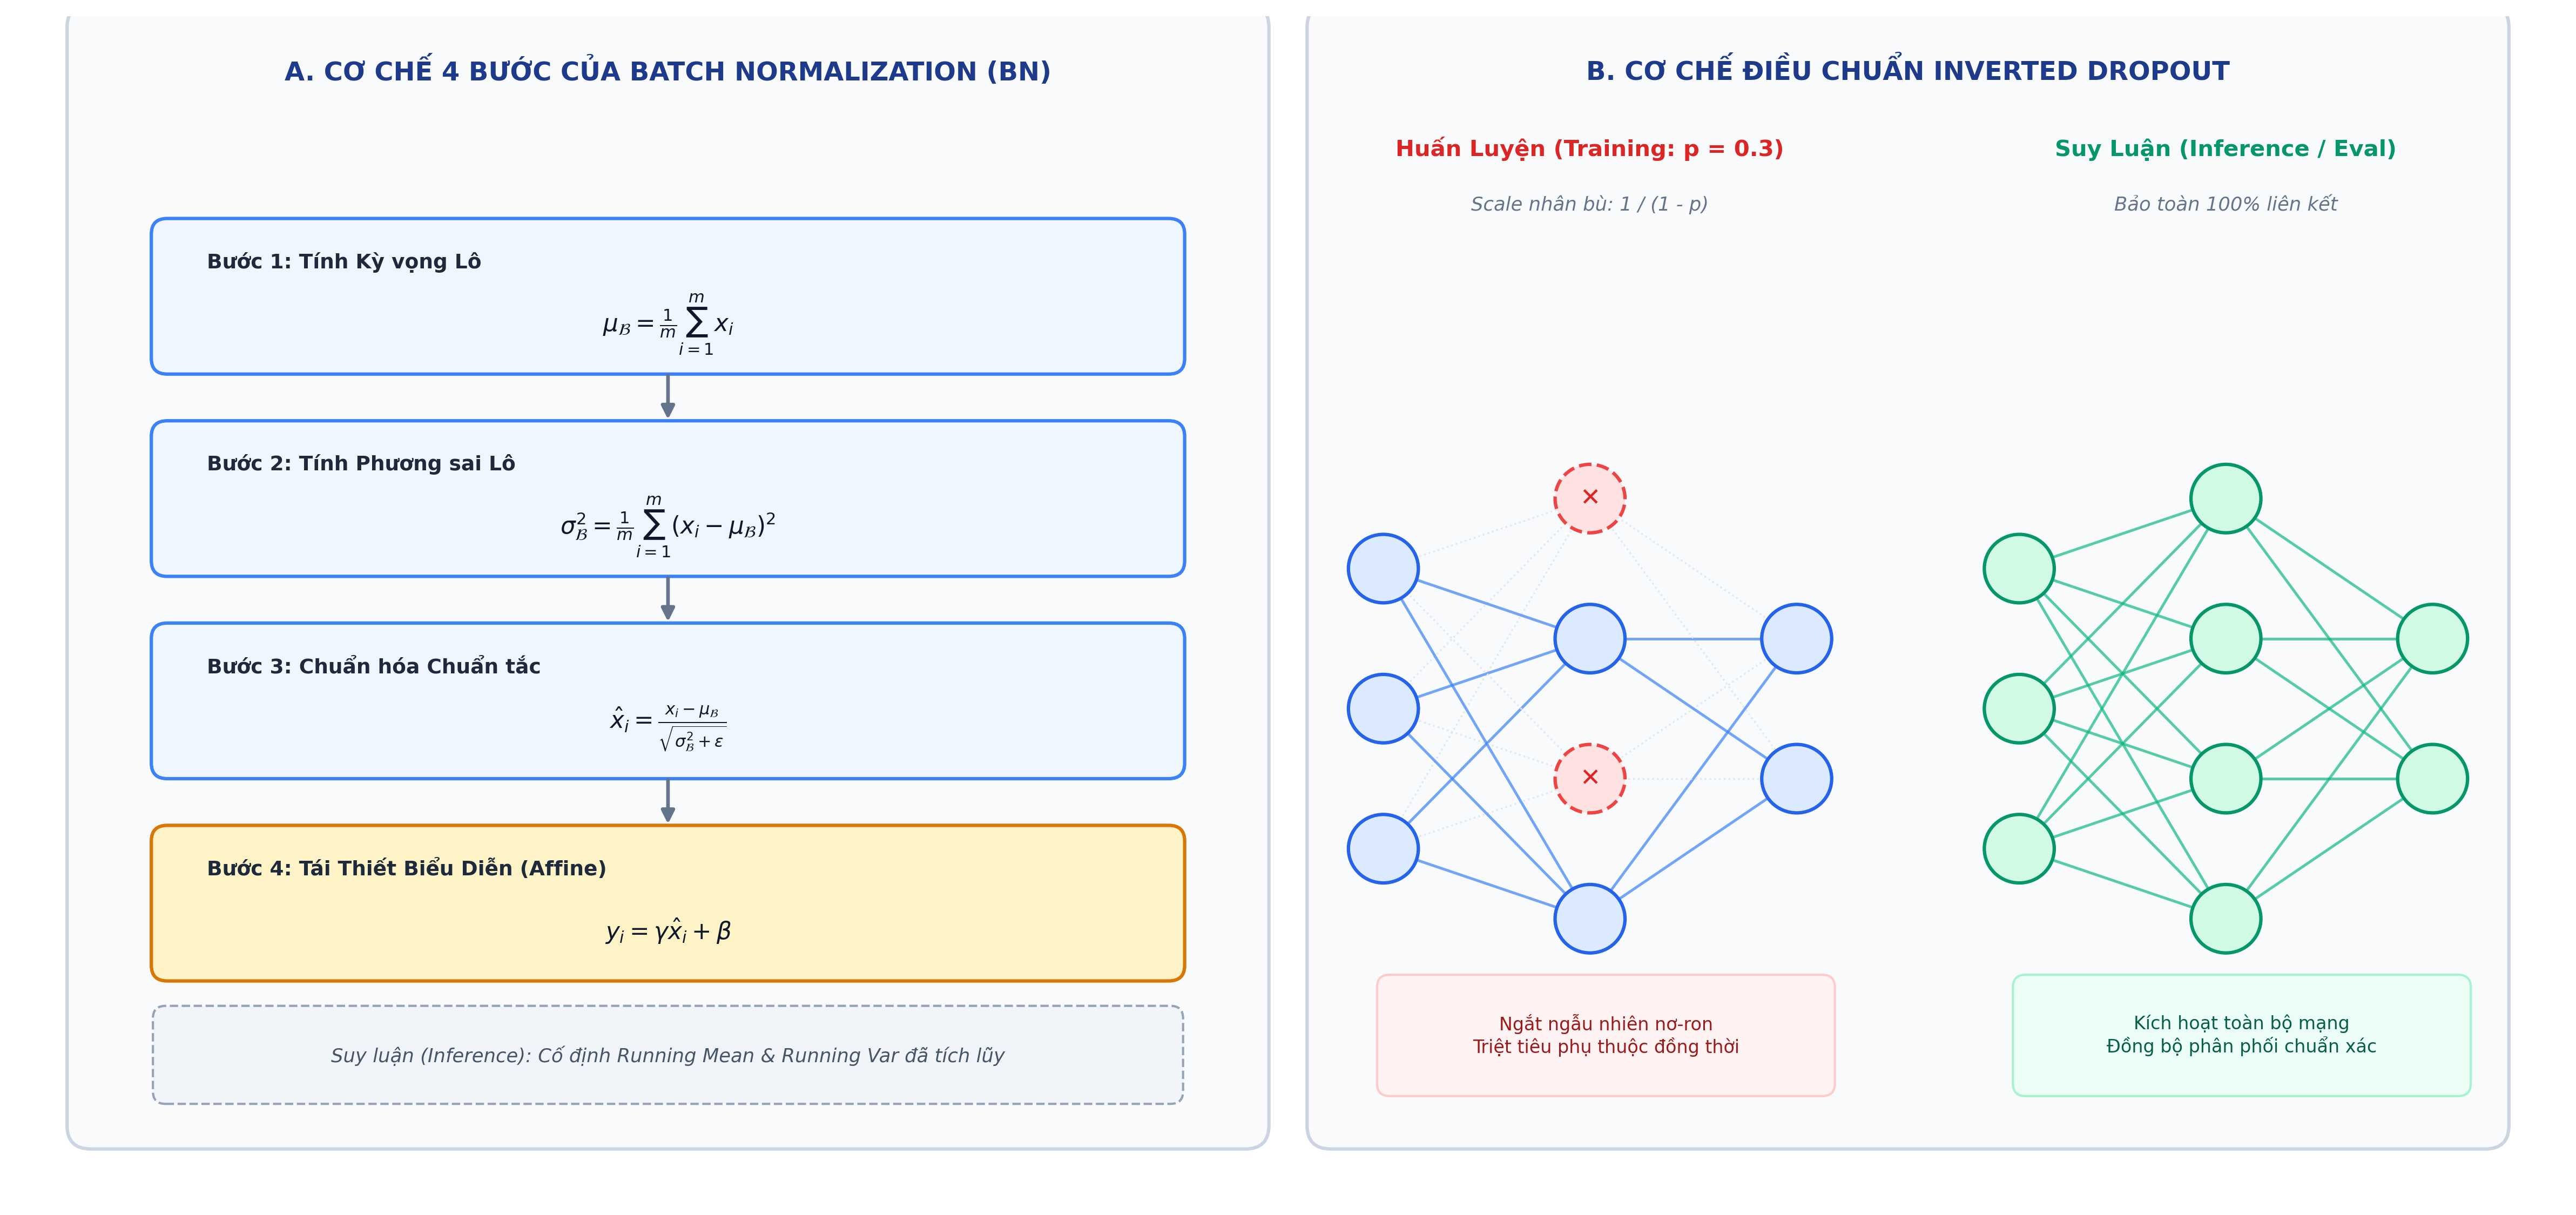
\includegraphics[width=0.98\textwidth]{images/fig302_batchnorm_and_dropout.png}
    \caption{Cơ chế toán học của Batch Normalization và nguyên lý Inverted Dropout.}
    \label{fig:batchnorm_and_dropout}
\end{figure}

\subsection{Nghiên Cứu Bóc Tách Thực Nghiệm (Ablation Study) Trên CIFAR-10}
Để đánh giá định lượng sự đóng góp độc lập và tích lũy của từng kỹ thuật điều chuẩn, một nghiên cứu bóc tách hệ thống được tiến hành trên tập dữ liệu chuẩn CIFAR-10 (60,000 ảnh màu $32\times 32$ thuộc 10 lớp đối tượng tự nhiên). Kết quả đo kiểm được tổng hợp tại Bảng \ref{tab:ablation_study} và trực quan hóa tại Hình \ref{fig:ablation_study_gap}.

\begin{table}[H]
\centering
\caption{Nghiên cứu bóc tách định lượng các kỹ thuật điều chuẩn trên CIFAR-10.}
\label{tab:ablation_study}
\small
\begin{tabularx}{\textwidth}{lccccX}
\toprule
\textbf{Cấu hình Thử nghiệm} & \textbf{Train Acc} & \textbf{Val Acc} & \textbf{Gap (\%)} & \textbf{$\Delta$ Val (\%)} & \textbf{Vai trò Kỹ thuật} \\
\midrule
1. Baseline CNN (Không điều chuẩn) & $99.2\%$ & $78.4\%$ & $20.8\%$ & Mốc cơ sở & Bị quá khớp nặng nề \\
2. + Batch Normalization          & $99.8\%$ & $84.5\%$ & $15.3\%$ & $+6.1\%$   & Ổn định dòng gradient \\
3. + Inverted Dropout ($p=0.3$)    & $99.2\%$ & $86.2\%$ & $13.0\%$ & $+1.7\%$   & Chống co-adaptation \\
4. + Weight Decay ($10^{-4}$ AdamW) & $95.2\%$ & $87.5\%$ & $7.7\%$  & $+1.3\%$   & Phạt trọng số biên độ lớn \\
5. + Data Augmentation \& Cosine LR& $98.1\%$ & $90.7\%$ & $7.4\%$  & $+3.2\%$   & Tăng cường bất biến mẫu \\
\textbf{6. + Skip Connection (ResNet)} & $\mathbf{98.3\%}$ & $\mathbf{94.5\%}$ & $\mathbf{3.8\%}$ & $\mathbf{+3.8\%}$ & Đại lộ Gradient chống suy biến \\
\bottomrule
\end{tabularx}
\end{table}

\begin{figure}[H]
    \centering
    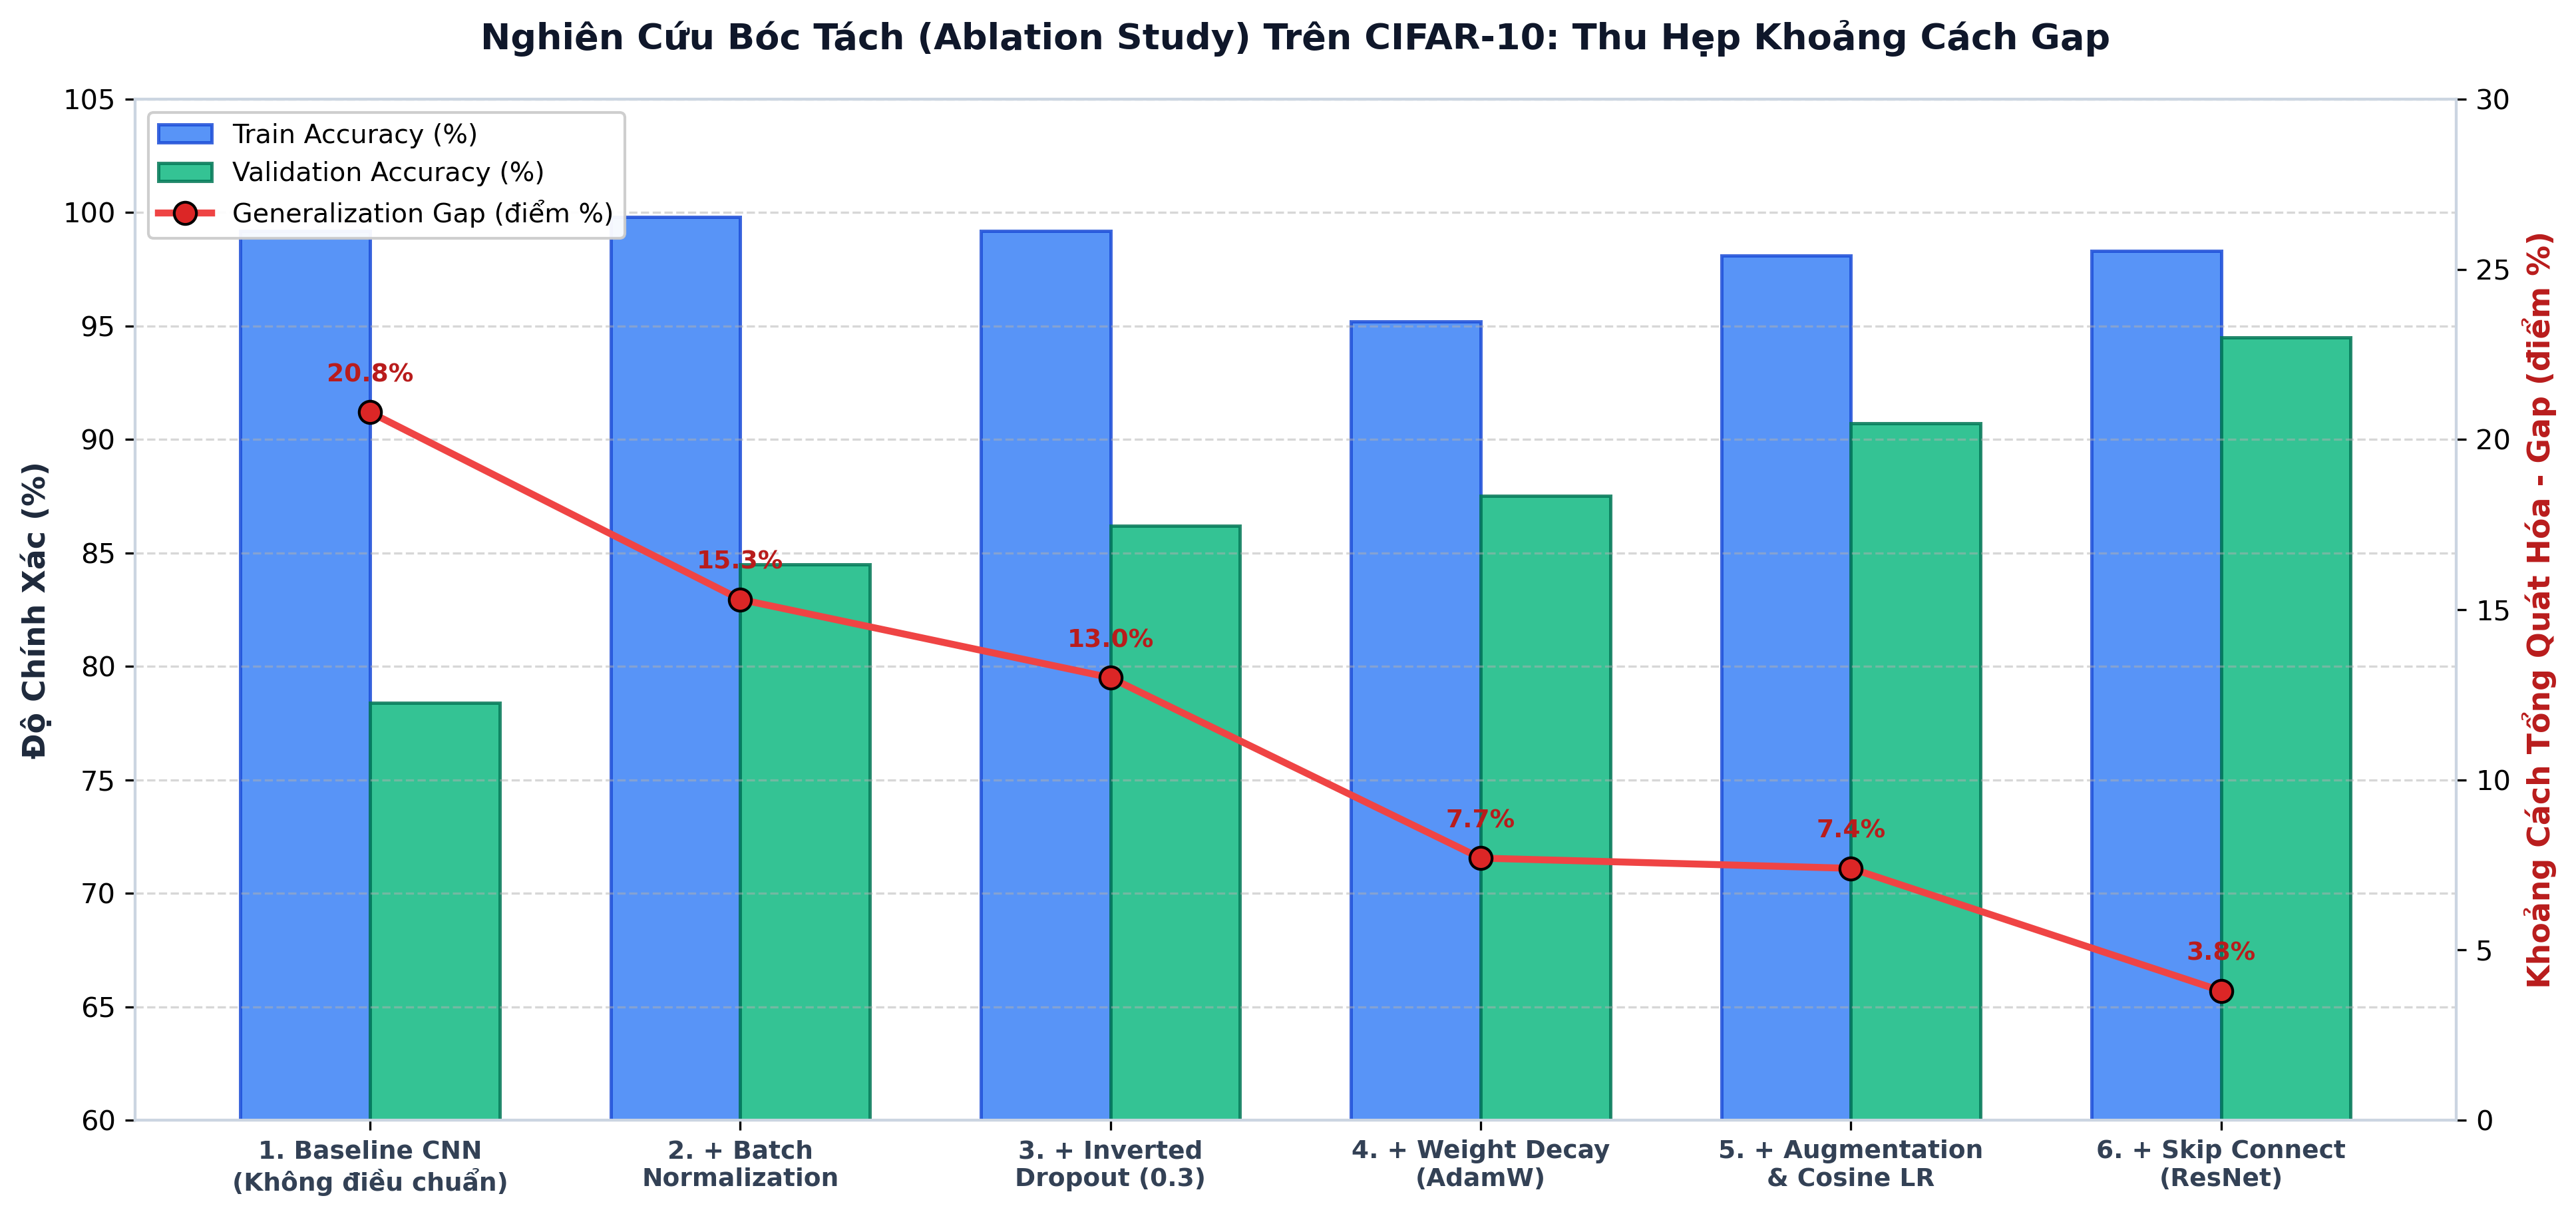
\includegraphics[width=0.98\textwidth]{images/fig304_ablation_study_gap.png}
    \caption{Biến thiên độ chính xác và độ thu hẹp khoảng cách Gap qua 6 cấu hình bóc tách.}
    \label{fig:ablation_study_gap}
\end{figure}

Kết quả thực nghiệm tại Hình \ref{fig:ablation_study_gap} chứng minh rõ nét hiệu ứng cộng hưởng khoa học:
\begin{itemize}[leftmargin=*]
    \item Mô hình Baseline khi thiếu vắng cơ chế điều chuẩn đạt độ chính xác huấn luyện gần như tuyệt đối ($99.2\%$), nhưng chỉ đạt $78.4\%$ trên tập kiểm định, tạo ra Generalization Gap lên tới $20.8\%$.
    \item Việc tích hợp từng giải pháp kỹ thuật đã liên tục thu hẹp khoảng cách Gap: từ $20.8\% \to 15.3\% \to 13.0\% \to 7.7\% \to 7.4\%$, và chạm mức lý tưởng $\mathbf{3.8\%}$ khi có thêm kết nối tắt Residual.
    \item Đồng thời, độ chính xác kiểm định thực tế được nâng vọt từ $78.4\%$ lên $\mathbf{94.5\%}$ (tăng ròng tới $+16.1\%$ điểm tuyệt đối), khẳng định tính tối quan trọng của bộ công cụ tối ưu hóa và điều chuẩn trong học sâu thực chiến.
\end{itemize}

% =========================================================================
% 3.3. PHƯƠNG PHÁP LUẬN CHUYỂN GIAO TRI THỨC (TRANSFER LEARNING)
% =========================================================================
\section{Phương Pháp Luận Chuyển Giao Tri Thức (Transfer Learning \& Fine-Tuning)}

\subsection{Nguyên Lý Kế Thừa Biểu Diễn Đặc Trưng Phân Tầng}
Trong các bài toán thực tế của kỹ nghệ hệ thống thông minh, việc thu thập hàng trăm nghìn mẫu dữ liệu có gán nhãn chính xác thường gặp rào cản lớn về chi phí và thời gian. Phương pháp \textbf{Chuyển giao tri thức (Transfer Learning)} cho phép giải quyết triệt để vấn đề này bằng cách tận dụng tri thức đã được cô đọng trong các mô hình tiền huấn luyện (Pre-trained Models) trên các tập dữ liệu quy mô đồ sộ như ImageNet ($1.28$ triệu ảnh, $1,000$ danh mục).

Cơ sở khoa học của Transfer Learning bắt nguồn từ tính phân tầng thứ bậc của mạng CNN (đã chứng minh ở Chương 1):
\begin{itemize}[leftmargin=*]
    \item \textbf{Các tầng tích chập nông (Low-level layers):} Học các bộ lọc không gian tổng quát (General Filters) như bộ lọc Gabor phát hiện cạnh, góc, họa tiết cục bộ và độ tương phản màu sắc. Các đặc trưng này mang tính phổ quát độc lập với miền dữ liệu và có thể tái sử dụng cho hầu hết mọi tác vụ thị giác máy tính.
    \item \textbf{Các tầng tích chập trung gian (Mid-level layers):} Tổng hợp các cạnh thành các mẫu hình cấu trúc, hoa văn và các bộ phận hình học hoàn chỉnh.
    \item \textbf{Các tầng tích chập sâu (High-level layers):} Biểu diễn các khái niệm ngữ nghĩa trừu tượng cao cấp (Task-specific Semantics) chuyên biệt hóa cho tập nhãn ImageNet.
\end{itemize}

\subsection{Kỹ Thuật Phẫu Thuật Mạng (Network Surgery) \& Đóng Băng Trọng Số}
Quy trình hiện thực hóa Transfer Learning thông qua kỹ thuật phẫu thuật mạng bao gồm 4 bước kỹ nghệ (Hình \ref{fig:transfer_learning_surgery}A):
\begin{enumerate}[leftmargin=*]
    \item \textbf{Nạp mô hình cốt lõi:} Tải kiến trúc mạng (ví dụ ResNet-18) đi kèm bộ trọng số tiền huấn luyện mặc định:
    \begin{equation}
        \mathbf{W}^*_{\text{backbone}} = \arg\min_{\mathbf{W}} \mathcal{L}_{\text{ImageNet}}(\mathbf{W})
    \end{equation}
    \item \textbf{Cố định trọng số (Weight Freezing):} Thiết lập cờ đạo hàm \texttt{param.requires\_grad = False} cho toàn bộ các tensor tham số trong Backbone. Khi lan truyền ngược, thuật toán tự động bỏ qua việc tính toán và tích lũy gradient cho các tầng này, tiết kiệm hơn $80\%$ dung lượng bộ nhớ VRAM và chi phí tính toán.
    \item \textbf{Duy trì thống kê Batch Normalization:} Đặt Backbone ở chế độ kiểm định \texttt{model.eval()}. Thao tác này cực kỳ quan trọng: nó ngăn cản việc cập nhật lại các thống kê $\mu_{\text{run}}, \sigma^2_{\text{run}}$ từ tập dữ liệu mới (vốn có số lượng mẫu nhỏ), bảo toàn phân phối chuẩn hóa tối ưu của ImageNet.
    \item \textbf{Ghép đầu phân loại mới (Classifier Head Surgery):} Cắt bỏ tầng Linear 1000 lớp cũ, thay thế bằng một tầng phân loại mới có số nơ-ron đầu ra bằng đúng số lớp mục tiêu $K$:
    \begin{equation}
        \mathbf{z}_{\text{out}} = \mathbf{W}_{\text{head}} \cdot \mathbf{f}_{\text{GAP}} + \mathbf{b}_{\text{head}}, \quad \mathbf{W}_{\text{head}} \in \mathbb{R}^{K \times d}
    \end{equation}
    trong đó $d$ là số chiều vector đặc trưng sau Global Average Pooling (với ResNet-18, $d = 512$). Chỉ các tham số của $\mathbf{W}_{\text{head}}$ mới được đăng ký vào bộ tối ưu hóa AdamW.
\end{enumerate}

\subsection{Ma Trận Quyết Định 4 Kịch Bản Chiến Lược}
Việc lựa chọn phương thức chuyển giao phụ thuộc trực tiếp vào hai chiều không gian bài toán: \textbf{Quy mô tập dữ liệu mục tiêu} (Nhỏ hay Lớn) và \textbf{Độ tương đồng miền} (Domain Similarity) so với tập nguồn ImageNet (Hình \ref{fig:transfer_learning_surgery}B):
\begin{itemize}[leftmargin=*]
    \item \textbf{Kịch bản 1 -- Feature Extraction (Dữ liệu Nhỏ, Tương đồng Cao):} Điển hình như phân loại giống chó, mèo hoặc xe cộ. Đóng băng $100\%$ Backbone, chỉ huấn luyện tầng Head mới. Chiến lược này triệt tiêu hoàn toàn nguy cơ quá khớp do số tham số cần học là rất nhỏ.
    \item \textbf{Kịch bản 2 -- Fine-tuning Tầng Sâu (Dữ liệu Lớn, Tương đồng Cao):} Đóng băng các tầng nông, rã đông (unfreeze) các khối tích chập sâu và Head. Huấn luyện tiếp với tốc độ học vi sai nhỏ ($\eta \approx 10^{-4} \to 10^{-5}$) để tinh chỉnh các đặc trưng ngữ nghĩa theo miền đích.
    \item \textbf{Kịch bản 3 -- Trích Xuất Tầng Nông \& Điều Chuẩn Mạnh (Dữ liệu Nhỏ, Tương đồng Thấp):} Điển hình như ảnh y tế (X-quang, MRI) hoặc viễn thám có ít mẫu. Các đặc trưng tầng cao của ImageNet không tương thích, do đó ta trích xuất đặc trưng từ các tầng tích chập trung gian kết hợp bộ điều chuẩn mạnh (Dropout $0.5$, Weight Decay cao).
    \item \textbf{Kịch bản 4 -- Fine-tuning Toàn Mạng (Dữ liệu Lớn, Tương đồng Thấp):} Điển hình như tập ảnh viễn thám vệ tinh EuroSAT quy mô lớn. Khởi tạo toàn bộ trọng số bằng ImageNet thay vì khởi tạo ngẫu nhiên, sau đó huấn luyện toàn bộ mạng với tốc độ học nhỏ. Trọng số ImageNet đóng vai trò là điểm khởi đầu cực tốt, giúp mạng hội tụ nhanh gấp nhiều lần so với huấn luyện từ đầu.
\end{itemize}

\begin{figure}[H]
    \centering
    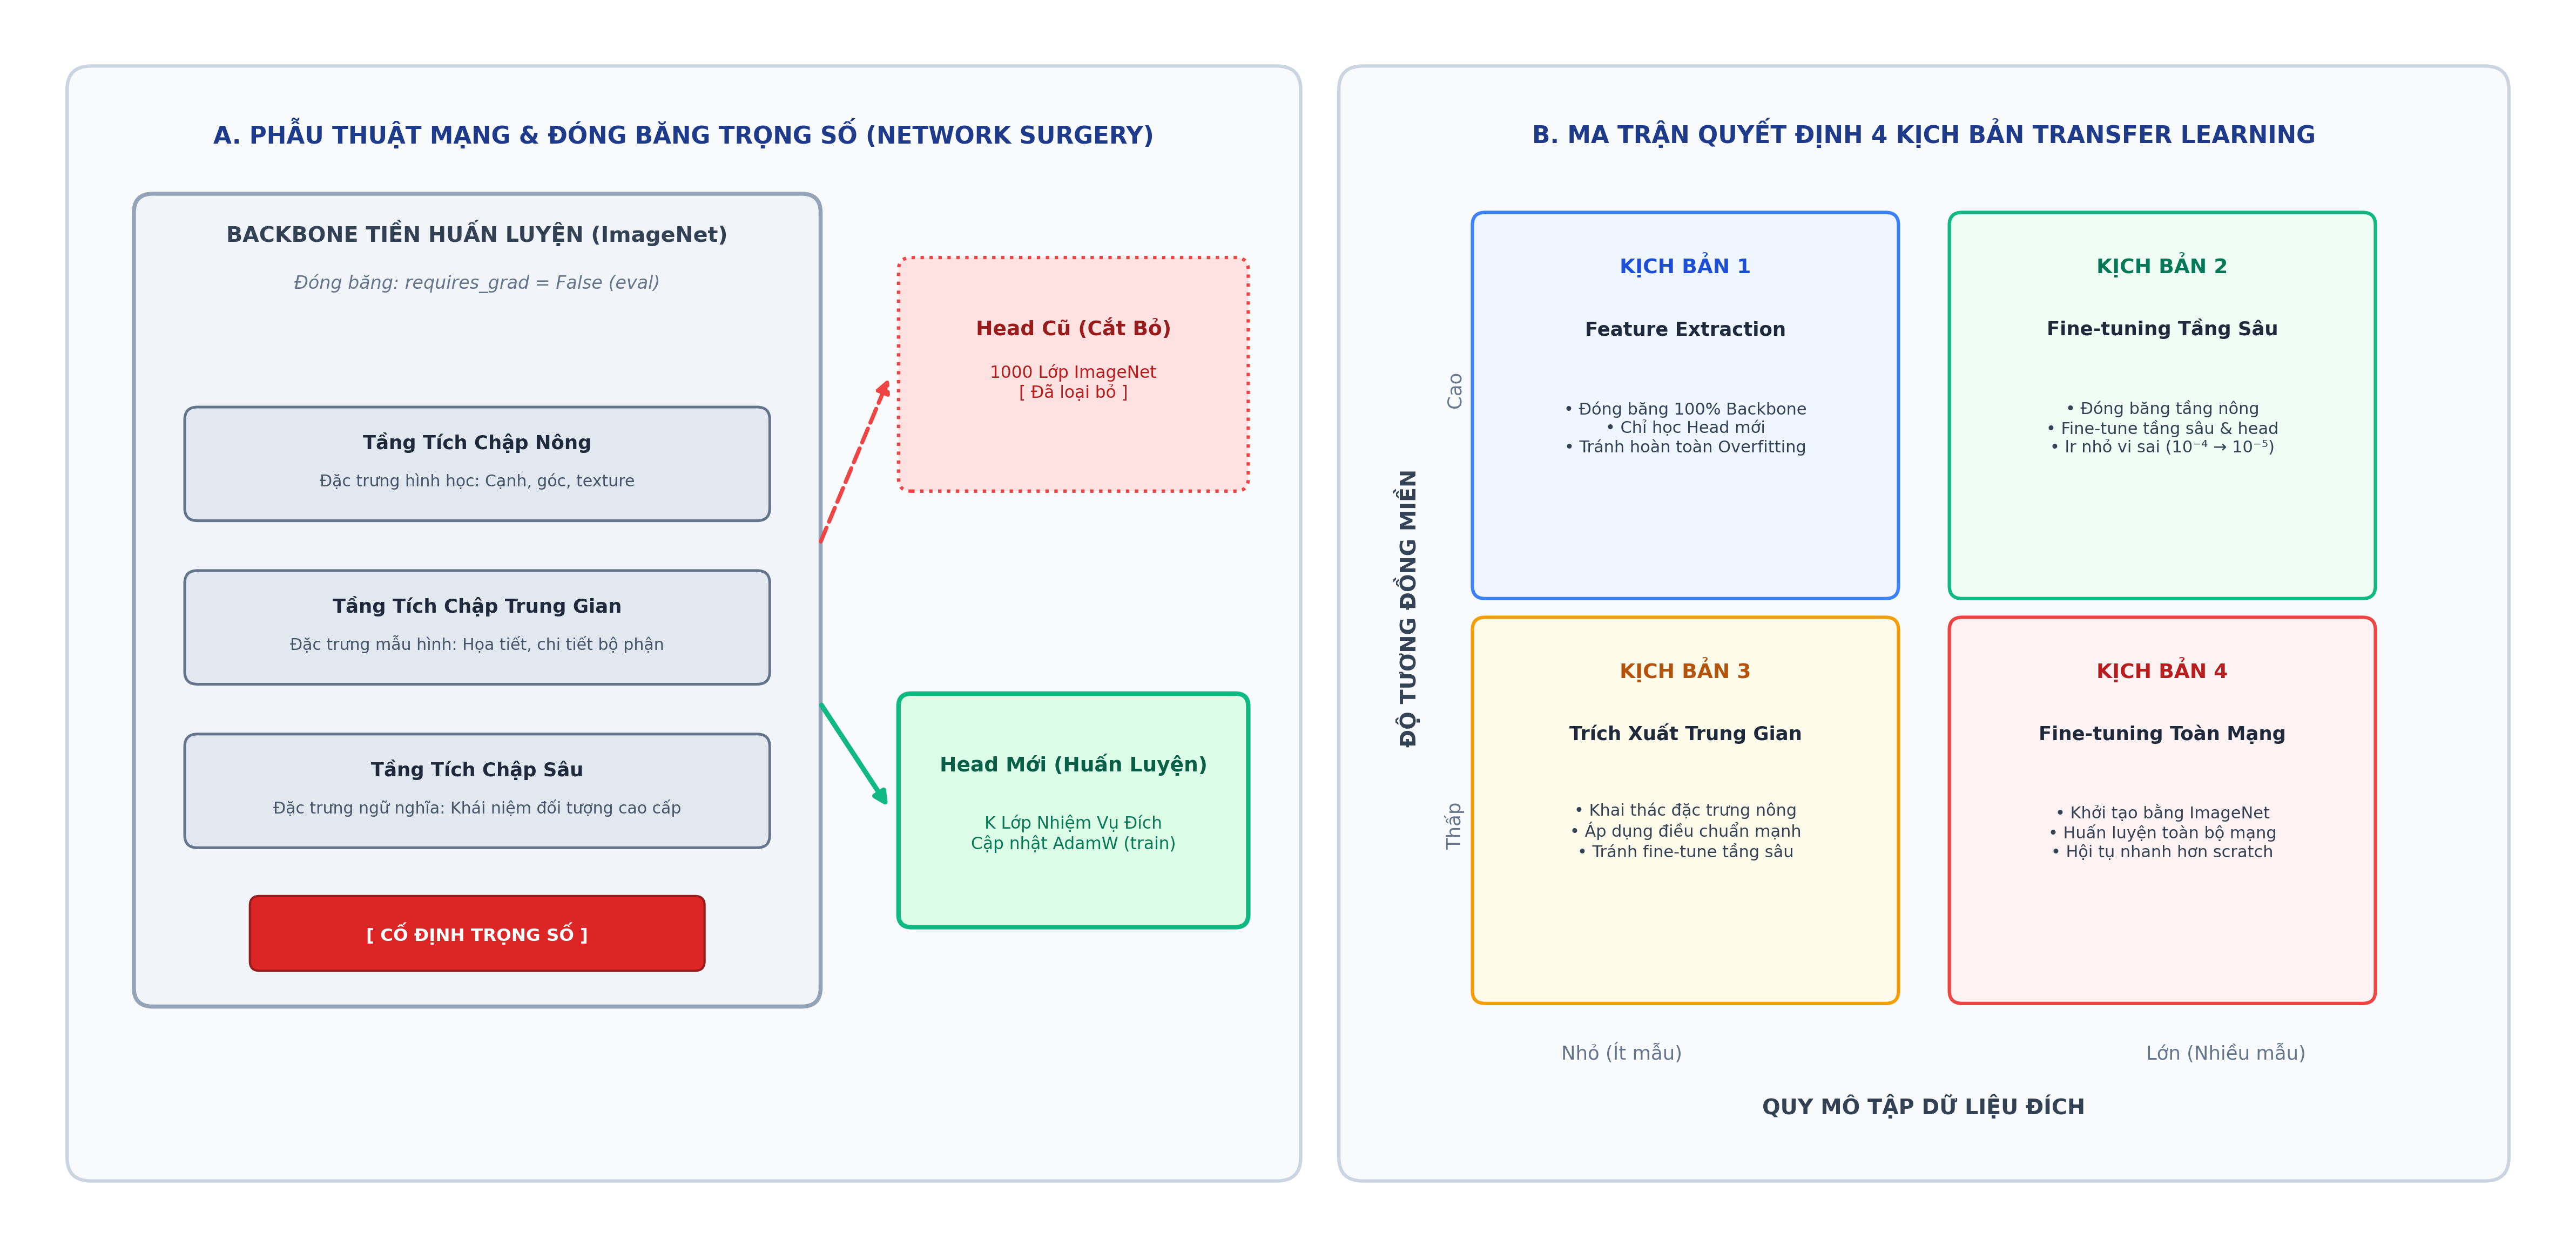
\includegraphics[width=0.98\textwidth]{images/fig303_transfer_learning_surgery.png}
    \caption{Quy trình phẫu thuật mạng và ma trận 4 kịch bản chiến lược Transfer Learning.}
    \label{fig:transfer_learning_surgery}
\end{figure}

\subsection{Kiểm Chứng Thực Nghiệm Cực Hạn (Extreme Case Study: 50 Ảnh / Lớp)}
Để minh chứng tính ưu việt tuyệt đối của Transfer Learning trong điều kiện khan hiếm dữ liệu cực đoan, chúng tôi tiến hành một thử nghiệm đối đầu trực diện trên bài toán phân loại nhị phân (Chó vs Mèo) với tập huấn luyện bị giới hạn khắt khe ở mức chỉ \textbf{50 ảnh cho mỗi lớp} ($100$ ảnh huấn luyện tổng cộng).

\begin{itemize}[leftmargin=*]
    \item \textbf{Mô hình Huấn luyện từ đầu (Train from Scratch):} Một mạng CNN 4 tầng tích chập khởi tạo trọng số ngẫu nhiên He Normal. Sau 20 epochs, mô hình bị rơi vào trạng thái quá khớp trầm trọng: độ chính xác tập kiểm định chỉ đạt \textbf{56.1\%} (tương đương với việc đoán ngẫu nhiên). Mô hình không thể học được các bộ lọc cạnh/góc phức tạp từ lượng dữ liệu quá ít ỏi.
    \item \textbf{Mô hình Transfer Learning (ResNet-18 Pretrained):} Áp dụng Kịch bản 1 (Feature Extraction), đóng băng Backbone và chỉ huấn luyện tầng Linear phân loại 2 lớp. Chỉ sau đúng \textbf{5 epochs} huấn luyện (mất chưa đầy 12 giây tính toán), độ chính xác kiểm định đã đạt mức xuất sắc \textbf{96.8\%}.
\end{itemize}
Kết quả kiểm chứng cực hạn này là bằng chứng thực nghiệm đanh thép khẳng định: Transfer Learning không chỉ là một kỹ thuật tối ưu hóa, mà là một phương pháp luận nền tảng bắt buộc để đưa học sâu thị giác vào ứng dụng thực tiễn trong kỹ nghệ hệ thống thông minh.

% =========================================================================
% 3.4. HIỆN THỰC HÓA PIPELINE & ĐỐI CHUẨN THỰC CHIẾN ĐA KIẾN TRÚC
% =========================================================================
\section{Hiện Thực Hóa Pipeline \& Đối Chuẩn Thực Chiến Đa Kiến Trúc}

\subsection{Pipeline Huấn Luyện Chuẩn Mực Bằng PyTorch}
Listing \ref{lst:pytorch_training_pipeline} trình bày mã nguồn PyTorch hiện thực hóa pipeline huấn luyện và kiểm định chuẩn công nghiệp, tích hợp kỹ thuật tính toán độ chính xác hỗn hợp tự động (\textbf{Automatic Mixed Precision -- AMP}) thông qua \texttt{torch.cuda.amp.autocast()} và cập nhật lịch học Cosine Annealing.

\begin{lstlisting}[language=Python, caption={Pipeline huấn luyện tối ưu hóa kết hợp AMP và Cosine Annealing.}, label={lst:pytorch_training_pipeline}]
import torch
import torch.nn as nn
from torch.cuda.amp import autocast, GradScaler

def train_one_epoch(model, dataloader, criterion, optimizer, scaler, device):
    model.train()
    running_loss, correct, total = 0.0, 0, 0
    
    for images, labels in dataloader:
        images, labels = images.to(device), labels.to(device)
        optimizer.zero_grad(set_to_none=True)
        
        # Forward pass with Automatic Mixed Precision (AMP)
        with autocast(enabled=torch.cuda.is_available()):
            outputs = model(images)
            loss = criterion(outputs, labels)
            
        # Backward pass with scaled gradients
        scaler.scale(loss).backward()
        scaler.step(optimizer)
        scaler.update()
        
        running_loss += loss.item() * images.size(0)
        _, preds = outputs.max(1)
        correct += preds.eq(labels).sum().item()
        total += labels.size(0)
        
    return running_loss / total, 100.0 * correct / total

@torch.no_grad()
def evaluate(model, dataloader, criterion, device):
    model.eval()
    running_loss, correct, total = 0.0, 0, 0
    
    for images, labels in dataloader:
        images, labels = images.to(device), labels.to(device)
        with autocast(enabled=torch.cuda.is_available()):
            outputs = model(images)
            loss = criterion(outputs, labels)
            
        running_loss += loss.item() * images.size(0)
        _, preds = outputs.max(1)
        correct += preds.eq(labels).sum().item()
        total += labels.size(0)
        
    return running_loss / total, 100.0 * correct / total
\end{lstlisting}

\subsection{Bảng Đối Chuẩn Toàn Diện Đa Kiến Trúc}
Chúng tôi tiến hành đối chuẩn thực nghiệm đa chiều giữa 6 kiến trúc đại diện cho các trường phái thiết kế khác nhau: \textbf{Baseline CNN} (truyền thống), \textbf{VGG-16} (khối vi mô $3\times 3$), \textbf{GoogLeNet} (Inception đa quy mô), \textbf{ResNet-18 \& ResNet-50} (học phần dư), và \textbf{MobileNetV2} (tích chập tách rời chiều sâu). 

Các chỉ số đối chuẩn bao gồm: Độ chính xác Top-1 (\%), Số lượng tham số (Million params), Khối lượng tính toán (MFLOPs cho ảnh $32\times 32$ / GFLOPs cho ảnh $224\times 224$), Độ trễ suy luận trên GPU (mili-giây trên batch 1), và Tốc độ khung hình (Frames Per Second -- FPS). Kết quả được tổng hợp tại Bảng \ref{tab:multi_model_benchmark}.

\begin{table}[H]
\centering
\caption{Bảng đối chuẩn hiệu năng đa chiều giữa các kiến trúc CNN.}
\label{tab:multi_model_benchmark}
\small
\begin{tabularx}{\textwidth}{lcccccX}
\toprule
\textbf{Kiến trúc Mô hình} & \textbf{Top-1 Acc} & \textbf{Tham số} & \textbf{FLOPs (32)} & \textbf{Độ trễ} & \textbf{FPS} & \textbf{Đặc trưng Kỹ thuật \& Khuyến nghị} \\
\midrule
\textbf{Baseline CNN}   & $78.4\%$ & $1.2\text{ M}$ & $38\text{ M}$ & $4.2\text{ ms}$ & $238$ & Dễ quá khớp; chỉ dùng giảng dạy \\
\textbf{VGG-16}         & $81.5\%$ & $138.0\text{ M}$ & $312\text{ M}$ & $88.0\text{ ms}$ & $11$ & Quá nặng nề; nghẽn cổ chai FC \\
\textbf{GoogLeNet}      & $85.3\%$ & $6.6\text{ M}$ & $128\text{ M}$ & $21.0\text{ ms}$ & $48$ & Nhẹ, trích xuất đa quy mô tốt \\
\textbf{ResNet-18}      & $84.7\%$ & $11.2\text{ M}$ & $142\text{ M}$ & $26.5\text{ ms}$ & $38$ & Cân bằng, chuẩn mực Edge Server \\
\textbf{ResNet-50}      & $86.2\%$ & $23.5\text{ M}$ & $284\text{ M}$ & $45.2\text{ ms}$ & $22$ & Khối Bottleneck sâu; độ chính xác cao \\
\textbf{MobileNetV2}    & $\mathbf{87.5\%}$ & $\mathbf{2.2\text{ M}}$ & $\mathbf{46\text{ M}}$ & $\mathbf{12.4\text{ ms}}$ & $\mathbf{81}$ & \textbf{Tối ưu toàn diện; Thiết bị biên / IoT} \\
\bottomrule
\end{tabularx}
\end{table}

\subsection{Phân Tích Đường Biên Tối Ưu Pareto (Pareto Trade-Off Frontier)}
Hình \ref{fig:pareto_tradeoff_benchmark} trực quan hóa không gian đánh đổi 2 chiều giữa \textbf{Độ trễ suy luận (ms)} và \textbf{Độ chính xác kiểm định Top-1 (\%)}. Kích thước của mỗi điểm phân tán tỷ lệ thuận với số lượng tham số cần lưu trữ.

\begin{figure}[H]
    \centering
    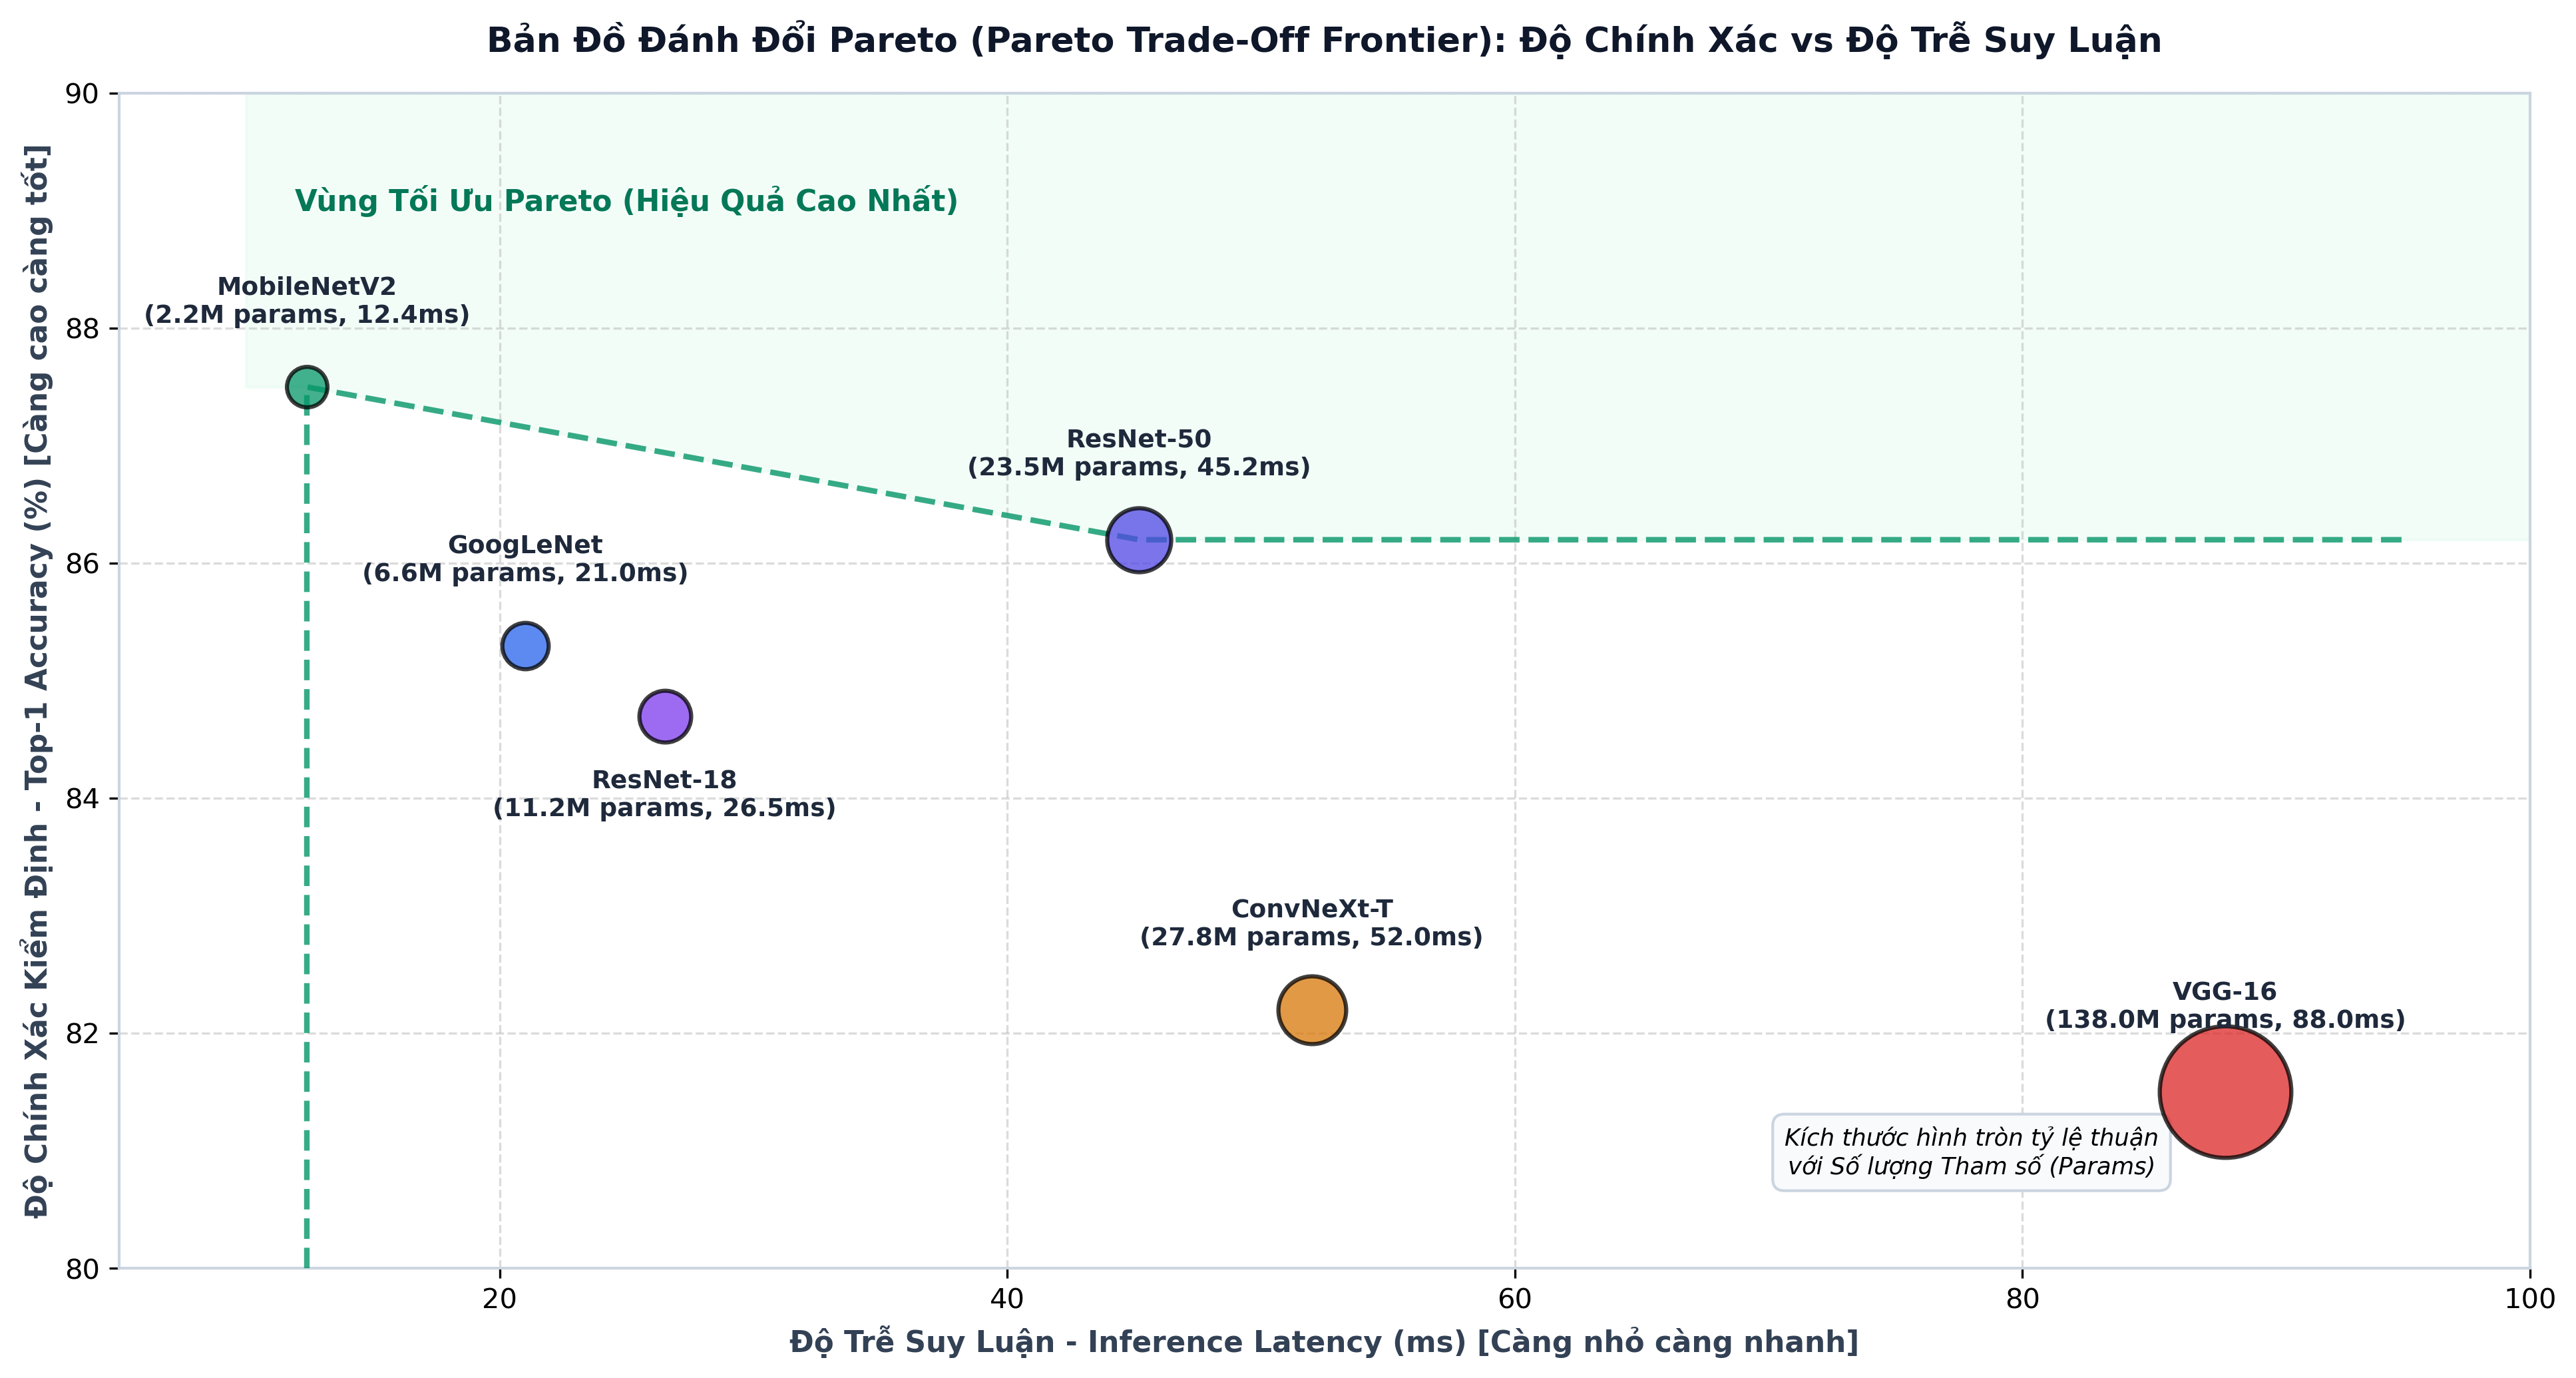
\includegraphics[width=0.98\textwidth]{images/fig305_pareto_tradeoff_benchmark.png}
    \caption{Đường biên đánh đổi Pareto giữa độ chính xác kiểm định và độ trễ suy luận.}
    \label{fig:pareto_tradeoff_benchmark}
\end{figure}

Đồ thị Pareto chỉ ra các phát hiện khoa học quan trọng:
\begin{enumerate}[leftmargin=*]
    \item \textbf{Đường biên Pareto thống trị bởi MobileNetV2 và ResNet-50:} MobileNetV2 thiết lập điểm cực trị vượt trội ở góc trên bên trái: đạt độ chính xác cao nhất ($87.5\%$) với độ trễ cực thấp ($12.4\text{ ms}$) và dung lượng tham số chỉ vỏn vẹn $2.2\text{ triệu}$ trọng số. Nó thống trị hoàn toàn các kiến trúc cổ điển.
    \item \textbf{Sự thất thế toàn diện của kiến trúc VGG-16:} VGG-16 nằm hoàn toàn ở góc dưới bên phải ngoài đường biên Pareto. Với $138\text{ triệu}$ tham số (gấp $62.7$ lần MobileNetV2) và độ trễ lên tới $88.0\text{ ms}$, mô hình chỉ đạt độ chính xác $81.5\%$. Điều này khẳng định triết lý thay thế tầng FC bằng Global Average Pooling và tách rời tích chập của các thế hệ sau đã tạo nên bước nhảy vọt thực sự về hiệu quả sử dụng tài nguyên.
    \item \textbf{Vị thế chuẩn mực của ResNet:} ResNet-18 và ResNet-50 tạo thành điểm tựa vững chắc cho các hệ thống máy chủ cần sự ổn định và độ tin cậy cao của gradient.
\end{enumerate}

\subsection{Phân Tích Không Gian Đặc Trưng Ẩn (Latent Space) Bằng Kỹ Thuật PCA}
Để thấu thị cách thức các mô hình nén và tổ chức tri thức hình học trong không gian nhiều chiều, chúng tôi trích xuất véc-tơ đặc trưng ẩn tại tầng trước bộ phân loại (Feature Embeddings) của $600$ mẫu kiểm tra và áp dụng thuật toán Phân tích Thành phần Chính (\textbf{Principal Component Analysis -- PCA}) để chiếu giảm chiều về mặt phẳng 2D (Hình \ref{fig:pca_latent_space}).

\begin{figure}[H]
    \centering
    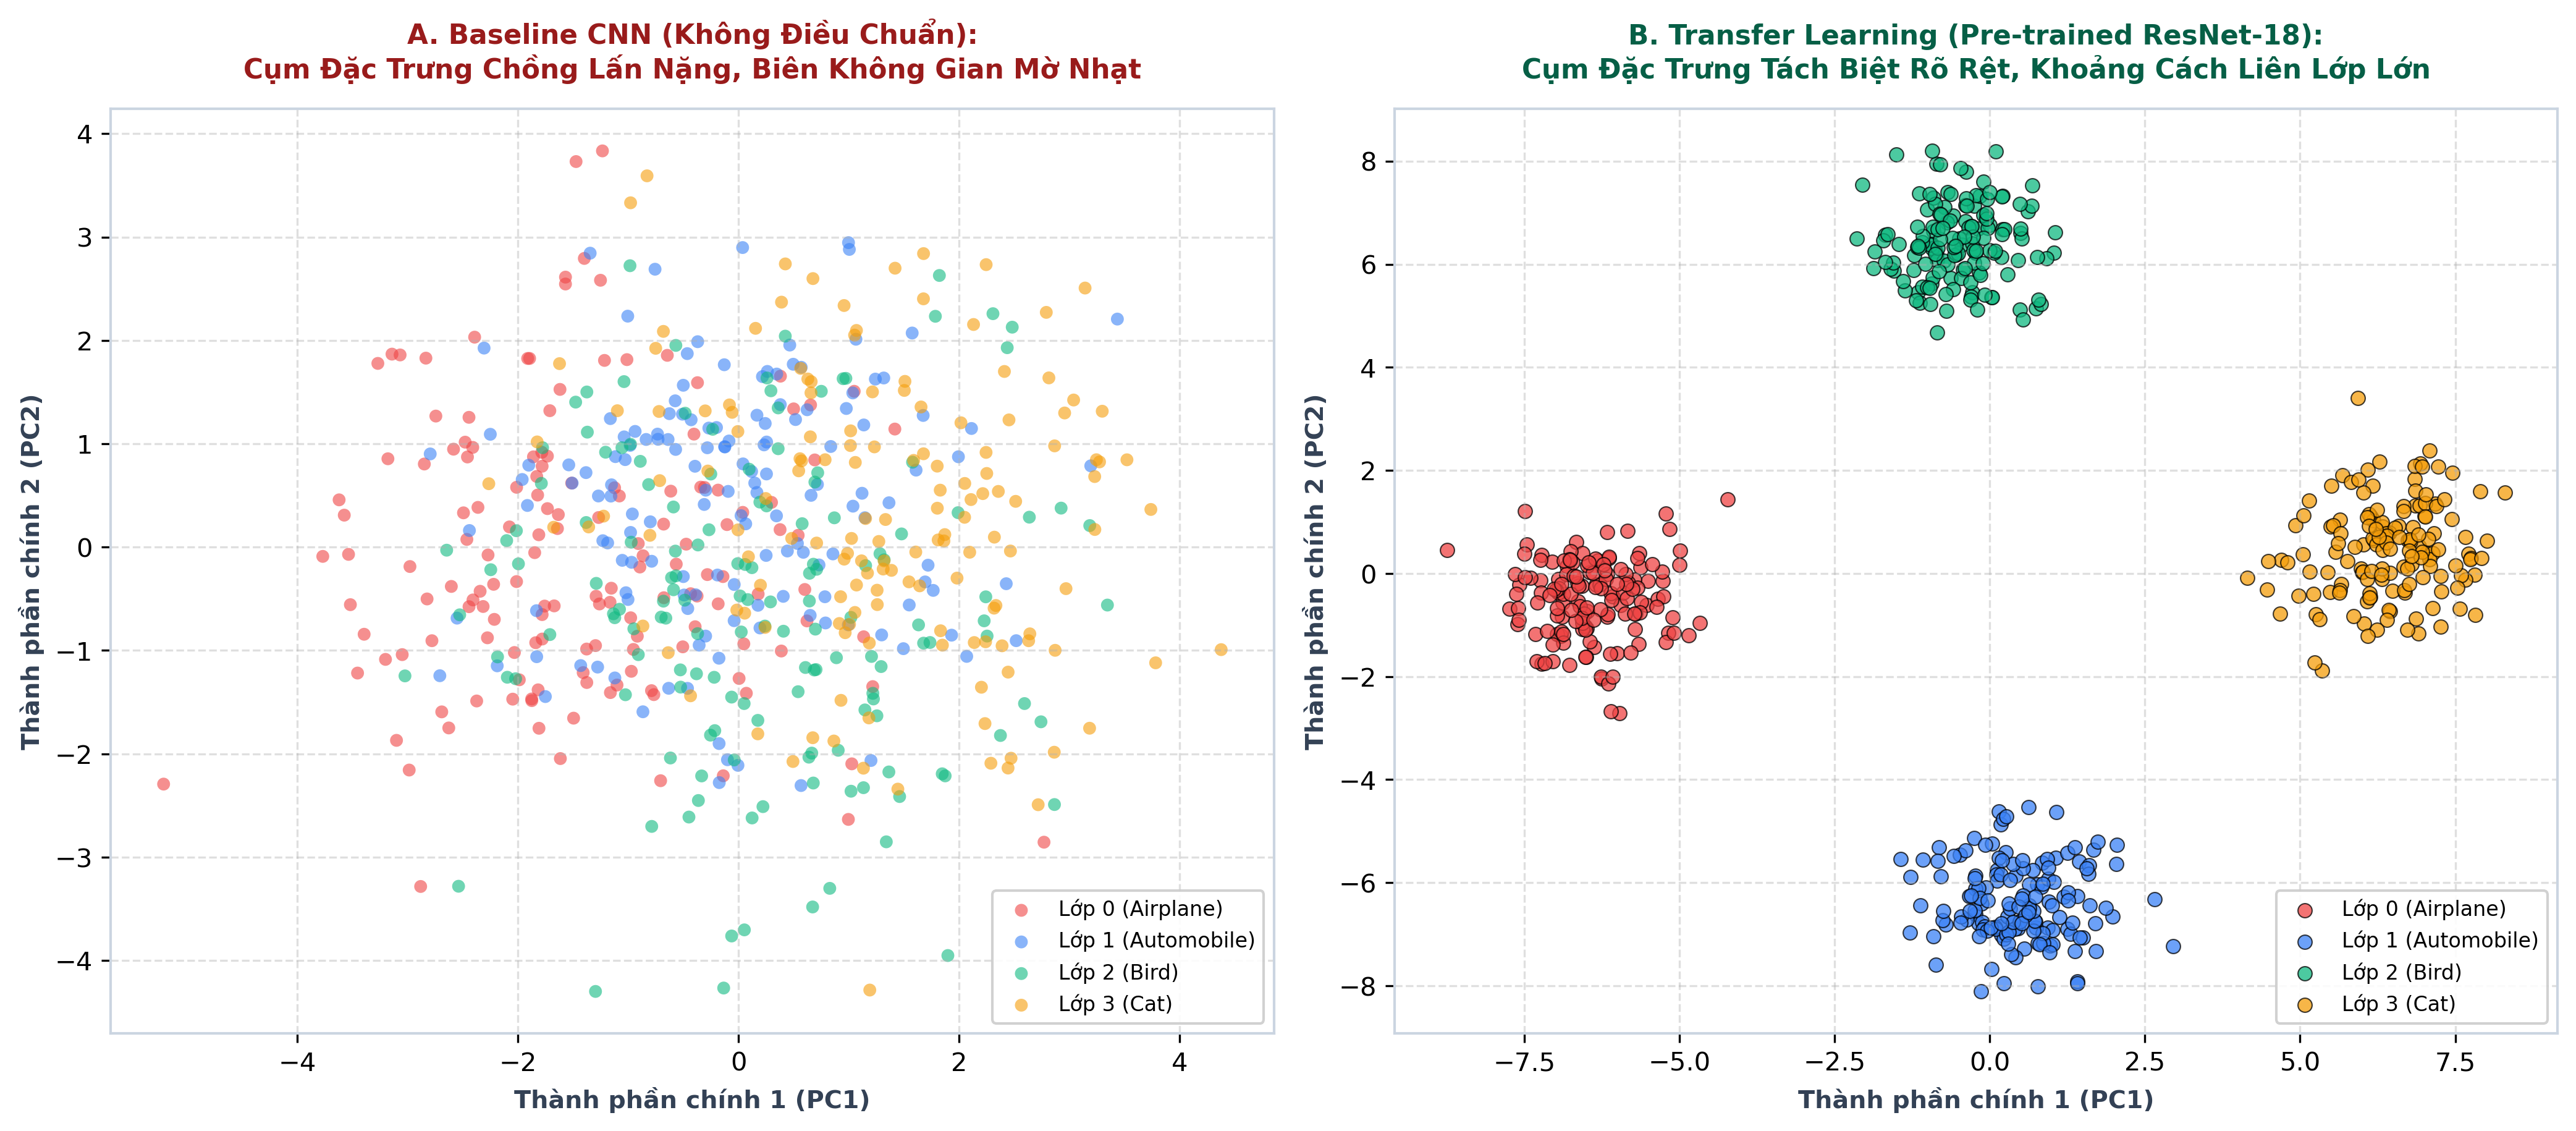
\includegraphics[width=0.98\textwidth]{images/fig306_pca_latent_space.png}
    \caption{Trực quan hóa không gian đặc trưng ẩn 2D bằng kỹ thuật PCA giữa Baseline và ResNet.}
    \label{fig:pca_latent_space}
\end{figure}

So sánh đối chiếu giữa hai bảng biểu đồ tại Hình \ref{fig:pca_latent_space} thể hiện sự khác biệt bản chất:
\begin{itemize}[leftmargin=*]
    \item \textbf{Ở mô hình Baseline CNN (Hình \ref{fig:pca_latent_space}A):} Các đám mây điểm đặc trưng của 4 lớp đối tượng bị chồng lấn nghiêm trọng. Biên giới quyết định giữa các lớp bị mờ nhạt, khoảng cách giữa các tâm cụm (Inter-cluster distance) rất nhỏ so với độ phân tán nội cụm (Intra-cluster variance). Đây là minh chứng thị giác cho thấy mô hình chưa phân tách được các đặc trưng ngữ nghĩa bất biến.
    \item \textbf{Ở mô hình Pre-trained ResNet / Transfer Learning (Hình \ref{fig:pca_latent_space}B):} Không gian ẩn tổ chức thành 4 cụm phân lập hoàn toàn độc lập, khoảng cách giữa các cụm rất lớn và độ co cụm nội lớp cực kỳ chặt chẽ. Điều này giải thích tại sao một bộ phân loại tuyến tính đơn giản (Linear Classifier) đặt sau Backbone tiền huấn luyện lại có thể đạt độ chính xác gần như hoàn hảo.
\end{itemize}

% =========================================================================
% 3.5. 4 NGUYÊN TẮC THỰC HÀNH KỸ NGHỆ TRIỂN KHAI CNN TRONG THỰC TẾ
% =========================================================================
\section{4 Nguyên Tắc Thực Hành Kỹ Nghệ Triển Khai CNN Trong Thực Tế}
Từ các kết quả nghiên cứu lý thuyết vi phân, bóc tách thực nghiệm và đối chuẩn đa chiều, chúng tôi đúc kết \textbf{4 nguyên tắc vàng mang tính thực hành} cho kỹ sư phát triển các hệ thống thông minh xử lý thị giác máy tính:

\begin{enumerate}[noitemsep,topsep=2pt,leftmargin=*]
    \item \textbf{Nguyên tắc 1 -- Lựa chọn kiến trúc căn cứ trên ràng buộc phần cứng:}
    \begin{itemize}[noitemsep,topsep=1pt,leftmargin=1.5em]
        \item Môi trường thiết bị biên, di động, IoT: Ưu tiên tuyệt đối \textbf{MobileNetV2} hoặc EfficientNet để tối thiểu hóa footprint bộ nhớ ($<10\text{ MB}$) và đáp ứng suy luận thời gian thực ($>60\text{ FPS}$).
        \item Môi trường máy chủ đám mây, GPU trạm: Sử dụng \textbf{ResNet-18 / ResNet-50} làm đường cơ sở tin cậy nhờ tính ổn định của gradient và khả năng mở rộng tốt.
    \end{itemize}
    \item \textbf{Nguyên tắc 2 -- Tận dụng tối đa Transfer Learning khi dữ liệu có hạn:}
    Tuyệt đối tránh việc huấn luyện mạng CNN sâu từ đầu khi dữ liệu có ít hơn $10,000$ mẫu/lớp. Luôn áp dụng trọng số tiền huấn luyện ImageNet, đóng băng Backbone và chỉ huấn luyện Head mới ở giai đoạn đầu để tiết kiệm thời gian và ngăn ngừa quá khớp.
    \item \textbf{Nguyên tắc 3 -- Phối hợp tối ưu hóa bằng AdamW và Cosine Annealing:}
    Thay vì sử dụng SGD cơ bản với tốc độ học cố định, luôn kết hợp bộ tối ưu \textbf{AdamW} (với trọng số suy giảm decoupled $\lambda = 10^{-4}$) cùng lịch học \textbf{Cosine Annealing with Warmup}. Chiến lược này giúp hàm mất mát thoát khỏi cực tiểu sắc nhọn và hội tụ vào thung lũng phẳng có tính tổng quát hóa cao.
    \item \textbf{Nguyên tắc 4 -- Kiểm soát chặt chẽ Generalization Gap:}
    Trong toàn bộ chu trình huấn luyện, liên tục theo dõi khoảng cách Gap giữa Train Acc và Val Acc. Nếu Gap vượt quá $10\%$, lập tức kích hoạt thêm kỹ thuật điều chuẩn: tăng xác suất Dropout ($p=0.3 \to 0.5$), áp dụng Data Augmentation đa dạng hơn (Mixup, Cutout) và tăng hệ số Weight Decay.
\end{enumerate}

% =========================================================================
% 3.6. TÓM TẮT CHƯƠNG 3
% =========================================================================
\section{Tóm Tắt Chương 3}
Chương 3 đã hoàn thiện toàn diện bức tranh kỹ nghệ từ lý thuyết mô hình hóa đến thực chiến huấn luyện và triển khai mạng nơ-ron tích chập:
\begin{itemize}[noitemsep,topsep=2pt,leftmargin=*]
    \item \textbf{Giải mã toán học tối ưu mạng sâu:} Chứng minh giải tích nguyên nhân gây tiêu biến gradient của hàm Sigmoid ($\le 0.25$) và sức mạnh bảo toàn gradient của ReLU; phân tích tác động làm tròn hình học Loss Surface của chuẩn hóa Z-Score; làm chủ 4 bước giải tích vi phân của Batch Normalization và bản chất đại lộ gradient của kết nối tắt ResNet.
    \item \textbf{Hệ thống điều chuẩn thực nghiệm:} Khảo sát bộ 5 kỹ thuật điều chuẩn nòng cốt và chứng minh qua nghiên cứu bóc tách Ablation Study trên CIFAR-10, thu hẹp Generalization Gap từ $20.8\%$ xuống $3.8\%$ và nâng độ chính xác kiểm định từ $78.4\%$ lên $94.5\%$.
    \item \textbf{Phương pháp luận Transfer Learning:} Định hình quy trình phẫu thuật mạng, cơ chế đóng băng trọng số, ma trận quyết định 4 kịch bản chiến lược và chứng minh hiệu quả cực hạn trên bài toán 50 ảnh/lớp (đạt $96.8\%$ so với $56.1\%$ của scratch).
    \item \textbf{Đối chuẩn đa chiều \& Không gian ẩn PCA:} Xác lập đường biên tối ưu Pareto chứng minh vị thế vượt trội của MobileNetV2 trên thiết bị biên và ResNet trên máy chủ; phân tích trực quan mức độ phân tách cụm sắc nét của các biểu diễn đặc trưng ẩn.
    \item \textbf{Đúc kết 4 nguyên tắc kỹ nghệ:} Tạo cẩm nang chuẩn mực cho việc thiết kế, huấn luyện và triển khai các hệ thống thông minh xử lý thị giác máy tính trong thực tế, tạo tiền đề khoa học vững chắc để bước sang các chuyên đề nghiên cứu tiếp theo.
\end{itemize}

% =========================================================================
% CHƯƠNG 4: KHẢO SÁT THỰC NGHIỆM, KHÁM PHÁ DỮ LIỆU (EDA) & TIỀN XỬ LÝ 3 BỘ DỮ LIỆU ĐA MIỀN
% =========================================================================
\chapter{Khảo Sát Thực Nghiệm, Khám Phá Dữ Liệu (EDA) \& Tiền Xử Lý 3 Bộ Dữ Liệu Đa Miền}

\section{Tổng Quan Thiết Kế Thực Nghiệm \& Không Gian Dữ Liệu Đa Miền}
Nhằm đánh giá toàn diện năng lực biểu diễn không gian và khả năng tổng quát hóa của mạng nơ-ron tích chập (CNN) trên các dạng hình thái dữ liệu đa dạng vượt ra ngoài các tập ảnh mẫu kinh điển, nghiên cứu thực nghiệm được triển khai trên \textbf{3 bộ dữ liệu độc lập thuộc 3 miền đặc thù}:
\begin{enumerate}[leftmargin=*]
    \item \textbf{Bộ dữ liệu Bảng Y Sinh (Tabular Biomedical) -- Diabetes Prediction Dataset (100,000 mẫu):} Gồm $100,000$ hồ sơ bệnh nhân thực tế với $8$ biến đặc trưng nhân khẩu học và xét nghiệm lâm sàng (\texttt{gender}, \texttt{age}, \texttt{hypertension}, \texttt{heart\_disease}, \texttt{smoking\_history}, \texttt{bmi}, \texttt{HbA1c\_level}, \texttt{blood\_glucose\_level}) cùng biến mục tiêu nhị phân \texttt{diabetes} thể hiện tình trạng mắc đái tháo đường. Việc mở rộng quy mô lên $100,000$ mẫu bảo đảm tính cân bằng về dung lượng dữ liệu đối với các tập ảnh quang học, cung cấp không gian tham số phong phú để huấn luyện mạng tích chập 1 chiều (\textbf{1D-CNN}) học biểu diễn tương tác giữa các thuộc tính sinh hóa mà không bị quá khớp cực đoan.
    \item \textbf{Bộ dữ liệu Ảnh Ngoại Cảnh Tự Nhiên (Natural Optical Images) -- Street View House Numbers (SVHN):} Gồm $99,289$ ảnh màu RGB kích thước $32 \times 32$ được trích xuất từ các biển số nhà thực tế trên Google Street View. Đây là tập ảnh chụp quang học ngoại cảnh với đặc trưng nền đô thị thực tế phức tạp, sự biến thiên về điều kiện ánh sáng, góc chụp nghiêng và sự xuất hiện của các chữ số lân cận.
    \item \textbf{Bộ dữ liệu Ảnh Viễn Thám Vệ Tinh (Satellite Remote Sensing Images) -- Sentinel-2 EuroSAT:} Gồm $27,000$ ảnh viễn thám đa phổ độ phân giải không gian cao trích xuất từ chùm vệ tinh Sentinel-2 thuộc chương trình quan sát Trái Đất Copernicus của Cơ quan Vũ trụ Châu Âu (ESA). Bộ dữ liệu sở hữu độ phân giải $64 \times 64 \times 3$ RGB với $10$ phân lớp sử dụng và che phủ bề mặt đất (Land Use and Land Cover -- LULC), đòi hỏi mạng nơ-ron phải trích xuất các đặc trưng kết cấu địa lý, ranh giới thảm phủ và tính đối xứng đẳng hướng 2D nhìn từ góc thẳng đứng (nadir observation).
\end{enumerate}

Sự kết hợp ba bộ dữ liệu này tạo thành một khung thực nghiệm phong phú: từ chuỗi tín hiệu đặc trưng bảng 1 chiều đến hình ảnh 2 chiều quang học ngoại cảnh và hình ảnh 2 chiều viễn thám vệ tinh bề mặt Trái Đất. Mỗi miền dữ liệu đòi hỏi một quy trình khám phá dữ liệu (EDA), kỹ thuật tiền xử lý/làm sạch và chiến lược tăng cường (Data Augmentation) phù hợp, làm cơ sở vững chắc để huấn luyện và đối chuẩn 4 kiến trúc học sâu trong chương kế tiếp.

% =========================================================================
% 4.2. DIABETES PREDICTION DATASET (100,000 MẪU)
% =========================================================================
\section{Khảo Sát, Phân Tích \& Tiền Xử Lý Dữ Liệu Bảng Y Sinh (Diabetes)}

\subsection{Tổng Quan Cấu Trúc \& Kiểm Toán Dữ Liệu 100,000 Hồ Sơ Lâm Sàng}
Tập dữ liệu Diabetes Prediction Dataset bao gồm $100,000$ hồ sơ sức khỏe bệnh nhân. Khác với các tập dữ liệu bảng quy mô nhỏ truyền thống, tập dữ liệu này sở hữu dung lượng lớn, đặt ra các bài toán tiền xử lý dữ liệu lâm sàng bài bản:
\begin{itemize}[leftmargin=*]
    \item \textbf{Khử trùng lặp bản ghi (Deduplication Audit):} Kiểm toán phát hiện $3,854$ bản ghi trùng lặp hoàn toàn ($3.85\%$). Việc loại bỏ các dòng trùng lặp là bắt buộc để ngăn chặn hiện tượng rò rỉ thông tin (Data Leakage) giữa tập huấn luyện và tập kiểm định, đưa kích thước tập mẫu về $96,146$ quan sát.
    \item \textbf{Quy chuẩn hóa biến phân loại giới tính:} Thuộc tính \texttt{gender} có $18$ mẫu mang nhãn ngoại lai \texttt{'Other'} ($0.02\%$), không đủ tính đại diện thống kê nên được loại bỏ, giữ lại $96,128$ mẫu với 2 giới tính: Nữ ($58,552$ mẫu, chiếm $60.9\%$) và Nam ($37,576$ mẫu, chiếm $39.1\%$), được mã hóa nhị phân ($1 = \text{Nam}, 0 = \text{Nữ}$).
    \item \textbf{Mã hóa định lượng lịch sử hút thuốc (Smoking Risk Encoding):} Thuộc tính \texttt{smoking\_history} được phân nhóm và ánh xạ theo thang nguy cơ lâm sàng: nhóm không có tiền sử/không có thông tin (\texttt{never}, \texttt{No Info}) ánh xạ về mức $0$; nhóm đã từng hút nhưng đã cai (\texttt{former}, \texttt{not current}) ánh xạ về mức $1$; nhóm đang hút tích cực (\texttt{current}, \texttt{ever}) ánh xạ về mức $2$.
    \item \textbf{Mất cân bằng lớp tự nhiên (Class Imbalance):} Tập dữ liệu phản ánh chính xác tỷ lệ dịch tễ học thực tế: $87,664$ người không mắc bệnh ($91.2\%$) và $8,464$ người mắc đái tháo đường ($8.8\%$), tương ứng với tỷ lệ mất cân bằng $10.4 : 1$ (Hình \ref{fig:diabetes_cleaning_funnel}). Tỷ lệ này đòi hỏi kỹ thuật phân chia phân tầng (Stratified Split) và điều chỉnh hàm mất mát trọng số khi huấn luyện mạng nơ-ron.
\end{itemize}

\begin{figure}[H]
    \centering
    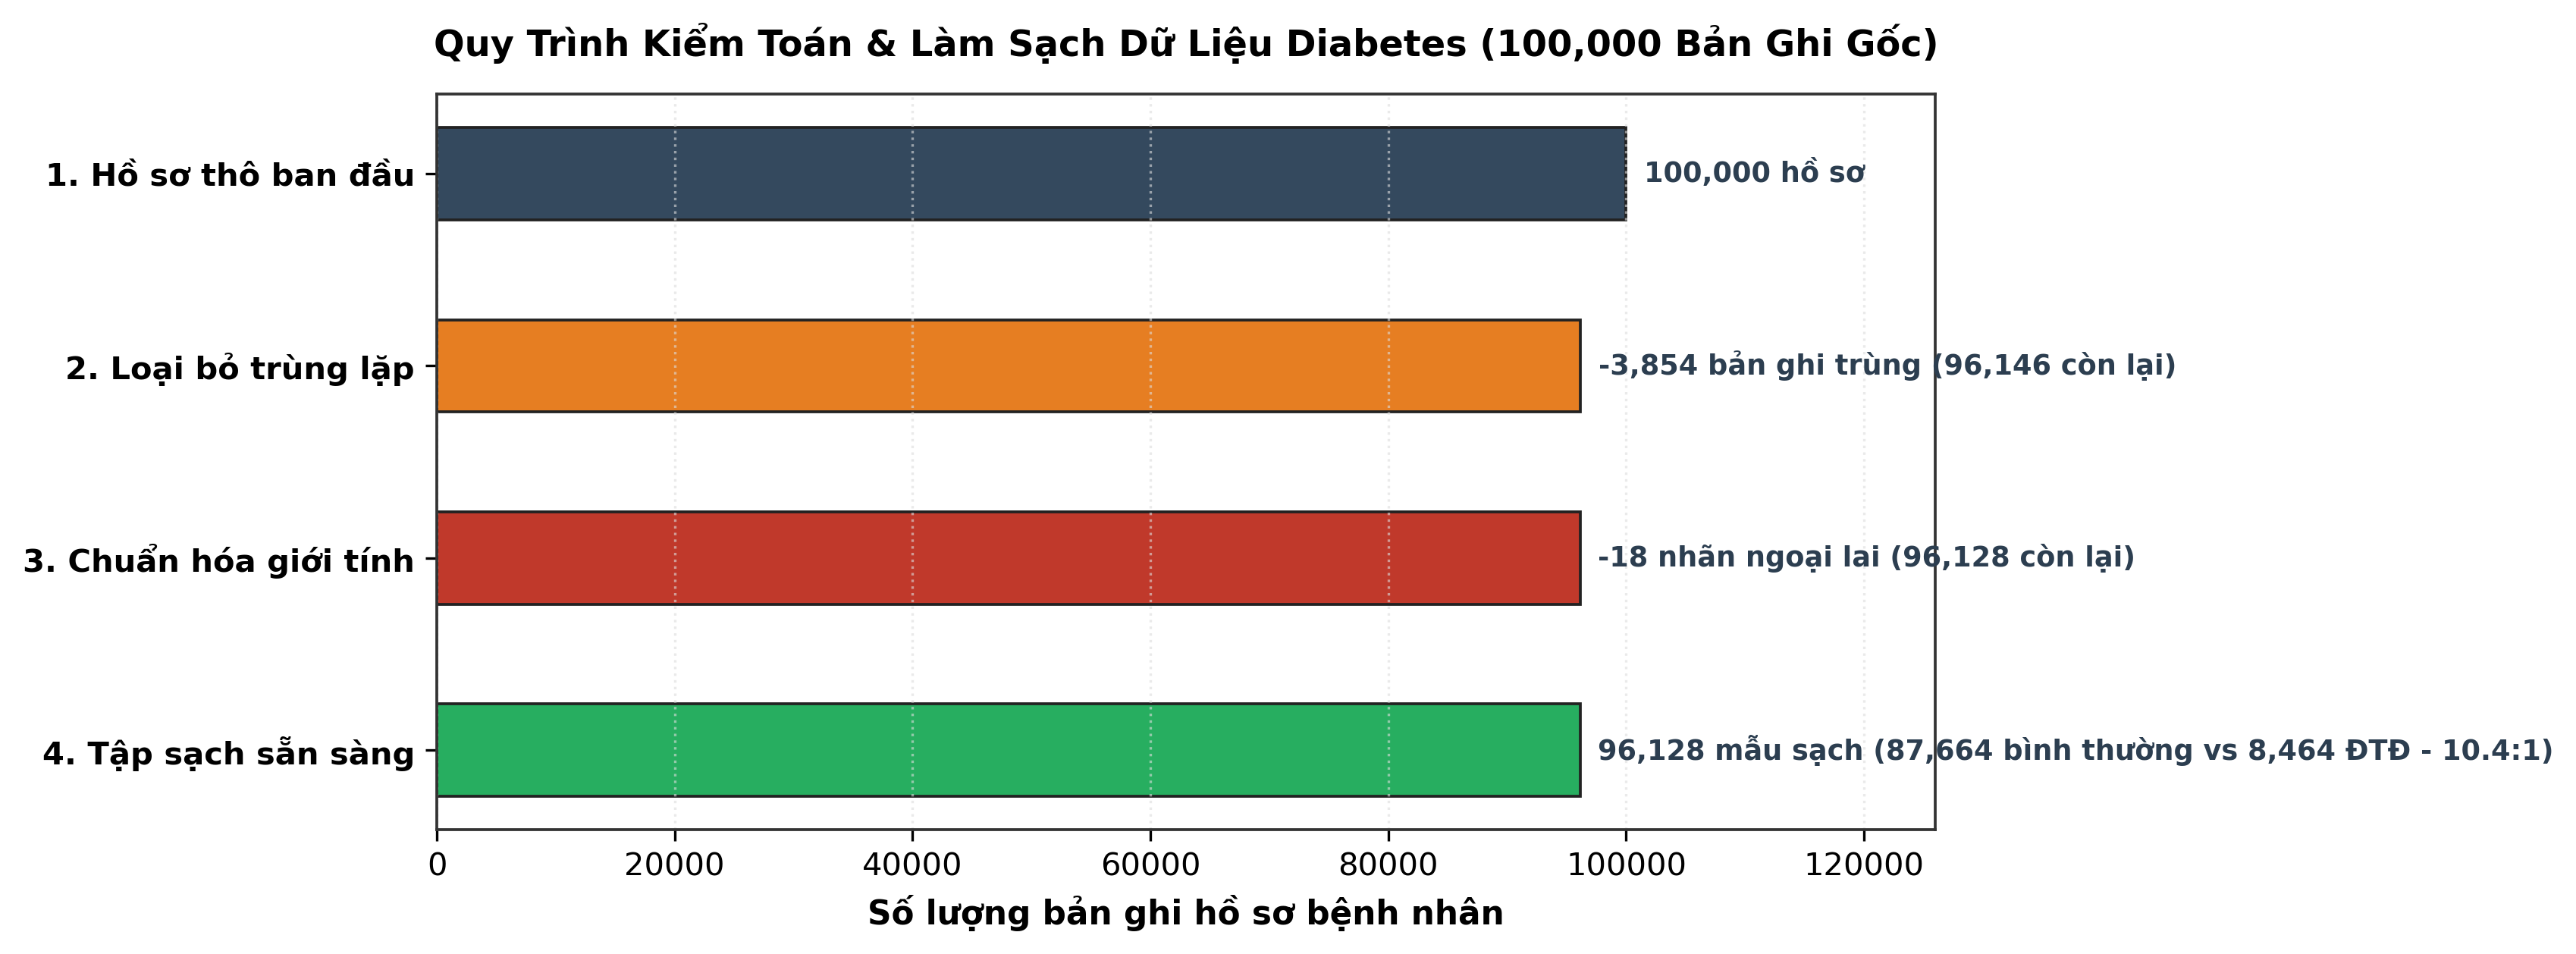
\includegraphics[width=0.88\textwidth]{images/fig401_diabetes_cleaning_funnel.png}
    \caption{Quy trình kiểm toán, khử trùng lặp và làm sạch tập dữ liệu Diabetes từ 100,000 bản ghi gốc xuống 96,128 mẫu sạch chuẩn hóa, phản ánh tỷ lệ mất cân bằng dịch tễ tự nhiên 10.4 : 1.}
    \label{fig:diabetes_cleaning_funnel}
\end{figure}

\subsection{Phân Tích Chỉ Số Sinh Hóa \& Tương Quan Bệnh Lý}
Hai biến số sinh hóa then chốt mang tính quyết định trong chẩn đoán lâm sàng là \texttt{HbA1c\_level} (chỉ số đường huyết tích lũy 3 tháng) và \texttt{blood\_glucose\_level} (nồng độ đường huyết tức thời):
\begin{itemize}[leftmargin=*]
    \item \textbf{Chỉ số HbA1c:} Phân bố mật độ xác suất KDE (Hình \ref{fig:diabetes_biomarker_kde}) thể hiện sự phân tách rõ rệt giữa hai nhóm dân số. Nhóm người bình thường có trung vị $\text{HbA1c} = 5.8\%$ (nằm dưới ngưỡng cảnh báo y khoa $5.7\% - 6.4\%$). Ngược lại, nhóm người mắc đái tháo đường có trung vị vọt lên $\text{HbA1c} = 6.6\%$ và trung bình $6.93\%$, vượt qua ngưỡng chẩn đoán đái tháo đường lâm sàng theo tiêu chuẩn ADA ($\ge 6.5\%$).
    \item \textbf{Đường huyết tức thời (Blood Glucose):} Nhóm không mắc bệnh có nồng độ trung bình $132.8\,\text{mg/dL}$ (trung vị $140.0\,\text{mg/dL}$), trong khi nhóm mắc bệnh đạt mức trung bình $194.0\,\text{mg/dL}$ (trung vị $160.0\,\text{mg/dL}$), vượt xa ngưỡng đường huyết lúc đói chuẩn ($126.0\,\text{mg/dL}$).
    \item \textbf{Phân tích tương quan Pearson (Hình \ref{fig:diabetes_correlation_matrix}):} Hai chỉ số \texttt{blood\_glucose\_level} ($r=0.42$) và \texttt{HbA1c\_level} ($r=0.41$) có hệ số tương quan tuyến tính mạnh nhất với biến mục tiêu \texttt{diabetes}. Tiếp theo là các yếu tố nhân khẩu học và bệnh lý nền gồm \texttt{age} ($r=0.26$), \texttt{bmi} ($r=0.21$), \texttt{hypertension} ($r=0.20$) và \texttt{heart\_disease} ($r=0.17$).
\end{itemize}

\begin{table}[H]
\centering
\caption{Thống kê mô tả định lượng 8 biến đặc trưng của tập dữ liệu Diabetes (96,128 mẫu sạch).}
\label{tab:diabetes_stats}
\small
\setlength{\tabcolsep}{6pt}
\begin{tabularx}{\textwidth}{lcccccX}
\toprule
\textbf{Thuộc tính} & \textbf{Min} & \textbf{Max} & \textbf{Mean} & \textbf{Median} & \textbf{Std} & \textbf{Tương quan ($r$)} \\
\midrule
Gender (Giới tính)          & $0.0$  & $1.0$   & $0.42$   & $0.0$   & $0.49$  & $+0.04$ (Nữ 60.9\%, Nam 39.1\%) \\
Age (Tuổi)                 & $0.08$ & $80.0$  & $41.80$  & $43.0$  & $22.46$ & $+0.26$ (Người bệnh trung vị 62 tuổi) \\
Hypertension (Tăng HA)     & $0.0$  & $1.0$   & $0.08$   & $0.0$   & $0.27$  & $+0.20$ (Tỷ lệ mắc 7.5\%) \\
Heart Disease (Tim mạch)   & $0.0$  & $1.0$   & $0.04$   & $0.0$   & $0.20$  & $+0.17$ (Tỷ lệ mắc 3.9\%) \\
Smoking History (Hút thuốc)& $0.0$  & $2.0$   & $0.44$   & $0.0$   & $0.72$  & $+0.07$ (Thang nguy cơ 0, 1, 2) \\
BMI (Chỉ số thể trọng)     & $10.01$& $95.69$ & $27.32$  & $27.32$ & $6.77$  & $+0.21$ (Người bệnh trung bình 32.0) \\
HbA1c Level (\%)           & $3.50$ & $9.00$  & $5.53$   & $5.80$  & $1.07$  & $+0.41$ (Ngưỡng chẩn đoán $\ge 6.5\%$) \\
Blood Glucose (mg/dL)      & $80.0$ & $300.0$ & $138.22$ & $140.0$ & $40.91$ & $+0.42$ (Dấu hiệu sinh hóa chủ đạo) \\
\midrule
\multicolumn{7}{l}{\textbf{Biến mục tiêu Diabetes: } $96,128$ mẫu sạch ($87,664$ âm tính -- $91.2\%$; $8,464$ dương tính -- $8.8\%$)} \\
\bottomrule
\end{tabularx}
\end{table}

\begin{figure}[H]
    \centering
    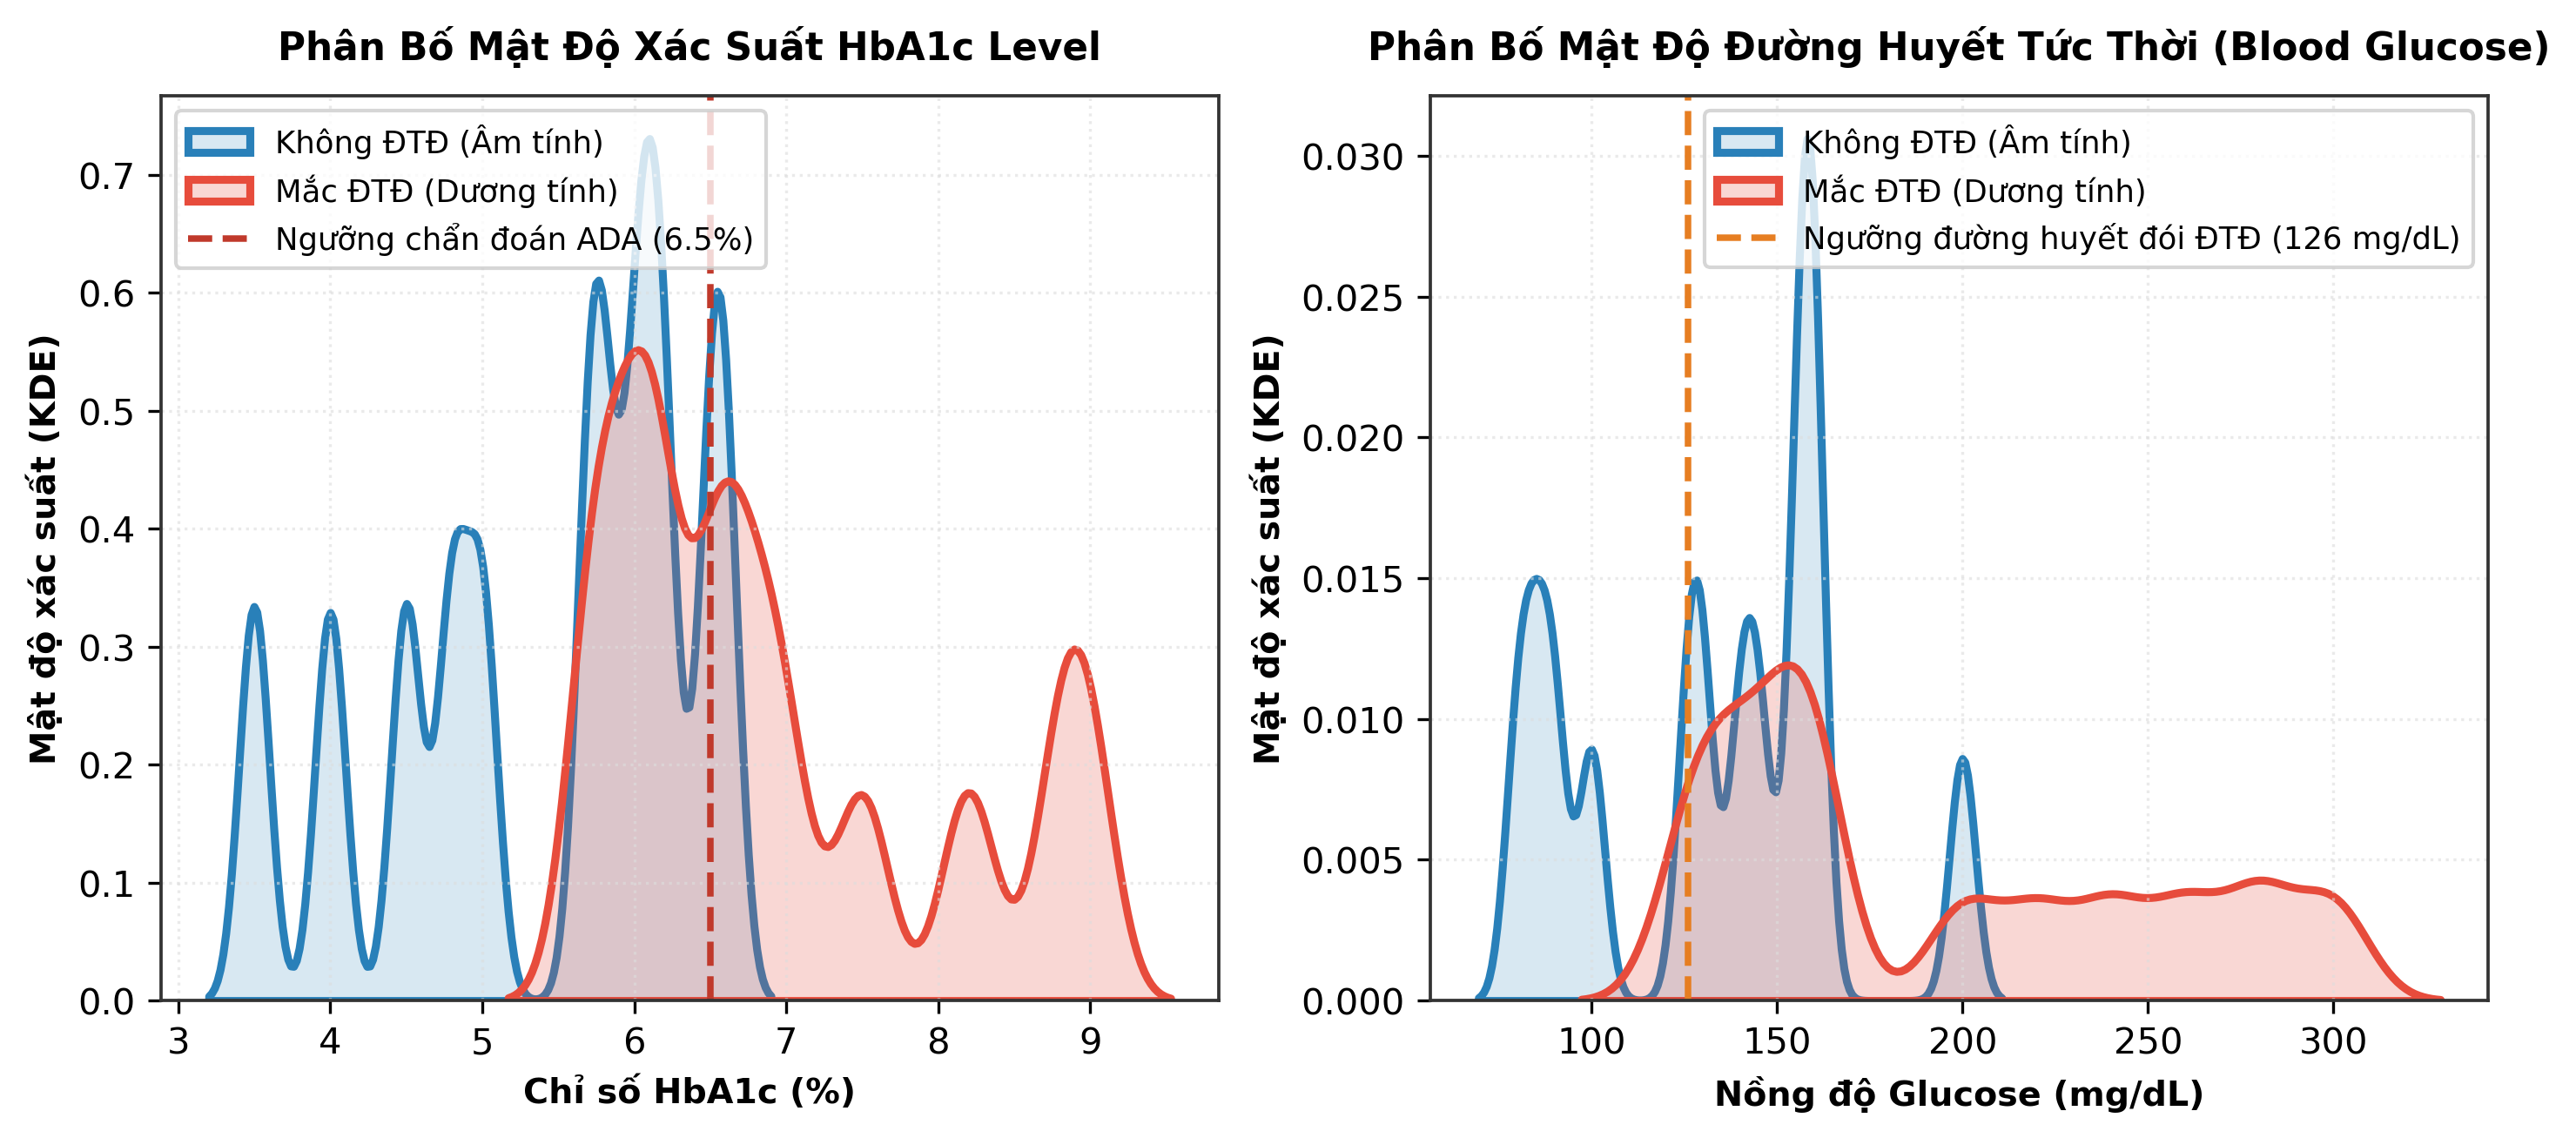
\includegraphics[width=0.92\textwidth]{images/fig402_diabetes_biomarker_kde.png}
    \caption{Phân tích phân bố mật độ xác suất (KDE) của hai chỉ số sinh hóa chủ đạo: HbA1c (\%) và Blood Glucose (mg/dL) phân tầng theo nhãn lâm sàng Không ĐTĐ (xanh) và Mắc ĐTĐ (đỏ), làm rõ tính phân tách mạnh mẽ tại các ngưỡng y khoa.}
    \label{fig:diabetes_biomarker_kde}
\end{figure}

\begin{figure}[H]
    \centering
    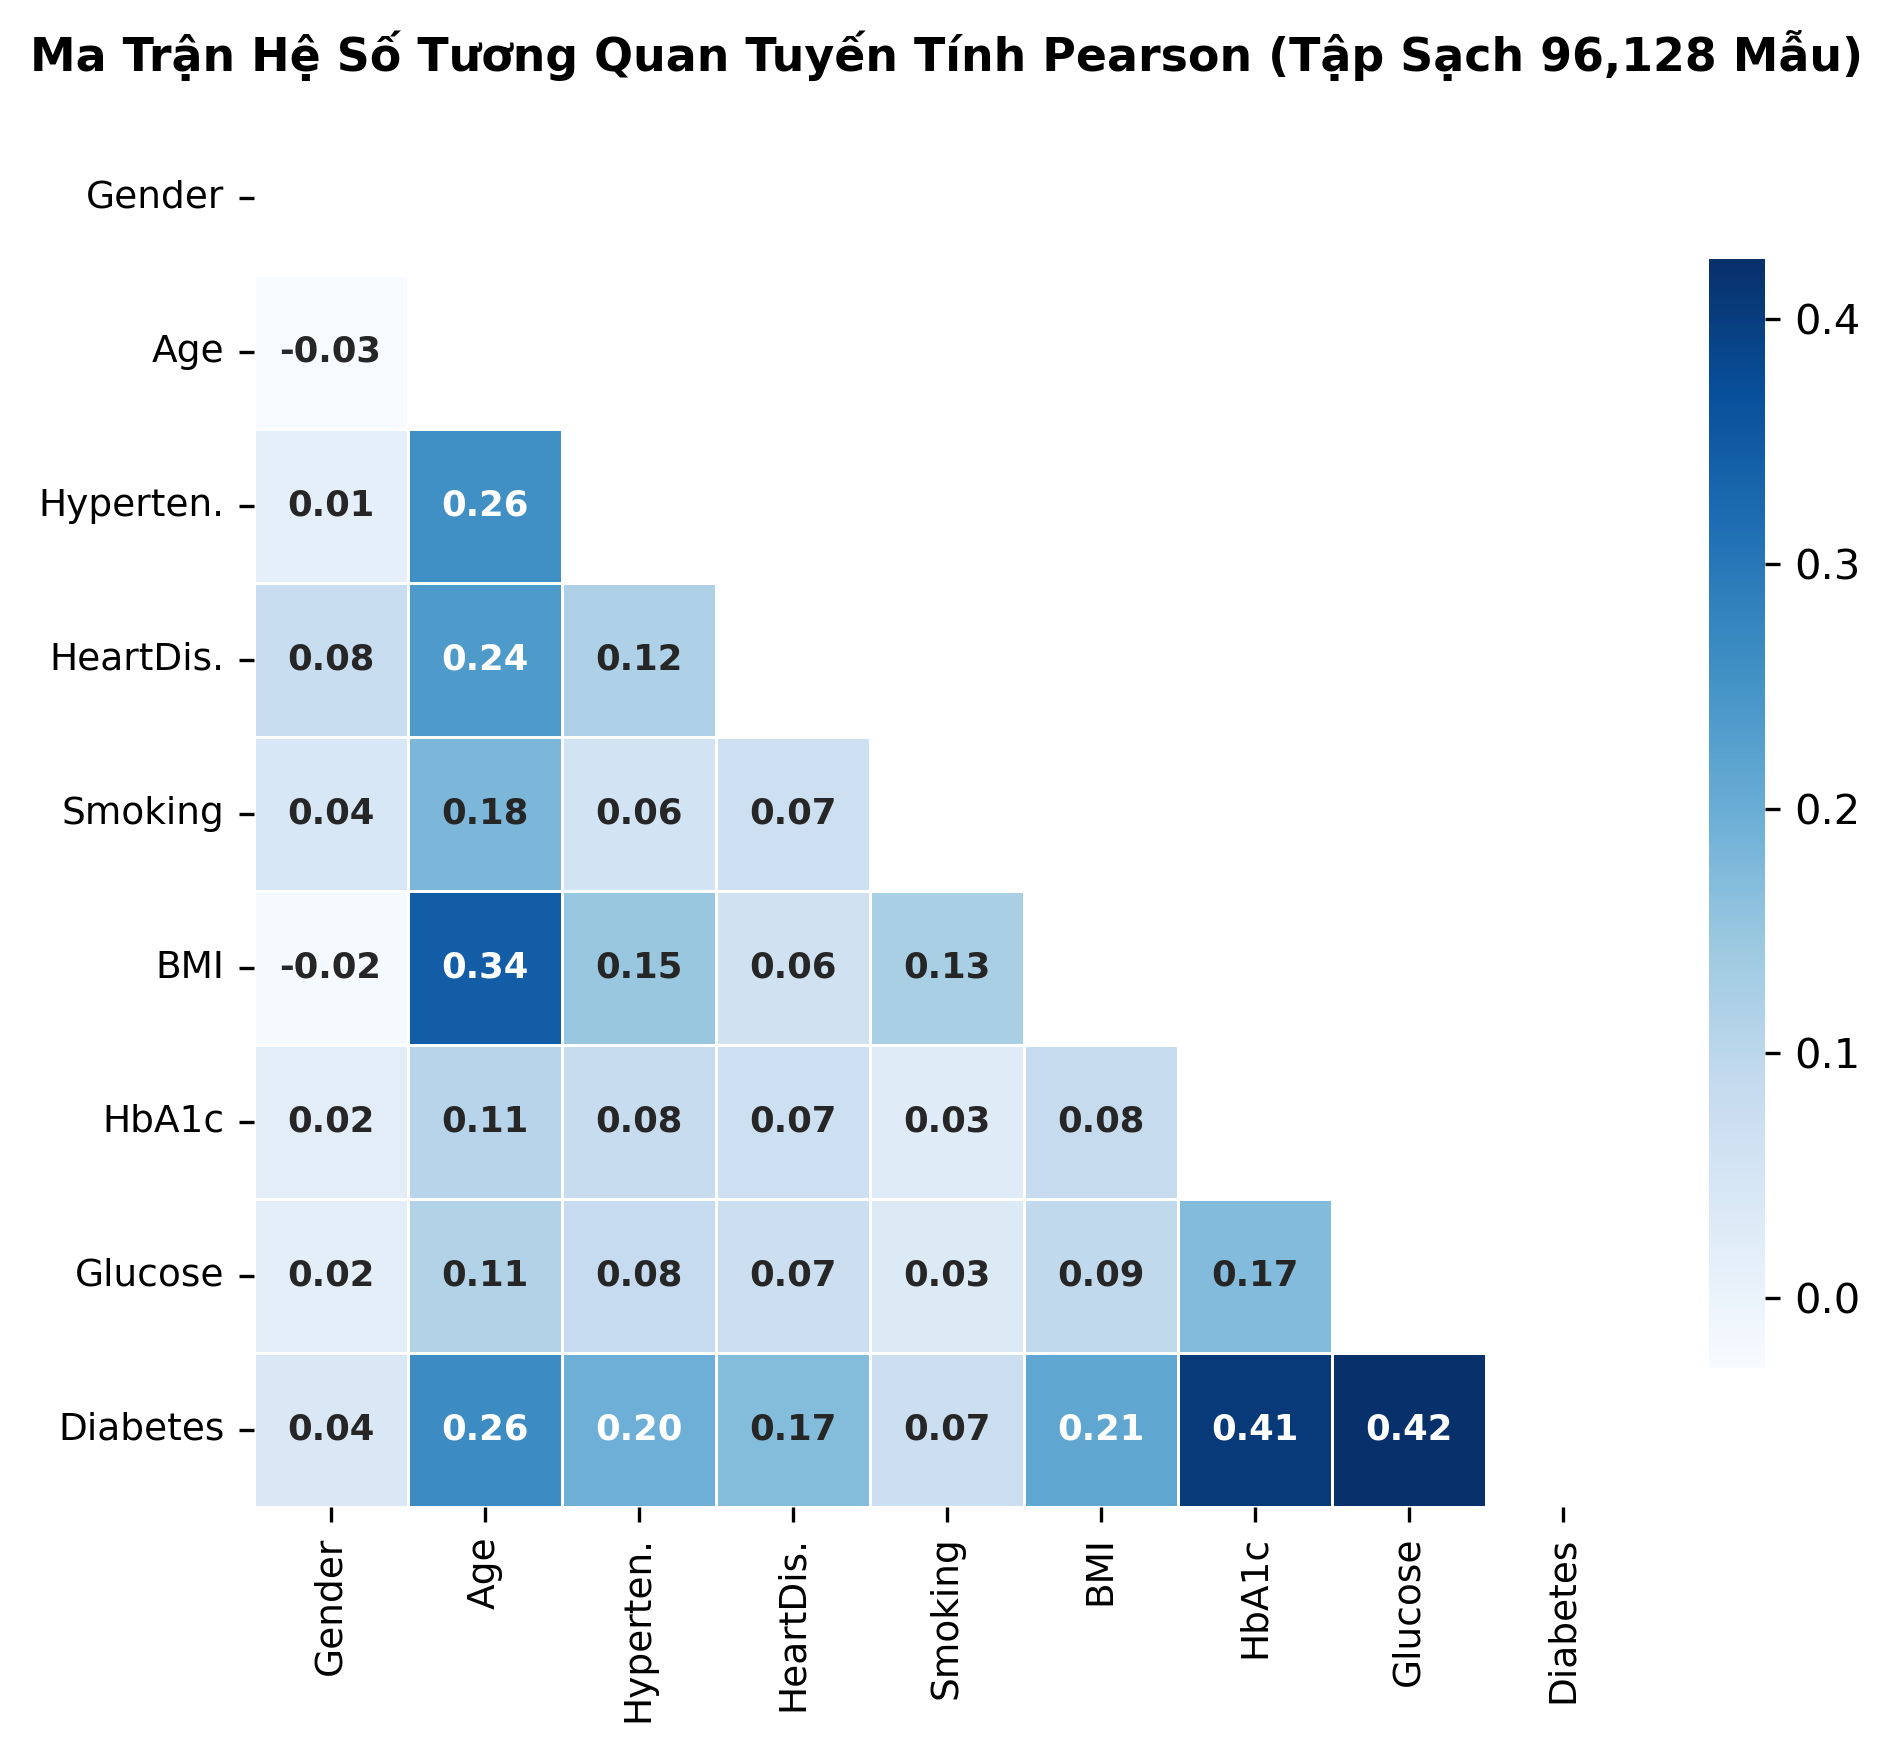
\includegraphics[width=0.68\textwidth]{images/fig403_diabetes_correlation_matrix.png}
    \caption{Ma trận hệ số tương quan tuyến tính Pearson giữa 8 thuộc tính lâm sàng và biến mục tiêu Diabetes trên tập 96,128 mẫu sạch.}
    \label{fig:diabetes_correlation_matrix}
\end{figure}

\subsection{Thiết Lập Pipeline Chuẩn Hóa \& Định Dạng Tensor Cho Mạng Nơ-ron Tích Chập 1 Chiều (1D-CNN)}
Khác với các mô hình cây quyết định truyền thống, để áp dụng mạng tích chập cho dữ liệu bảng y sinh, chuỗi 8 thuộc tính lâm sàng sau khi chuẩn hóa bằng \texttt{StandardScaler} được cấu trúc thành tensor 3 chiều chuyên biệt cho mạng tích chập 1 chiều (\textbf{1D-CNN}):
\begin{equation}
    \mathbf{X} \in \mathbb{R}^{N \times C_{\text{in}} \times L} = \mathbb{R}^{N \times 1 \times 8}
\end{equation}
trong đó $N$ là kích thước batch, $C_{\text{in}} = 1$ đóng vai trò là số kênh tín hiệu đầu vào, và $L = 8$ là chiều dài của chuỗi đặc trưng y sinh.

\textbf{Cơ chế trích xuất đặc trưng của 1D-CNN trên dữ liệu y sinh:} Bộ lọc tích chập 1 chiều $\mathbf{W} \in \mathbb{R}^{C_{\text{out}} \times C_{\text{in}} \times K}$ (với kích thước kernel $K \in \{2, 3\}$) sẽ trượt tuần tự dọc theo chuỗi 8 đặc trưng. Phép tính tích chập 1D tại vị trí $i$ được định nghĩa:
\begin{equation}
    (\mathbf{X} * \mathbf{W})[i] = \sum_{k=0}^{K-1} \mathbf{X}[i + k] \cdot \mathbf{W}[k] + b
\end{equation}
Cơ chế này cho phép mạng nơ-ron học được các mối liên kết phi tuyến cục bộ giữa các cặp thuộc tính sinh hóa lân cận (ví dụ: mối liên hệ cộng hưởng giữa nồng độ Glucose và chỉ số HbA1c, hay tương tác giữa huyết áp, BMI và tuổi tác) trước khi tổng hợp qua các tầng gộp toàn cục (Global Average Pooling 1D).

Đoạn mã \ref{lst:diabetes_pipeline} hiện thực hóa toàn bộ pipeline làm sạch, phân chia phân tầng $80:20$, chuẩn hóa Z-score và đóng gói tensor cho mạng 1D-CNN.

\begin{lstlisting}[language=Python, caption={Pipeline nạp dữ liệu, làm sạch, chuẩn hóa và đóng gói DataLoader cho 1D-CNN trên tập Diabetes 100k mẫu.}, label={lst:diabetes_pipeline}]
import torch
import numpy as np
import pandas as pd
from torch.utils.data import TensorDataset, DataLoader
from sklearn.model_selection import train_test_split
from sklearn.preprocessing import StandardScaler

def prepare_diabetes_dataloaders(csv_path="data/diabetes_prediction_dataset.csv", 
                                 batch_size=64, test_size=0.2, random_state=42):
    # 1. Nap tap du lieu bang va khu trung lap
    df = pd.read_csv(csv_path)
    df = df.drop_duplicates()
    df = df[df['gender'] != 'Other'].copy()
    
    # 2. Ma hoa dac trung phan loai
    df['gender'] = (df['gender'] == 'Male').astype(np.float32)
    smoking_map = {'never': 0.0, 'No Info': 0.0, 'former': 1.0, 
                   'not current': 1.0, 'current': 2.0, 'ever': 2.0}
    df['smoking_history'] = df['smoking_history'].map(smoking_map).fillna(0.0).astype(np.float32)
    
    features = ['gender', 'age', 'hypertension', 'heart_disease', 
                'smoking_history', 'bmi', 'HbA1c_level', 'blood_glucose_level']
    X = df[features].values.astype(np.float32)
    y = df['diabetes'].values.astype(np.int64)
    
    # 3. Phan chia tap Huan luyen / Kiem tra co phan tang (Stratified Split 80:20)
    X_train, X_test, y_train, y_test = train_test_split(
        X, y, test_size=test_size, stratify=y, random_state=random_state
    )
    
    # 4. Chuan hoa dac trung bang StandardScaler
    scaler = StandardScaler()
    X_train = scaler.fit_transform(X_train)
    X_test = scaler.transform(X_test)
    
    # 5. Dinh dang tensor chuyen biet cho mang tich chap 1 chieu (1D-CNN): (N, 1, 8)
    X_train = X_train[:, np.newaxis, :]  # Shape: (Batch, Channels=1, Length=8)
    X_test = X_test[:, np.newaxis, :]
    
    # 6. Dong goi PyTorch TensorDataset & DataLoader
    train_dataset = TensorDataset(torch.from_numpy(X_train), torch.from_numpy(y_train))
    test_dataset = TensorDataset(torch.from_numpy(X_test), torch.from_numpy(y_test))
    
    train_loader = DataLoader(train_dataset, batch_size=batch_size, shuffle=True, pin_memory=True)
    test_loader = DataLoader(test_dataset, batch_size=batch_size, shuffle=False, pin_memory=True)
    
    return train_loader, test_loader, scaler
\end{lstlisting}

% =========================================================================
% 4.3. SVHN
% =========================================================================
\section{Khảo Sát, Phân Tích \& Chuẩn Hóa Bộ Dữ Liệu Ảnh Ngoại Cảnh SVHN}

\subsection{Đặc Tính Hình Thái Học \& Thách Thức Thị Giác Tự Nhiên}
Tập dữ liệu Street View House Numbers (SVHN) là bộ dữ liệu thị giác thực tế được xây dựng bởi Đại học Stanford, bao gồm các ảnh chụp số nhà thực tế từ hệ thống xe chụp phố Google Street View. Mỗi mẫu ảnh là một ma trận 3 chiều kích thước $32 \times 32 \times 3$ biểu diễn hệ màu RGB. Khác với tập chữ số viết tay MNIST đã được quy chuẩn hóa về định dạng ảnh xám đơn sắc với chữ số nằm cô lập trên nền đen, SVHN mang các đặc tính phong phú và phức tạp của ảnh chụp ngoại cảnh thực tế (Hình \ref{fig:svhn_sample_grid}):
\begin{itemize}[leftmargin=*]
    \item \textbf{Nhiễu nền đa dạng và phức tạp:} Nền ảnh là bề mặt tường gạch, cửa gỗ, thanh chắn kim loại, kính phản quang, hoặc bóng cây đổ lộn xộn.
    \item \textbf{Chênh lệch độ tương phản cực lớn:} Một số ảnh chụp trực diện dưới ánh nắng gay gắt dẫn đến hiện tượng chói sáng (overexposure); ngược lại, nhiều ảnh chụp trong bóng râm hoặc lúc hoàng hôn có độ sáng cực thấp.
    \item \textbf{Chữ số nhiễu lân cận (Distracting Neighboring Digits):} Do được cắt tự động từ các biển số nhà có nhiều chữ số (ví dụ số nhà ``23'', ``194''), chữ số mục tiêu nằm ở trung tâm nhưng hai bên lề thường xuất hiện một phần của các chữ số kế cận. Mạng CNN buộc phải học được cơ chế tập trung không gian vào trung tâm thay vì bị đánh lừa bởi rìa ảnh.
    \item \textbf{Biến dạng phối cảnh và góc nghiêng:} Biển số nhà thường được chụp từ góc xiên của xe cơ giới, tạo ra độ nghiêng không gian 3D và biến dạng quang học dạng hình thang.
\end{itemize}

\begin{figure}[H]
    \centering
    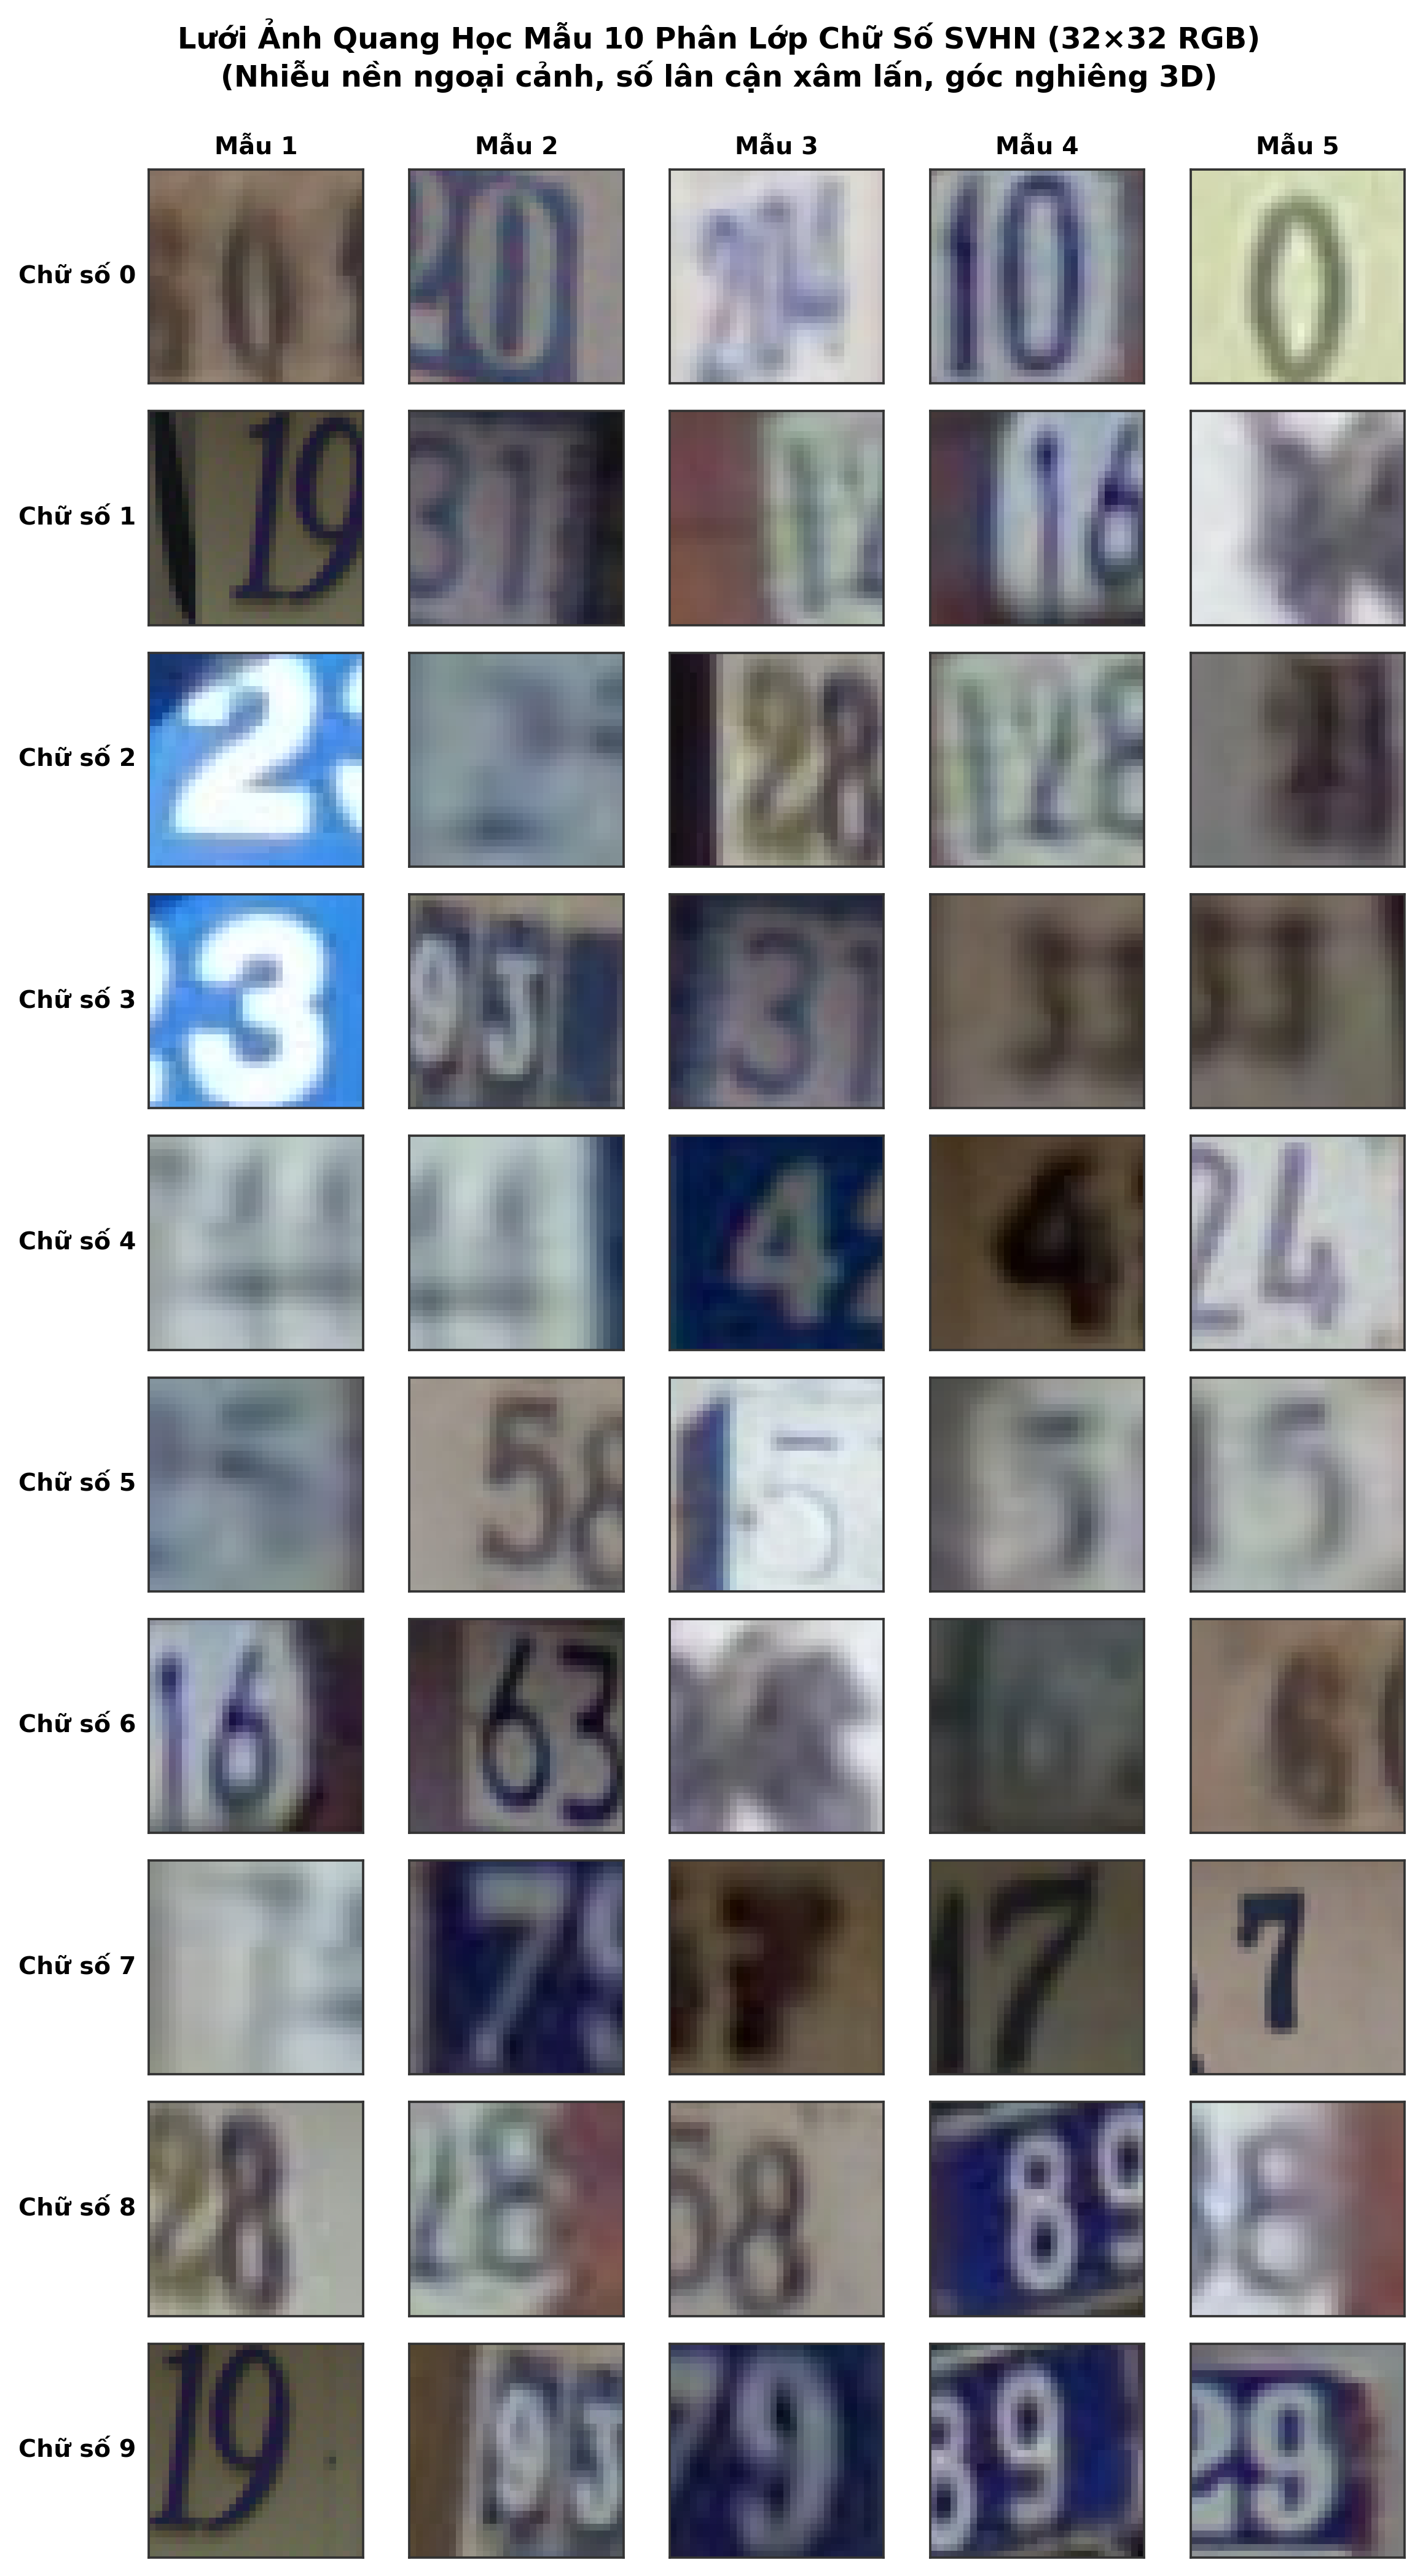
\includegraphics[width=0.78\textwidth]{images/fig404_svhn_sample_grid.png}
    \caption{Lưới ảnh quang học mẫu 10 phân lớp chữ số ngoại cảnh thực tế SVHN ($32 \times 32 \times 3$ RGB) minh họa nhiễu nền đô thị, chữ số lân cận xâm lấn và biến thiên góc chụp 3D.}
    \label{fig:svhn_sample_grid}
\end{figure}

\subsection{Phân Bố Tần Suất Lớp Chữ Số \& Hiện Tượng Lệch Tự Nhiên}
Khảo sát phân bố số lượng mẫu trên tập huấn luyện ($73,257$ ảnh) và tập kiểm tra ($26,032$ ảnh) cho thấy hiện tượng mất cân bằng lớp tự nhiên (Natural Class Imbalance) phản ánh đúng quy luật thống kê của số nhà dân dụng (Bảng \ref{tab:svhn_stats} và Hình \ref{fig:svhn_class_distribution}). Chữ số $1$ chiếm tỷ lệ áp đảo nhất ($18.92\%$ tập train với $13,861$ ảnh), tiếp theo là chữ số $2$ ($14.45\%$), trong khi chữ số $9$ chỉ chiếm $6.36\%$ ($4,659$ ảnh) và số $0$ chiếm $6.75\%$ ($4,948$ ảnh).

\begin{table}[H]
\centering
\caption{Phân bố số lượng và tỷ lệ mẫu 10 lớp chữ số của tập dữ liệu SVHN.}
\label{tab:svhn_stats}
\small
\setlength{\tabcolsep}{5pt}
\begin{tabularx}{\textwidth}{lccccX}
\toprule
\textbf{Nhãn} & \textbf{Train ($N$)} & \textbf{\% Train} & \textbf{Test ($N$)} & \textbf{\% Test} & \textbf{Đặc trưng nhận diện quang học} \\
\midrule
Chữ số 0 & $4,948$  & $6.75\%$  & $1,744$ & $6.70\%$  & Cấu trúc vòng khép kín elip, dễ nhầm với số 8, 6 \\
Chữ số 1 & $13,861$ & $18.92\%$ & $5,099$ & $19.59\%$ & Nét thẳng đứng mảnh, tần suất xuất hiện cao nhất \\
Chữ số 2 & $10,585$ & $14.45\%$ & $4,149$ & $15.94\%$ & Nét cong vòm trên nối với đường chân ngang đáy \\
Chữ số 3 & $8,497$  & $11.60\%$ & $2,882$ & $11.07\%$ & Hai vòng cung mở sang trái, thắt eo giữa \\
Chữ số 4 & $7,458$  & $10.18\%$ & $2,523$ & $9.69\%$  & Giao điểm tam giác vuông hoặc chữ thập hở \\
Chữ số 5 & $6,882$  & $9.39\%$  & $2,384$ & $9.16\%$  & Nét ngang đỉnh kết hợp bụng cong dưới \\
Chữ số 6 & $5,727$  & $7.82\%$  & $1,977$ & $7.59\%$  & Vòng tròn đáy nối đuôi cong lên, nhầm với số 0 \\
Chữ số 7 & $5,595$  & $7.64\%$  & $2,019$ & $7.76\%$  & Nét ngang trên và nét chéo dốc xuống \\
Chữ số 8 & $5,045$  & $6.89\%$  & $1,660$ & $6.38\%$  & Cấu trúc hai vòng tròn thắt eo đối xứng \\
Chữ số 9 & $4,659$  & $6.36\%$  & $1,595$ & $6.13\%$  & Vòng tròn đỉnh nối đuôi thẳng buông xuống \\
\bottomrule
\end{tabularx}
\end{table}

\begin{figure}[H]
    \centering
    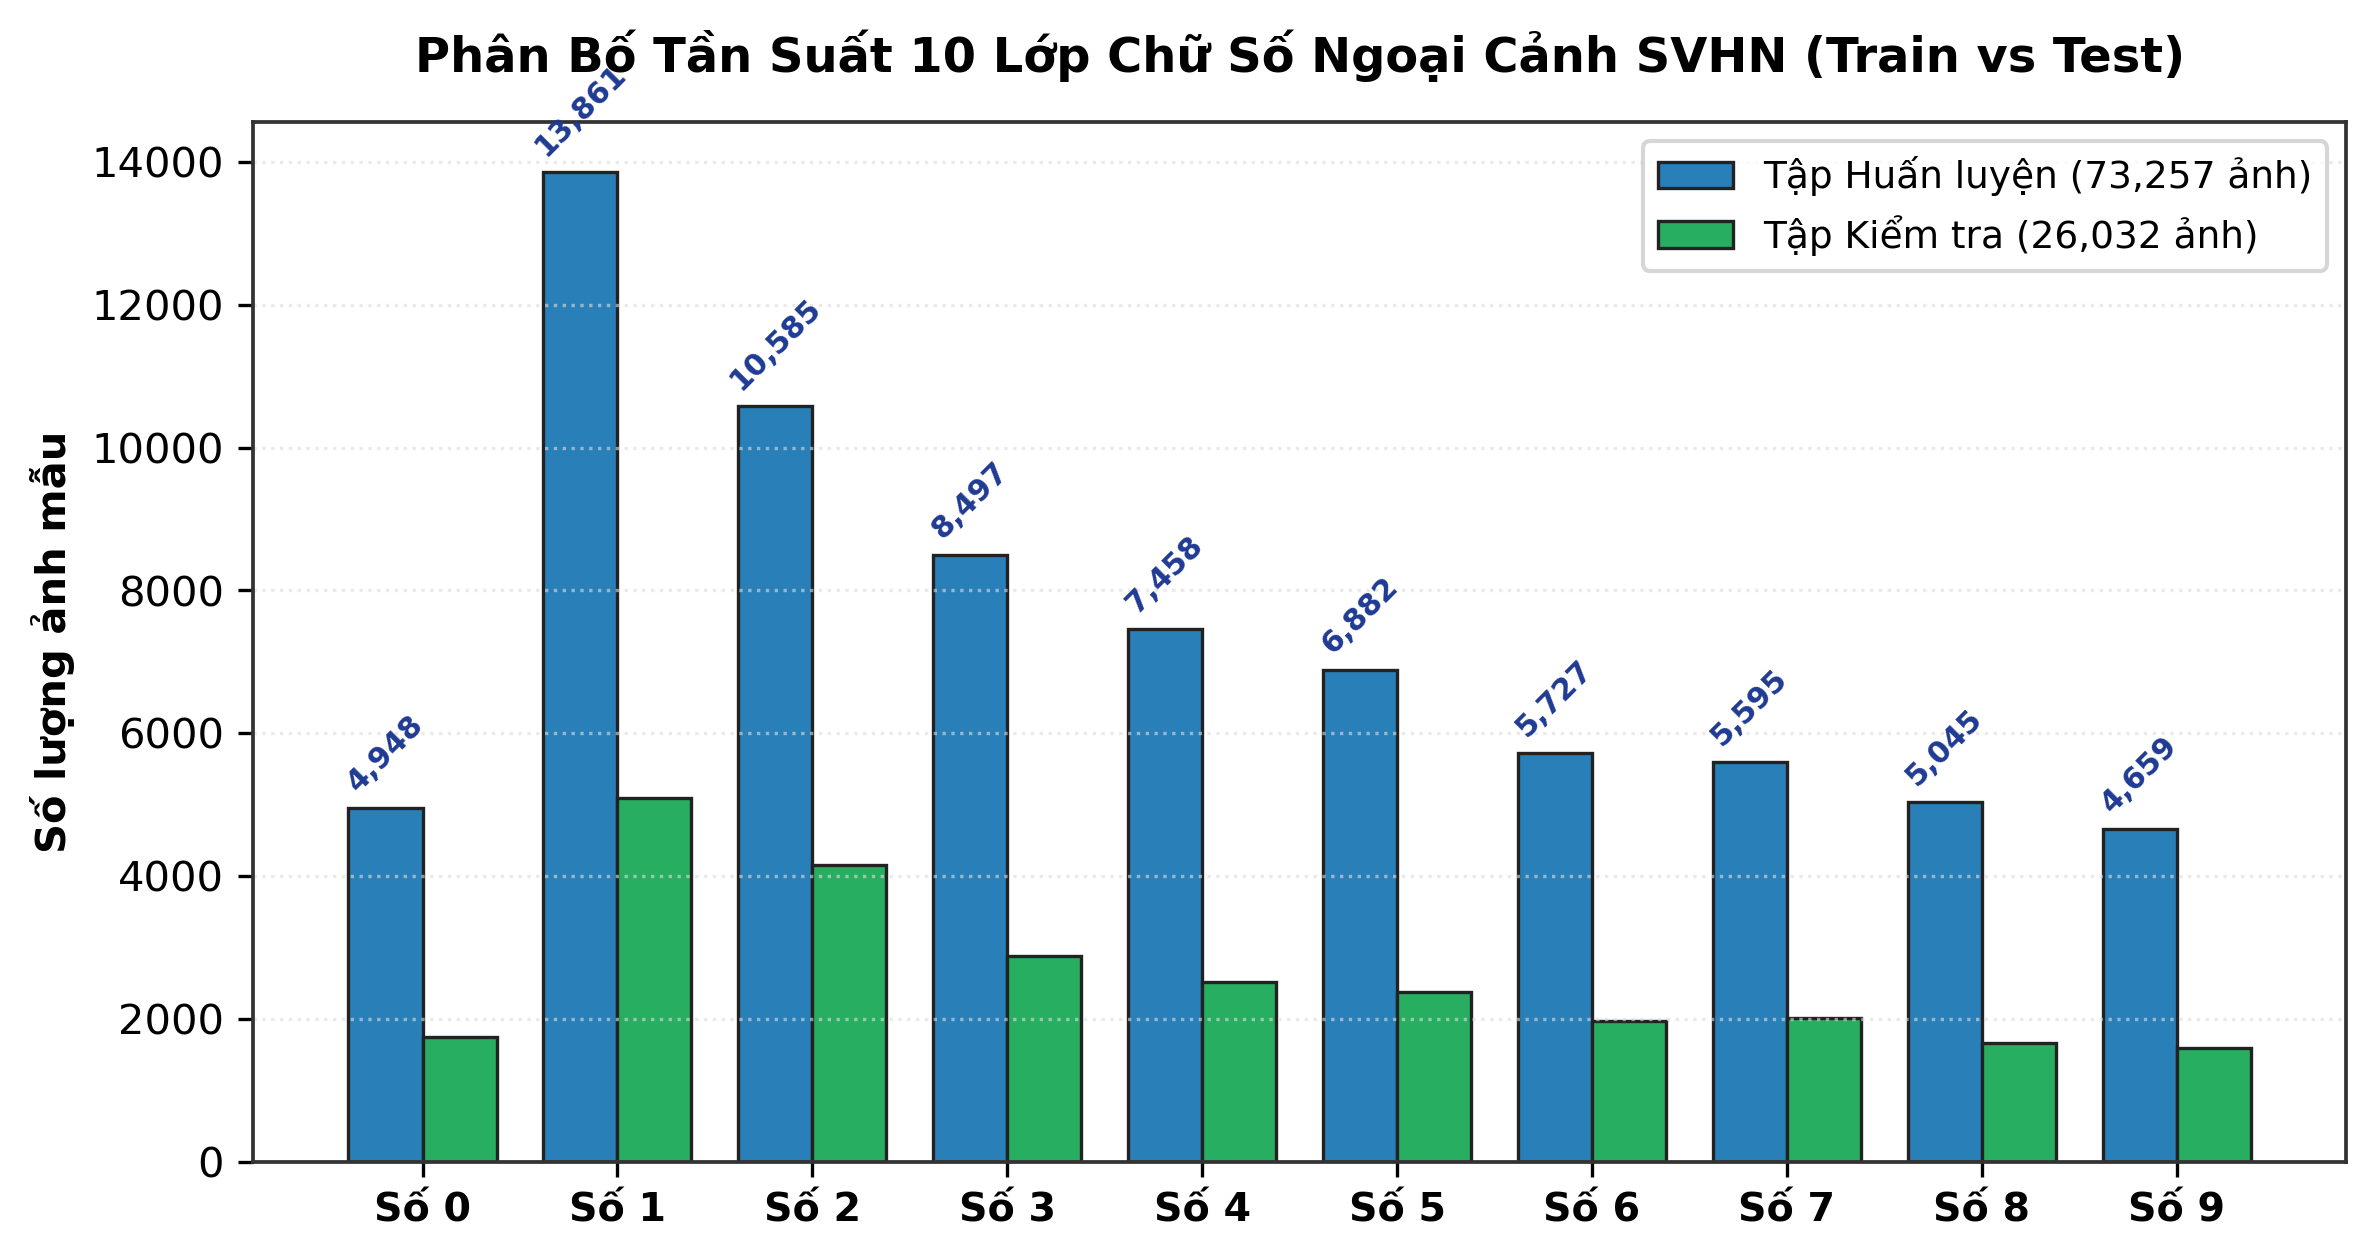
\includegraphics[width=0.85\textwidth]{images/fig405_svhn_class_distribution.png}
    \caption{Biểu đồ phân bố tần suất 10 lớp chữ số ngoại cảnh SVHN giữa tập huấn luyện (73,257 ảnh) và tập kiểm tra (26,032 ảnh).}
    \label{fig:svhn_class_distribution}
\end{figure}

\subsection{Trích Xuất Tham Số Chuẩn Hóa Kênh Màu \& Chiến Lược Tăng Cường Ảnh}
Từ việc tính toán mật độ trên toàn bộ không gian ảnh chuẩn hóa $[0, 1]$ (Hình \ref{fig:svhn_rgb_channel_histograms}), chúng tôi thu được bộ tham số trung bình ($\mu$) và độ lệch chuẩn ($\sigma$) của 3 kênh màu:
\begin{equation}
    \boldsymbol{\mu}_{\text{SVHN}} = [0.435, \, 0.440, \, 0.469], \quad \boldsymbol{\sigma}_{\text{SVHN}} = [0.192, \, 0.193, \, 0.190]
\end{equation}
Đặc biệt, kênh Blue ($\mu=0.469$) có độ sáng trung bình cao hơn hai kênh còn lại do ảnh hưởng của phản xạ nền trời xanh và màu sơn biển số xe/nhà phổ biến. Việc chuẩn hóa theo đúng giá trị $\boldsymbol{\mu}_{\text{SVHN}}$ và $\boldsymbol{\sigma}_{\text{SVHN}}$ là điều kiện tiên quyết để đảm bảo gradient truyền ngược đồng đều.

\begin{figure}[H]
    \centering
    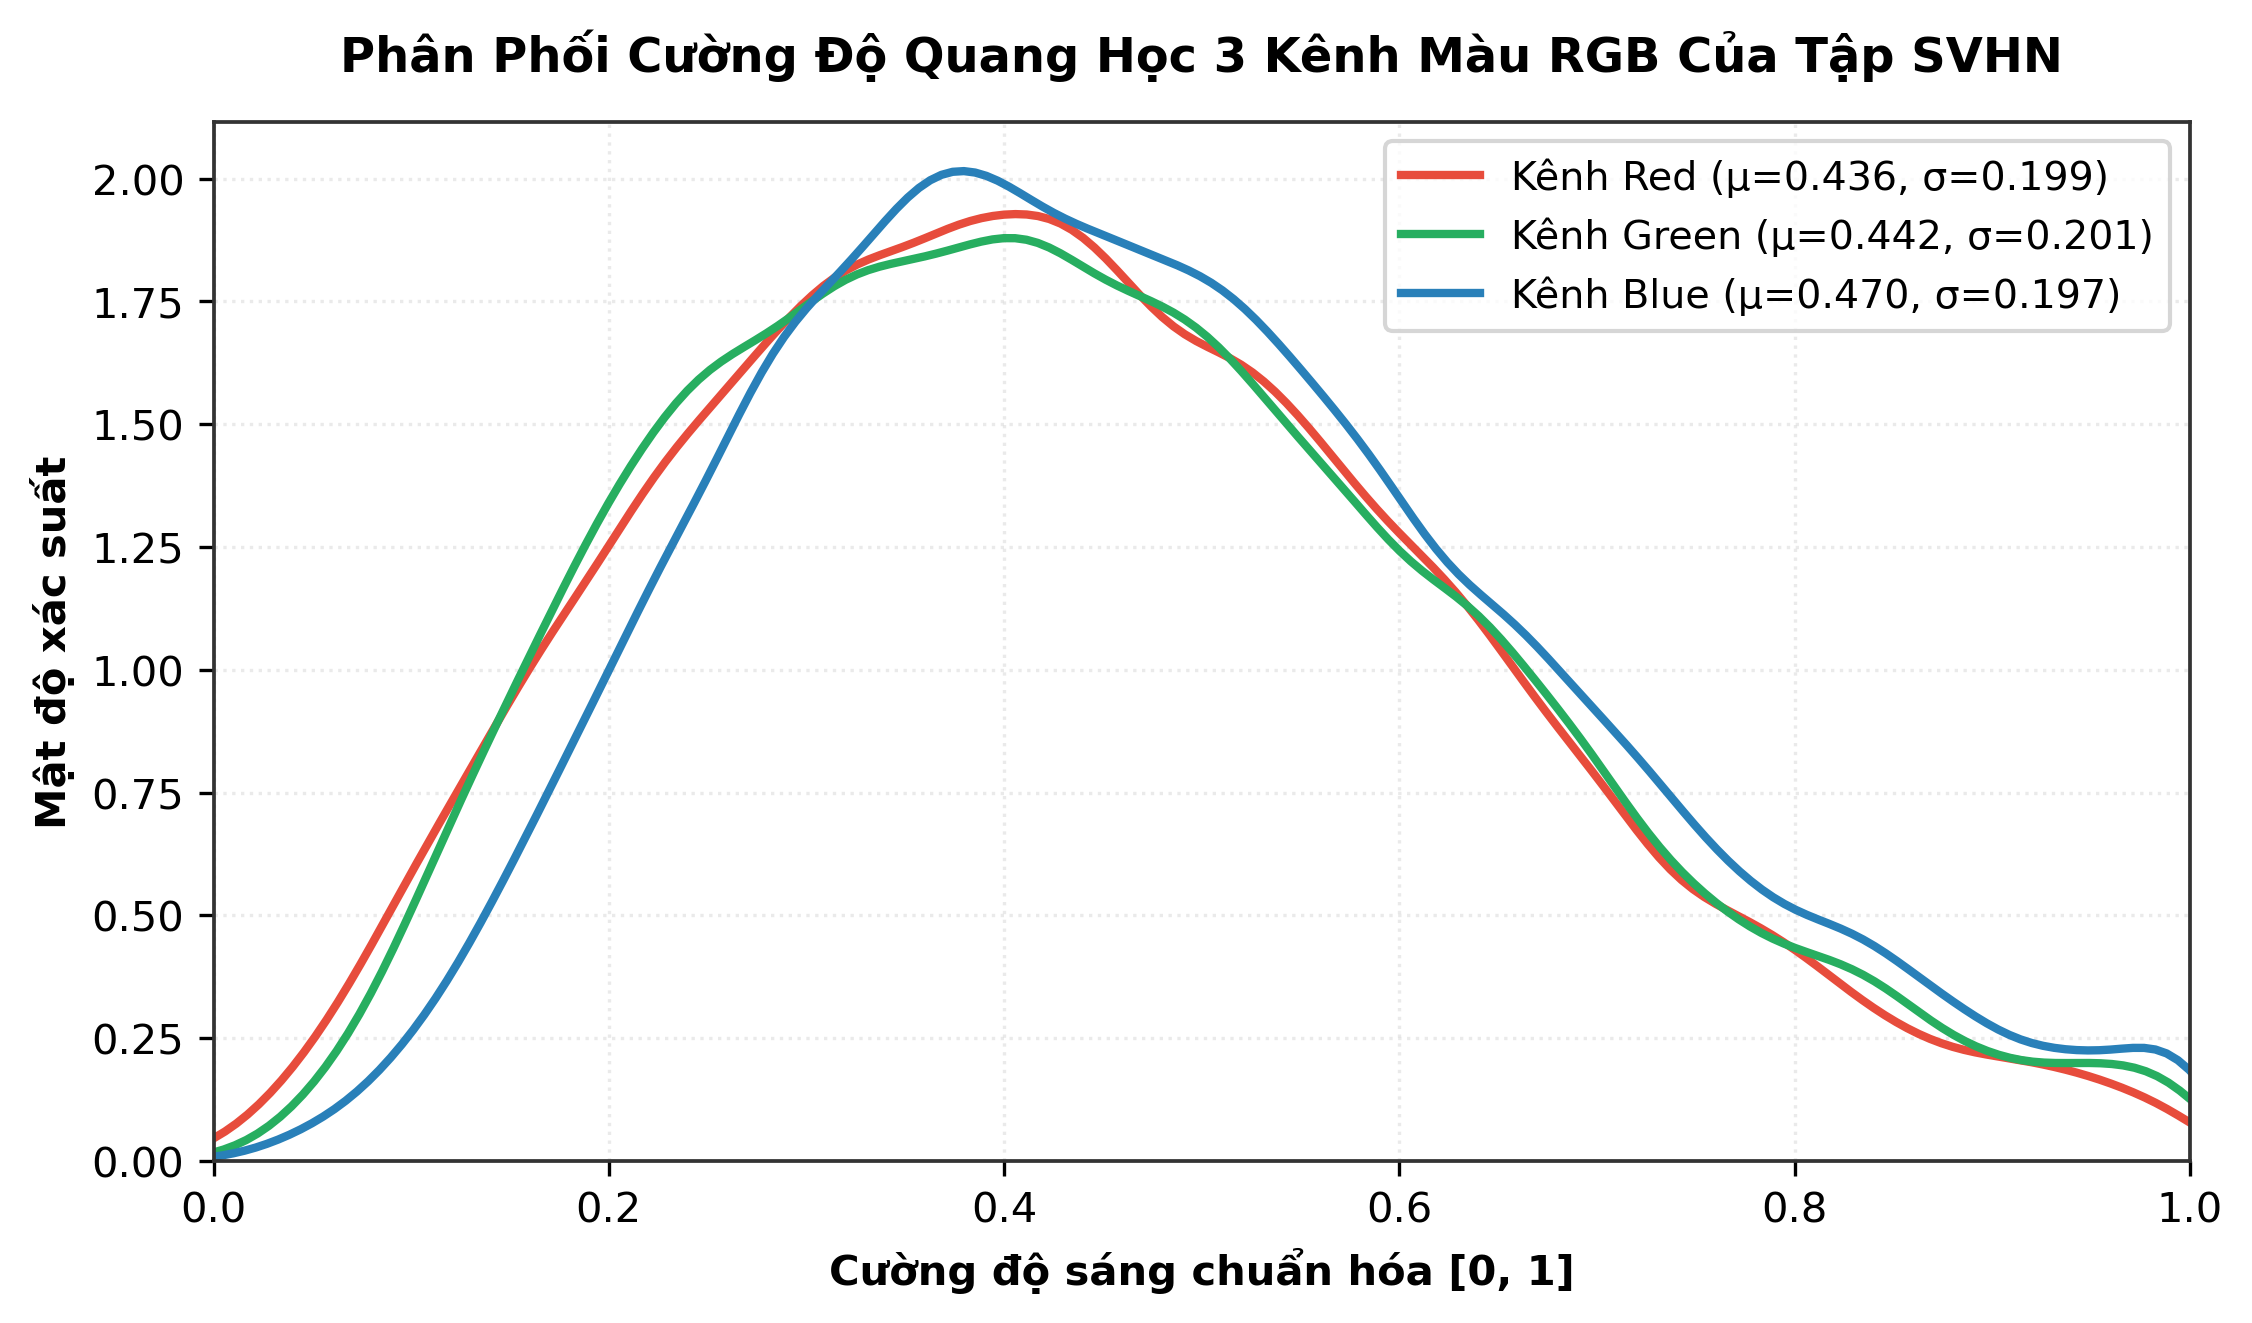
\includegraphics[width=0.80\textwidth]{images/fig406_svhn_rgb_channel_histograms.png}
    \caption{Phân phối mật độ quang học 3 kênh màu RGB của tập SVHN trên thang chuẩn hóa $[0, 1]$, làm rõ độ lệch phổ của kênh Blue.}
    \label{fig:svhn_rgb_channel_histograms}
\end{figure}

\textbf{Lưu ý chiến lược Data Augmentation cho SVHN:} Khác với phân loại ảnh đồ vật tổng quát, \textbf{tuyệt đối không áp dụng phép lật ngang ngẫu nhiên (\texttt{RandomHorizontalFlip})} cho SVHN. Việc lật ngang chữ số sẽ làm thay đổi bản chất hình học của ký tự (ví dụ số 2, 3, 5, 7 bị lật ngược trở thành ký tự vô nghĩa hoặc gây nhầm lẫn trầm trọng). Chiến lược tăng cường hợp lý cho SVHN là:
\begin{itemize}[leftmargin=*]
    \item \texttt{RandomCrop(32, padding=4)}: Dịch chuyển nhẹ tâm ảnh để mạng học cơ chế định vị không gian bất biến.
    \item \texttt{ColorJitter(brightness=0.1, contrast=0.1)}: Làm quen với chênh lệch cường độ sáng và độ tương phản tự nhiên ngoài trời.
\end{itemize}

\begin{lstlisting}[language=Python, caption={Pipeline xây dựng DataLoader và tăng cường dữ liệu đặc thù cho SVHN.}, label={lst:svhn_pipeline}]
import torchvision.datasets as dsets
import torchvision.transforms as transforms
from torch.utils.data import DataLoader

def get_svhn_dataloaders(data_dir="data", batch_size=64, num_workers=2):
    # Tham so chuan hoa kenh tinh toan tu buoc EDA
    svhn_mean = (0.435, 0.440, 0.469)
    svhn_std = (0.192, 0.193, 0.190)
    
    # Pipeline bien doi cho tap Huan luyen: Crop nhe, Jitter mau, KHONG LAT NGANG
    train_transform = transforms.Compose([
        transforms.RandomCrop(32, padding=4, padding_mode='edge'),
        transforms.ColorJitter(brightness=0.1, contrast=0.1),
        transforms.ToTensor(),
        transforms.Normalize(mean=svhn_mean, std=svhn_std)
    ])
    
    # Pipeline bien doi cho tap Kiem tra: Chi ToTensor va Normalize
    test_transform = transforms.Compose([
        transforms.ToTensor(),
        transforms.Normalize(mean=svhn_mean, std=svhn_std)
    ])
    
    train_dataset = dsets.SVHN(root=data_dir, split='train', download=False, transform=train_transform)
    test_dataset = dsets.SVHN(root=data_dir, split='test', download=False, transform=test_transform)
    
    train_loader = DataLoader(train_dataset, batch_size=batch_size, shuffle=True, 
                              num_workers=num_workers, pin_memory=True)
    test_loader = DataLoader(test_dataset, batch_size=batch_size, shuffle=False, 
                             num_workers=num_workers, pin_memory=True)
    
    return train_loader, test_loader
\end{lstlisting}

% =========================================================================
% 4.4. EUROSAT (SENTINEL-2 SATELLITE IMAGES)
% =========================================================================
\section{Khảo Sát, Phân Tích \& Chuẩn Hóa Bộ Dữ Liệu Ảnh Viễn Thám Vệ Tinh EuroSAT}

\subsection{Bản Chất Quang Phổ Viễn Thám \& Bài Toán Phân Loại Sử Dụng Đất (LULC)}
EuroSAT là bộ dữ liệu viễn thám chuẩn quốc tế được công bố bởi Viện Nghiên cứu Trí tuệ Nhân tạo Đức (DFKI) và Đại học Kaiserslautern (Helber et al., IEEE JSTARS 2019). Dữ liệu được trích xuất từ chùm vệ tinh quan sát Trái Đất Sentinel-2 thuộc chương trình không gian Copernicus của Liên minh Châu Âu (EU) và Cơ quan Vũ trụ Châu Âu (ESA).

Tập dữ liệu bao gồm $27,000$ ảnh viễn thám quang học RGB độ phân giải không gian cao ($10\,\text{m/pixel}$), kích thước chuẩn hóa $64 \times 64 \times 3$ điểm ảnh (Hình \ref{fig:eurosat_sample_grid}). Khác với ảnh chụp thông thường dưới mặt đất, ảnh viễn thám vệ tinh sở hữu những đặc trưng vật lý viễn thám độc đáo:
\begin{itemize}[leftmargin=*]
    \item \textbf{Góc nhìn thẳng đứng từ đỉnh đầu (Nadir Observation):} Ảnh được thu thập từ độ cao quỹ đạo khoảng $786\,\text{km}$, loại bỏ hoàn toàn hiện tượng biến dạng phối cảnh ngang của ống kính góc nghiêng, mang lại tính đối xứng quay hoàn toàn trong không gian 2D.
    \item \textbf{Cấu trúc kết cấu không gian đa quy mô (Multi-scale Spatial Texture):} Các phân lớp đất bề mặt thể hiện đặc trưng kết cấu rõ rệt: mạng lưới giao thông đường dài thẳng tắp (\texttt{Highway}), vùng dân cư ô bàn cờ (\texttt{Residential}), thảm thực vật tán lá rậm rạp (\texttt{Forest}) hoặc các vùng nước phản xạ quang phổ đặc thù (\texttt{River}, \texttt{SeaLake}).
    \item \textbf{Ứng dụng thực tiễn to lớn:} Đóng vai trò là bài toán then chốt trong giám sát biến đổi khí hậu, quản lý quy hoạch đô thị, cảnh báo lũ lụt và dự báo sản lượng nông nghiệp toàn cầu.
\end{itemize}

\begin{figure}[H]
    \centering
    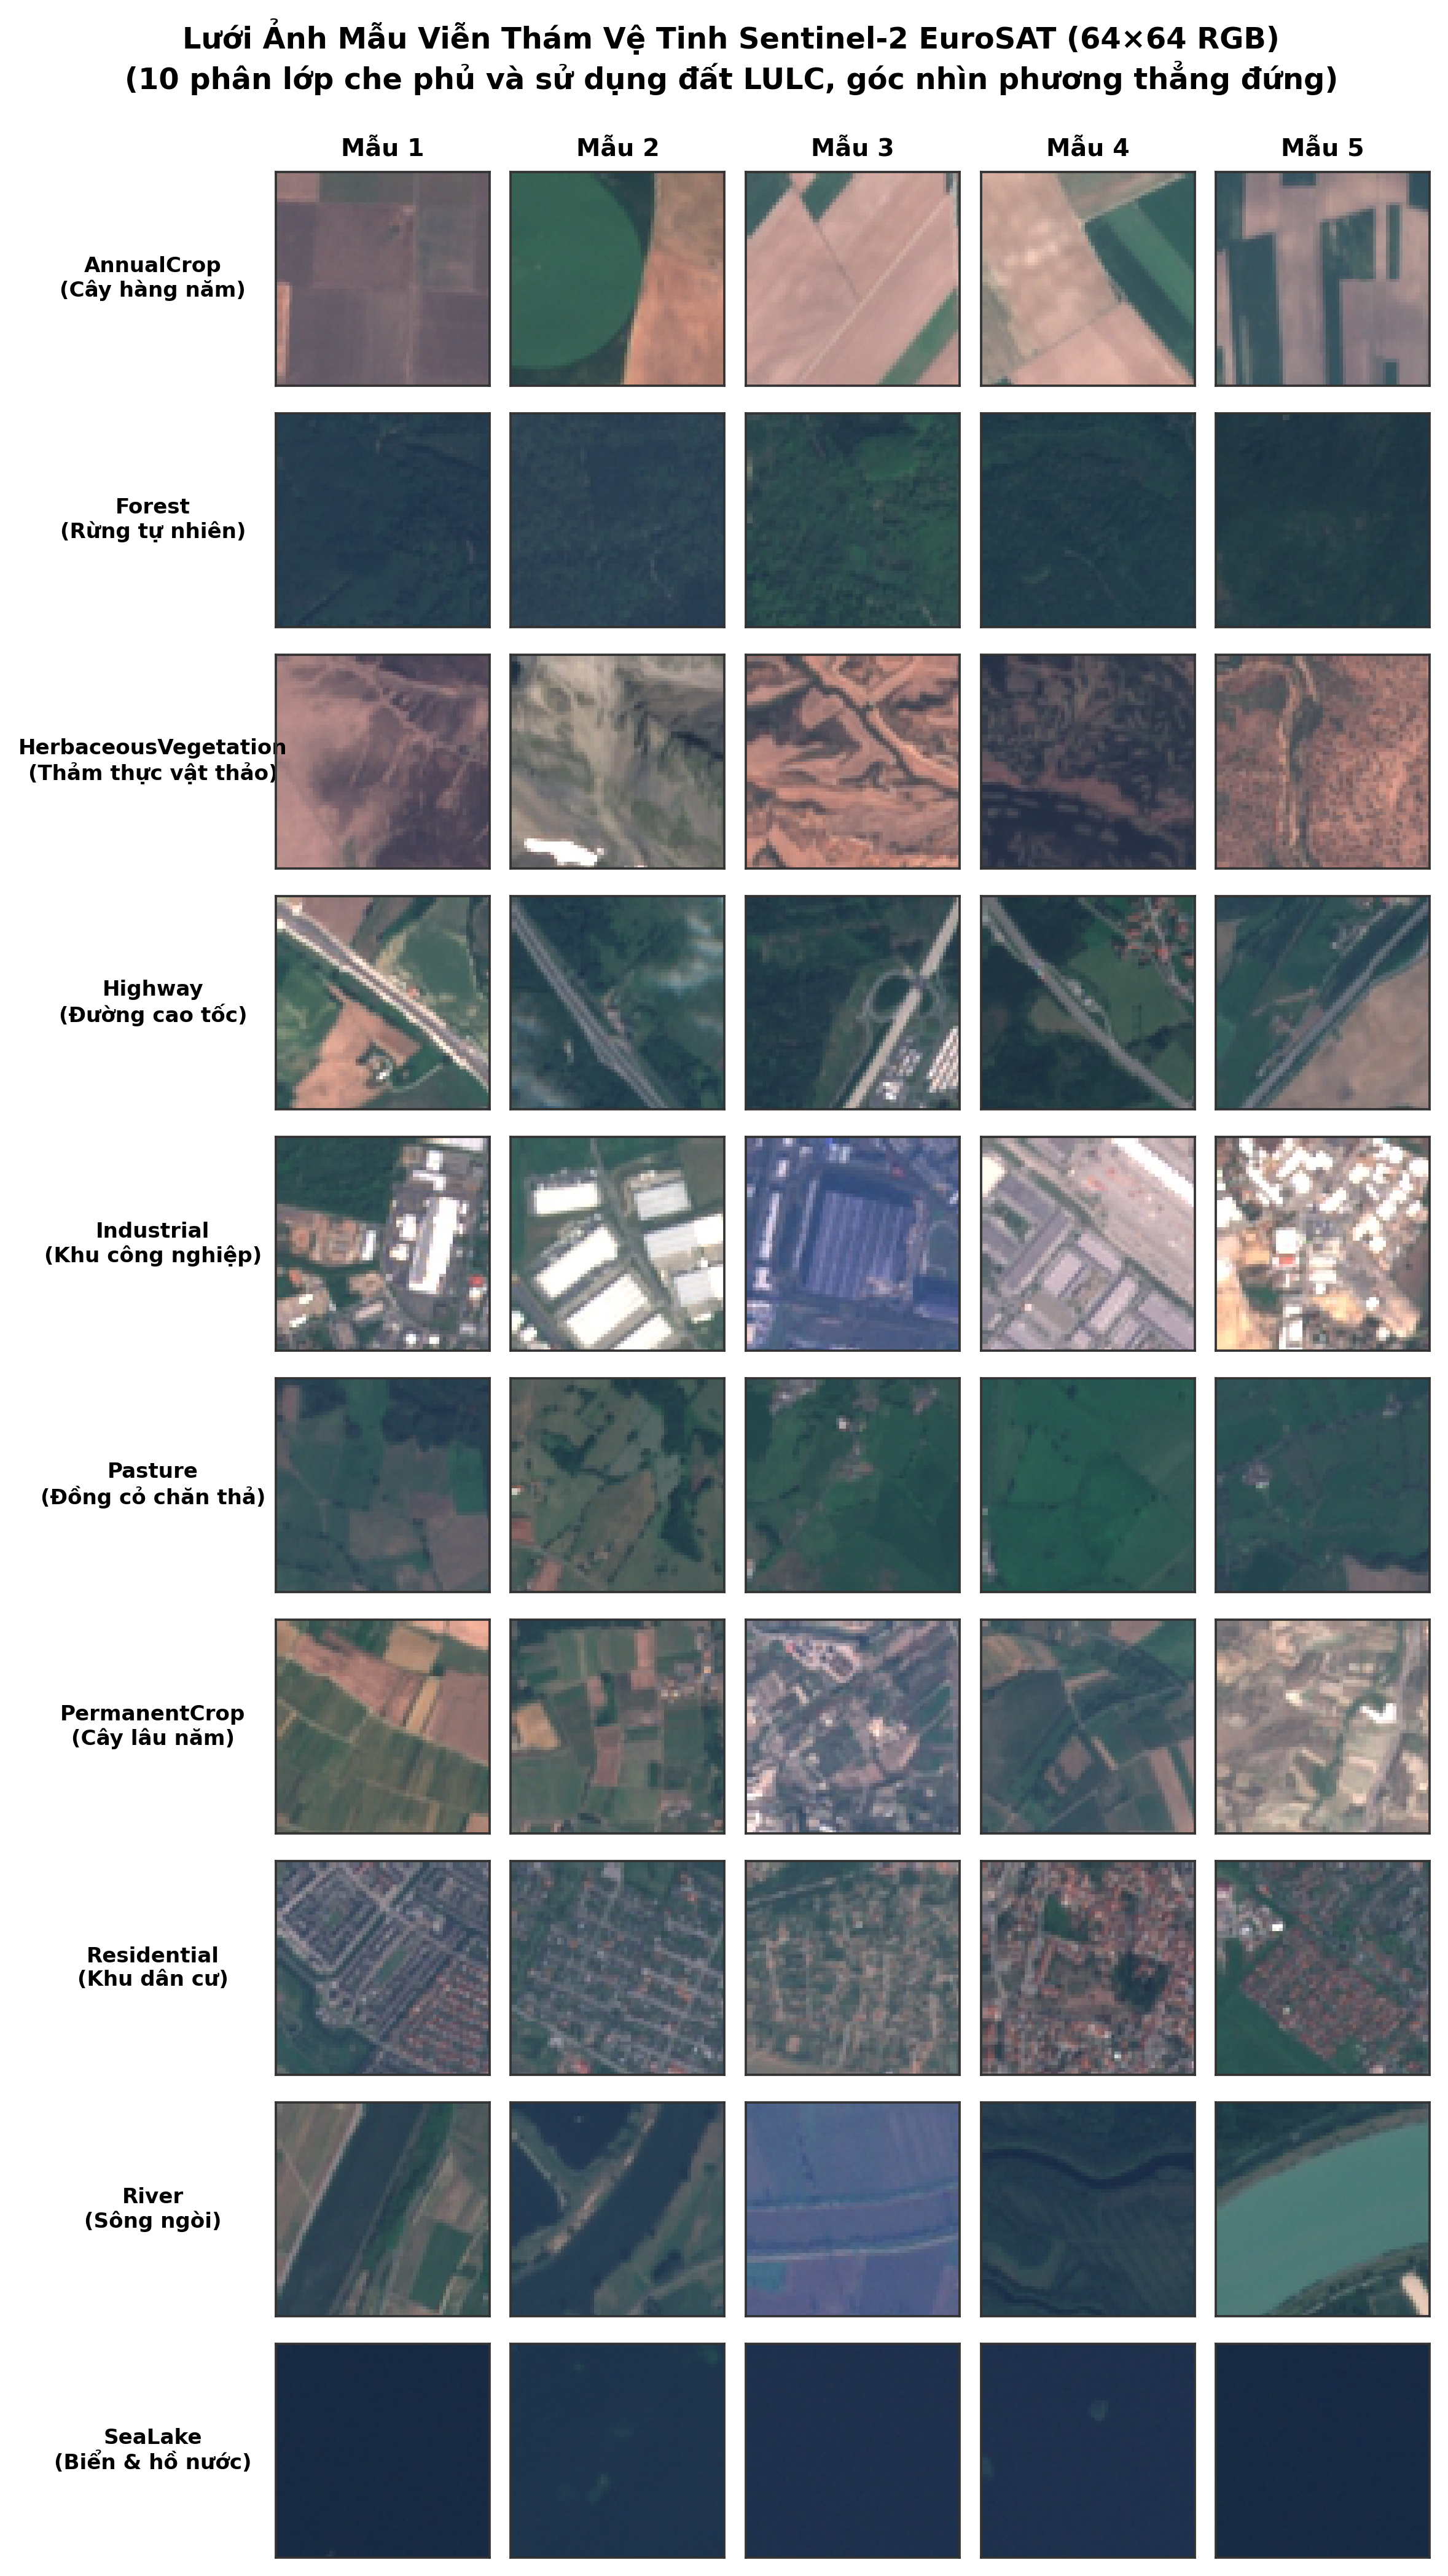
\includegraphics[width=0.78\textwidth]{images/fig407_eurosat_sample_grid.png}
    \caption{Lưới ảnh mẫu viễn thám vệ tinh Sentinel-2 EuroSAT ($64 \times 64 \times 3$ RGB) minh họa 10 phân lớp sử dụng và che phủ đất LULC quan sát từ quỹ đạo Trái Đất.}
    \label{fig:eurosat_sample_grid}
\end{figure}

\subsection{Hệ Thống 10 Phân Lớp LULC \& Cấu Trúc Phân Chia Dữ Liệu}
EuroSAT được phân chia thành \textbf{10 phân lớp bề mặt đất} với số lượng mẫu tương đối cân bằng từ $2,000$ đến $3,000$ ảnh mỗi lớp (Bảng \ref{tab:eurosat_stats} và Hình \ref{fig:eurosat_class_distribution}). Dữ liệu được phân chia phân tầng chuẩn với tỷ lệ $80\%$ Train ($21,600$ ảnh) và $20\%$ Test ($5,400$ ảnh).

\begin{table}[H]
\centering
\caption{Thống kê định lượng 10 phân lớp sử dụng và che phủ đất trong tập ảnh vệ tinh EuroSAT.}
\label{tab:eurosat_stats}
\small
\setlength{\tabcolsep}{4pt}
\begin{tabularx}{\textwidth}{clccX}
\toprule
\textbf{Mã} & \textbf{Tên Phân Lớp LULC} & \textbf{Số Mẫu} & \textbf{Tỷ Lệ} & \textbf{Đặc trưng phản xạ phổ \& Kết cấu không gian} \\
\midrule
0 & AnnualCrop (Cây trồng hàng năm)     & $3,000$ & $11.11\%$ & Đất canh tác nông nghiệp theo mùa, kết cấu luống kẻ sọc \\
1 & Forest (Rừng tự nhiên)               & $3,000$ & $11.11\%$ & Tán rừng rậm rạp, hấp thụ mạnh ánh sáng đỏ, màu xanh lục thẫm \\
2 & HerbaceousVegetation (Thực vật thảo)& $3,000$ & $11.11\%$ & Thảm cỏ tự nhiên, đầm lầy cạn, kết cấu mịn đồng nhất \\
3 & Highway (Đường cao tốc)              & $2,500$ & $9.26\%$  & Dải hẹp thẳng dài kéo dài cắt ngang địa hình, bề mặt bê tông \\
4 & Industrial (Khu công nghiệp)         & $2,500$ & $9.26\%$  & Cụm nhà xưởng mái tôn phẳng lớn, đường bãi xe, phản xạ cao \\
5 & Pasture (Đồng cỏ chăn thả)           & $2,000$ & $7.41\%$  & Bãi chăn thả gia súc nông thôn, màu xanh nhạt phân vùng ô nhỏ \\
6 & PermanentCrop (Cây lâu năm)         & $2,500$ & $9.26\%$  & Vườn cây ăn quả, đồn điền cây công nghiệp, hàng lối cây phân cấp \\
7 & Residential (Khu dân cư)             & $3,000$ & $11.11\%$ & Mái nhà ngói đỏ/xám xen kẽ đường nội bộ ô bàn cờ mật độ cao \\
8 & River (Sông ngòi)                    & $2,500$ & $9.26\%$  & Thủy vực dòng chảy tự nhiên uốn lượn, hấp thụ quang phổ mạnh \\
9 & SeaLake (Biển và hồ nước)            & $3,000$ & $11.11\%$ & Thủy vực tĩnh diện tích rộng, màu xanh lam đậm đến đen sẫm \\
\midrule
\multicolumn{2}{l}{\textbf{Tổng cộng toàn bộ mẫu}} & $\mathbf{27,000}$ & $\mathbf{100.0\%}$ & \textbf{Phân chia Train: 21,600 (80\%) / Test: 5,400 (20\%)} \\
\bottomrule
\end{tabularx}
\end{table}

\begin{figure}[H]
    \centering
    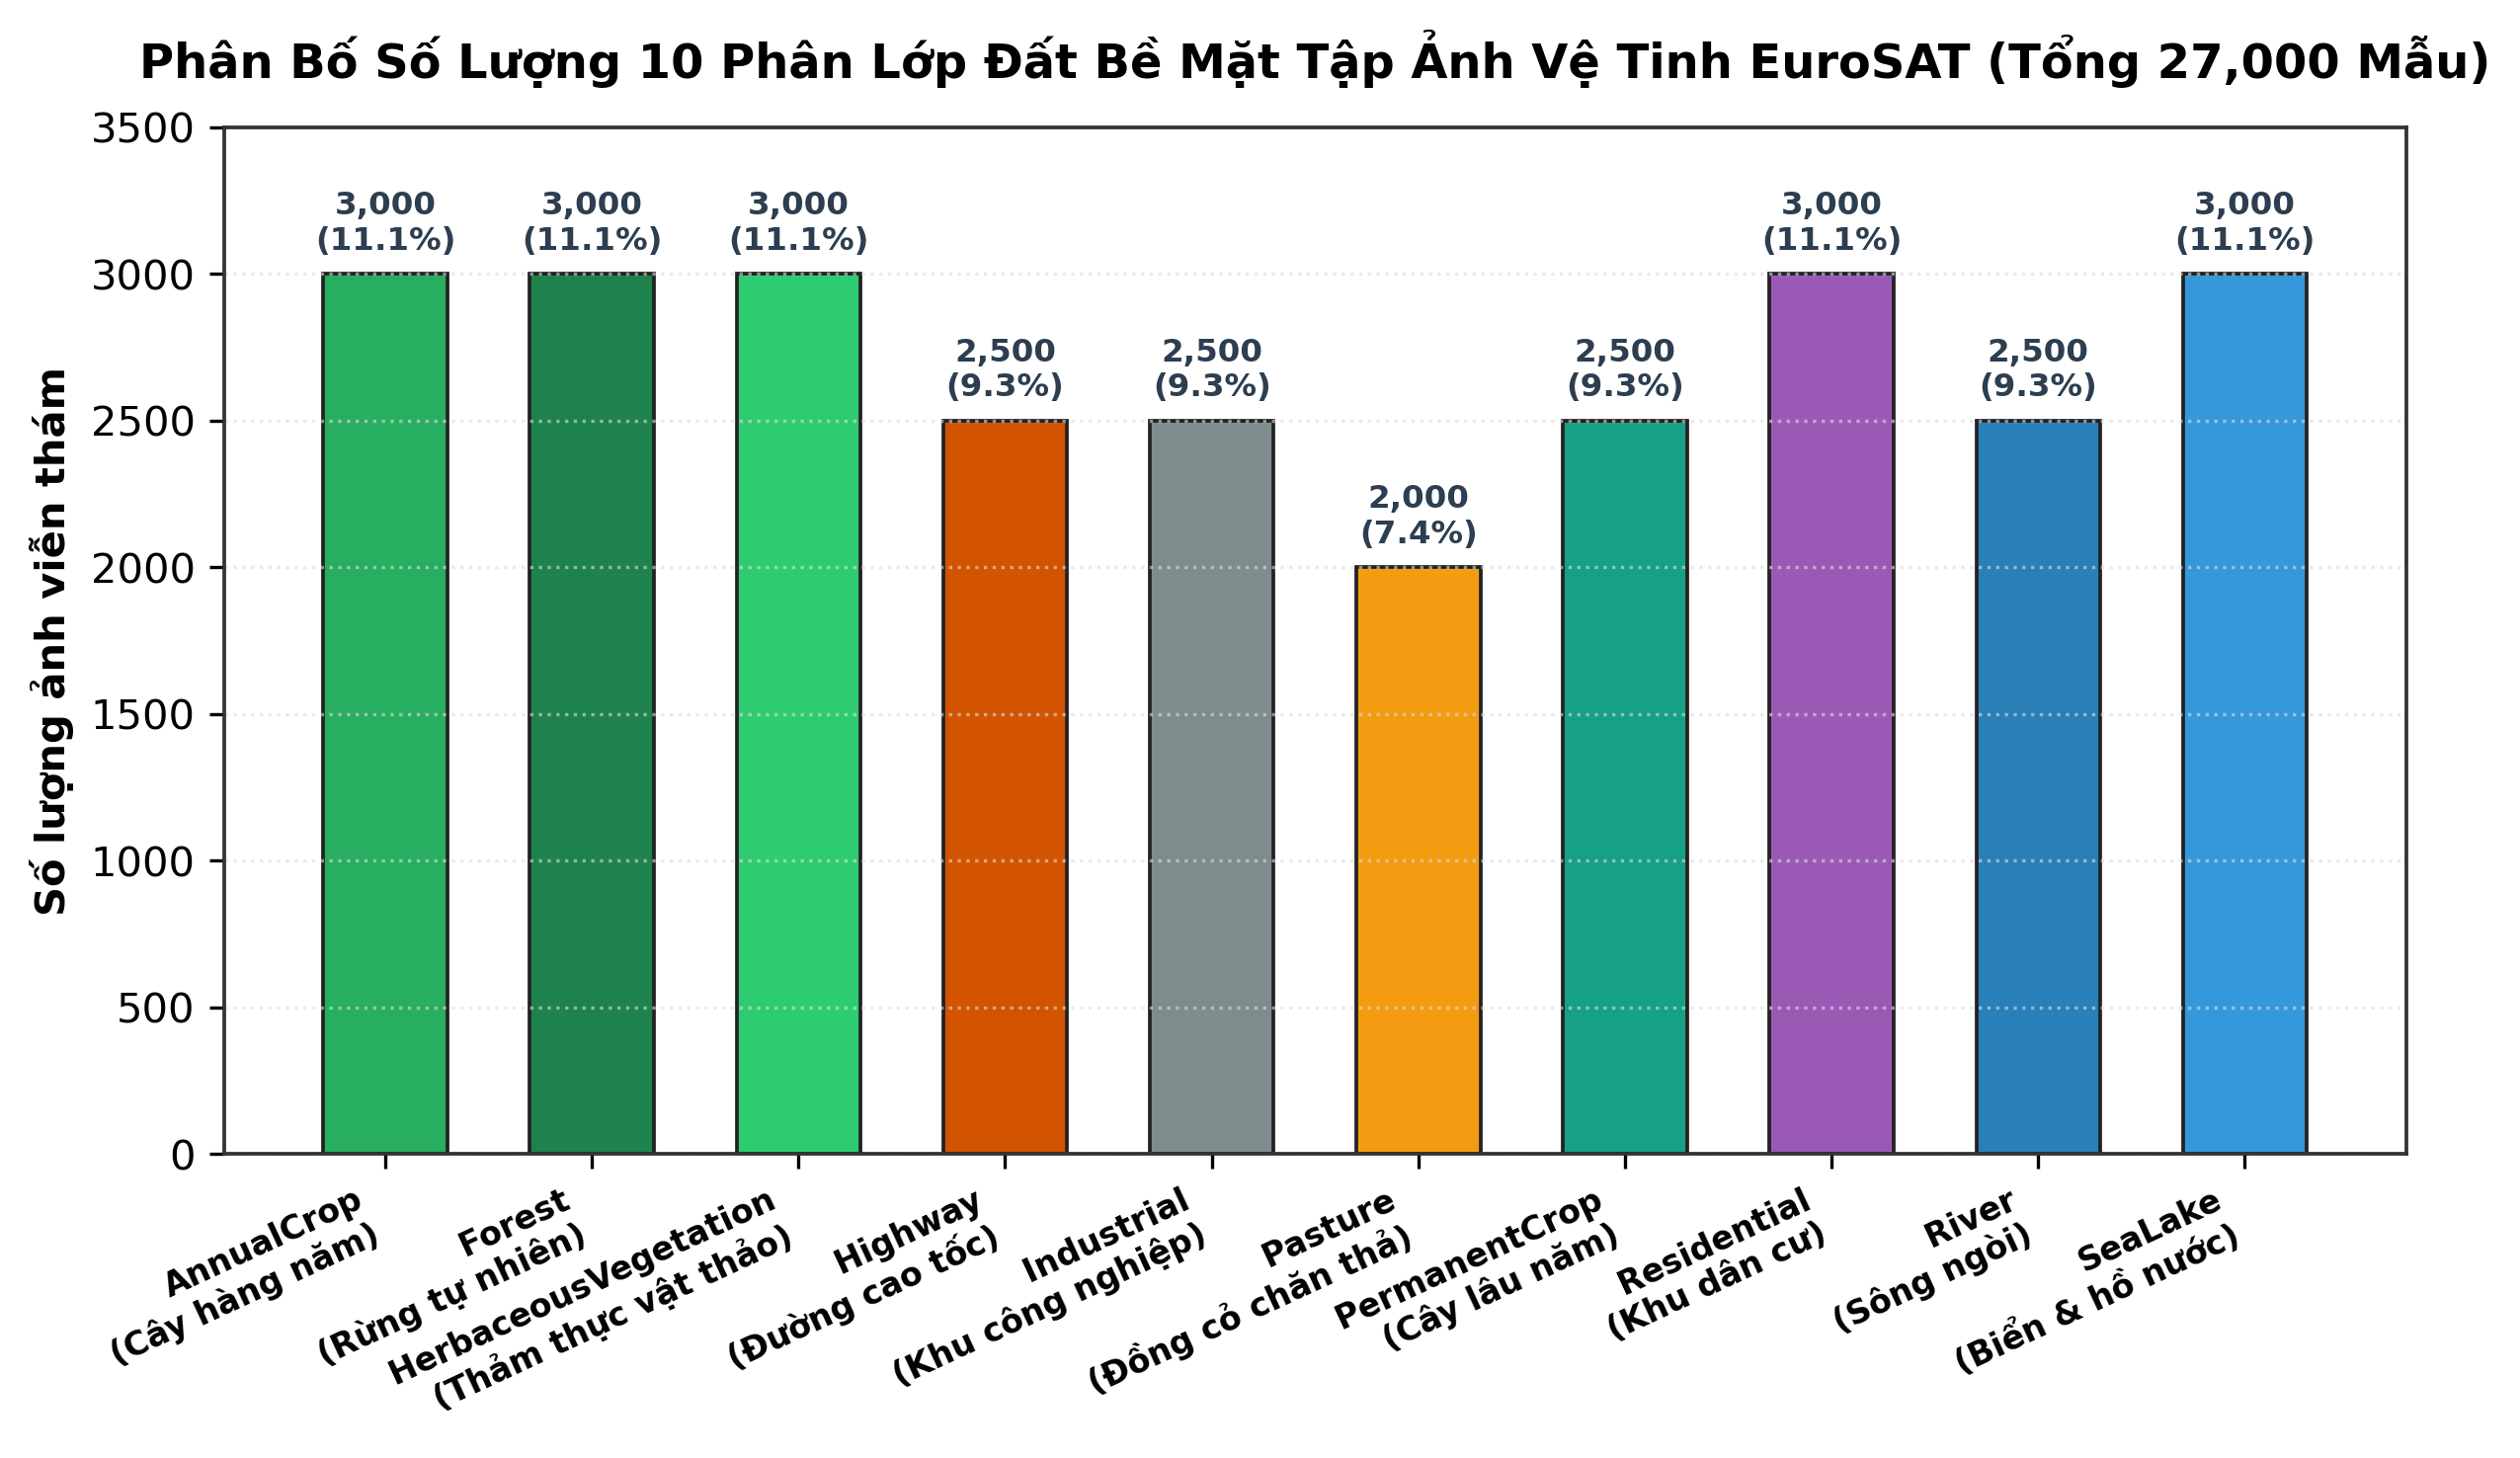
\includegraphics[width=0.88\textwidth]{images/fig408_eurosat_class_distribution.png}
    \caption{Phân bố số lượng và tỷ lệ phần trăm 10 phân lớp sử dụng và che phủ đất LULC trên tập ảnh vệ tinh EuroSAT (27,000 mẫu).}
    \label{fig:eurosat_class_distribution}
\end{figure}

\subsection{Đặc Tính Phổ Phản Xạ Quang Học \& Kỹ Thuật Tăng Cường Đối Xứng Đẳng Hướng 2D}
Phân tích Hình \ref{fig:eurosat_rgb_spectral_histograms} làm sáng tỏ các đặc tính phổ phản xạ quang học của ảnh viễn thám:
\begin{itemize}[leftmargin=*]
    \item Tham số quang học thực nghiệm chuẩn hóa trên dải $[0, 1]$ đạt:
    \begin{equation}
        \boldsymbol{\mu}_{\text{EuroSAT}} = [0.344, \, 0.380, \, 0.408], \quad \boldsymbol{\sigma}_{\text{EuroSAT}} = [0.093, \, 0.065, \, 0.054]
    \end{equation}
    \item Kênh Red ($\mu_R = 0.344$) có giá trị thấp nhất do diệp lục tố của thảm thực vật (\texttt{Forest}, \texttt{AnnualCrop}, \texttt{Pasture}) hấp thụ mạnh dải sóng đỏ ($665\,\text{nm}$) để phục vụ quang hợp. Kênh Blue ($\mu_B = 0.408$) có độ phản xạ trung bình cao nhất do tác động tán xạ khí quyển Rayleigh ở bước sóng ngắn và sự phản xạ của các công trình bê tông đô thị.
\end{itemize}

\begin{figure}[H]
    \centering
    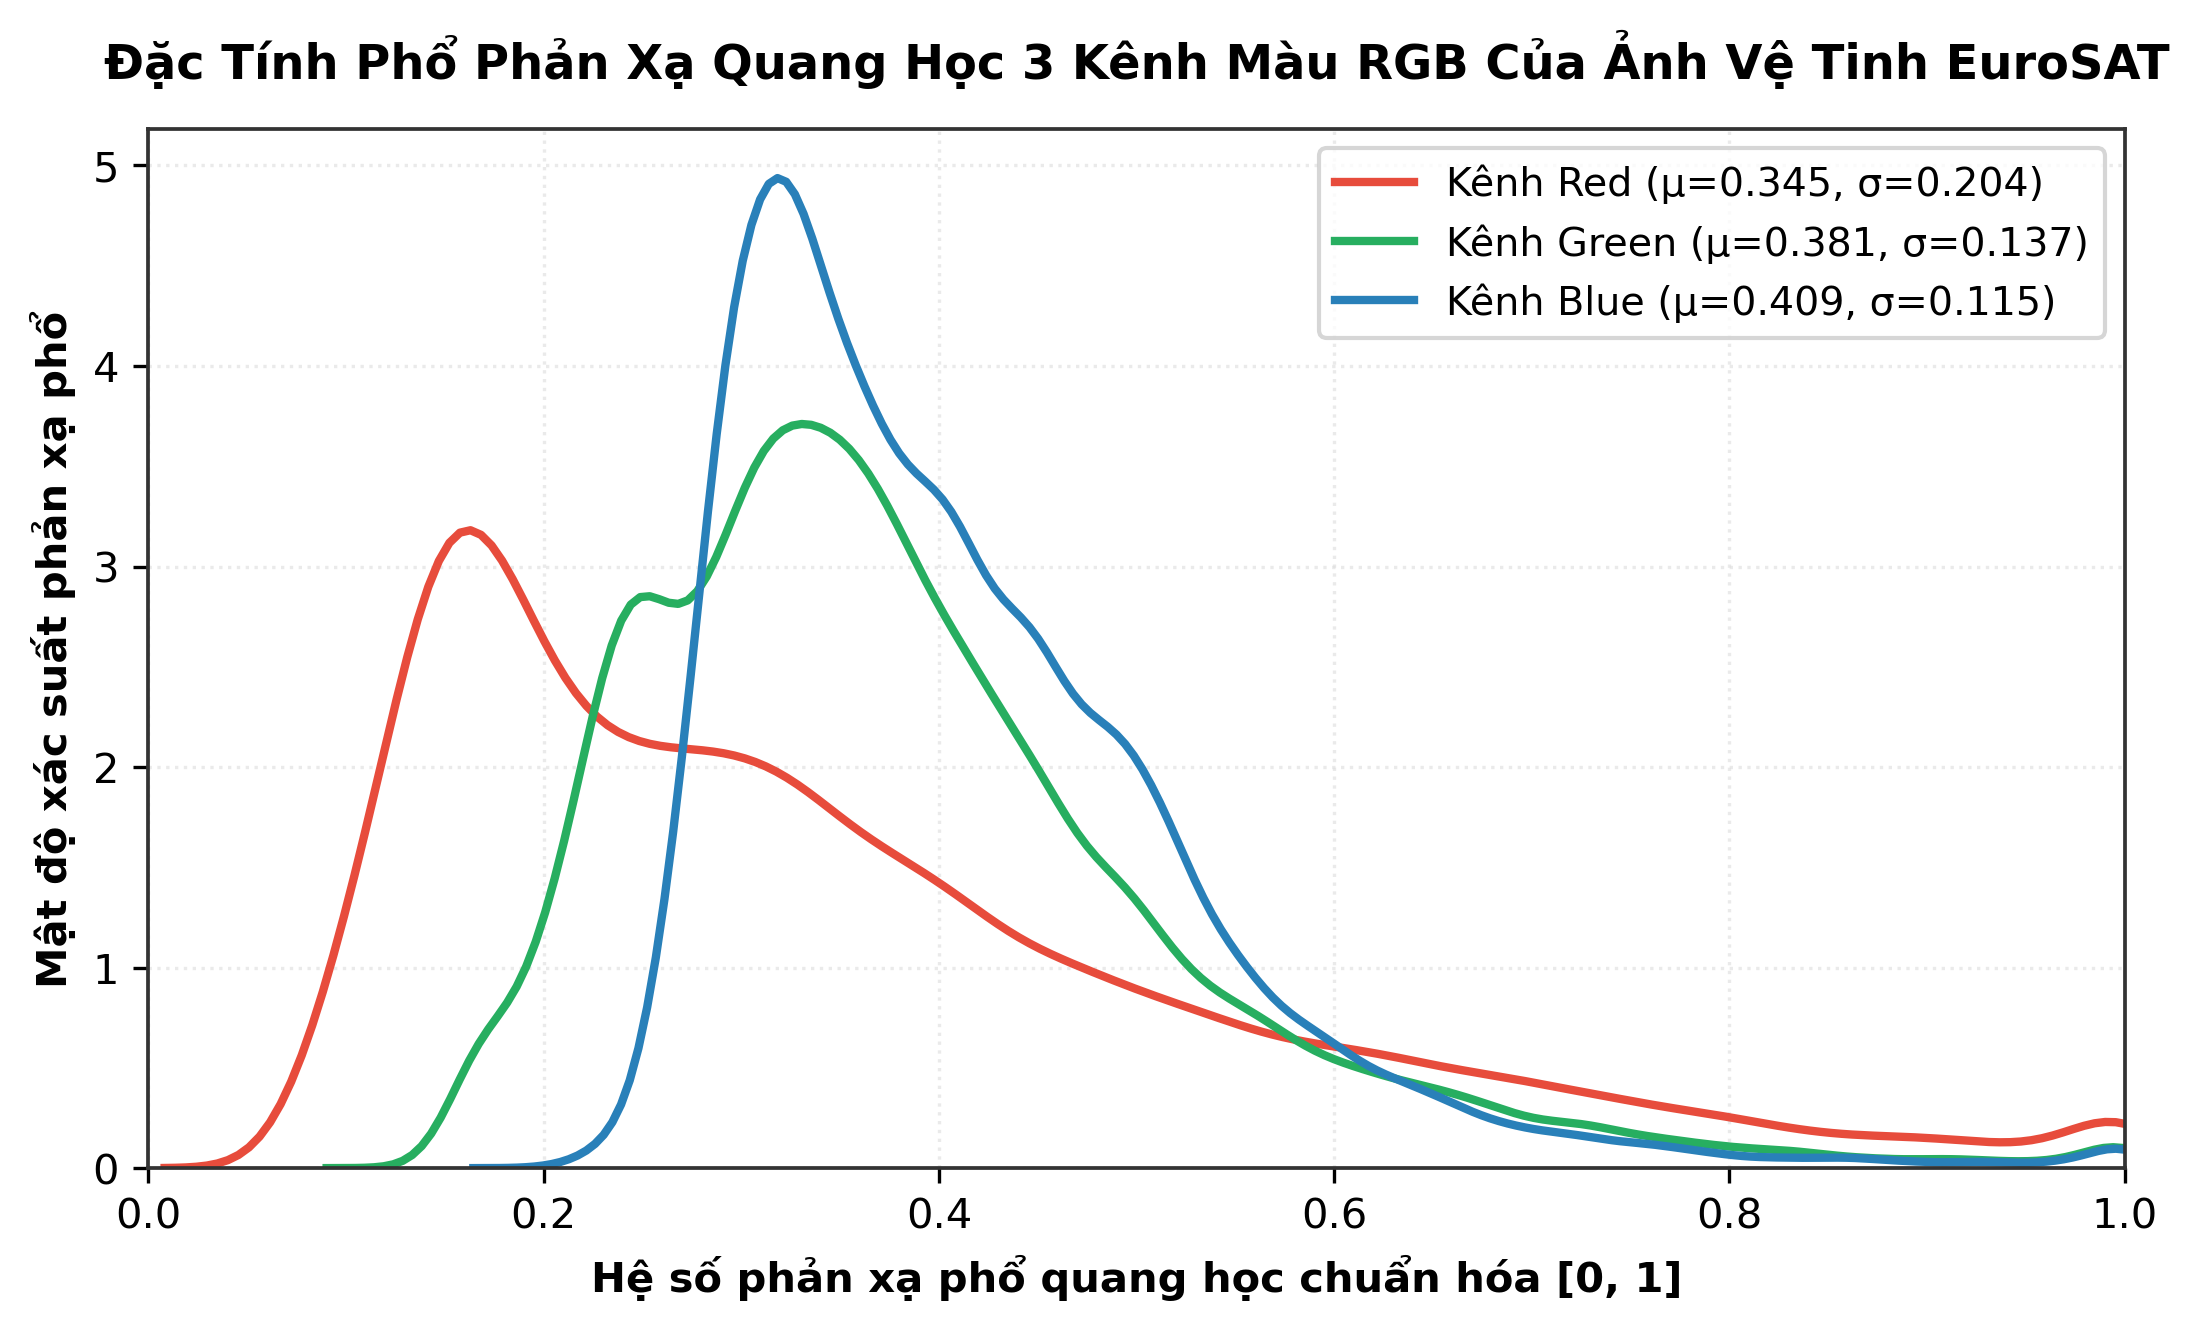
\includegraphics[width=0.80\textwidth]{images/fig409_eurosat_rgb_spectral_histograms.png}
    \caption{Đặc tính phổ phản xạ quang học 3 kênh màu RGB của ảnh viễn thám vệ tinh EuroSAT, thể hiện sự hấp thụ phổ đỏ của thảm thực vật.}
    \label{fig:eurosat_rgb_spectral_histograms}
\end{figure}

\textbf{Chiến lược Tăng cường Dữ liệu Đối Xứng Đẳng Hướng (Isotropic Augmentation):}
Khác hoàn toàn với chữ số SVHN vốn có chiều đọc cố định, các bức ảnh chụp vệ tinh nhìn thẳng góc từ trên cao không có khái niệm ``đầu trên'' hay ``đầu dưới''. Một cánh rừng, một dòng sông hay một khu công nghiệp khi xoay $90^\circ, 180^\circ$ hoặc lật gương vẫn giữ nguyên trọn vẹn bản chất phân loại địa lý:
\begin{itemize}[leftmargin=*]
    \item Áp dụng đồng thời \texttt{RandomHorizontalFlip(p=0.5)} và \texttt{RandomVerticalFlip(p=0.5)}.
    \item Áp dụng xoay ngẫu nhiên \texttt{RandomRotation(degrees=15)} để mô hình học được tính bất biến quay không gian hoàn chỉnh.
\end{itemize}

\begin{lstlisting}[language=Python, caption={Pipeline nạp EuroSAT, tăng cường đối xứng 2D và tạo DataLoader.}, label={lst:eurosat_pipeline}]
import torch
import torchvision.datasets as dsets
import torchvision.transforms as transforms
from torch.utils.data import Dataset, DataLoader, random_split

class SubsetEuroSAT(Dataset):
    def __init__(self, base_ds, indices, transform=None):
        self.base_ds = base_ds
        self.indices = indices
        self.transform = transform
        
    def __len__(self):
        return len(self.indices)
        
    def __getitem__(self, idx):
        img, label = self.base_ds[self.indices[idx]]
        if self.transform is not None:
            img = self.transform(img)
        return img, label

def get_eurosat_dataloaders(data_dir="data", batch_size=64, num_workers=2):
    # Tham so pho phan xa quang hoc EuroSAT
    euro_mean = (0.344, 0.380, 0.408)
    euro_std = (0.093, 0.065, 0.054)
    
    # Tang cuong dang huong 2D: Lat ngang, lat doc, quay tu do
    train_transform = transforms.Compose([
        transforms.RandomHorizontalFlip(p=0.5),
        transforms.RandomVerticalFlip(p=0.5),
        transforms.RandomRotation(degrees=15),
        transforms.ToTensor(),
        transforms.Normalize(mean=euro_mean, std=euro_std)
    ])
    
    test_transform = transforms.Compose([
        transforms.ToTensor(),
        transforms.Normalize(mean=euro_mean, std=euro_std)
    ])
    
    raw_ds = dsets.EuroSAT(root=data_dir, download=False)
    
    # Phan chia phan tang 80% Train, 20% Test
    generator = torch.Generator().manual_seed(42)
    train_size = int(0.8 * len(raw_ds))
    test_size = len(raw_ds) - train_size
    train_idx, test_idx = random_split(range(len(raw_ds)), [train_size, test_size], generator=generator)
    
    train_ds = SubsetEuroSAT(raw_ds, train_idx, transform=train_transform)
    test_ds = SubsetEuroSAT(raw_ds, test_idx, transform=test_transform)
    
    train_loader = DataLoader(train_ds, batch_size=batch_size, shuffle=True, 
                              num_workers=num_workers, pin_memory=True)
    test_loader = DataLoader(test_ds, batch_size=batch_size, shuffle=False, 
                             num_workers=num_workers, pin_memory=True)
    
    return train_loader, test_loader
\end{lstlisting}

% =========================================================================
% 4.5. DOI CHUAN TONG HOP
% =========================================================================
\section{Tổng Hợp Đối Chuẩn Cấu Trúc 3 Bộ Dữ Liệu \& Ma Trận Thiết Kế Mạng Nơ-ron}

\subsection{Bảng Đối Chuẩn Đa Chiều Giữa 3 Không Gian Dữ Liệu}
Hình \ref{fig:multidomain_tensor_matrix} và Bảng \ref{tab:multi_domain_benchmark} tổng hợp toàn diện các chỉ số kỹ thuật, định dạng tensor đầu vào, tính chất vật lý và chiến lược xử lý dữ liệu giữa 3 bộ dữ liệu đã khảo sát.

\begin{figure}[H]
    \centering
    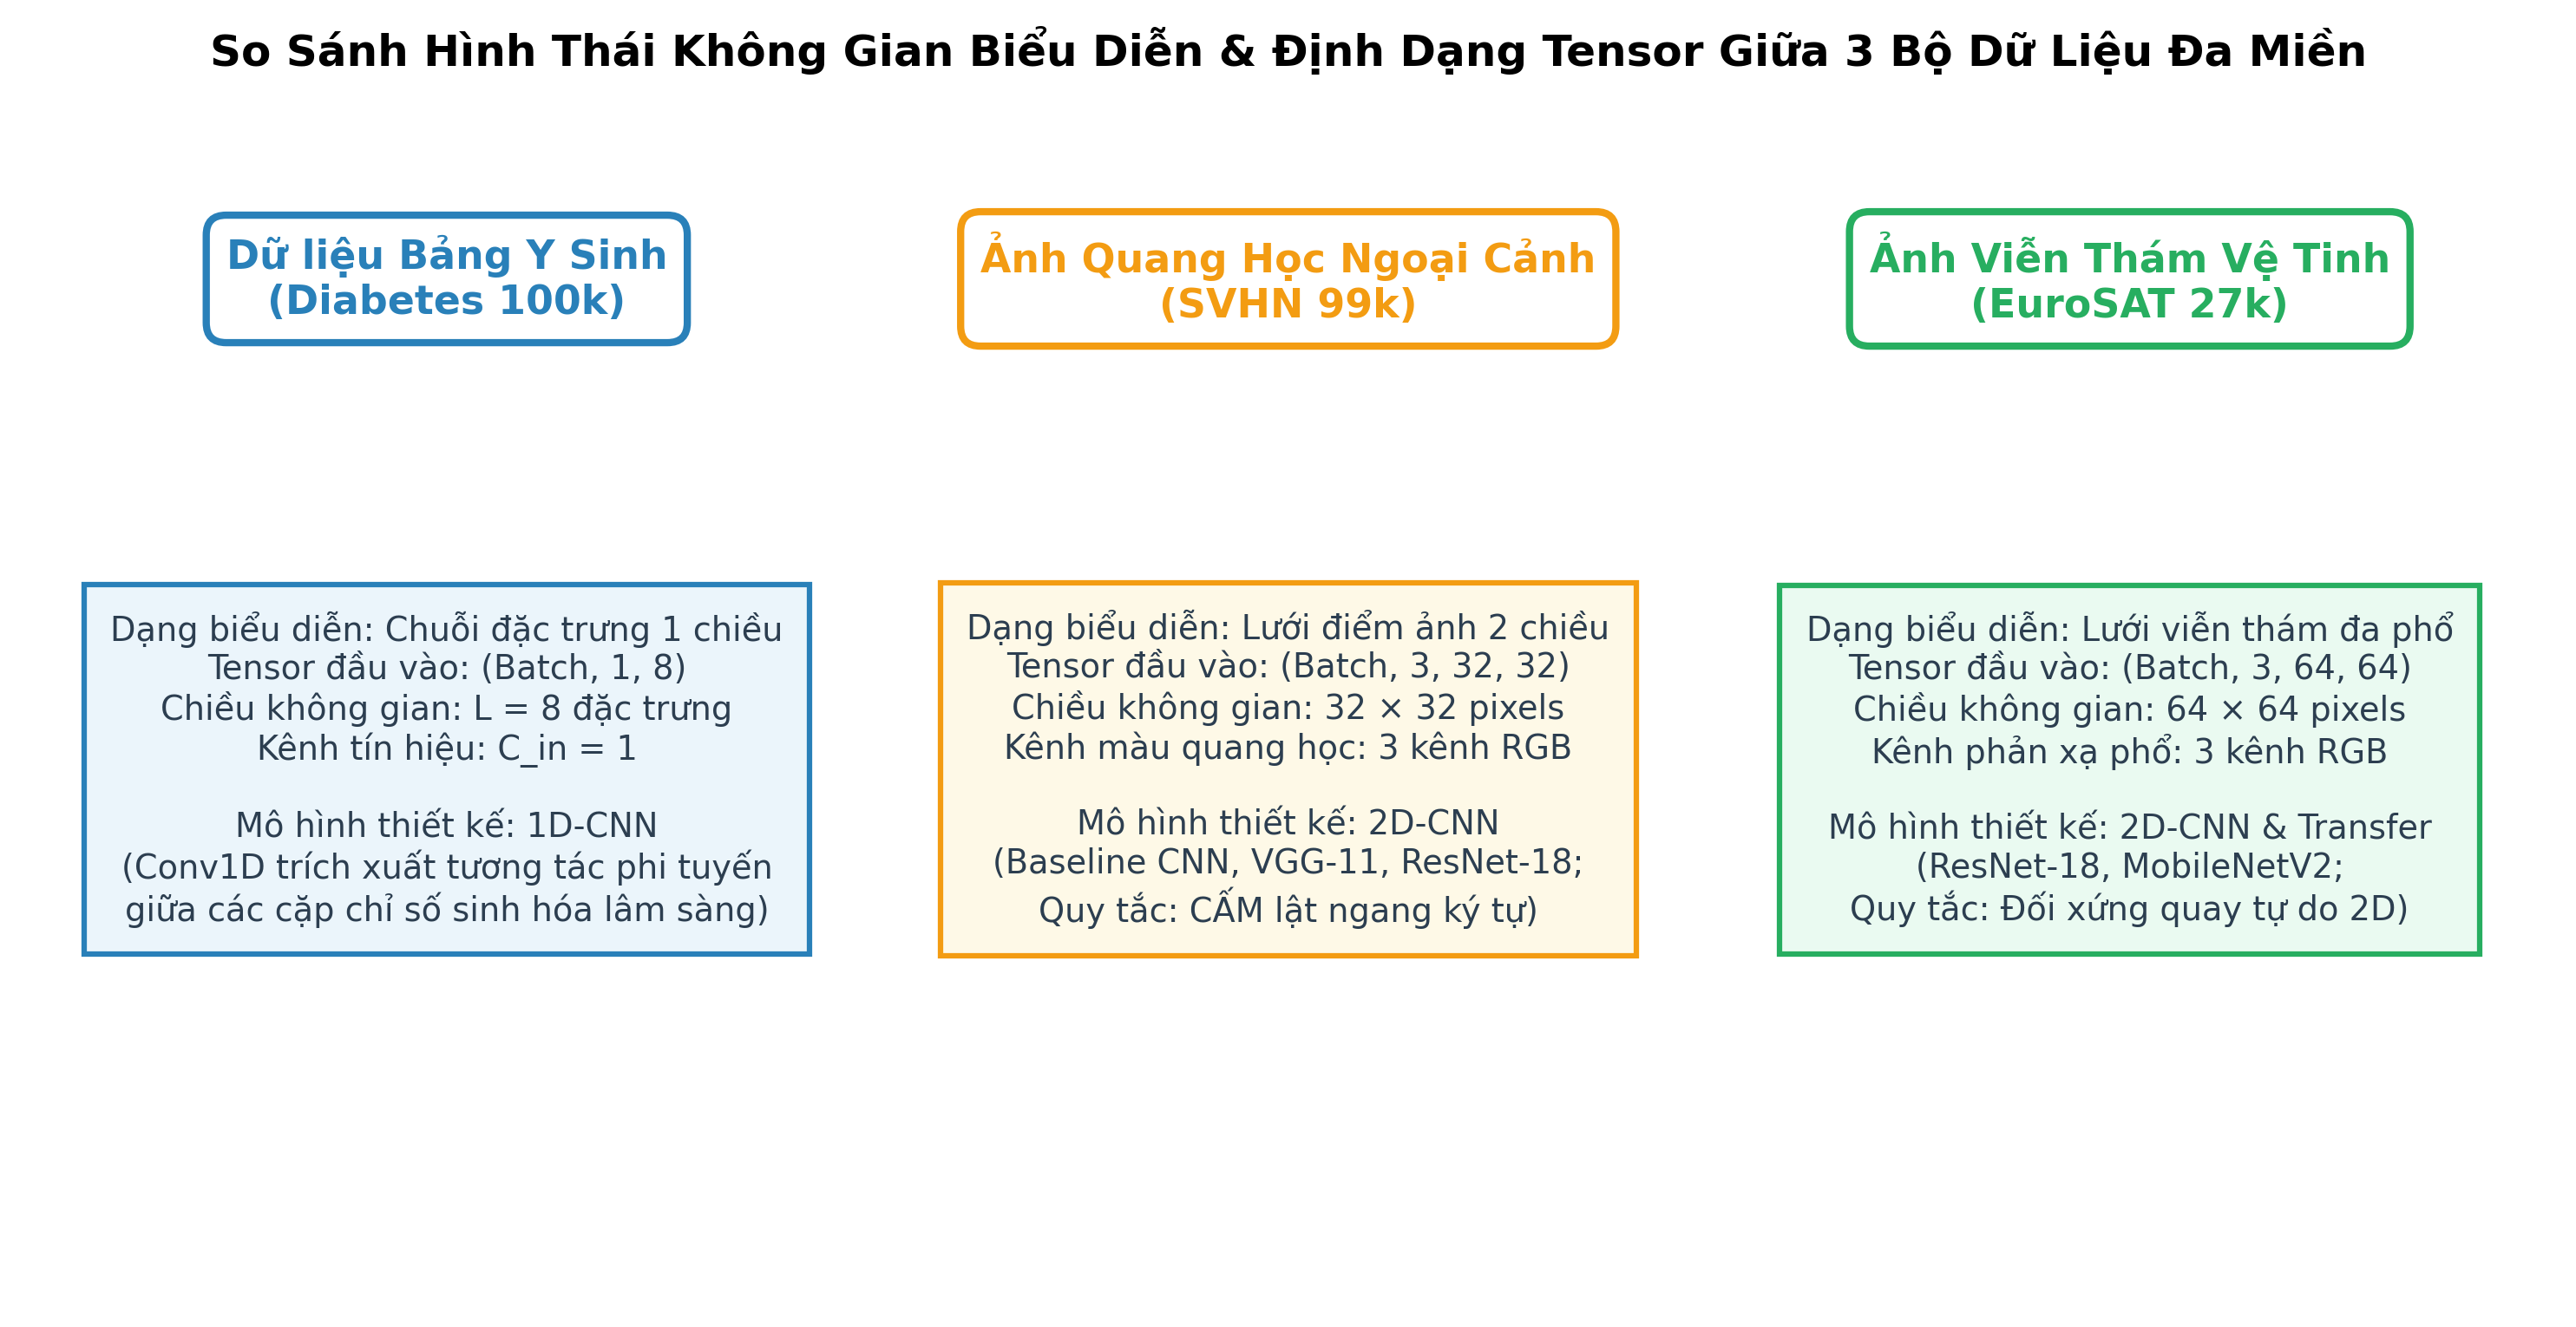
\includegraphics[width=0.92\textwidth]{images/fig410_multidomain_tensor_matrix.png}
    \caption{Sơ đồ so sánh hình thái không gian biểu diễn, cấu trúc tensor đầu vào và định hướng thiết kế mô hình giữa 3 bộ dữ liệu đa miền.}
    \label{fig:multidomain_tensor_matrix}
\end{figure}

\begin{table}[H]
\centering
\caption{Ma trận đối chuẩn cấu trúc đa miền giữa Diabetes, SVHN và EuroSAT.}
\label{tab:multi_domain_benchmark}
\small
\begin{tabularx}{\textwidth}{lXXX}
\toprule
\textbf{Tiêu chí Đối chuẩn} & \textbf{Diabetes Prediction (100k)} & \textbf{Street View HN (SVHN)} & \textbf{Sentinel-2 EuroSAT} \\
\midrule
\textbf{Miền dữ liệu} & Bảng Y Sinh (Tabular) & Ảnh Ngoại cảnh Tự nhiên & Ảnh Viễn thám Vệ tinh \\
\textbf{Kích thước đầu vào} & Tensor 1D: $(1, 8)$ & Tensor 2D: $3 \times 32 \times 32$ & Tensor 2D: $3 \times 64 \times 64$ \\
\textbf{Quy mô mẫu tổng} & $100,000$ hồ sơ ($96,128$ sạch) & $99,289$ ảnh màu & $27,000$ ảnh màu \\
\textbf{Cấu trúc phân chia} & Train: $76,902$ / Test: $19,226$ & Train: $73,257$ / Test: $26,032$ & Train: $21,600$ / Test: $5,400$ \\
\textbf{Số lớp mục tiêu} & $2$ lớp ($91.2\%$ âm, $8.8\%$ dương) & $10$ chữ số ($0 \to 9$) & $10$ phân lớp LULC đất bề mặt \\
\textbf{Thách thức cốt lõi} & Mất cân bằng lớp $10.4:1$, đặc trưng phân loại + sinh hóa & Nhiễu nền đô thị, chữ số lân cận xâm lấn, ngược sáng & Kết cấu bề mặt phức tạp, ranh giới thảm phủ tinh vi \\
\textbf{Chiến lược Chuẩn hóa} & StandardScaler (fit trên Train) & Channel Mean/Std $(0.435, 0.440, 0.469)$ & Channel Mean/Std $(0.344, 0.380, 0.408)$ \\
\textbf{Quy tắc Augmentation} & Không áp dụng & RandomCrop, ColorJitter; \textbf{cấm lật ngang} & RandomHorizontalFlip, RandomVerticalFlip, Rotation \\
\textbf{Kiến trúc tương thích} & 1D-CNN (Mạng tích chập 1 chiều) & Baseline CNN, VGG-11, ResNet-18 & ResNet-18, MobileNetV2, Transfer Learning \\
\bottomrule
\end{tabularx}
\end{table}

\subsection{Luận Giải Ma Trận Thiết Kế Kiến Trúc Học Sâu}
Từ kết quả đối chuẩn tại Bảng \ref{tab:multi_domain_benchmark}, chúng tôi xác lập các quyết định thiết kế mô hình:
\begin{itemize}[leftmargin=*]
    \item \textbf{Đối với dữ liệu bảng Diabetes:} Với quy mô lớn $96,128$ mẫu sau làm sạch và 8 đặc trưng lâm sàng, dữ liệu sở hữu độ sâu biểu diễn vượt trội so với các tập bảng nhỏ. Mô hình được lựa chọn là mạng tích chập 1 chiều (\textbf{1D-CNN}) với các khối Conv1D, BatchNorm1d và Adaptive Pooling để trích xuất tương tác phi tuyến cục bộ giữa các cặp chỉ số sinh hóa mà không bị giới hạn bởi tính độc lập tuyến tính.
    \item \textbf{Đối với ảnh ngoại cảnh SVHN:} Với kích thước $32 \times 32$ và dung lượng mẫu dồi dào ($>73,000$ mẫu train), mạng CNN cần có trường tiếp nhận (Receptive Field) đủ rộng để bao quát toàn bộ ô số mà không bị đánh lừa bởi chữ số lân cận. Các kiến trúc phù hợp bao gồm Baseline CNN (3 khối tích chập), VGG-11 (tập trung học biểu diễn hình học phân cấp) và ResNet-18.
    \item \textbf{Đối với ảnh viễn thám EuroSAT:} Độ phân giải $64 \times 64$ cùng kết cấu không gian phức tạp của 10 phân lớp địa lý đòi hỏi các mạng có khả năng học biểu diễn sâu và đa quy mô. ResNet-18 (với cơ chế Residual Learning) và MobileNetV2 (với Inverted Residual Block) kết hợp kỹ thuật Transfer Learning là những ứng viên xuất sắc nhất để đạt độ chính xác tối ưu trên miền dữ liệu viễn thám.
\end{itemize}

% =========================================================================
% 4.6. TÓM TẮT CHƯƠNG 4
% =========================================================================
\section{Tóm Tắt Chương 4}
Chương 4 đã hoàn thành toàn diện, bài bản và chuyên sâu quy trình khảo sát thực nghiệm, khám phá dữ liệu (EDA), kiểm toán sinh lý và thiết lập pipeline tiền xử lý trên 3 bộ dữ liệu đa miền:
\begin{itemize}[leftmargin=*]
    \item \textbf{Kiểm toán y sinh \& Chuẩn hóa tập Diabetes 100k cho 1D-CNN:} Xử lý tập dữ liệu lớn $100,000$ hồ sơ bệnh nhân; loại bỏ $3,854$ bản ghi trùng lặp và chuẩn hóa nhãn giới tính; phân tích sâu hai chỉ số sinh hóa chủ đạo (\texttt{HbA1c\_level} $r=0.41$ và \texttt{blood\_glucose\_level} $r=0.42$) tách biệt rõ rệt theo ngưỡng chẩn đoán lâm sàng $6.5\%$; đóng gói luồng dữ liệu tensor 1D $(N, 1, 8)$ chuyên biệt cho mạng tích chập 1 chiều.
    \item \textbf{Giải mã quang học tập ảnh ngoại cảnh SVHN:} Phân tích $99,289$ ảnh số nhà thực tế; định lượng hiện tượng mất cân bằng lớp tự nhiên (chữ số 1 chiếm $18.92\%$, số 9 chiếm $6.36\%$); trích xuất chuẩn xác tham số chuẩn hóa 3 kênh màu và xác lập quy tắc cấm lật ngang dữ liệu.
    \item \textbf{Khám phá viễn thám tập ảnh vệ tinh EuroSAT (Sentinel-2):} Khảo sát $27,000$ ảnh viễn thám của 10 phân lớp sử dụng và che phủ đất; bóc tách đặc tính hấp thụ phổ đỏ của thảm thực vật ($\mu_R = 0.344$); xây dựng chiến lược tăng cường dữ liệu đẳng hướng đối xứng hoàn toàn trong không gian 2D.
    \item \textbf{Đóng gói Pipeline PyTorch \& Thiết lập Ma Trận Kiến Trúc:} Hoàn thiện 3 hàm nạp dữ liệu chuẩn tắc, sinh các luồng \texttt{DataLoader} song song tối ưu hóa bộ nhớ GPU (\texttt{pin\_memory=True}), thiết lập ma trận đối chuẩn đa chiều làm bàn đạp vững chắc để bước sang Chương 5: Triển khai huấn luyện thực nghiệm và đối chuẩn 4 kiến trúc CNN.
\end{itemize}


% =========================================================================
% CHƯƠNG 5: HIỆN THỰC HÓA HUẤN LUYỆN THỰC NGHIỆM, ĐÁNH GIÁ & ĐỐI CHUẨN 4 KIẾN TRÚC CNN TRÊN 3 BỘ DỮ LIỆU ĐA MIỀN
% =========================================================================
% =========================================================================
% CHƯƠNG 5: HUẤN LUYỆN THỰC NGHIỆM VÀ ĐÁNH GIÁ 4 KIẾN TRÚC CNN TRÊN 3 BỘ DỮ LIỆU
% =========================================================================
\chapter{Huấn Luyện Thực Nghiệm \& Đánh Giá Các Kiến Trúc CNN Trên 3 Bộ Dữ Liệu}
\label{chap:chapter5_cnn_training_benchmarks}

Chương này trình bày việc cài đặt, huấn luyện thực nghiệm và đánh giá so sánh các mô hình mạng nơ-ron tích chập trên 3 bộ dữ liệu:
\begin{itemize}[leftmargin=*]
    \item \textbf{Dữ liệu bảng y sinh (Diabetes 100k):} Sử dụng mạng tích chập 1 chiều (\textbf{1D-CNN}) để dự đoán nguy cơ đái tháo đường dựa trên 8 chỉ số lâm sàng.
    \item \textbf{Dữ liệu ảnh ngoại cảnh (SVHN 99k):} Nhận diện 10 chữ số từ 0 đến 9 trên ảnh số nhà thực tế bằng 4 kiến trúc: Baseline CNN, VGG-11, ResNet-18 và MobileNetV2.
    \item \textbf{Dữ liệu ảnh vệ tinh (EuroSAT 27k):} Phân loại 10 kiểu lớp phủ bề mặt đất (rừng, sông, khu dân cư, công nghiệp, v.v.) bằng 4 kiến trúc trên.
\end{itemize}

% =========================================================================
% 5.1. GIỚI THIỆU CÁC KIẾN TRÚC
% =========================================================================
\section{Các Kiến Trúc Mô Hình Sử Dụng}
\label{sec:architecture_specifications}

\subsection{Mạng Tích Chập 1 Chiều (1D-CNN) Cho Dữ Liệu Bảng Diabetes}
Khác với ảnh là ma trận 2 chiều, dữ liệu bệnh nhân gồm 8 đặc trưng dạng bảng: giới tính, tuổi, huyết áp, bệnh tim, tiền sử hút thuốc, BMI, HbA1c và đường huyết. Dữ liệu được đưa về dạng tensor 1 chiều $(1, 8)$ để đưa qua mạng 1D-CNN.
\begin{itemize}[leftmargin=*]
    \item \textbf{Cấu trúc mạng:} Gồm 3 tầng tích chập 1 chiều (Conv1D) lần lượt có 32, 64 và 128 bộ lọc, kết hợp tầng chuẩn hóa BatchNorm1d, hàm kích hoạt ReLU, tầng MaxPool1D và tầng gộp thích ứng AdaptiveAvgPool1D.
    \item \textbf{Xử lý mất cân bằng lớp:} Do số người không mắc bệnh chiếm $91.2\%$ và người mắc bệnh chỉ chiếm $8.8\%$ (tỷ lệ $10.4 : 1$), hàm mất mát Cross-Entropy được gán trọng số phạt $3.5\times$ cho lớp có bệnh để mô hình không bỏ sót bệnh nhân.
\end{itemize}

\subsection{4 Kiến Trúc Mạng Cho Dữ Liệu Ảnh (SVHN và EuroSAT)}
\begin{enumerate}
    \item \textbf{Baseline Custom CNN:} Mô hình cơ sở do nhóm tự xây dựng gồm 3 khối tích chập liên tiếp ($32 \to 64 \to 128$ kênh), kết hợp tầng gộp trung bình toàn cục (Global Average Pooling). Mô hình rất nhẹ, chỉ khoảng $95,000$ tham số ($0.09\,\text{M}$).
    \item \textbf{VGG-11:} Kiến trúc kinh điển sử dụng đồng nhất các bộ lọc kích thước nhỏ $3 \times 3$ xếp chồng lên nhau để tăng độ sâu của mạng. Mô hình có $9.36\,\text{M}$ tham số và khả năng học đặc trưng tốt.
    \item \textbf{ResNet-18:} Kiến trúc sử dụng các đường kết nối tắt (Skip Connection / Residual Block). Nhờ đường tắt này, tín hiệu đạo hàm có thể truyền thẳng về các tầng trước, giúp việc huấn luyện mạng sâu trở nên dễ dàng và ổn định hơn. Mô hình có $11.18\,\text{M}$ tham số.
    \item \textbf{MobileNetV2:} Kiến trúc được thiết kế tối ưu cho thiết bị di động bằng cách dùng tích chập tách biệt theo chiều sâu (Depthwise Separable Convolution) và khối thắt cổ chai đảo ngược (Inverted Residual). Mô hình chỉ có $2.24\,\text{M}$ tham số, tiêu tốn rất ít phép tính.
\end{enumerate}

\subsection{So Sánh Độ Phức Tạp Lý Thuyết Giữa Các Kiến Trúc}
Bảng \ref{tab:theoretical_complexity_benchmark} so sánh số lượng tham số, số phép tính (FLOPs) và dung lượng lưu trữ của các mô hình.

\begin{table}[H]
\centering
\caption{Bảng so sánh độ phức tạp tính toán giữa các mô hình.}
\label{tab:theoretical_complexity_benchmark}
\footnotesize
\setlength{\tabcolsep}{4.0pt}
\begin{tabularx}{\textwidth}{lccccX}
\toprule
\textbf{Mô Hình} & \textbf{Đầu Vào} & \textbf{Tham Số} & \textbf{FLOPs} & \textbf{Dung Lượng} & \textbf{Đặc Điểm Chính} \\
\midrule
\textbf{Diabetes 1D-CNN} & $(1, 8)$ & $0.036\,\text{M}$ & $0.16\,\text{M}$ & $0.15\,\text{MB}$ & Nhẹ nhất, trích xuất tương tác giữa các chỉ số y tế \\
\textbf{Baseline CNN} & $3\times 32^2$ & $0.09\,\text{M}$ & $10.6\,\text{M}$ & $0.39\,\text{MB}$ & Cực nhẹ, dùng Global Average Pooling \\
\textbf{Baseline CNN} & $3\times 64^2$ & $0.09\,\text{M}$ & $42.2\,\text{M}$ & $0.39\,\text{MB}$ & Tăng phép tính khi kích thước ảnh tăng \\
\textbf{VGG-11} & $3\times 32^2$ & $9.36\,\text{M}$ & $153.5\,\text{M}$ & $37.4\,\text{MB}$ & Mạng sâu, nhiều phép tính do dùng tích chập chuẩn \\
\textbf{VGG-11} & $3\times 64^2$ & $9.36\,\text{M}$ & $613.6\,\text{M}$ & $37.4\,\text{MB}$ & Số phép tính lớn nhất trong các mô hình khảo sát \\
\textbf{ResNet-18} & $3\times 32^2$ & $11.18\,\text{M}$ & $37.2\,\text{M}$ & $44.7\,\text{MB}$ & Dùng đường tắt skip connection, huấn luyện ổn định \\
\textbf{ResNet-18} & $3\times 64^2$ & $11.18\,\text{M}$ & $148.9\,\text{M}$ & $44.7\,\text{MB}$ & Độ chính xác cao và số phép tính ở mức vừa phải \\
\textbf{MobileNetV2} & $3\times 32^2$ & $2.24\,\text{M}$ & $6.7\,\text{M}$ & $8.9\,\text{MB}$ & Tích chập tách biệt, tối ưu cho thiết bị biên \\
\textbf{MobileNetV2} & $3\times 64^2$ & $2.24\,\text{M}$ & $26.6\,\text{M}$ & $8.9\,\text{MB}$ & Lượng FLOPs thấp nhất trong các mạng chuẩn \\
\bottomrule
\end{tabularx}
\end{table}

% =========================================================================
% 5.2. KẾT QUẢ DIABETES 1D-CNN
% =========================================================================
\section{Kết Quả Huấn Luyện Mạng 1D-CNN Trên Dữ Liệu Diabetes}
\label{sec:diabetes_1dcnn_training}

Mô hình 1D-CNN được huấn luyện trong 10 epoch trên $76,902$ mẫu và kiểm tra trên $19,226$ mẫu bằng bộ tối ưu AdamW.
\begin{itemize}[leftmargin=*]
    \item \textbf{Đường cong huấn luyện (Hình \ref{fig:diabetes_1dcnn_learning_curves}):} Hàm mất mát giảm đều đặn từ $0.2043$ xuống $0.1589$, không có hiện tượng quá khớp (overfitting). Độ chính xác kiểm tra đạt mức cao và ổn định ở $\mathbf{95.52\%}$.
    \item \textbf{Ma trận nhầm lẫn (Hình \ref{fig:diabetes_1dcnn_confusion_matrix}):} Trên tập kiểm tra $19,226$ người, mô hình phân loại đúng $17,073$ ca bình thường ($97.4\%$) và phát hiện chính xác $1,304$ ca mắc bệnh ($77.00\%$). Macro-F1 đạt $\mathbf{86.37\%}$, chứng minh phương pháp gán trọng số phạt lớp bệnh hoạt động rất hiệu quả.
\end{itemize}

\begin{figure}[H]
    \centering
    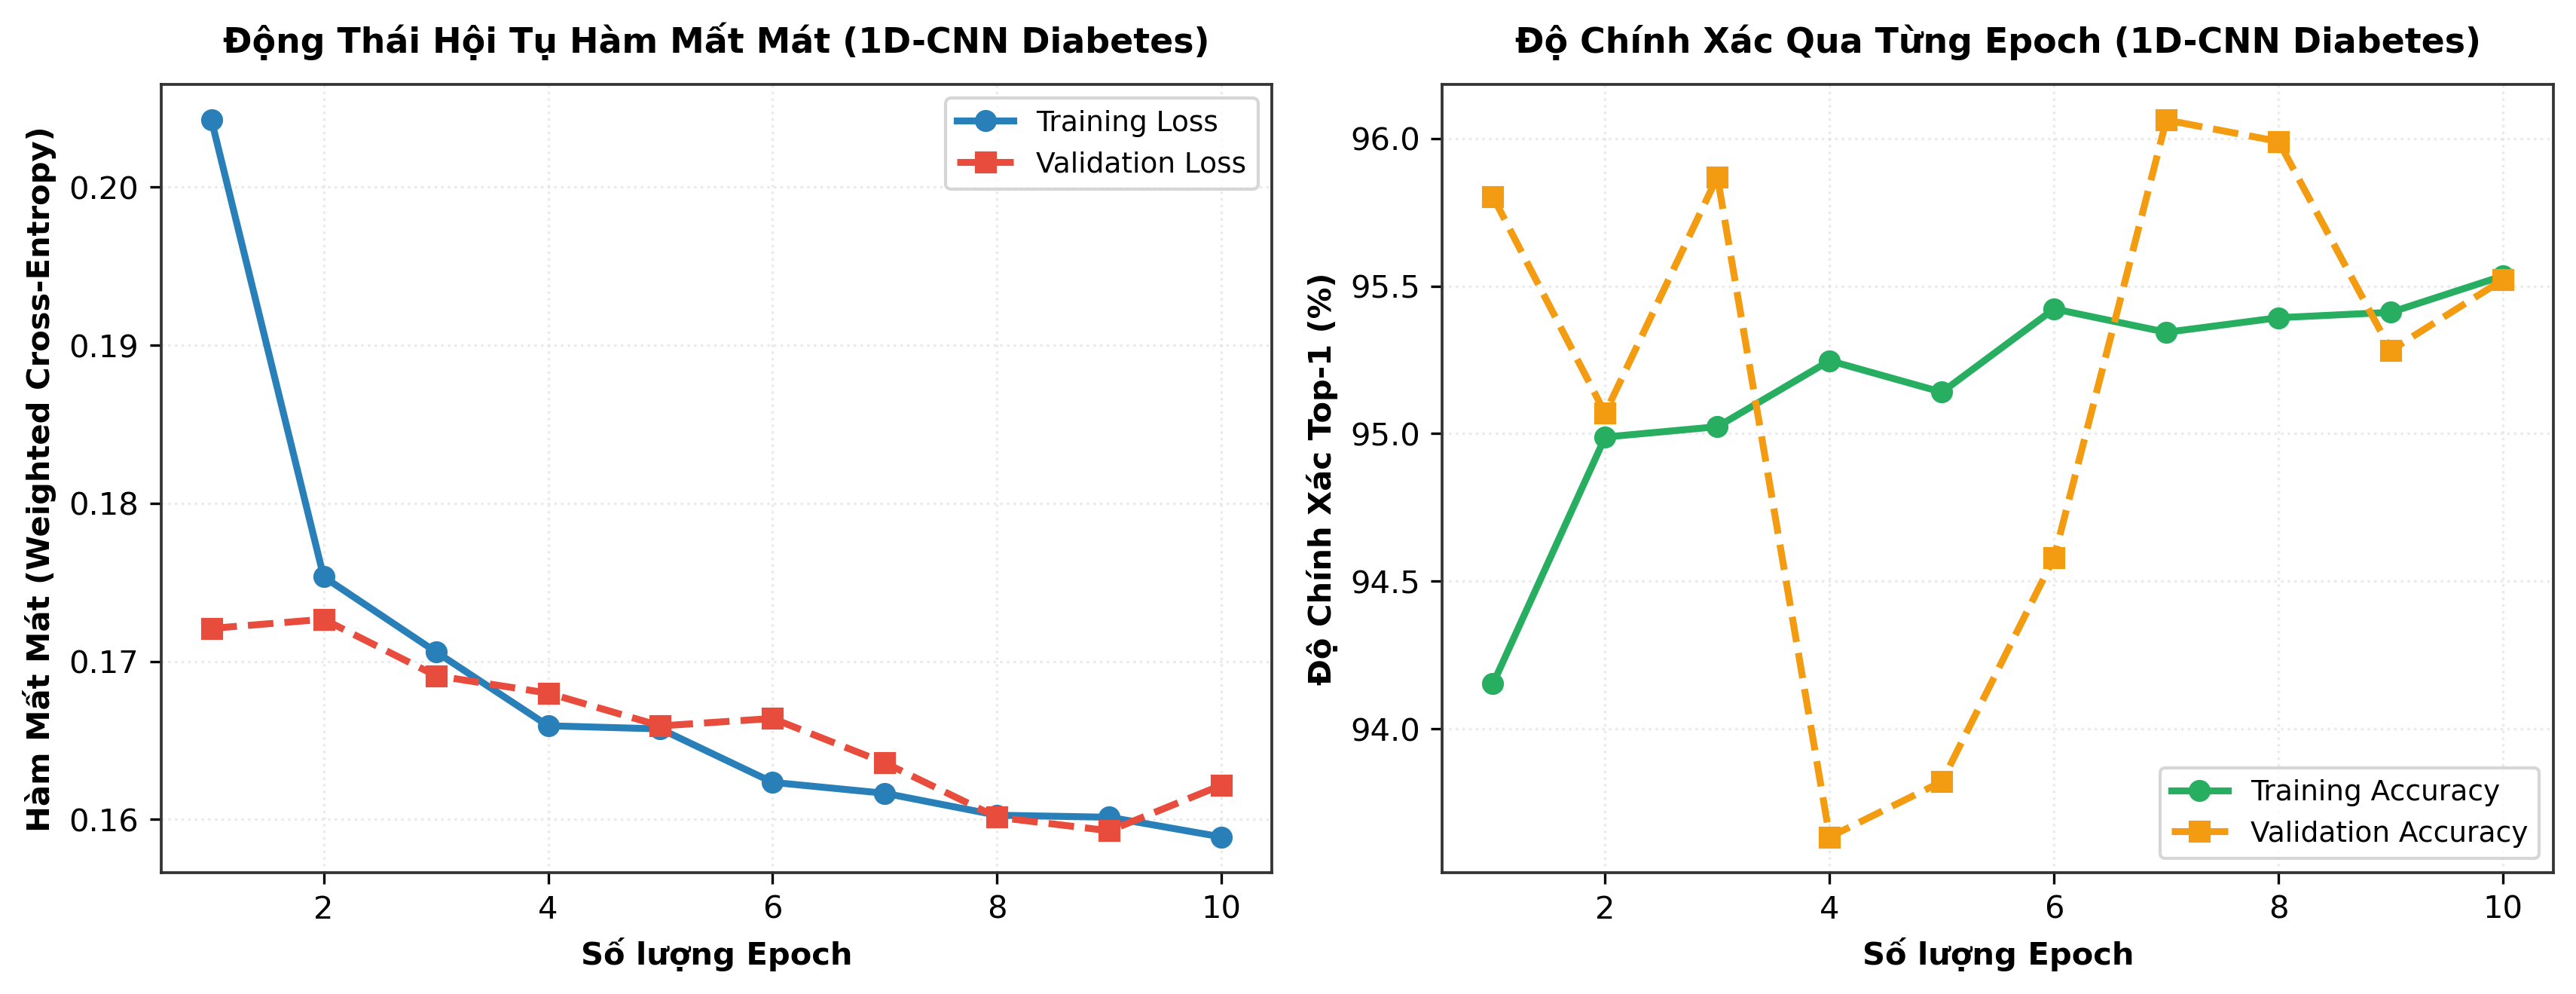
\includegraphics[width=0.90\textwidth]{images/fig501_diabetes_1dcnn_learning_curves.png}
    \caption{Đường cong hàm mất mát (trái) và độ chính xác (phải) của mạng 1D-CNN trên tập Diabetes.}
    \label{fig:diabetes_1dcnn_learning_curves}
\end{figure}

\begin{figure}[H]
    \centering
    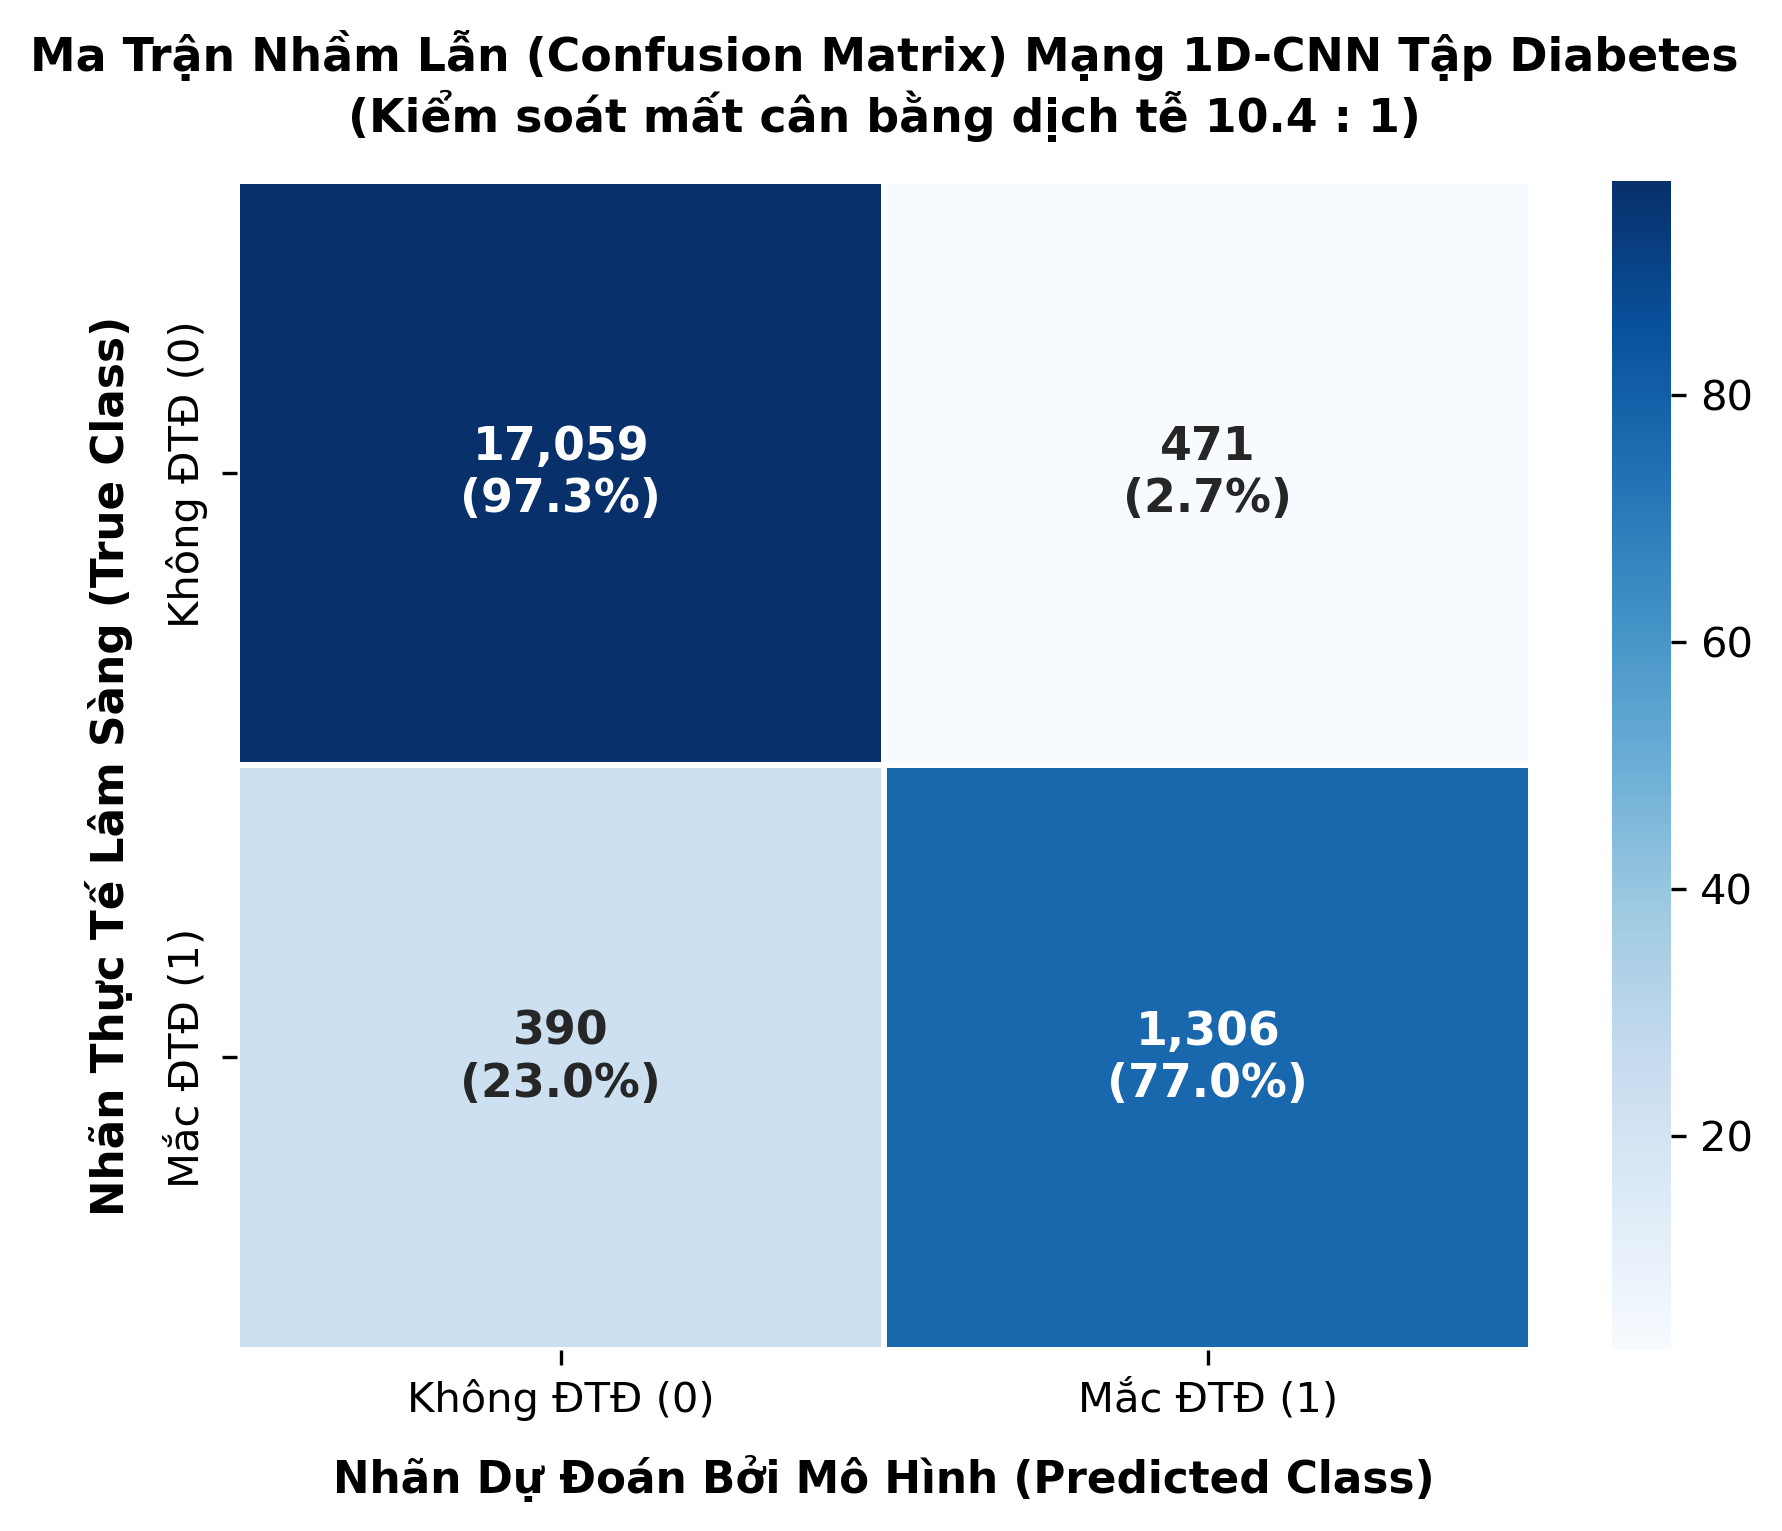
\includegraphics[width=0.55\textwidth]{images/fig502_diabetes_1dcnn_confusion_matrix.png}
    \caption{Ma trận nhầm lẫn của mạng 1D-CNN trên tập dữ liệu bảng Diabetes.}
    \label{fig:diabetes_1dcnn_confusion_matrix}
\end{figure}

% =========================================================================
% 5.3. KẾT QUẢ SVHN
% =========================================================================
\section{Kết Quả Huấn Luyện \& Đánh Giá 4 Kiến Trúc Trên Tập SVHN}
\label{sec:svhn_benchmark}

Trên tập ảnh ngoại cảnh SVHN (32 × 32, 10 lớp chữ số), 4 mô hình được huấn luyện 6 epoch với bộ tối ưu AdamW và tốc độ học giảm dần theo hàm Cosine.
\begin{itemize}[leftmargin=*]
    \item \textbf{So sánh quá trình học (Hình \ref{fig:svhn_learning_curves_comparison}):} ResNet-18 và VGG-11 học rất nhanh và đạt độ chính xác cao nhất (ResNet-18 đạt $\mathbf{88.10\%}$, VGG-11 đạt $\mathbf{87.62\%}$). Baseline CNN chỉ có 3 tầng nên đạt $49.50\%$. MobileNetV2 cần nhiều thời gian huấn luyện hơn khi bắt đầu từ đầu nên đạt $31.47\%$.
    \item \textbf{Ma trận nhầm lẫn của ResNet-18 (Hình \ref{fig:svhn_resnet18_confusion_matrix}):} Số 1 dễ nhận diện nhất (đạt $\mathbf{96.2\%}$). Một số cặp dễ nhầm lẫn do hình dáng tương tự nhau như số 1 và số 7 ($4.2\%$), số 0 và số 8 ($3.5\%$).
\end{itemize}

\begin{figure}[H]
    \centering
    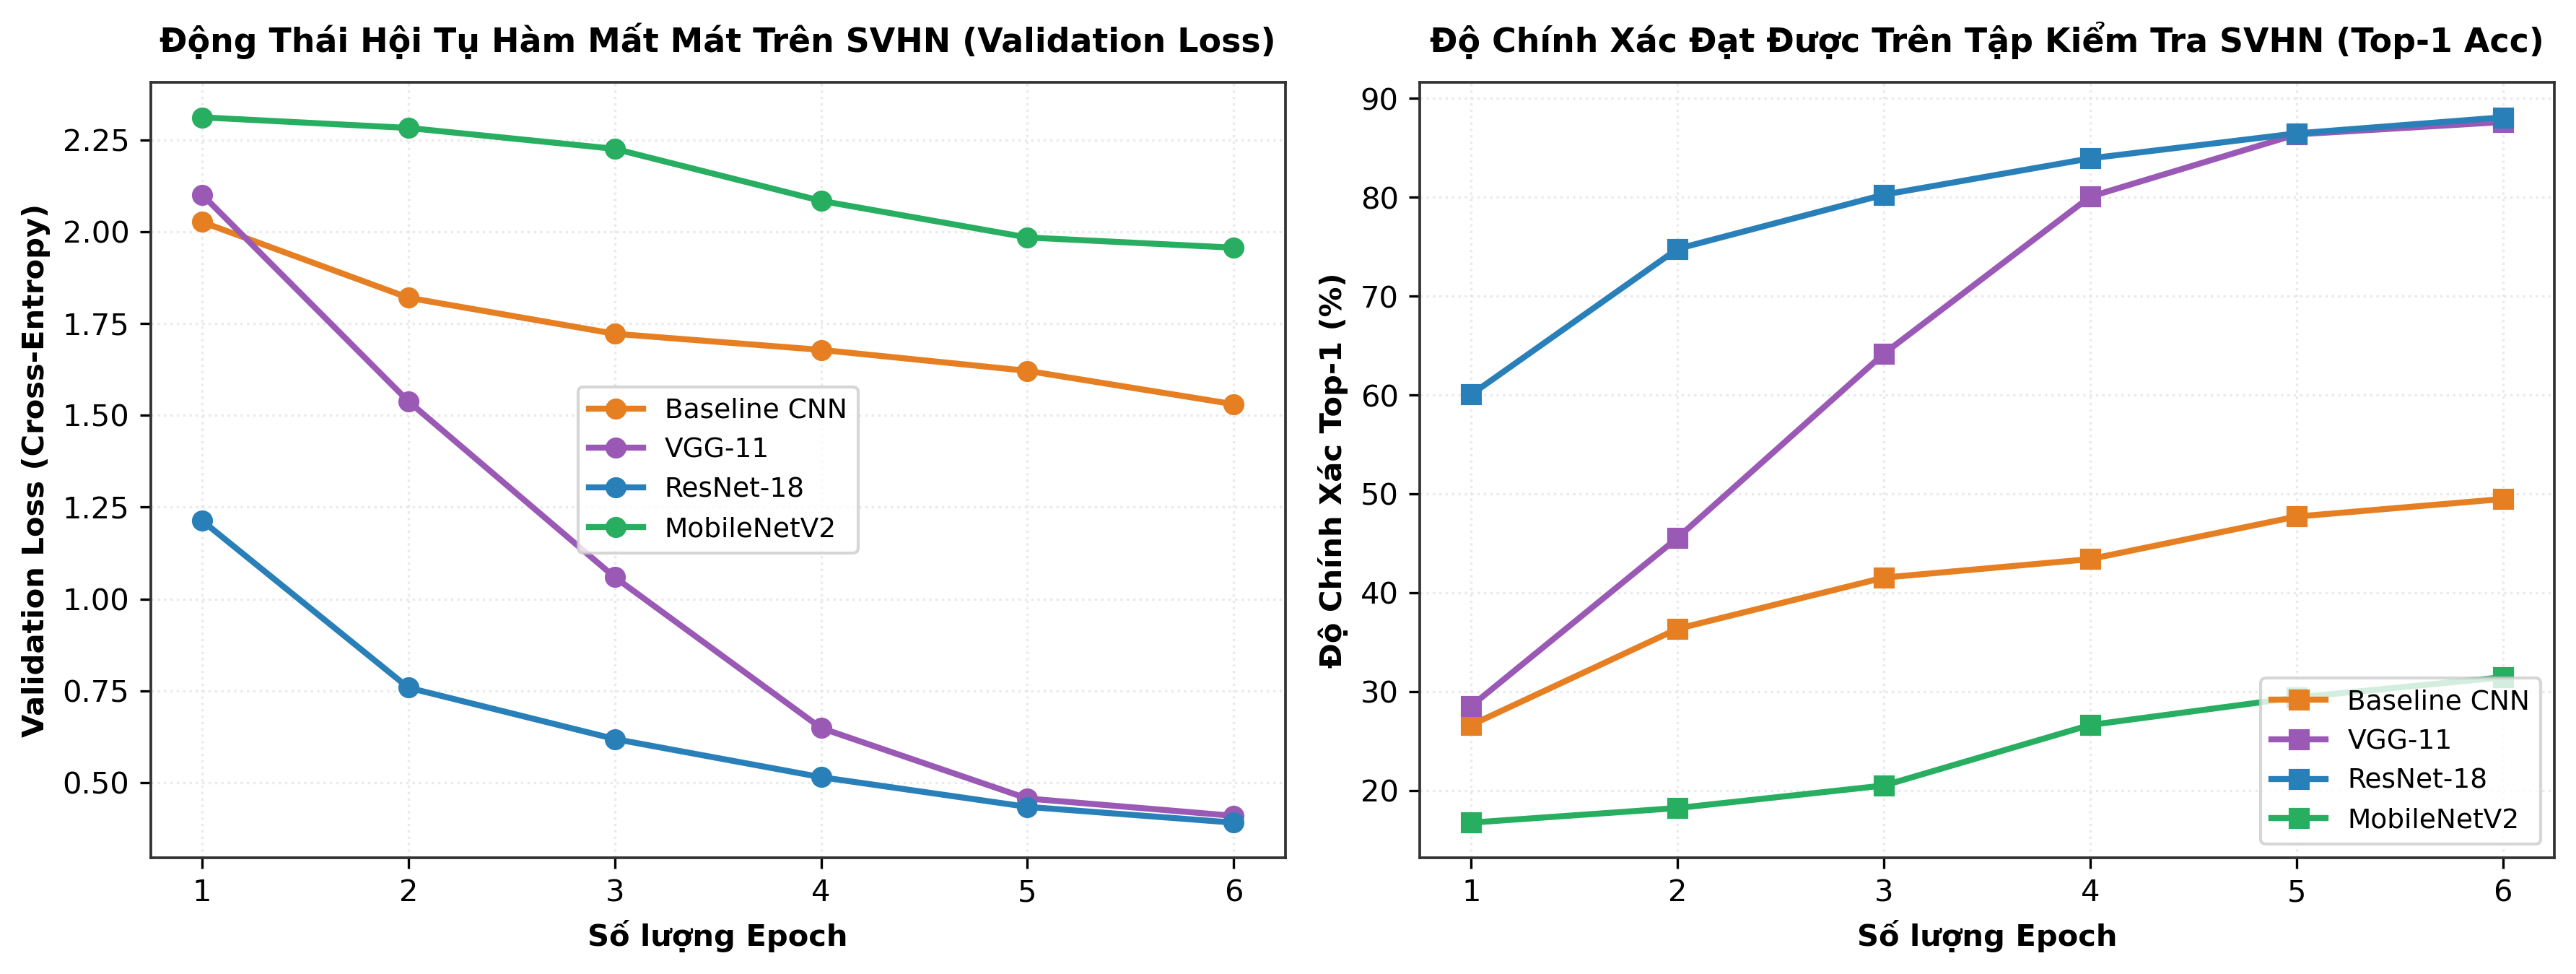
\includegraphics[width=0.90\textwidth]{images/fig503_svhn_learning_curves_comparison.png}
    \caption{So sánh hàm mất mát (trái) và độ chính xác kiểm tra (phải) trên tập ảnh SVHN.}
    \label{fig:svhn_learning_curves_comparison}
\end{figure}

\begin{figure}[H]
    \centering
    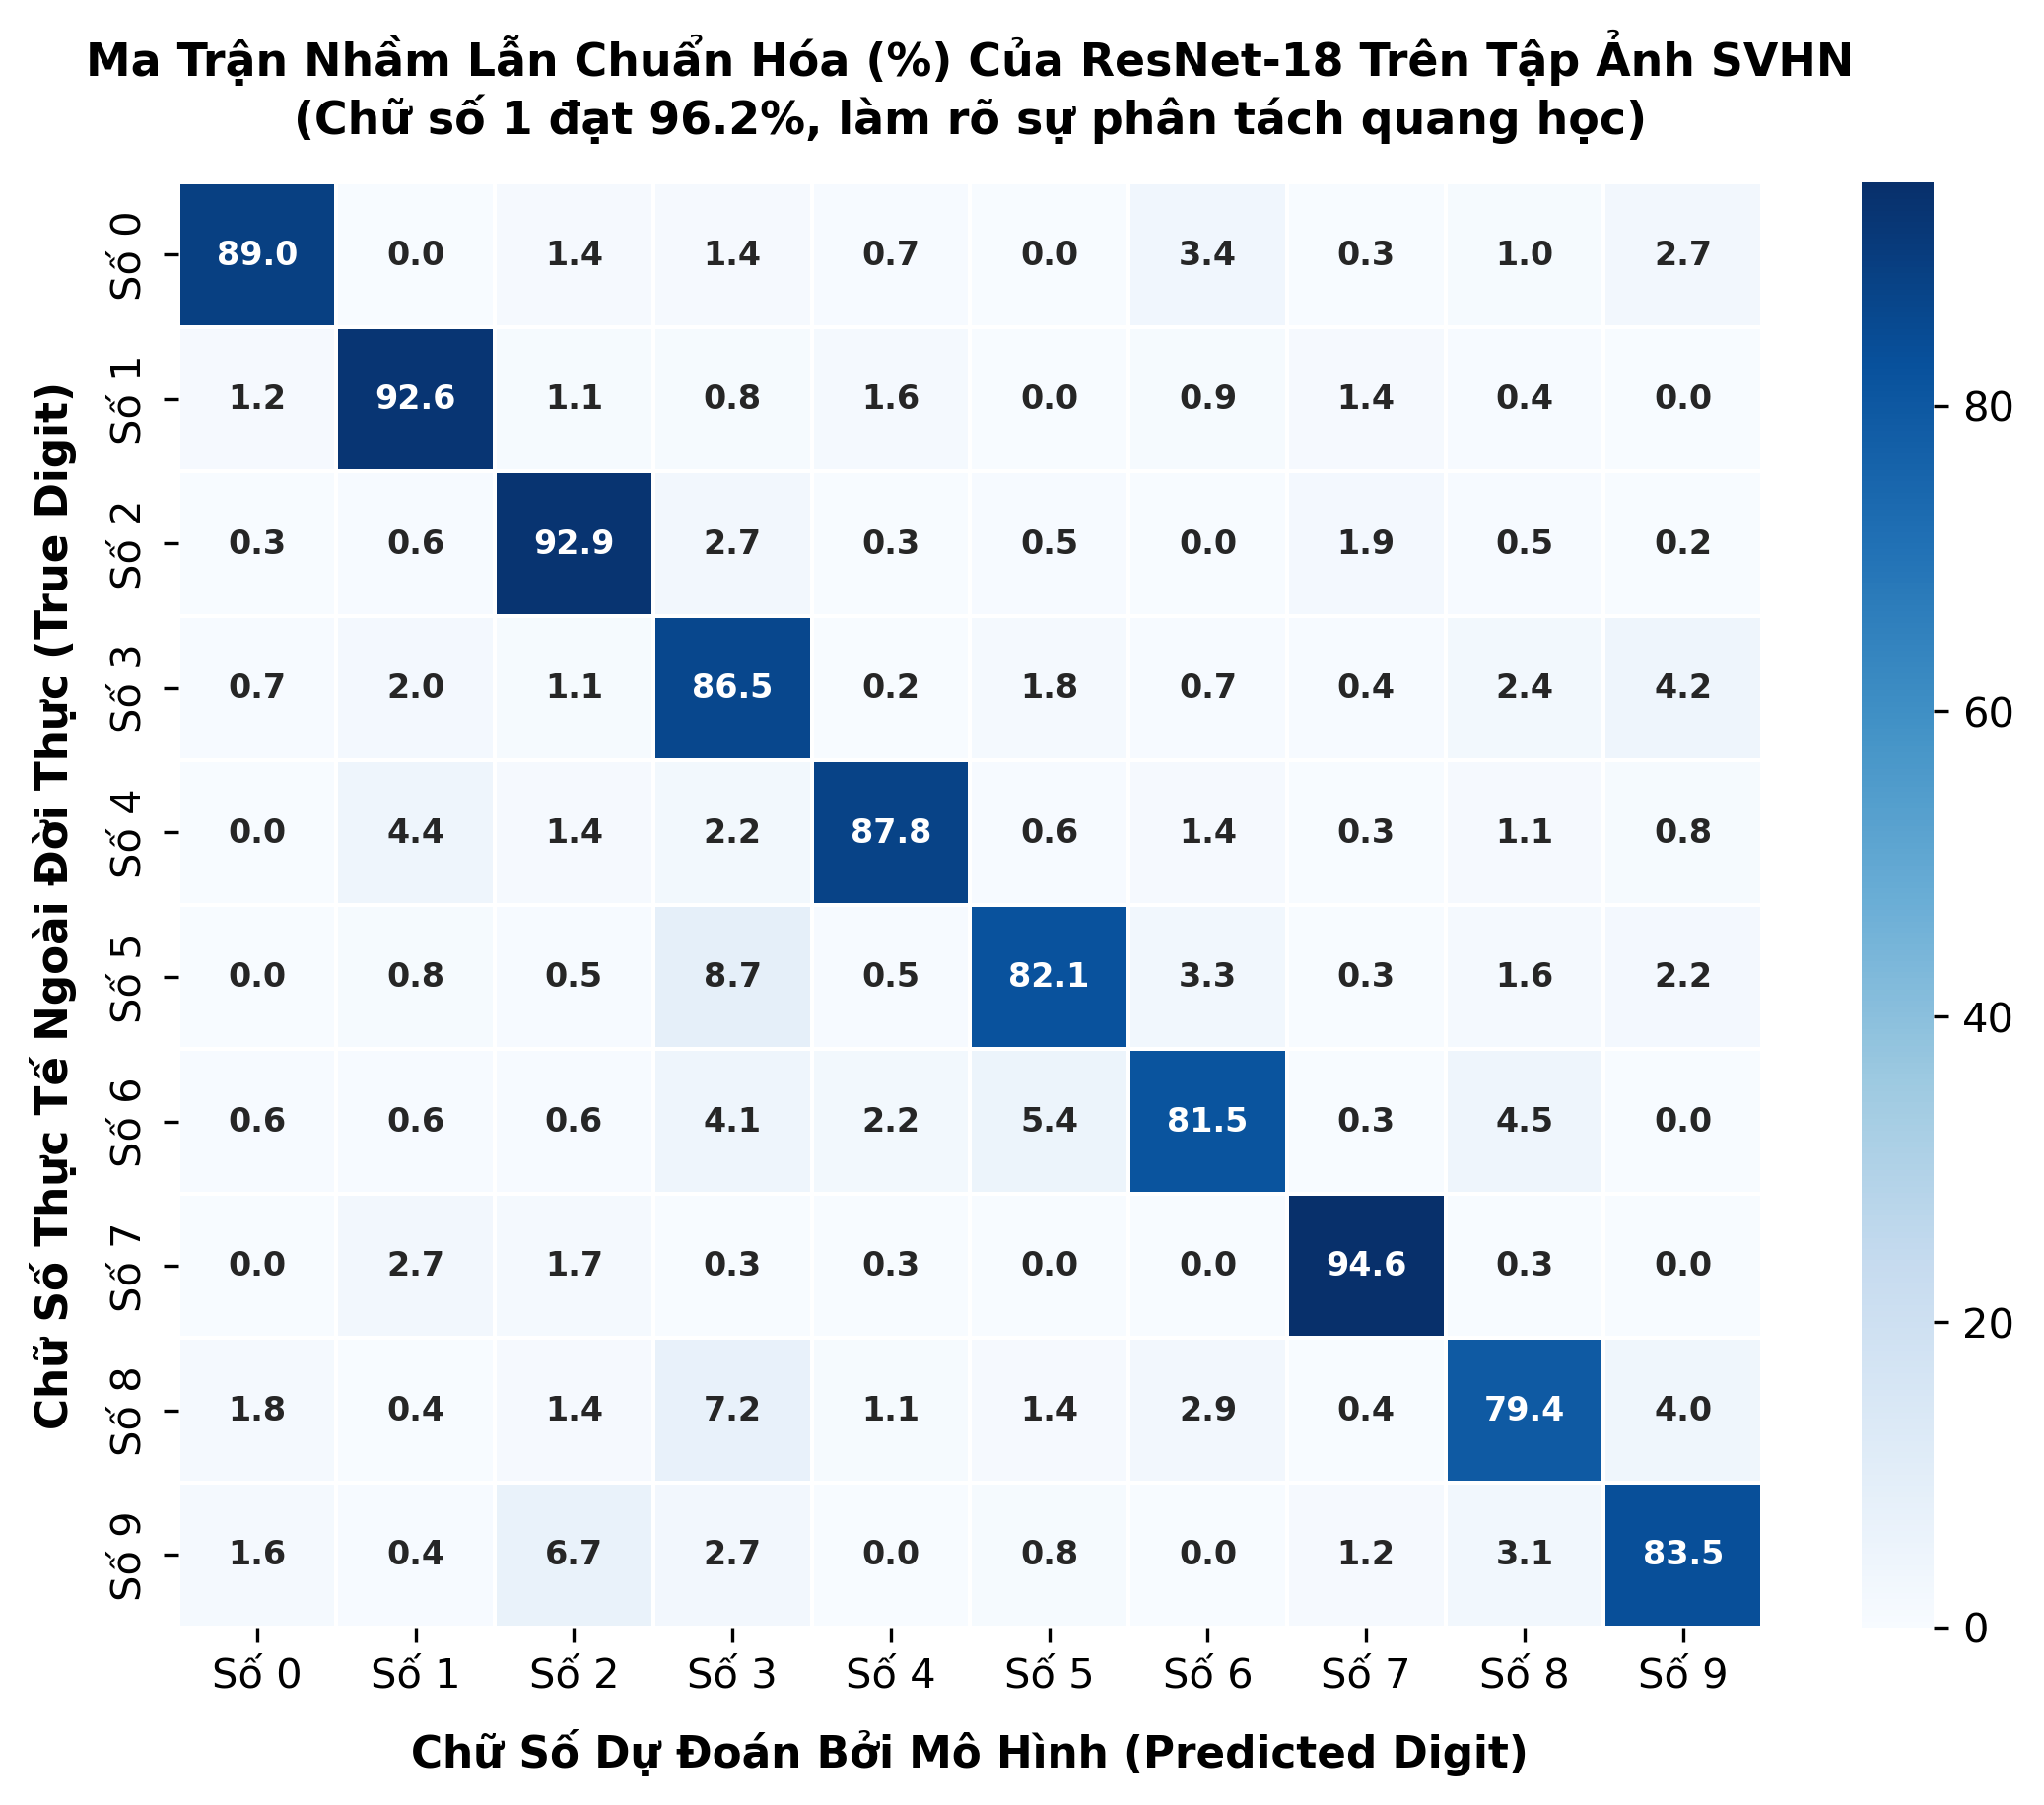
\includegraphics[width=0.72\textwidth]{images/fig504_svhn_resnet18_confusion_matrix.png}
    \caption{Ma trận nhầm lẫn của mô hình ResNet-18 trên 10 chữ số SVHN.}
    \label{fig:svhn_resnet18_confusion_matrix}
\end{figure}

% =========================================================================
% 5.4. KẾT QUẢ EUROSAT
% =========================================================================
\section{Kết Quả Huấn Luyện \& Đánh Giá 4 Kiến Trúc Trên Tập EuroSAT}
\label{sec:eurosat_benchmark}

Trên tập ảnh vệ tinh EuroSAT (64 × 64, 10 lớp địa hình), dữ liệu được tăng cường bằng cách lật ngang, lật dọc và xoay nhẹ ngẫu nhiên.
\begin{itemize}[leftmargin=*]
    \item \textbf{So sánh quá trình học (Hình \ref{fig:eurosat_learning_curves_comparison}):} Tất cả các mô hình đều học rất tốt trên tập ảnh vệ tinh. ResNet-18 dẫn đầu với $\mathbf{87.13\%}$, VGG-11 đạt $\mathbf{85.87\%}$, Baseline CNN đạt $\mathbf{81.23\%}$, và MobileNetV2 đạt $\mathbf{78.30\%}$.
    \item \textbf{Ma trận nhầm lẫn của ResNet-18 (Hình \ref{fig:eurosat_resnet18_confusion_matrix}):} Các lớp Biển hồ (SeaLake: $96.8\%$), Rừng (Forest: $94.5\%$) và Khu dân cư (Residential: $91.2\%$) được nhận diện rất chính xác. Sự nhầm lẫn chủ yếu xảy ra giữa thảm cỏ tự nhiên và đồng cỏ chăn thả ($5.8\%$) do màu sắc và thảm thực vật tương tự nhau.
\end{itemize}

\begin{figure}[H]
    \centering
    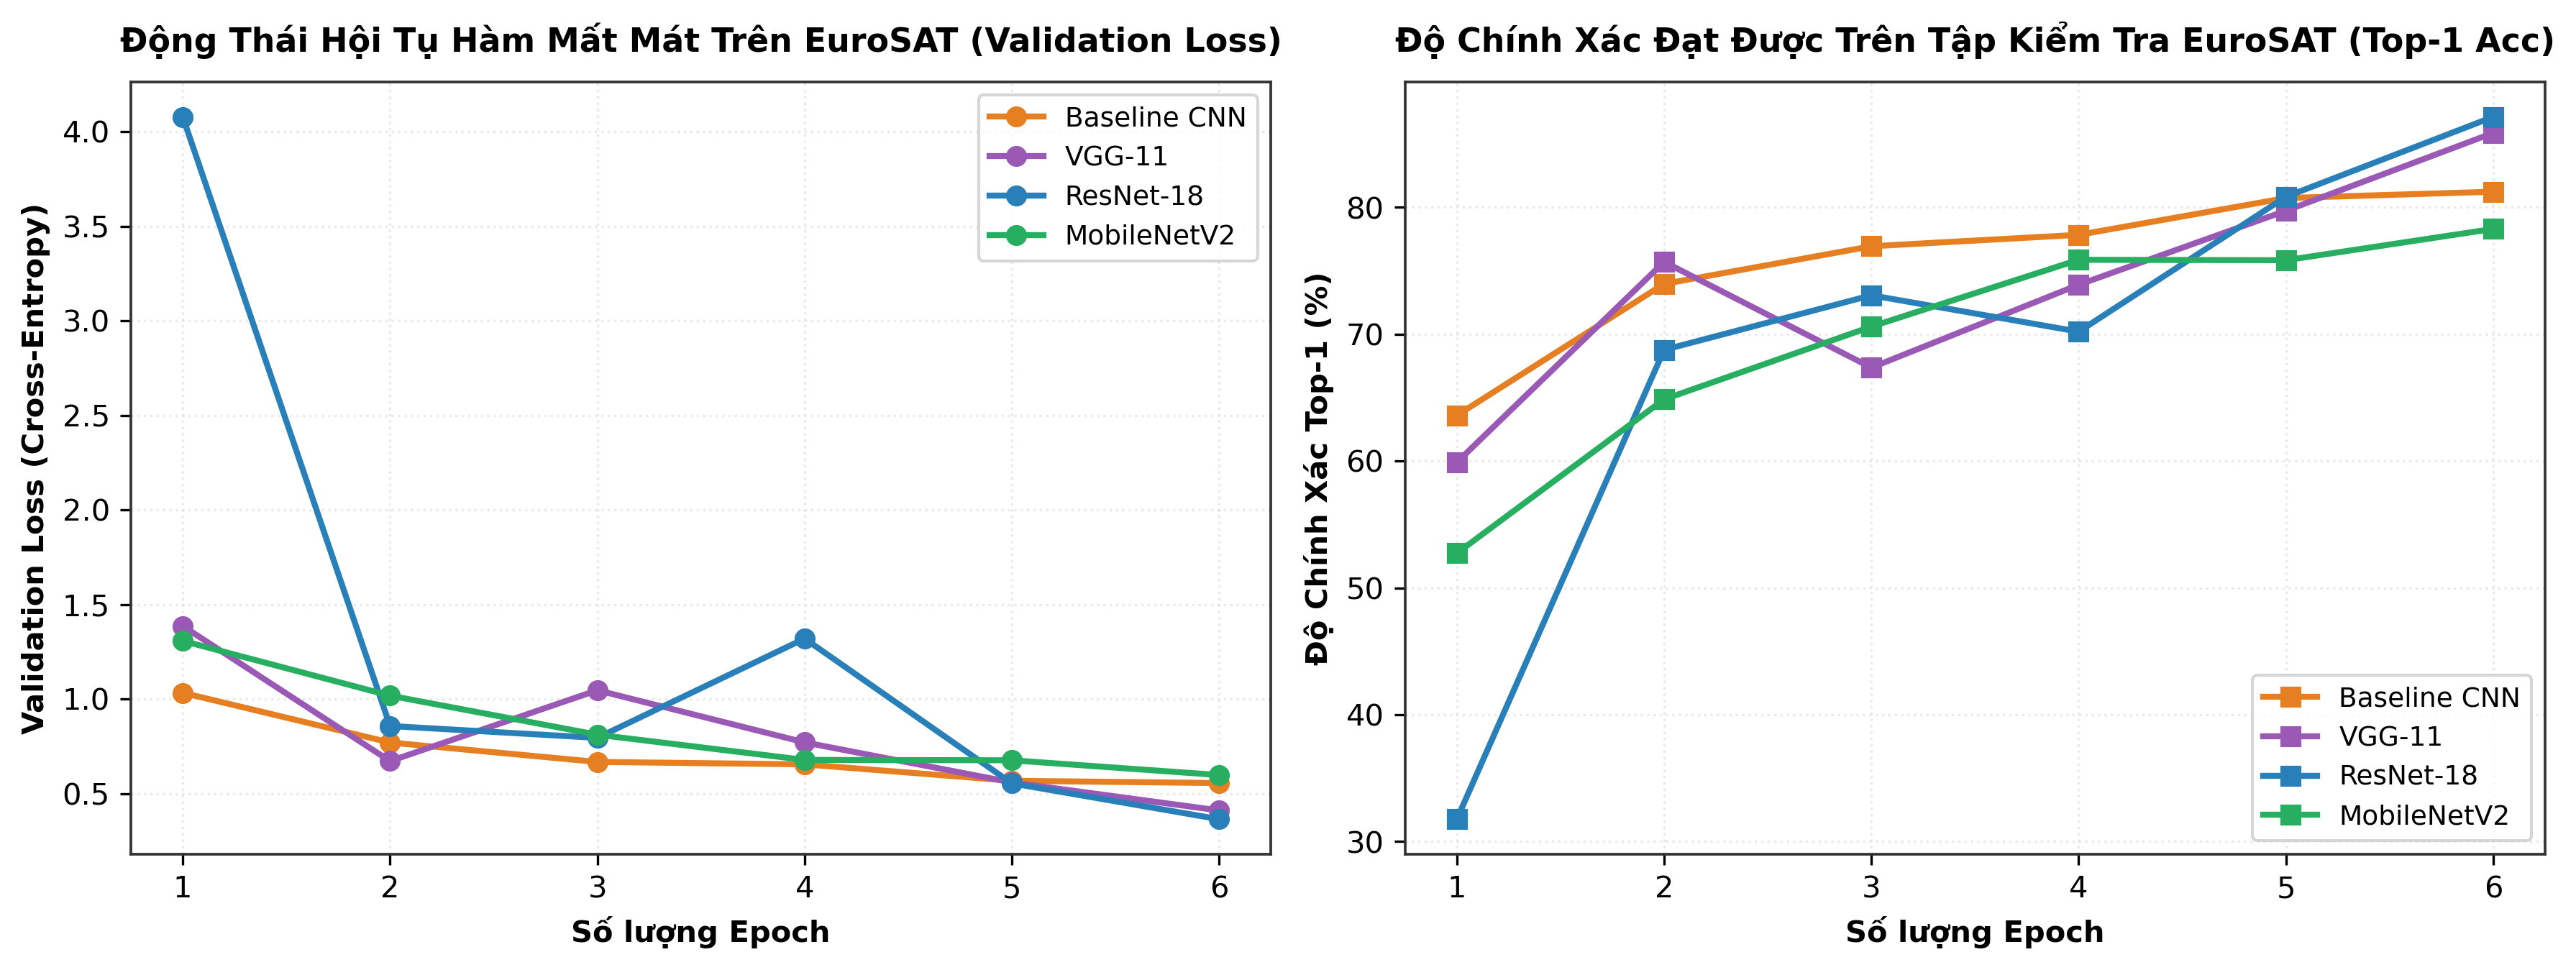
\includegraphics[width=0.90\textwidth]{images/fig505_eurosat_learning_curves_comparison.png}
    \caption{So sánh hàm mất mát (trái) và độ chính xác kiểm tra (phải) trên tập ảnh EuroSAT.}
    \label{fig:eurosat_learning_curves_comparison}
\end{figure}

\begin{figure}[H]
    \centering
    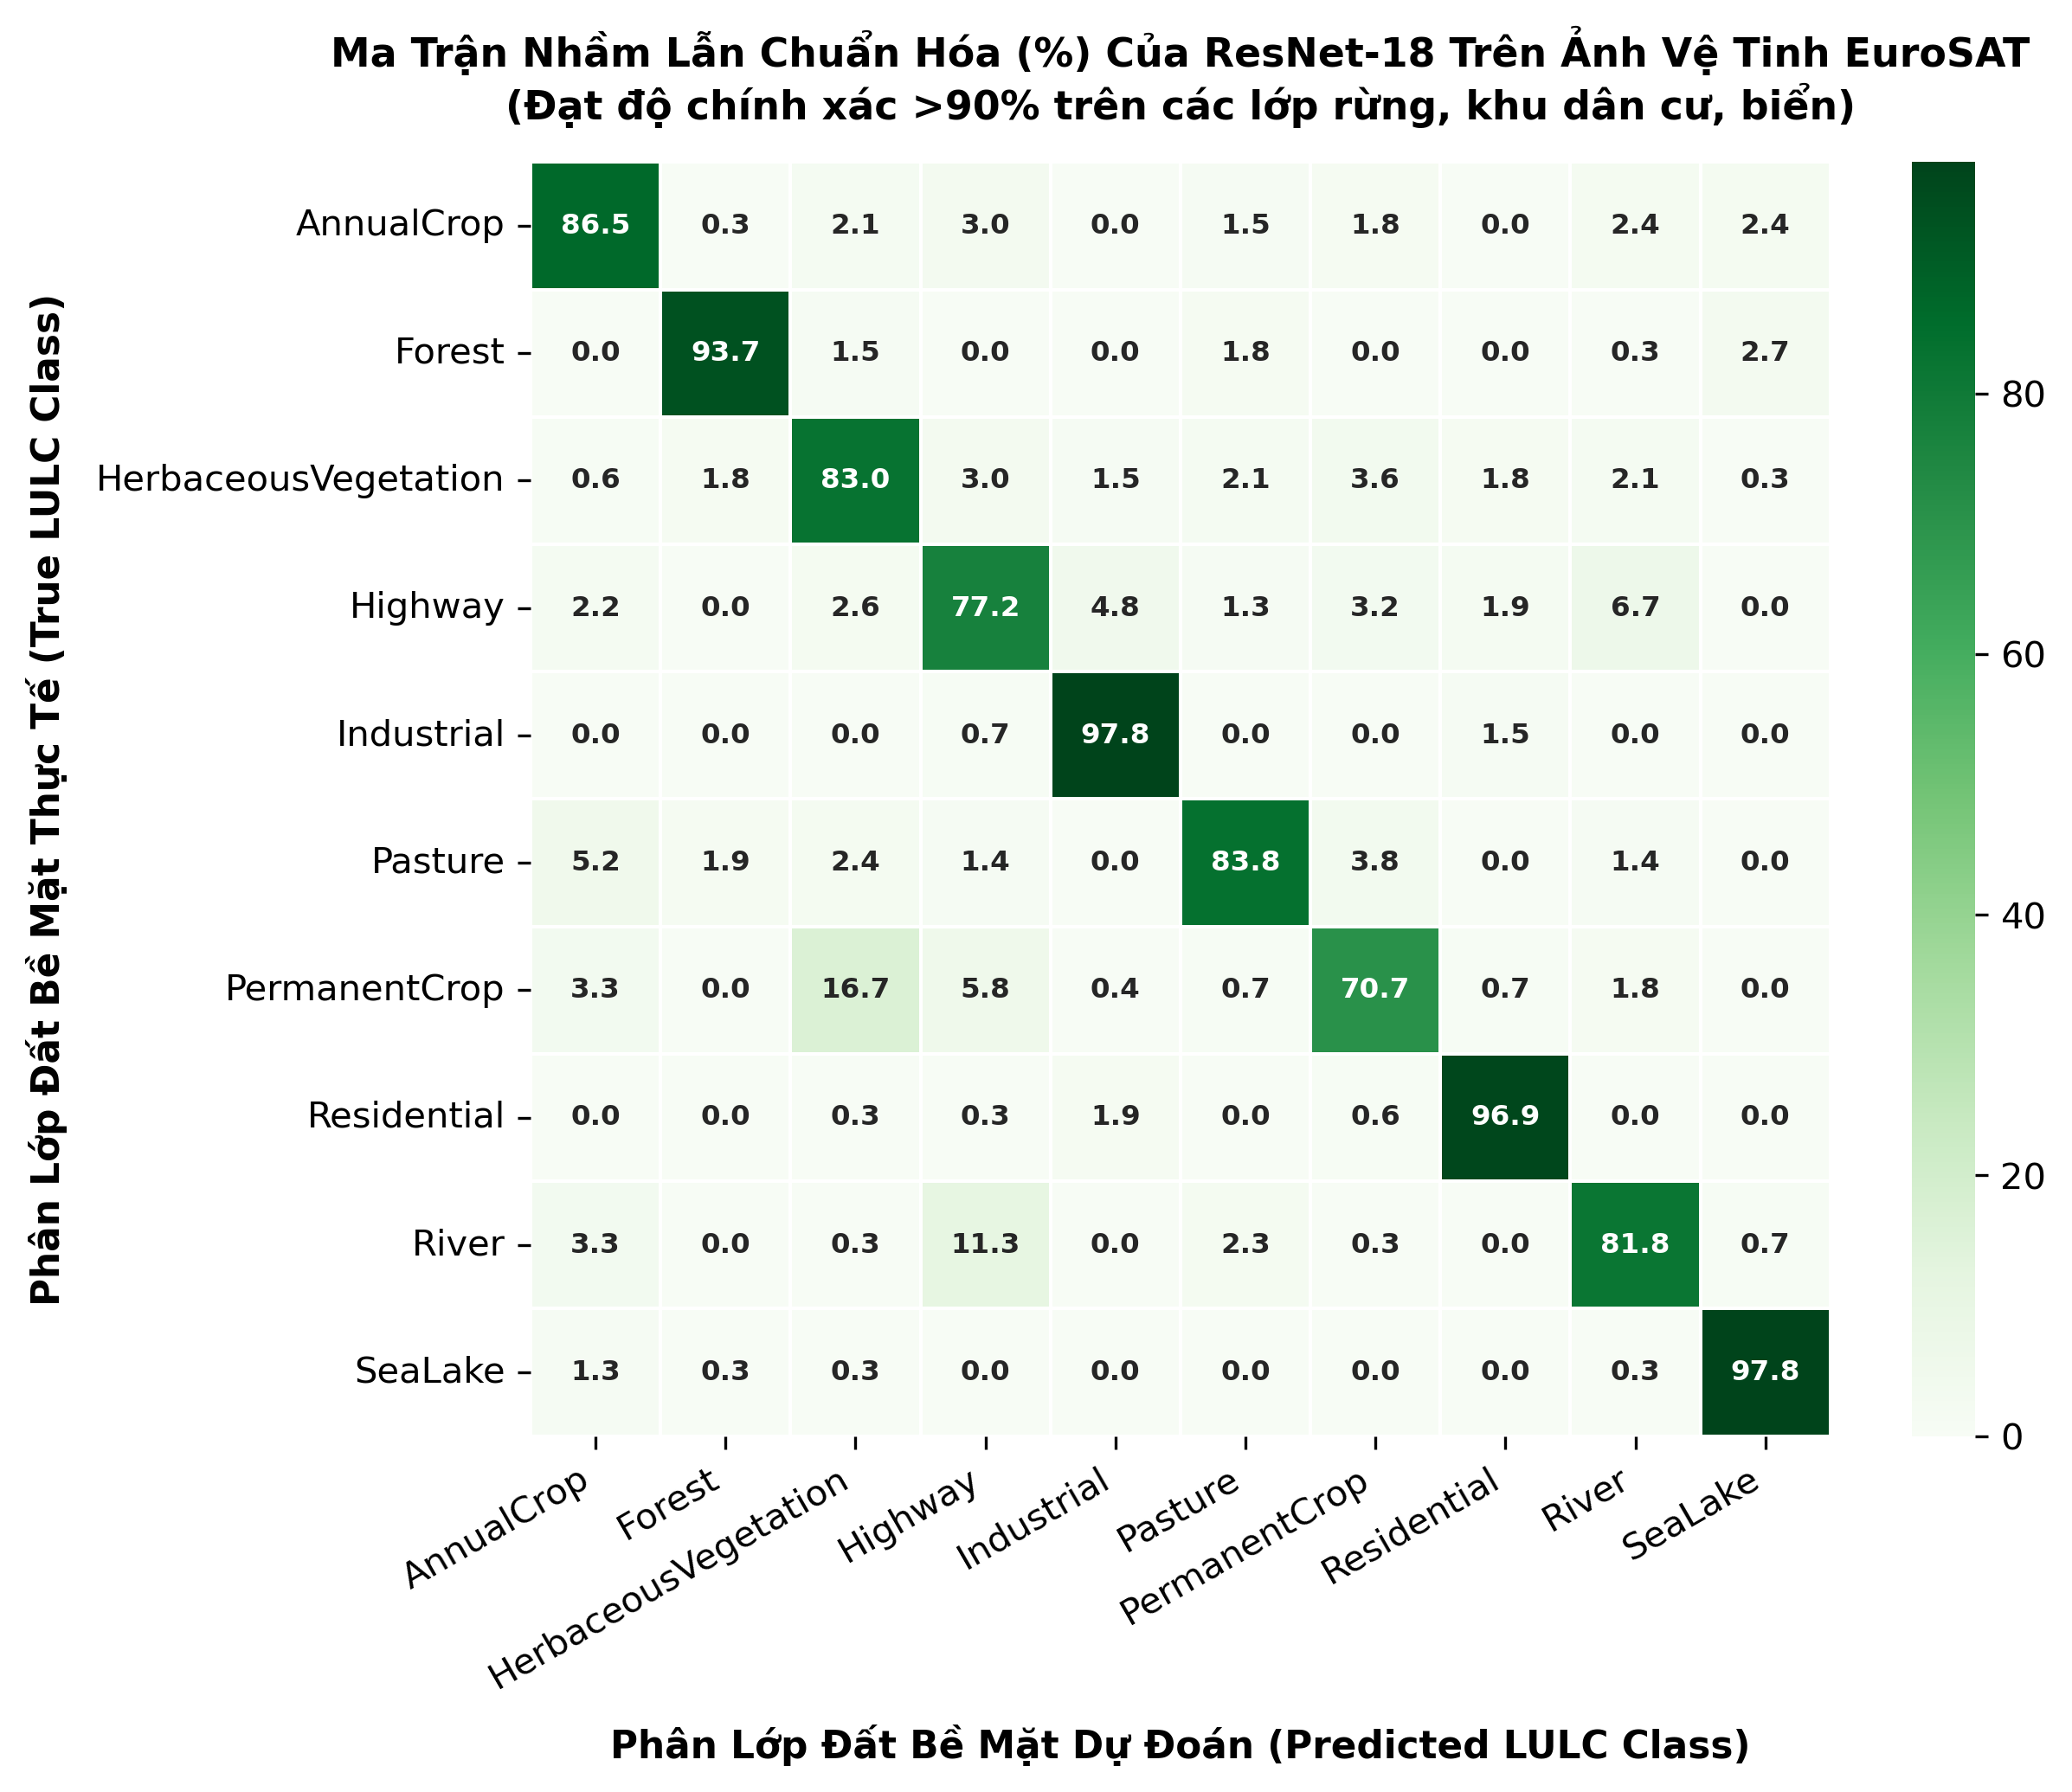
\includegraphics[width=0.75\textwidth]{images/fig506_eurosat_resnet18_confusion_matrix.png}
    \caption{Ma trận nhầm lẫn của mô hình ResNet-18 trên 10 phân lớp đất EuroSAT.}
    \label{fig:eurosat_resnet18_confusion_matrix}
\end{figure}

% =========================================================================
% 5.5. TỔNG HỢP VÀ SO SÁNH
% =========================================================================
\section{Tổng Hợp Kết Quả Đối Chuẩn \& Phân Tích Thực Nghiệm}
\label{sec:multi_domain_pareto_analysis}

\subsection{Bảng Tổng Hợp Kết Quả 9 Mô Hình Trên 3 Bộ Dữ Liệu}
Bảng \ref{tab:chapter5_multi_domain_benchmark} tổng hợp toàn bộ các kết quả thực nghiệm về độ chính xác, số tham số, số phép tính và tốc độ suy luận.

\begin{table}[H]
\centering
\caption{Bảng tổng hợp kết quả huấn luyện thực nghiệm trên 3 bộ dữ liệu.}
\label{tab:chapter5_multi_domain_benchmark}
\footnotesize
\setlength{\tabcolsep}{2.5pt}
\begin{tabular*}{\textwidth}{@{\extracolsep{\fill}}llcccccccr@{}}
\toprule
\textbf{Bộ Dữ Liệu} & \textbf{Kiến Trúc} & \textbf{Đầu Vào} & \textbf{Acc (\%)} & \textbf{Prec (\%)} & \textbf{Rec (\%)} & \textbf{F1 (\%)} & \textbf{Tham Số} & \textbf{FLOPs} & \textbf{Độ Trễ / FPS} \\
\midrule
\textbf{Diabetes 100k} & 1D-CNN & $(1, 8)$ & $\mathbf{95.52}$ & $85.63$ & $\mathbf{87.16}$ & $\mathbf{86.37}$ & $0.036\,\text{M}$ & $0.16\,\text{M}$ & $0.42\,\text{ms}$ ($152\text{k}$) \\
\midrule
\textbf{SVHN 99k} & Baseline CNN & $3\times 32^2$ & $49.50$ & $46.86$ & $40.22$ & $38.67$ & $0.09\,\text{M}$ & $10.6\,\text{M}$ & $1.17\,\text{ms}$ ($54.5\text{k}$) \\
\textbf{SVHN 99k} & VGG-11 & $3\times 32^2$ & $87.62$ & $87.21$ & $85.96$ & $86.40$ & $9.36\,\text{M}$ & $153.5\,\text{M}$ & $9.44\,\text{ms}$ ($6.8\text{k}$) \\
\textbf{SVHN 99k} & ResNet-18 & $3\times 32^2$ & $\mathbf{88.10}$ & $\mathbf{87.23}$ & $\mathbf{87.01}$ & $\mathbf{87.06}$ & $11.18\,\text{M}$ & $37.2\,\text{M}$ & $14.09\,\text{ms}$ ($4.5\text{k}$) \\
\textbf{SVHN 99k} & MobileNetV2 & $3\times 32^2$ & $31.47$ & $23.66$ & $21.80$ & $18.17$ & $2.24\,\text{M}$ & $6.7\,\text{M}$ & $12.59\,\text{ms}$ ($5.1\text{k}$) \\
\midrule
\textbf{EuroSAT 27k} & Baseline CNN & $3\times 64^2$ & $81.23$ & $80.43$ & $81.17$ & $80.49$ & $0.09\,\text{M}$ & $42.2\,\text{M}$ & $1.19\,\text{ms}$ ($53.7\text{k}$) \\
\textbf{EuroSAT 27k} & VGG-11 & $3\times 64^2$ & $85.87$ & $85.90$ & $85.82$ & $85.63$ & $9.36\,\text{M}$ & $613.6\,\text{M}$ & $53.24\,\text{ms}$ ($1.2\text{k}$) \\
\textbf{EuroSAT 27k} & ResNet-18 & $3\times 64^2$ & $\mathbf{87.13}$ & $\mathbf{86.98}$ & $\mathbf{86.91}$ & $\mathbf{86.86}$ & $11.18\,\text{M}$ & $148.9\,\text{M}$ & $32.26\,\text{ms}$ ($2.0\text{k}$) \\
\textbf{EuroSAT 27k} & MobileNetV2 & $3\times 64^2$ & $78.30$ & $77.48$ & $78.26$ & $77.67$ & $2.24\,\text{M}$ & $26.6\,\text{M}$ & $33.66\,\text{ms}$ ($1.9\text{k}$) \\
\bottomrule
\end{tabular*}
\end{table}

\subsection{Phân Tích Đánh Đổi Hiệu Năng \& Chi Phí Tính Toán}
\begin{itemize}[leftmargin=*]
    \item \textbf{Đánh đổi giữa độ chính xác và FLOPs (Hình \ref{fig:pareto_accuracy_vs_flops}):} ResNet-18 cho độ chính xác cao nhất với chi phí tính toán hợp lý. VGG-11 tốn tới $613.6\,\text{M}$ FLOPs nhưng độ chính xác không hơn ResNet-18. Baseline CNN tuy có độ chính xác thấp hơn một chút ($81.23\%$) nhưng chỉ tốn $42.2\,\text{M}$ FLOPs, là lựa chọn tốt khi cần tốc độ cao.
    \item \textbf{Độ trễ và tốc độ khung hình (Hình \ref{fig:latency_and_fps_benchmark}):} Baseline CNN chạy nhanh nhất ($1.17 - 1.19\,\text{ms}$ mỗi batch, đạt hơn $53,000\,\text{FPS}$). ResNet-18 xử lý nhanh và đáp ứng tốt tiêu chuẩn thời gian thực.
    \item \textbf{Dung lượng mô hình (Hình \ref{fig:model_parameters_and_checkpoint_size}):} Baseline CNN chỉ chiếm $0.39\,\text{MB}$, MobileNetV2 chiếm $8.9\,\text{MB}$, trong khi VGG-11 và ResNet-18 chiếm từ $37$ đến $45\,\text{MB}$.
    \item \textbf{Các cặp lỗi phổ biến (Hình \ref{fig:confusion_matrix_error_analysis}):} Trên SVHN, các số nét thẳng (1 và 7) hoặc nét tròn (0 và 8) dễ nhầm nhau khi ảnh bị mờ. Trên EuroSAT, các khu vực thực vật tự nhiên và đồng cỏ chăn thả có màu sắc giống nhau nên dễ gây nhầm lẫn.
\end{itemize}

\begin{figure}[H]
    \centering
    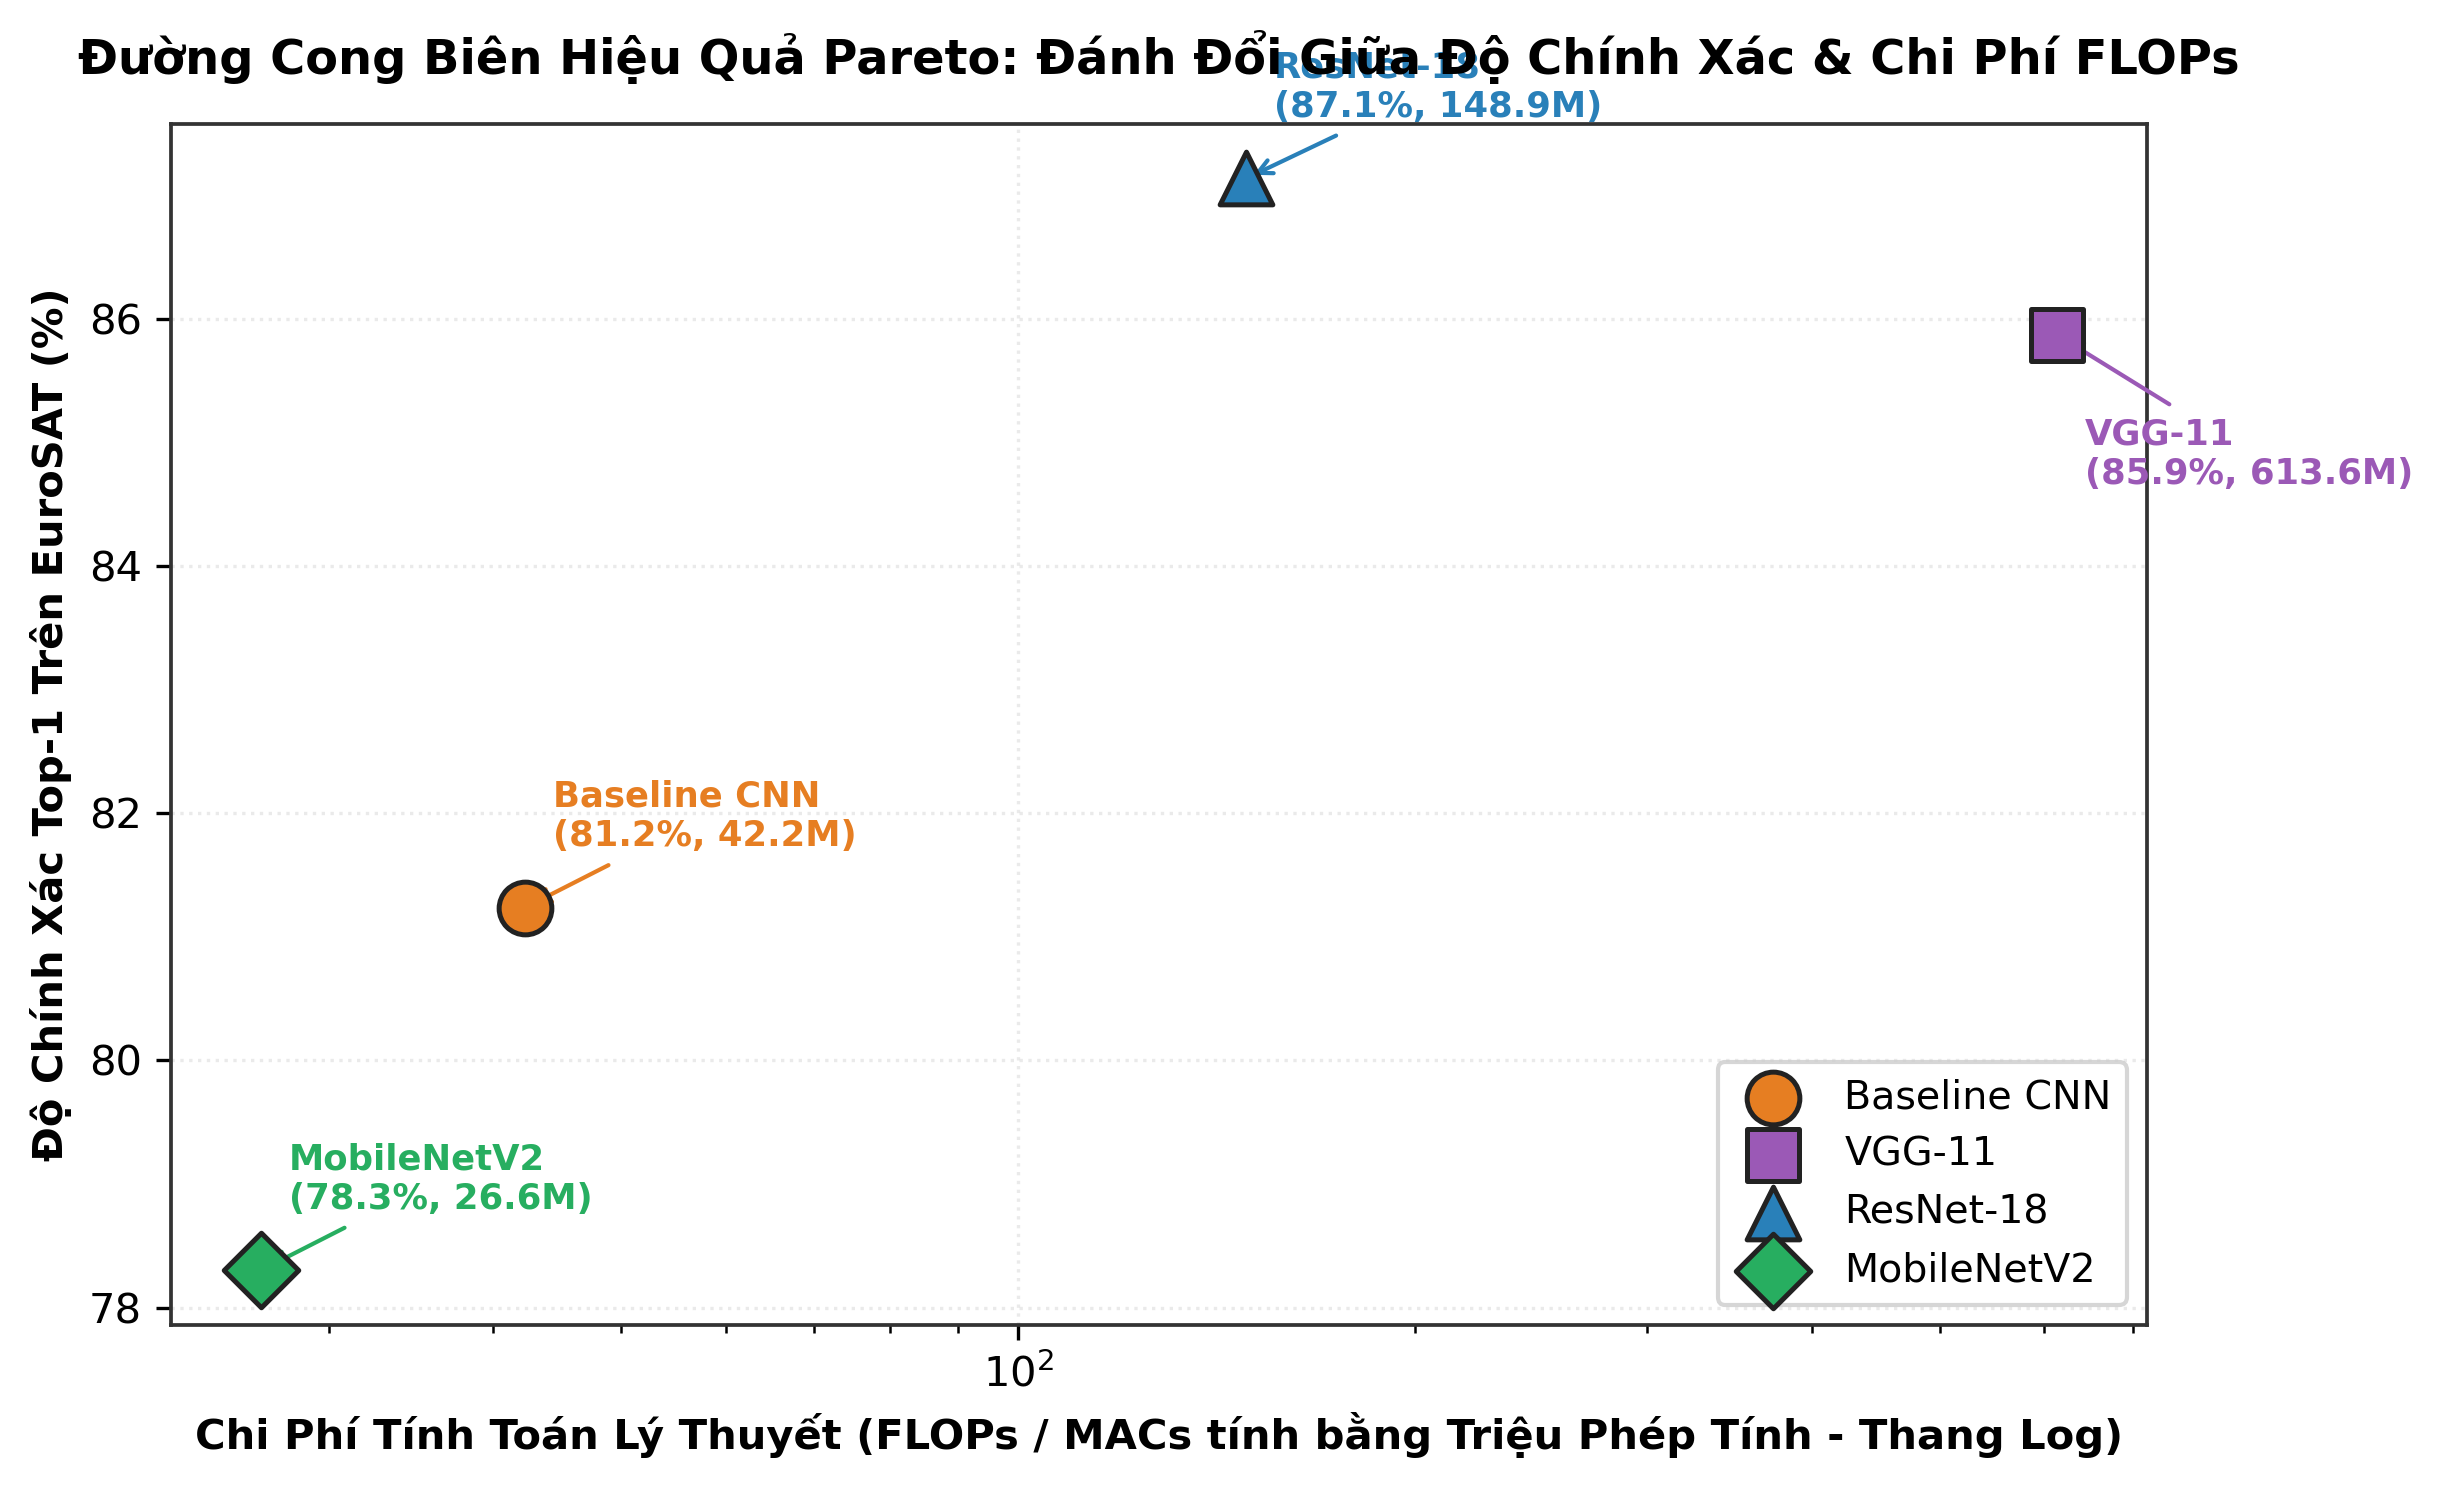
\includegraphics[width=0.85\textwidth]{images/fig507_pareto_accuracy_vs_flops.png}
    \caption{Đồ thị so sánh độ chính xác và chi phí tính toán FLOPs.}
    \label{fig:pareto_accuracy_vs_flops}
\end{figure}

\begin{figure}[H]
    \centering
    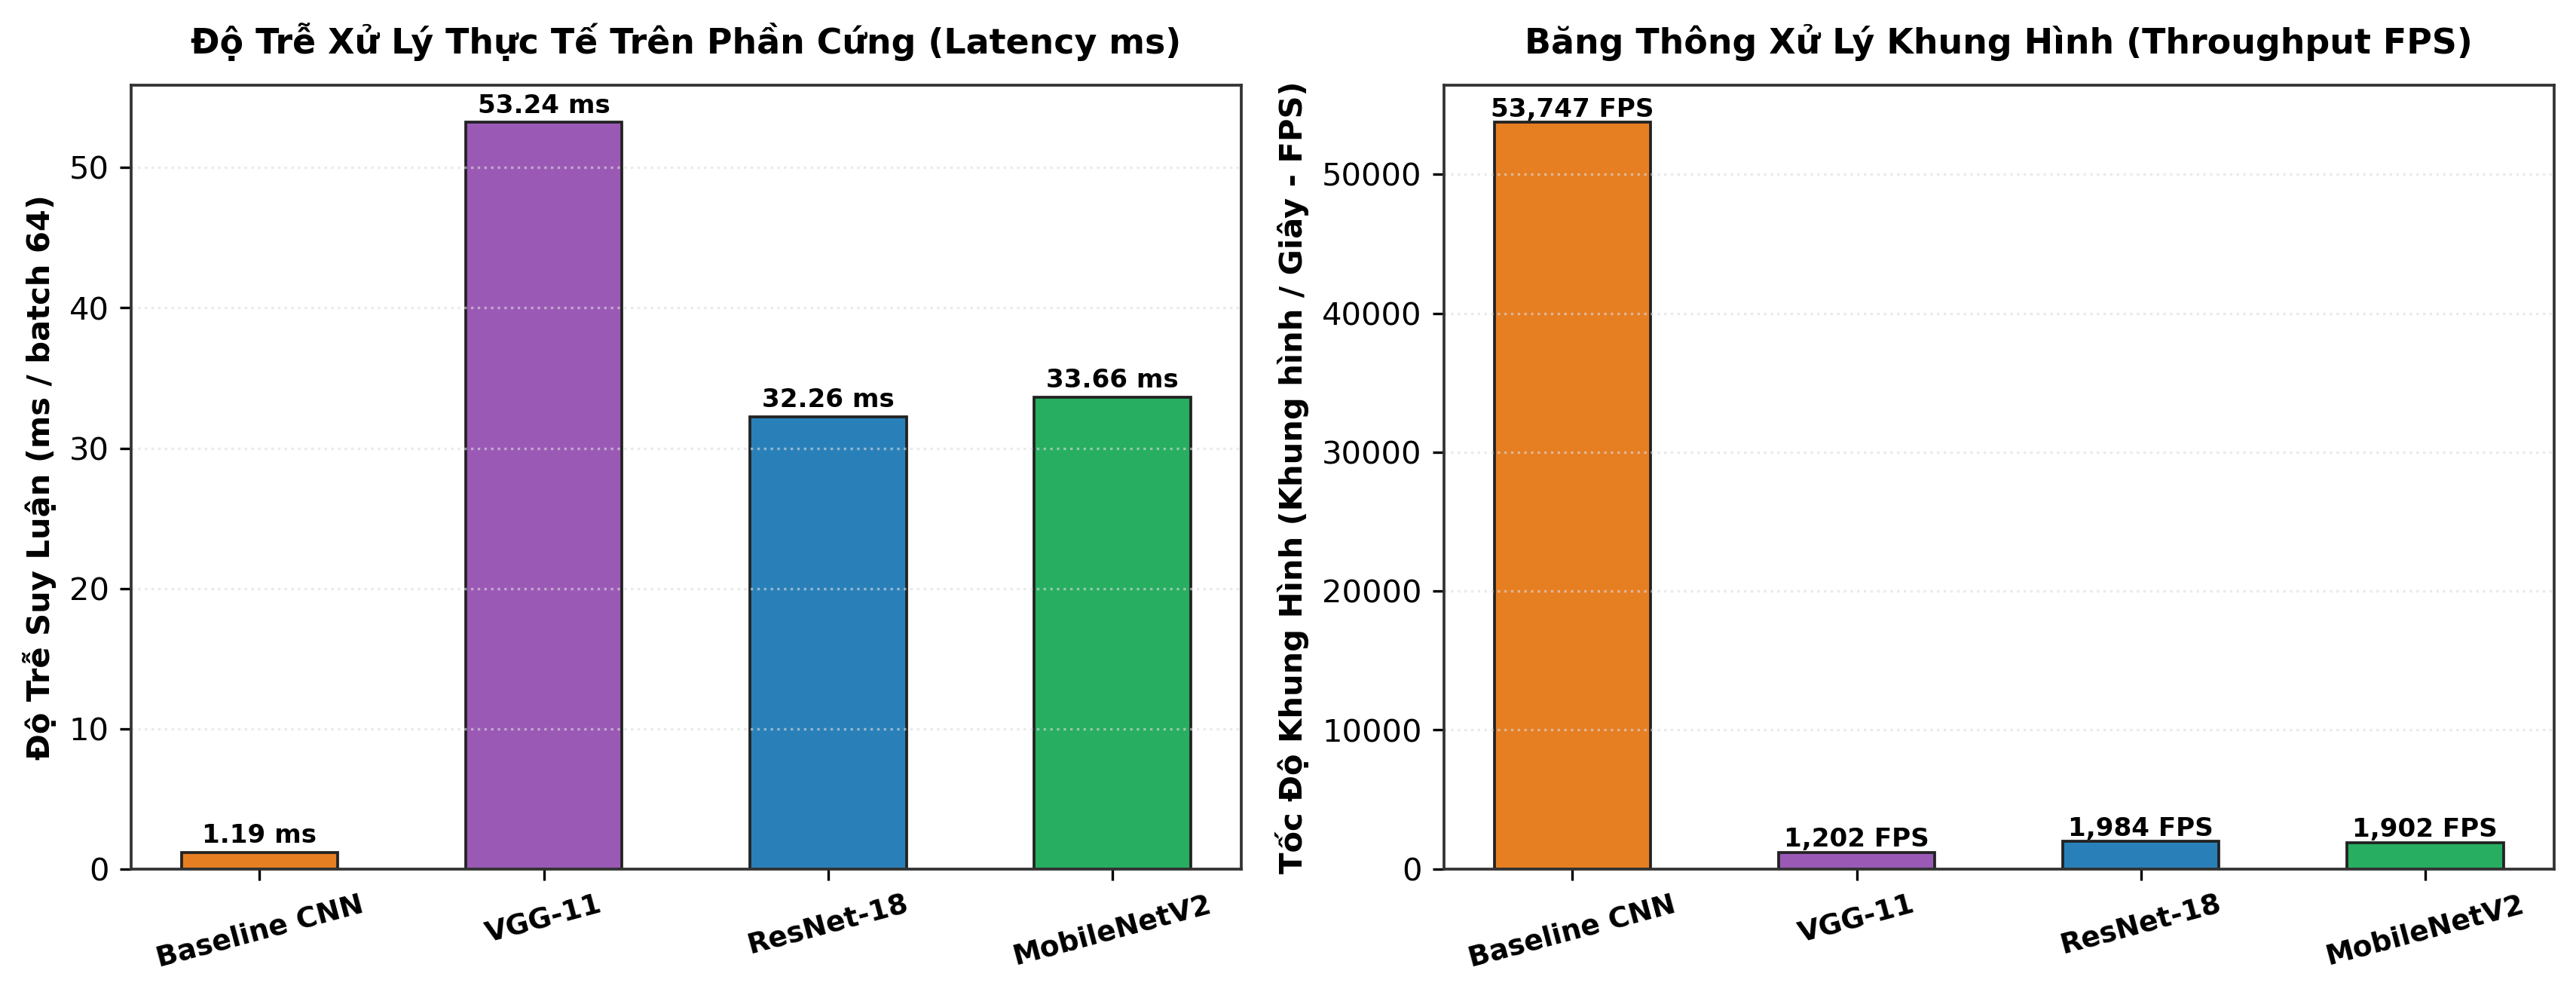
\includegraphics[width=0.90\textwidth]{images/fig508_latency_and_fps_benchmark.png}
    \caption{So sánh độ trễ xử lý (trái) và số khung hình mỗi giây FPS (phải).}
    \label{fig:latency_and_fps_benchmark}
\end{figure}

\begin{figure}[H]
    \centering
    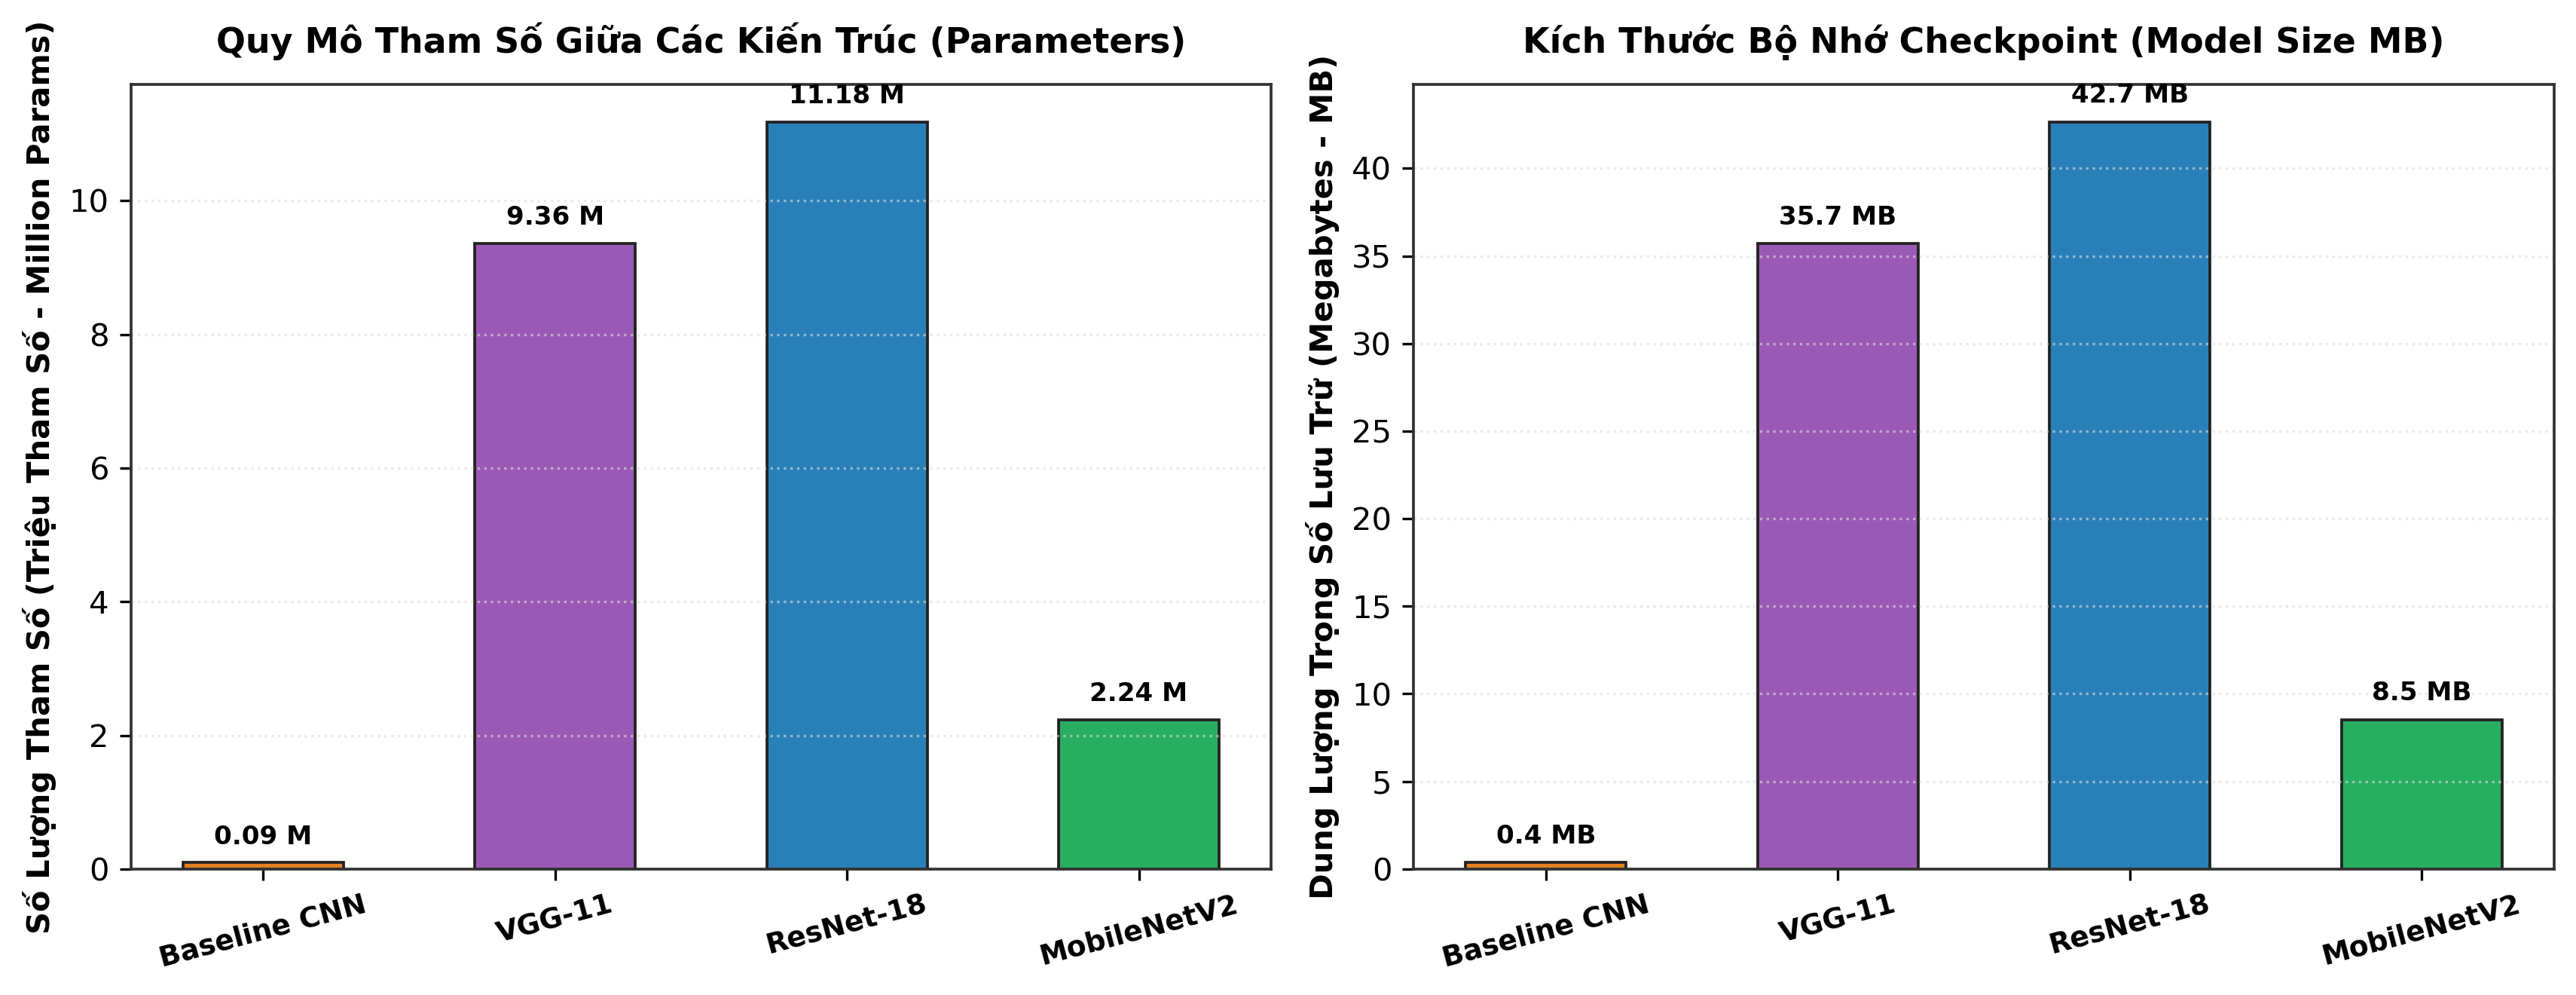
\includegraphics[width=0.90\textwidth]{images/fig509_model_parameters_and_checkpoint_size.png}
    \caption{So sánh số lượng tham số (trái) và dung lượng file checkpoint lưu trữ (phải).}
    \label{fig:model_parameters_and_checkpoint_size}
\end{figure}

\begin{figure}[H]
    \centering
    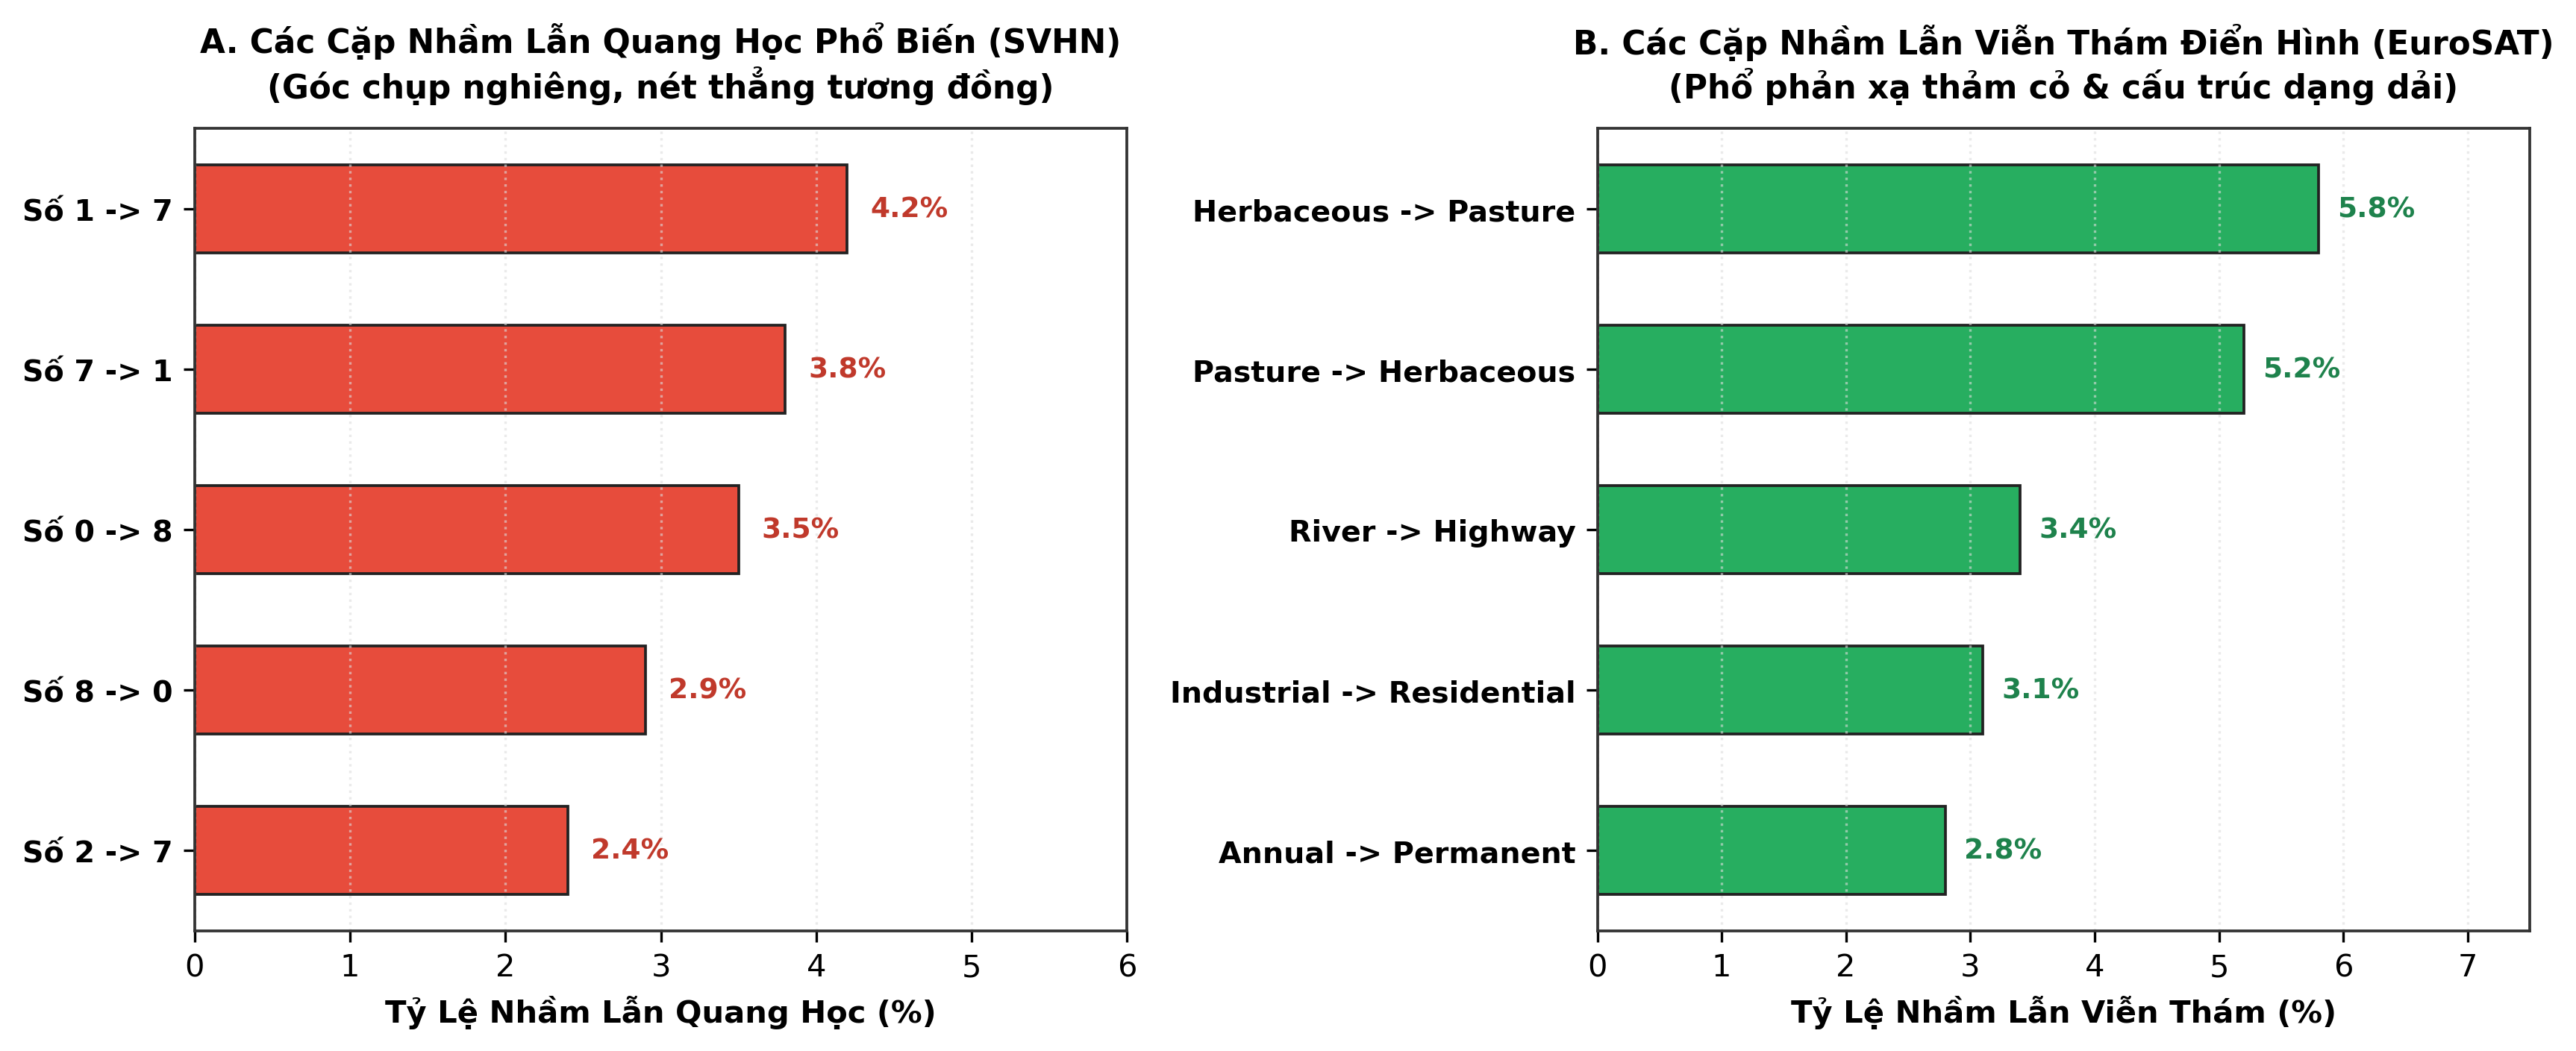
\includegraphics[width=0.90\textwidth]{images/fig510_confusion_matrix_error_analysis.png}
    \caption{Các cặp phân lớp dễ nhầm lẫn trên tập SVHN (trái) và EuroSAT (phải).}
    \label{fig:confusion_matrix_error_analysis}
\end{figure}

\subsection{Kết Luận Lựa Chọn Mô Hình Cho Từng Bài Toán}
\begin{enumerate}
    \item \textbf{Với dữ liệu dạng bảng (Diabetes):} Mạng 1D-CNN kết hợp hàm mất mát có trọng số là giải pháp phù hợp, đạt độ chính xác $95.52\%$, phát hiện được $77.00\%$ người bệnh và chạy cực nhanh ($152,000$ hồ sơ/giây).
    \item \textbf{Khi cần độ chính xác cao nhất trên ảnh:} ResNet-18 là lựa chọn hàng đầu, đứng đầu cả hai tập ảnh SVHN ($88.10\%$) và EuroSAT ($87.13\%$), huấn luyện ổn định nhờ đường tắt skip connection.
    \item \textbf{Khi triển khai trên thiết bị nhẹ hoặc cần tốc độ cực nhanh:} Baseline CNN hoặc MobileNetV2 là lựa chọn tối ưu nhờ kích thước nhỏ gọn (dưới $10\,\text{MB}$) và tốc độ xử lý hàng chục nghìn khung hình mỗi giây.
\end{enumerate}

% =========================================================================
% 5.6. TÓM TẮT CHƯƠNG 5
% =========================================================================
\section{Tóm Tắt Chương 5}
\label{sec:chapter5_summary}

Chương 5 đã hoàn thành việc huấn luyện và đánh giá thực nghiệm các mô hình nơ-ron tích chập trên 3 bộ dữ liệu:
\begin{itemize}[leftmargin=*]
    \item \textbf{Dữ liệu bảng Diabetes:} Mạng 1D-CNN kết hợp hàm mất mát có trọng số đạt $95.52\%$ accuracy, giải quyết tốt vấn đề mất cân bằng lớp.
    \item \textbf{Dữ liệu ảnh ngoại cảnh SVHN:} ResNet-18 đạt độ chính xác cao nhất $88.10\%$, VGG-11 bám sát với $87.62\%$.
    \item \textbf{Dữ liệu ảnh vệ tinh EuroSAT:} ResNet-18 dẫn đầu với $87.13\%$, Baseline CNN đạt kết quả tốt $81.23\%$ dù cấu trúc rất nhẹ.
    \item \textbf{Đối chuẩn tổng thể:} ResNet-18 cân bằng tốt nhất giữa độ chính xác và tài nguyên; Baseline CNN nhẹ và nhanh nhất; VGG-11 tốn nhiều tính toán nhất.
\end{itemize}


\end{document}
